 %%%%%%%%%%%%%%%%%%%%%%%%%%%%%%%%%%%%%%%%%% 
 % @File    : c:\Users\Administrator\Desktop\Econometrics\econometrics.tex
 % @Date    : 2020-08-28 19:53:28
 % @Author  : RankFan
 % @Email   : 1917703489@qq.com
 % -----
 % Last Modified: 2021-02-15 18:01:33
 % Modified By: Rank_fan
 % -----
 %%%%%%%%%%%%%%%%%%%%%%%%%%%%%%%%%%%%%%%%%% 

\documentclass[UTF8]{book}
 %%%%%%%%%%%%%%%%%%%%%%%%%%%%%%%%%%%%%%%%%% 
 % @File    : c:\Users\Administrator\Desktop\Econometrics\structure.tex
 % @Date    : 2021-02-11 15:14:30
 % @Author  : RankFan
 % @Email   : 1917703489@qq.com
 % -----
 % Last Modified: 2021-02-15 11:25:53
 % Modified By: Rank_fan
 % -----
 %%%%%%%%%%%%%%%%%%%%%%%%%%%%%%%%%%%%%%%%%% 

\usepackage{ctex}
\usepackage{type1cm}
\usepackage{ragged2e}

%====================================== 标题设置=============== ================================%
\usepackage{caption}  % 标题
\usepackage{subfig} % 子图
\usepackage{authblk} % 作者
\usepackage{tocbibind} % 目录
\usepackage[Glenn]{fncychap} % 章节封面设置

%====================================== 章节设置=============== ================================%
\usepackage{titlesec} % 可对标题的式样进行全面精细地设置。
\usepackage{indentfirst} % 设置缩进的距离
\usepackage[left=2cm,right=2cm,top=2.5cm,bottom=3cm]{geometry} % 页面边距

%====================================== 表格、图设置=============== ================================%

%\usepackage{color}
% \usepackage{tikz,pgfplots} % tikz绘制图
%\usepackage{mathpazo}

\usepackage{enumerate} % enumerate 环境
\usepackage{fancyref} % 交叉引用
\usepackage{graphicx} % 插入图片
\usepackage{algorithm} % 算法
\usepackage{bm} % 对公式字母进行加粗
\usepackage{listings} % 在LaTex中添加代码
\usepackage{mathrsfs} % 插入花体公式
\usepackage{array} % 矩阵
\usepackage{multirow,booktabs} % 表格多行
\usepackage{arraycols} % 设置array的列间距
\usepackage{threeparttable}
\usepackage{longtable}

%====================================== 数学公式设置=============== ================================%
% \usepackage{tocvsec2} % 标题目录由固定层次深度改为可变层次深度
% \usepackage[utf8]{inputenc} % 用来嵌入字体
% \usepackage{calc}

\usepackage{amsmath,amssymb} % 数学公式
\usepackage{datetime} % 时间
\usepackage{pdfpages} % 就是将PDF文件加入到封面位置
% \usepackage[colorlinks,citecolor=blue,linkcolor=blue,urlcolor=red,bookmarks, bookmarksnumbered]{hyperref} % hyperref 参数 breaklinks,
\usepackage{cases,empheq} % 大括号公式,有色公式 http://blog.sina.com.cn/s/blog_5e16f1770100h5gs.html
\usepackage{hyperref}
\hypersetup{ colorlinks,citecolor=blue,linkcolor=blue,urlcolor=red,
			bookmarks, bookmarksnumbered,
			unicode = true }


%=====================================================================================%
\setlength{\parindent}{2em} %===================首行缩进2字符

%================================== tikz ================================%
% \usetikzlibrary{arrows,shapes,intersections,angles,calc,quotes,through,decorations.text}
% \usetikzlibrary{shapes.geometric, arrows}

%================================== 标题设置 ================================%
\titlelabel{{\bf \S} ~ \thetitle \quad}

%================================== 自定义样式设置 ================================%
\lstdefinestyle{mystyle}{
	basicstyle=%
	\ttfamily
	\lst@ifdisplaystyle\small\fi
}

%================================== 设置中文字体 ================================%
\xeCJKsetup{AutoFakeBold=true}
\setCJKmainfont{FZShuSong-Z01}[BoldFont={FZHei-B01},ItalicFont={FZKai-Z03}]
\setCJKsansfont{FZHei-B01}
\setCJKmonofont{FZShuSong-Z01}
% \setsansfont{Verdana}

%================================== 设置英文字体 ================================%TeX Gyre Pagella
\setmainfont[Mapping=tex-text]{Times New Roman}%--------------------------------英文衬线字体
% \tikzset{elegant/.style={smooth,thick,samples=50,cyan}}
% \tikzset{eaxis/.style={->,>=stealth}}
% \definecolor[named]{color01}{rgb}{.2,.4,.6} % Color used in the title page

%================================== 盒子 ================================%TeX Gyre Pagella
% \newlength{\lablen}
% \setlength{\lablen}{0pt}
% \settowidth{\lablen}{2021 年 2 月 8 日}

%================================== newcommand ================================%
\newcommand{\topcaption}{%
		\setlength{abovecaptionskip}{0pt} % 标题前
		\setlength{belowcaptionskip}{2em} % 标题后
		\caption}
\newcommand*{\hei}{\CJKfamily{heiti}} 
\newcommand*{\num}{pi}
\newcommand{\thickhline}{%
	\noalign {\ifnum 0=`}\fi \hrule height 1pt
	\futurelet \reserved@a \@xhline}
\newcolumntype{"}{@{\hskip\tabcolsep\vrule width 1pt\hskip\tabcolsep}}
\newcommand*{\email}[1]{%
\normalsize\href{mailto:#1}{#1}\par
}

%===================================renewcommand ==============================================%
\renewcommand {\thetable} {\thechapter{}.\arabic{table}}
\renewcommand {\thefigure} {\thesection{}.\arabic{figure}}
\renewcommand\chaptermark[1]{\markboth{Chapter \thechapter\quad #1}{}}
\renewcommand\sectionmark[1]{\markright{\thesection\quad #1}}
\renewcommand{\today}{\number\year 年 \number\month 月 \number\day 日}
\renewcommand*{\Affilfont}{ \it }
\renewcommand\Authands{ and  } 
\setcounter{secnumdepth}{3}

%===================================设置中文章节标题==========================================================%
\renewcommand\sectionmark[1]{%
 \markright{\CTEXifname{\CTEXthesection——}{}#1}}

%===================================newtheorem ==========================================================%
\newtheorem{theorem}{$ \bf{{Theorem}}  $}[section]
\newtheorem{mydef}{Definition}[chapter]
\newtheorem{myproof}{Proof}[chapter]
\newtheorem{myexample}{Example}[chapter]
\newtheorem{mypty}{Property}[chapter]
\newtheorem{mycor}{Corollary}[chapter]

% =================================设置节标题==========================================================%
\numberwithin{equation}{section}

% ================================表格caption设置==========================================================%
\captionsetup[table]{%
	labelsep = quad ,  % title与font之间的距离
	name = 表 %表的名字
}
% ====================================================%

% \title{ \heiti 计量经济学知识总结 }
% \author[a]{RankFan  \thanks{fanxiaolong98@gmail.com} }
% \author[a]{MonicaRong \thanks{xmu2020wyr@gmail.com} }
% \affil[a]{ 公众号:经济知识综合}
% \date{\today}

\begin{document}

		\begin{titlepage}
			\centering % Center everything on the title page
			\scshape % Use small caps for all text on the title page
			\vspace*{1.5\baselineskip} % White space at the top of the page
		% ===================
		%	Title Section 	
		% ===================

			\rule{15cm}{1.6pt}\vspace*{-\baselineskip}\vspace*{2pt} % Thick horizontal rule
			\rule{15cm}{0.4pt} % Thin horizontal rule
			
				\vspace{0.75\baselineskip} % Whitespace above the title
		% ========== Title ===============	
			{	\Huge 计~量~经~济~学 ( Econometrics )\\ 
					\vspace{4mm}
				知~识~总~结 \\	}
		% ======================================
				\vspace{0.75\baselineskip} % Whitespace below the title
			\rule{15cm}{0.4pt}\vspace*{-\baselineskip}\vspace{3.2pt} % Thin horizontal rule
			\rule{15cm}{1.6pt} % Thick horizontal rule
			
				\vspace{1.75\baselineskip} % Whitespace after the title block
		% =================
		%	Information	
		% =================
			{\large Produced by: \href{https://person.zju.edu.cn/0087038}{蒋岳祥} \\
				\vspace*{1.2\baselineskip}
				jiangyuexiang@zju.edu.cn} \\
			    \vspace*{\baselineskip}
			{\large Editor: \href{https://blog.csdn.net/Rank_fxl?spm=1001.2101.3001.5343}{RankFan}\quad  MonicaRong \\
				\vspace*{\baselineskip}
				fanxiaolong98@gmail.com \quad 
				xmu2020wyr@gmail.com\\
				\vspace*{\baselineskip} 
				公众号:~ 经济知识综合\\
				\vspace*{\baselineskip}
			    { \it  \scshape Version~1.0} \\
				\vspace*{\baselineskip}
				\today} 
			\vfill
		If you come across any problems, Read other books for possible\\ \vspace{1mm}
		solutions or contact me at \url{fanxiaolong98@gmail.com} ~ \& ~ \url{xmu2020wyr@gmail.com} \\ \vspace{1mm}
		Happy Read-ing!
		\end{titlepage}
		%%%%%%%%%%%%%%%%%%%%%%%%%%%%%%%%%%%%%%%%%%%%%%%%%%%%%%%%%%%
		% \texorpdfstring{TEXstring}{PDFstring}
	\begin{sloppypar}
		% \maketitle
		\frontmatter
		 %%%%%%%%%%%%%%%%%%%%%%%%%%%%%%%%%%%%%%%%%% 
 % @File    : c:\Users\Administrator\Desktop\Econometrics\sections\NL.tex
 % @Date    : 2021-01-22 13:51:14
 % @Author  : RankFan
 % @Email   : 1917703489@qq.com
 % -----
 % Last Modified: 2021-02-15 14:21:38
 % Modified By: Rank_fan
 % -----
 %%%%%%%%%%%%%%%%%%%%%%%%%%%%%%%%%%%%%%%%%% 

 \chapter{Preface}

各位读者好,我现在是一名经管学科的在读研究生,在大三时看过浙江大学蒋岳祥老师的中级计量经济学,后来又看了部分高级计量经济学。
推荐资料:\href{https://bbs.pinggu.org/a-503441.html}{Econometrics Analysis} ;推荐课程:
蒋岳祥老师的\href{https://www.bilibili.com/video/BV1es411W7KU?from=search&seid=3253765381861883959}{中高级计量经济学},
厦门大学洪永淼老师的
\href{https://www.icourse163.org/course/XMU-1002606048}{高级计量经济学}  和
\href{https://www.bilibili.com/video/BV11t411A7bp}{概率论与统计学}

\vspace{0.5em}
我被蒋岳祥老师对于计量经济学所吸引了,蒋岳祥老师课程曾将“小概率”事件与佛学的“因果循环”联系在一起,顿时让我感受到计量经济学的“哲学”性质。

\vspace{0.5em}
后来我在网上搜集到蒋岳祥老师的讲稿,由于计量经济学课程公式很多,\LaTeX 在这方面又有很大的优势,历时半年多,我终于将蒋岳祥老师讲稿的主要内容整理
成这个总结。

\vspace{0.5em}
这个总结主要分为四个部分,第一部分:“基础” ;第二部分:“线性”;第三部分:“应用” ;第四部分:“附录”。

\vspace{0.5em}
非常感谢我的同学给予的支持,由于我的能力有限,在整理蒋岳祥老师讲稿时未免不出现一些错误,请各位读者见谅。


~ \ \
\\[3em]

\begin{flushright}
    RankFan \quad  \\ 
    \today
\end{flushright}


% \hfill {2021年2月8日}
		% \setcounter{page}{1}
		% \renewcommand{\thepage}{\Roman{page}}
		\thispagestyle{plain}
		\tableofcontents
		\newpage 
		\setlength{\baselineskip}{22pt}
		% \setcounter{page}{1}
		% \renewcommand{\thepage}{\arabic{page}}
		\pagestyle{headings}
		\mainmatter
		\part{基础}
			\chapter*{课程简介}

\section*{课程简介}
\noindent \textbf{课程号:}

\noindent \textbf{课程名称(含英文主):}研究生《中级计量经济学》(Intermediate Econometrics)

\noindent \textbf{学分:2}

\noindent \textbf{周学时:4}

\noindent \textbf{预修课程:}经济学、高等数学、概率论和数理统计

\noindent \textbf{内容简介:}

首先介绍计量经济学中必须具备的数学知识如高等代数中矩阵、概率论与数理统计中点估计、有效估计、一致估计、区间估计、假设检验、大样本与极限理论等。而后介绍古典线性回归模型、多元线性回归模型、带有线性约束的多元线性回归模型及其假设检验、正态线性统计模型的最大似然估计、古典线性的大样本理论、非球形扰动与广义最小二乘、异方差性、非线性回归模型等。

\noindent \textbf{选用教材或参考书:}

\noindent \textbf{教材:}William H. Greene, \href{https://bbs.pinggu.org/a-503441.html}{Econometrics Analysis}, fourth edition。

\noindent \textbf{参考书:}

\noindent 1.William H. Greene,经济计量分析,Econometrics Analysis 的翻译, 中国社会科学出版社。

\noindent 2.课件。 
	
\section*{教学大纲}
\noindent \textbf{课程号:}

\noindent \textbf{课程名称(含英文主):}研究生《中级计量经济学》(Intermediate Econometrics)

\noindent \textbf{学分:2}

\noindent \textbf{周学时:4}

\noindent \textbf{预修课程:}经济学、高等数学、概率论和数理统计

\noindent \textbf{一、课程的教学目的和基本要求:}

本课程为已具备经济学,概率论和数理统计以及初级计量经济学的研究生开设的《中级计量经济学》。目的是为他们今后在经济和金融领域能够独立开展科学研究和调查提供坚实的统计与计量经济学的方法与技巧。本课程的重点是使学生充分掌握和理解以下三个方面的知识与技能:

\noindent 1.计量经济学的理论与原理;

\noindent 2.计量经济学中广泛使用的统计推断知识,方法与技巧;

\noindent 3.掌握各种模型需要的条件与模型的局限性和适用性。

\noindent \textbf{二、课程内容与学时分配:}

\noindent 第一章 \ 引言
$ \cdots\cdots\cdots\cdots\cdots\cdots\cdots\cdots\cdots\cdots\cdots\cdots\cdots\cdots\cdots
\cdots\cdots\cdots\cdots\cdots\cdots\cdots\cdots\cdots\cdots\cdots \text{1学时} $
\begin{itemize}
	\setlength{\itemsep}{-2pt} 
	\item 计量经济学概念
	\item 为什么学计量经济学
	\item 计量经济学模型 
\end{itemize}	

\noindent 第二章 \ 矩阵的基础知识	
$ \cdots\cdots\cdots\cdots\cdots\cdots\cdots\cdots\cdots\cdots\cdots\cdots\cdots\cdots\cdots
\cdots\cdots\cdots\cdots\cdots\cdots\cdots\cdots\cdots \text{4学时} $
\begin{itemize}
	\setlength{\itemsep}{-2pt}
	\item 矩阵的概念与运算
	\item 矩阵的特征根与特征向量
	\item 矩阵的二次型与二项式
	\item 矩阵的微分
\end{itemize}

\noindent 第三章 \ 概率论与数理统计
$ \cdots\cdots\cdots\cdots\cdots\cdots\cdots\cdots\cdots\cdots\cdots\cdots\cdots\cdots\cdots
\cdots\cdots\cdots\cdots\cdots\cdots\cdots\cdots \text{4学时} $
\begin{itemize}
	\setlength{\itemsep}{-2pt}
	\item 随机变量与概率
	\item 分布函数与中心极限定理 
	\item 二元态分布与多元正态分布
	\item 样本与样本的分布函数
	\item 统计量及其分布
	\item 点估计
	\item 有效估计
	\item 一致估计
	\item 区间估计
	\item 假设检验
\end{itemize}

\noindent 第四章 \ 古典线性回归模型
$ \cdots\cdots\cdots\cdots\cdots\cdots\cdots\cdots\cdots\cdots\cdots\cdots\cdots\cdots\cdots
\cdots\cdots\cdots\cdots\cdots\cdots\cdots\cdots\text{4学时} $
\begin{itemize}
	\setlength{\itemsep}{-2pt}
	\item 古典线性回归模型与其假设条件
	\item 最小二乘回归
	\item 方差分析
	\item 最小二乘统计量的有限样本性质
	\item 预测
\end{itemize}	

\noindent 第五章 \ 多元线性回归模型
$ \cdots\cdots\cdots\cdots\cdots\cdots\cdots\cdots\cdots\cdots\cdots\cdots\cdots\cdots\cdots
\cdots\cdots\cdots\cdots\cdots\cdots\cdots\cdots \text{4学时} $
\begin{itemize}
	\setlength{\itemsep}{-2pt}	
	\item 多元线性回归模型与其假设条件
	\item 最小二乘回归
	\item 方差分析
	\item 最小二乘统计量的有限样本性质
	\item 预测	
\end{itemize}	
	
\noindent 第六章 \ 带有线性约束的多元线性回归模型及其假设检验
$ \cdots\cdots\cdots\cdots\cdots\cdots\cdots\cdots\cdots\cdots\cdots\cdots\cdots
 \text{4学时} $
\begin{itemize}
	\setlength{\itemsep}{-2pt}	
	\item 带有线性约束的多元线性回归模型与其假设条件
	\item 线性约束的检验
	\item 参数带有约束的最小二乘回归
	\item Wald检验
	\item 实例	
\end{itemize}	

\noindent 第七章 \ 正态线性统计模型的最大似然估计
$ \cdots\cdots\cdots\cdots\cdots\cdots\cdots\cdots\cdots\cdots\cdots\cdots\cdots\cdots\cdots
\cdots\cdots\cdots \text{4学时} $
\begin{itemize}
	\setlength{\itemsep}{-2pt}	
	\item 模型及其假设条件
	\item 模型求解
	\item 与最小二乘估计量的比较	
\end{itemize}		
	
\noindent 第八章 \ 古典线性回归的大样本理论
$ \cdots\cdots\cdots\cdots\cdots\cdots\cdots\cdots\cdots\cdots\cdots\cdots\cdots\cdots\cdots
\cdots\cdots\cdots\cdots\cdots \text{4学时} $
\begin{itemize}
	\setlength{\itemsep}{-2pt}
	\item 最小二乘统计量的有限样本性质
	\item 古典回归模型的渐近分布理论
	\item 最小二乘估计量的渐近正态性
	\item 标准检验统计量的渐近行为
\end{itemize}	
	
\noindent 第九章 \ 非线性回归模型
$ \cdots\cdots\cdots\cdots\cdots\cdots\cdots\cdots\cdots\cdots\cdots\cdots\cdots\cdots\cdots
\cdots\cdots\cdots\cdots\cdots\cdots\cdots\cdots\cdots \text{2学时} $
\begin{itemize}
	\setlength{\itemsep}{-2pt}
	\item 非线性回归模型
	\item 可供选择的几个统计量
	\item 假设检验与参数约束
	\item Box-Cox 变换
\end{itemize}		
	
\noindent 第十章 \ 异方差性
$ \cdots\cdots\cdots\cdots\cdots\cdots\cdots\cdots\cdots\cdots\cdots\cdots\cdots\cdots\cdots
\cdots\cdots\cdots\cdots\cdots\cdots\cdots\cdots\cdots\cdots\cdots \text{2学时} $
\begin{itemize}
	\setlength{\itemsep}{-2pt}
	\item OLS估计的探讨
	\item 异方差性的检验
	\item GLS估计
	\item 二阶段估计
\end{itemize}			
			\chapter{导言}

学习计量经济学应该准备什么?怎么去做?首先推荐浙江大学
蒋岳祥老师的\href{https://www.bilibili.com/video/BV1es411W7KU?from=search&seid=3253765381861883959}{中高级计量经济学},厦门大学洪永淼老师的
\href{https://www.icourse163.org/course/XMU-1002606048}{高级计量经济学}  和
\href{https://www.bilibili.com/video/BV11t411A7bp}{概率论与统计学}。

\section{什么是计量经济学}

计量经济学是由挪威经济学家R.Fisher在三十年代首先创立的一门学科,是关于运用统计方法测量经济关系的艺术与科学,已经成为现代经济学的重要组成部分之一。

如果要给{\bf{计量经济学(Econometrics)}}下一个较为确切的定义,我们可以这样界定:

计量经济学是这样一门学科,它根据以往历史的经济资料与数据,从经济理论出发,运用数理统计的分析方法对经济关系建立经济计量模型,并依据所建立的模型对经济系统进行结构分析,经济预测和政策评价。所以计量经济学涉及数学学科中的统计学领域和经济学领域,统计学与经济理论是计量经济学的两块基石。

经济现象包罗万象,影响经济的因素有很多,如果我们企图将所有的因素作为研究的对象,我们可能什么结论也得不到,研究经济问题的一般方法是:我们总是选用最重要的因素变量而屏弃一些非本质的因素(变量),还需要了解哪些经济现象是有待解释的,哪些重要因素是有助于解释这些经济现象的,如何度量量化那些因素,并努力寻求它们之间存在的数量关系,并用统计推断来检验这些关系,
如\fref{fig:Econometrics}。

计量经济学的研究内容:随机现象,客观事物所反映的规律。

\begin{figure}[!htbp]
	\centering %居中
	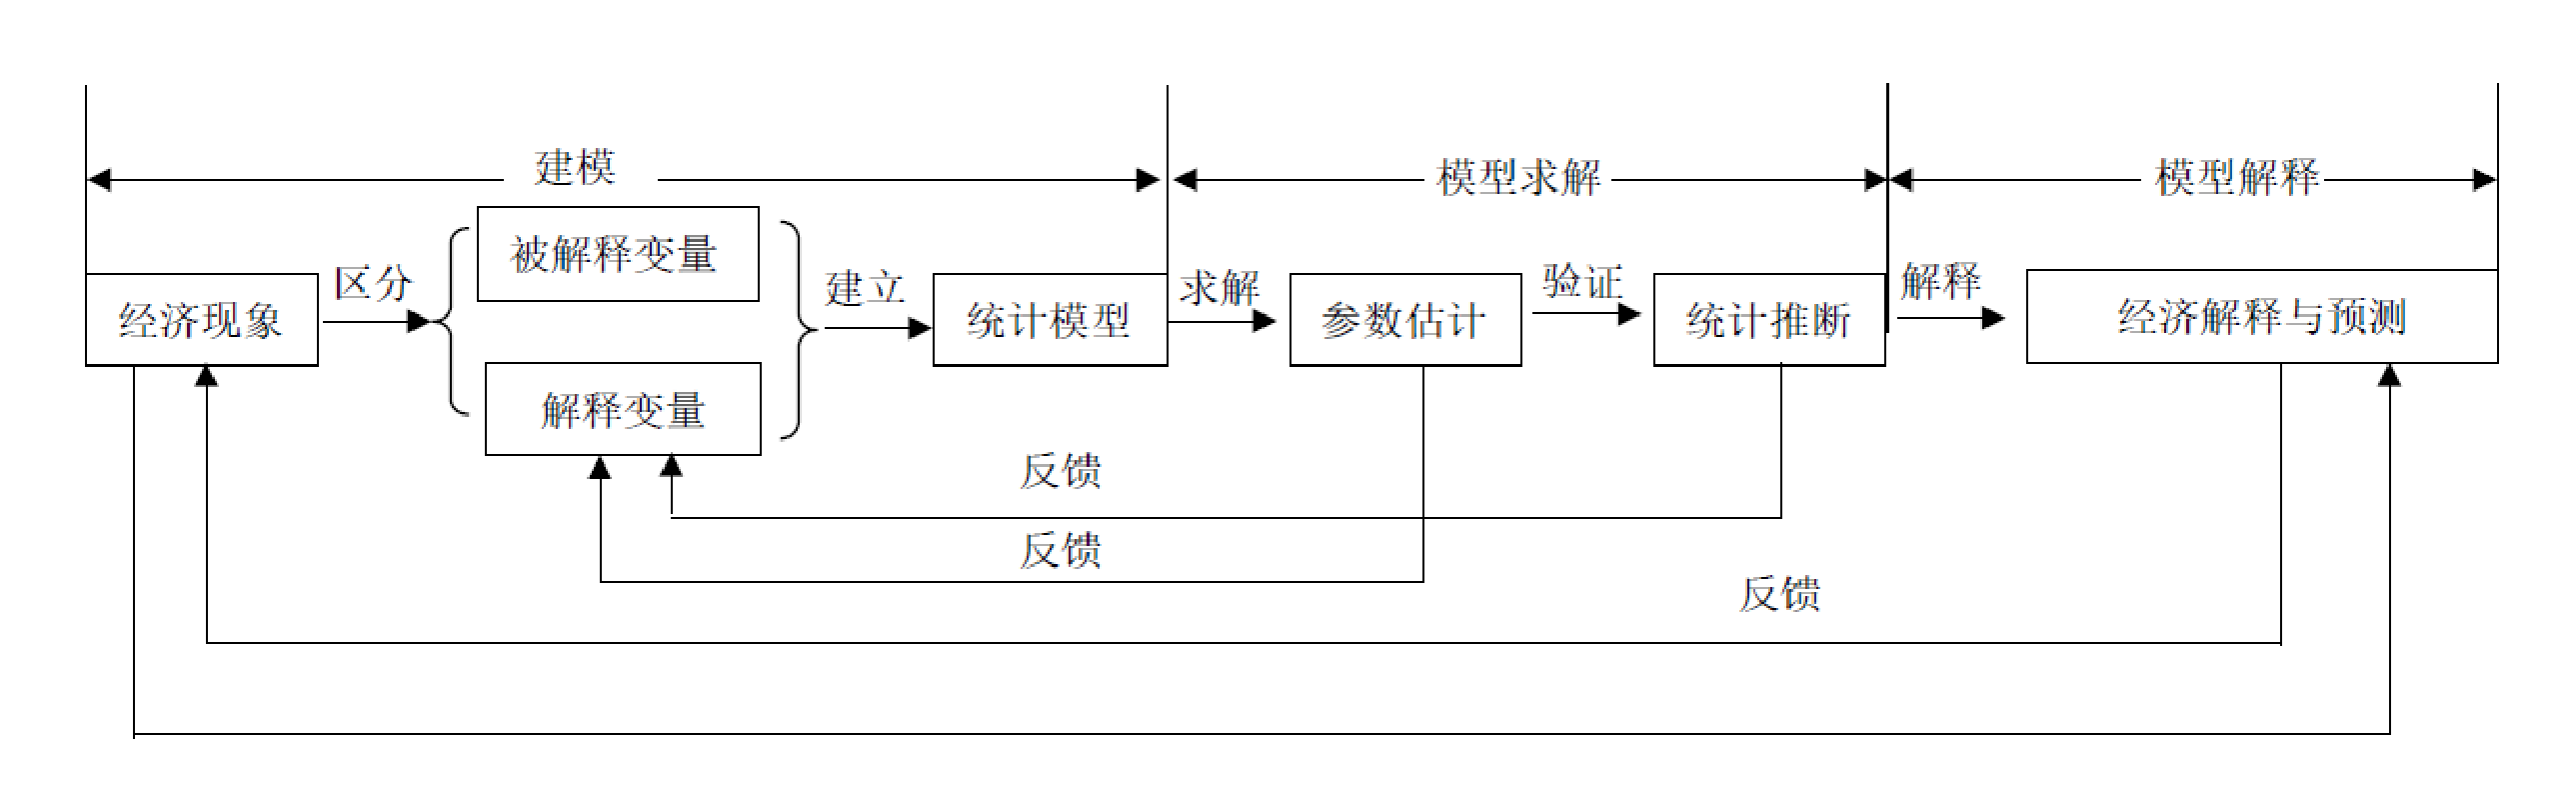
\includegraphics[width=0.9\textwidth]{Econometrics.eps}
	\caption{计量经济模型建立,求解,解释过程图}
	\label{fig:Econometrics}
\end{figure}

\section{随机现象的描述}
 工学和商学的思维模式与分析方法存在较大差异。一个是在确定下环境下少数可控变量关系的研究。另一个是研究在不确定性环境下无限且
不可控变量关系的问题。

实质上金融经济理论是研究不确定性的情况下,未来资源的如何最佳配置的问题。

银行为什么按揭贷款给年轻人?根据不同人来确定吗?未来的资产拿到今天来用。
研究随机现象是概率论与数理统计的知识。随机现象的处理,增加一个维度,例如基金经理投资成功的概率。
\begin{equation*}
	\lim_{n \to \infty} p^n =0  \qquad  \qquad  where \quad 0<p<1
\end{equation*}

研究对象的数据化,随机现象的描述——数据化。我们所看到的任何随机事件从理论上讲都可以通过将随机事件与数值联系。这样试验的结果就能有一个数来表示,
这个数是随着实验的结果的不同而变化,也即它是样本点一个函数,这种量被称为随机变量。

对于随机现象,最重要的是两件事,其一随机现象,其二出现结果的可能性。从而用来描述随机变量的大小变化和变化的可能性都可以量化。

随机现象 $A_1 , A_1 ,\cdots \cdots A_N $,为$ \boldsymbol{ A }$事件的集合体。$ I_{A_i} $ 表示事件是否发生。
	\begin{eqnarray}
		\boldsymbol{A} & =  & A_1  \cup  A_2 \cup A_3 \cup \cdots \cdots A_n  \notag\\ 
		& =  & \boldsymbol{A \Omega} = \boldsymbol{A}\sum_{i = 1}^{n} A_i = \sum_{i = 1}^{n} \boldsymbol{A} A_i \notag \\
		P(\boldsymbol{A}) & =  & P(\sum_{i = 1}^{n} \boldsymbol{A} A_i ) = 
		\sum_{i = 1}^{n} P(\boldsymbol{A} A_i) = \sum_{i = 1}^{n} P(\boldsymbol{A})P( A_i) \notag 
	\end{eqnarray}

\section{数据本质与统计规律}
概率论研究的分布函数,反映了事物变化和概率结合在一起。研究变量分为连续性变量,离散性变量。
计量经济学的三个定义,一是研究变量的分布函数,即古人所说的易,变化和概率(可能性)。
\begin{eqnarray}
	F(\mathrm {X} ) \quad & =  & P(\rm {X} \le \mathit{x} ) = \int_{-\infty }^{\mathit{x} } f(x)dx \notag \\
	F(\mathit{x_2}) - F(\mathit{x_1}) & =  &P(\mathit{x_1} <\rm X<\mathit{x_2}) \notag  \\
	\rm { Y }  & =  & X\beta + \varepsilon \qquad  \varepsilon \sim N(0,\sigma^ 2) 
\Longrightarrow Y ~\sim ~N(X\beta,\sigma^ 2)
\end{eqnarray}


计量模型估计$ \boldsymbol{\beta} , \ \ \varepsilon^2 \longrightarrow  $ 求Y的分布函数。
在均值附近变化一点,概率变化会很大。我国“古代思想”的概率论数据是基于随机现象的产生和发展得到的记录了事物发展的轨迹得到的数据,
不一定能够反映事物的本质不利用数据是否可以分析事物就是我们所说的玄学。

\subsection{数据的一般属性 } 

$  X_1,X_2,X_3,\cdots\cdots,X_n ~\sim ~F_{\theta} ~ (\mathit {x} ) $ 表明
$  X_1,X_2,X_3,\cdots\cdots,X_n  $ 独立同分布,

研究一个事物的要求分布函数,回归即是求分布函数,数据的分布($ \rm {X} \sim F_{\theta} (\mathit {x} $) )获得全样本是小概率事件,样本数据$ \Longrightarrow $ 母本数据。
\begin{eqnarray}
	\lim_{n \to \infty} \left \{ 
	\rm P \left (  X  =  \frac{1}{n} \sum X_i \le \mathit{x}  \right ) \right \}  
	 =  G_{\theta} \left( \mathit{x} \right) \sim \rm N(\mu,\sigma ^2) \notag 
\end{eqnarray}

$  n \to \infty $ 即为大样本,$ \rm \mu = \mathbb{E}(X) \sigma ^2 = var(X)$
平均属性$ \longrightarrow $ 平均的分布函数,查表时需进行标准化。哲学思想:天下乌鸦一般黑,事物随机现象的平均属性都服从正态分布。特例黑天鹅事件,
\begin{eqnarray}
	\rm P \left ( \frac{X-\mu}{\sigma }  \right )  \sim N (0,1) \notag
\end{eqnarray}

\subsection{数据的本质属性 } 

Fisher \&  Tippett 1928年已经完成,其极限分布只有三种类型。既所谓的极值分布是下列三种类型中的一种。最大值分布的特征事物的本质特征,事物最基本的本质。
\begin{eqnarray}
	\rm P \left [ max (X_1,X_2,X_3,\cdots \cdots X_n) \right ] < \it x \notag \\
	\lim_{n \to \infty} \rm P \left [ max (X_1,X_2,X_3,\cdots \cdots X_n) \right ] = ? \notag 
\end{eqnarray}
\begin{enumerate}
	\item \quad  Frechet分布 $ \Leftrightarrow   \rho > 0$
	\item \quad  Gumbel 分布 $ \Leftrightarrow   \rho < 0$
	\item \quad  Weibull分布 $ \Leftrightarrow   \rho = 0$
\end{enumerate}
\begin{equation*}
	 \rm min (X_1,X_2,X_3,\cdots \cdots X_n) = max (-X_1,-X_2,-X_3,\cdots \cdots -X_n)
\end{equation*} 

{\heiti{总结}}:假设研究对象是随机的,增加一个维度,用概率论的分布函数描述描述事物。

\begin{mydef}
研究对象的分布函数;
\end{mydef}
$$  \boldsymbol{\rm { Y }  = \beta^{\prime} X + \varepsilon } \qquad  \varepsilon \sim N(0,\sigma^ 2) 
      \Longrightarrow \boldsymbol{Y} \sim N(\boldsymbol{\beta^{\prime} X},\sigma^ 2) $$

\begin{mydef} 
	分部函数怎么确定?随机现象的平均属性基本相同,2008年金融危机后研究点,侧重于本质属性。MLE方法、OLS方法和矩估计等都可以估计参数 
	$ \boldsymbol{X} \sim F_{\theta} (\it \boldsymbol{x}) $
\[  \begin{cases}
		\rm P (\overline{X} < { \it x} )  \qquad \qquad \qquad  \ \ \qquad \Longrightarrow Law  \ \ of \ \ Large \ \ Numbers \\
		\rm P (max\left ( X_1,X_2\cdots \cdots X_n\right )  < { \it x} )   \Longrightarrow Law  \ \ of \ \ Large \ \ Numbers 
	\end{cases} \]

$ G_{X} (X) $ 可以用一个等式表示:
\[  H_{p}(\rm X) =  \begin{cases}
						\rm e^ {\left \{ -(1+\rho {\it x})^{-1/\rho} \right \} } \qquad   \qquad\Longrightarrow if  \ \ \rho \neq  0\\
						\rm e^ {\left \{ -e^{-x} \right \}}  \qquad \qquad  \qquad  \ \ \Longrightarrow if  \ \ \rho  =  0 
				    \end{cases} \]

$ \rho = 0 $ 状态就为太极(极限的极限),道的最高境界(无或双有)。数据是错的怎么办,利用古代人的做法,还原本质。
\begin{figure}[htb!]
	\centering
	\includegraphics[scale = 0.5 ]{Figs/Taiji.pdf}
	\caption{太极图}
\end{figure}

\end{mydef}

\section{数据的价值与《易经》}
回归包括线性回归和非线性回归,数据决定模型。计量经济学一般会求均值(一阶矩)和方差(二阶矩)。一般来说$ \overline{X}  \sim  N(\mu,\sigma^2) $。用样本去估计母体,t检验使用t统计量。为什么会使用t统计量。检验优先样本可以获得 $ \overline{x} \ \  , \ \   S^2 $

单个变量之间所表现出来的规律,但世界之间是有联系的,X对Y有无影响,$ \rm H_{0} : \boldsymbol{\beta} = 0 $ ,用t统计量。拒绝原假设时,$ \beta \neq 0 $。$ \beta = 0 $ 是不是小概率事件?
\begin{eqnarray}
	\boldsymbol{ Y  = \beta^{\prime} X + \varepsilon } \qquad  \varepsilon \sim N(0,\sigma^ 2) 
	\Longrightarrow \boldsymbol{Y} \sim N( \boldsymbol{\beta^{\prime} X},\sigma^ 2)   \notag \\ 
	\rm (X_1,Y_1) \quad  (X_2,Y_2) \quad  (X_3,Y_3)  \cdots \cdots (X_N,Y_N) 
	\Longrightarrow Regression \ \ Coefficient  \notag
\end{eqnarray}
	\begin{table}[htb!]
	\caption{两类错误}
	\centering
	\songti
	\begin{tabular}{c|c|c}
		\hline 检验状策 & $\mathrm{H}_{0}$ 为真 & $\mathrm{H}_{0}$ 非真 \\
		\hline 拒绝 $\mathrm{H}_{0}$ & 犯$ \rm\uppercase\expandafter{\romannumeral 1}$类错误 $(\mathrm{\alpha})$ & 正确 \\
		\hline 接受 $\mathrm{H}_{0}$ & 正确 & 犯 $ \rm\uppercase\expandafter{\romannumeral 2}$ 类错误 $(\beta)$ \\
		\hline
	\end{tabular}
    \end{table}

一个事情虽然说用很小,但未必不发生作用,发生时就会为黑天鹅事件,计量经济学的背景为不存在黑天鹅事件。
现实社会中一个政策把事物的性质可以发生改变。很多因素都存在着非回归的关系。

数据的两大属性:数据的一般属性和本质属性对应的反映事物的一般属性和本质属性,

任何真正反映事物发展轨迹的数据是和事物本质一样,有“性”,并同样存在同性恋的情况。
对于任何研究,首先要做定性分析,而非定量分析分析,任何事物都有“性”,“性”是事物的本质,而且可以做定量分析。
《易经》与统计学的关系,《易经》研究的是风险,规避统计学建立的模型分析和预测也是风险规避。
“易”是事物变化的统计规律,“易”是事物的变化和可能性。“易”变化的复杂和简单相统一,极限是科学的语言极限,是中心极限定理、小概率事件的基础。

\begin{myexample}
	传统文化为什么阻碍中国人的科学技术进步?中国偏向于小概率事件。
\end{myexample}
\begin{myexample}
	就业愿望的衡量。劳动参与率(Lobor Force Paticular Rate)。L为收益率,$ \varepsilon $ 为冲击。
	$$ LFPR = \alpha + \beta L + \varepsilon $$
\end{myexample}

可以有如下原假设: $ H_0 : \beta = 0 $ , $ H_0 : \beta < 0 $。将工资水平考虑到估计中,分析工资的挤出效应。
$$ LFPR = \alpha + \beta_1 L + \beta_2 FH + \varepsilon $$

{\heiti{计量经济学常用的表达式:}}
\begin{enumerate}[1)]
	\item $\varepsilon$ 假设
	\item $\hat{\alpha} \ \ \hat{\beta_1} \ \ \hat{\beta_2} $线性部分,$ \hat{\sigma^2} $随机部分
	\item $ H_0 : \beta_1 = 0 $ , $ H_0 : \beta_2 = 0 $
	\item $ H_0 : \beta_1 = \beta_2 =  0 $
	\item $ R^2 $ 拟合优度,判定系数
	\item 预测,随机现象。
\end{enumerate}

\subsection{回归的本质}

设随机变量$ \boldsymbol{\beta^{\prime} X, Y, X^{T}} =\left(X_{1}, \ldots, X_{m} \right) $是$ m $维随机向量,它是可以预先测量的,
希望通过$ \boldsymbol{X} $ 预测 $ \boldsymbol{Y} $, 也就是说要寻找一个函数$ \rm y= M \left(\it x_{1}, \ldots, \it x_{m}\right) $ 当X的观察值为x时,
就把$ \rm M(\it x) $作为对Y的预测值。当然一般总希望一个好的预测,其均方预测误差应达到最小。

均值处理随机性,$ \rm M(\it x) $与Y最大相关,此时相关系数最大。
\begin{eqnarray}
	\mathbb{E}[Y-L(X)]^{2} & = & \mathbb{E}[Y-M(X)]^{2} + \mathbb{E}[M(X)-L(X)]^{2}  \notag \\ 
	\rm \rho\left [ Y,M({\it x}) \right ] & = & \max_{L}\rho\left [ Y,L(X) \right ] \notag
\end{eqnarray}

设(X,Y)的分布密度函数是 $  f(x,y) $ , 设X的边际分布密度函数是 $  f_{1}(x) $ ,Y关于X的条件分布密度是:
\[ \rm Y = \begin{cases}
				f(x,y)/f_{1} (x)  \qquad \qquad f_{1} (x) \neq 0 \\
				0        \qquad  \quad  \qquad     \qquad \qquad f_{1} (x)= 0 
			\end{cases}  \]
%优化函数
	\begin{align*}
		& M(x) \underset{ \ \ = \ \ }{\Delta} E(Y / x)=\int y f(y / x) ~ d y\\
		&\mathbb{E}[Y-L(X)]^{2}=\iint \ldots \int[y-L(x)]^{2} f(x, y) ~ d x d y \\ 
		& 	= \iint \ldots \int[y-L(x)+M(x)-M(x)]^{2} f(x, y) ~ d x d y \\
		&	= \iint \ldots \int[y-M(x)]^{2} f(x, y) ~ d x d y\\
		&+2 \iint \ldots \int[y-M(x)][M(x)-L(x)] f(x, y) ~ d x d y\\
		&+\iint \ldots \int[M(x)-L(x)]^{2} f(x, y) ~ d x d y  \vspace{1em} \\
		\Longrightarrow \qquad
		& \iint \ldots \int[y-M(x)][M(x)-L(x)] f(x, y) ~ d x d y \\
		& =\iint \ldots \int[y-M(x)][M(x)-L(x)] f(y / x) f_{1}(x) ~ d y d x \\
		& =\int \ldots \int[M(x)-L(x)] f_{1}(x)\left[\int y f(y / x) ~  d y-M(x)\right] d x = 0
	\end{align*}
\begin{equation}
	\mathbb{E}[Y-L(X)]^{2} = \mathbb{E}[Y-M(X)]^{2} + \mathbb{E}[M(X)-L(X)]^{2}
\end{equation}

右边第一项与$ L(X) $无关,第二项大于等于零,它等于零的充要条件是$ M(X) = L(X) $, 
它表示当 $ M(X) = L(X) $时, $ \mathbb{E}[Y-L(X)]^{2} $达到最小值 $ \mathbb{E}[Y-M(X)]^{2} $。
在统计学上,我们称$ Y = M(X) = \mathbb{E}(Y|X)  $为Y关于X的回归曲线。
\begin{displaymath}
	min \ \  [Y - M(x)]^2 = \min_{L} \ \ [Y-L(x)]^2 
\end{displaymath}
% 定义定理写法
\begin{theorem}[条件均值]
	\begin{align*}
		M(x) & = \mathbb{E}(Y|X)	\\
		Y & = \mathbb{E}(Y|x) + [ Y-\mathbb{E}(Y|x) ] = \mathbb{E}(Y|x) + \varepsilon \ \ \ \ \mathbb{E}(\varepsilon) =  0 
	\end{align*}
\end{theorem}

 $ \mathbb{E}(\boldsymbol{\varepsilon}) \neq  0 $ 将会如何?当$ X,Y $满足二元正态分布时,可以得到一般线性回归,
 求 $ \boldsymbol{Y = \mathbb{E}(Y|x) + \varepsilon }$,即指导联合分布。
$$ \boldsymbol{Y} = F(\boldsymbol{\beta,X}) + \boldsymbol{\varepsilon} , \mathbb{E}(\boldsymbol{\varepsilon}) =  0,  
		\mathbb{E}(\boldsymbol{\varepsilon \varepsilon^{\prime}}) = \sigma^2 \boldsymbol{\Omega}  $$

  $ \mathbb{E} (\boldsymbol{\varepsilon \varepsilon^{\prime}} )$为协方差矩阵,
$ (\varepsilon_1,\varepsilon_2,\cdots,\varepsilon_n) $为样本点,OLS回归会假设服从正态性分布。随机变量之间的联系是通过协方差系数。
\begin{eqnarray}
	\rho_{XY}  & = & \frac{\mathbb{E}\Big((X-\mathbb{E}X)(Y-\mathbb{E}Y)\Big)}{\sqrt{DX}\sqrt{DY}} \notag \\
	\rm cov(\varepsilon_{i},X_{j} ) & = & 0 \notag \\ 
	\rm \rho_{Y,M({\it x})} ^2 & = &\frac{cov^2 \left [ \ \ {Y},E(Y|X) \ \  \right ] }{ var(Y)var\left [ \mathbb{E} (Y|X)\right ]} \notag \\ 
	& =  & \frac{cov^2 \left [ \ \ E(Y|X) ,E(Y|X) \ \  \right ] }{ var(Y)var\left [ E(Y|X)\right ]} \notag \\
	& =  & \frac{var\left [ E(Y|X)\right ] }{ var(Y)} = R^2 \notag \\
	\Longrightarrow \qquad \rm \widehat{R_{Y,\hat{Y}}^2} & =  &  \frac{SSR}{SST}  = \widehat{\rho_{Y,\hat{Y}}^2} 
\end{eqnarray}
 

统计学中求均值,方差,相关系数,$ \rho $为相关系数阵,是变量之间的关系网。
古典线性回归是对现实问题的简化再简化。样本数据一般会存在异方差问题,$ \sigma^2_1 \neq \sigma^2_2 $,如组间数据异方差。

自相关问题,一阶自回归模型。
\begin{displaymath}
	\boldsymbol{\Sigma} =\left(
	\begin{array}{ccccc}
	\sigma^{2} & \rho & \rho^{2} & \cdots & \rho^{n-1} \\ 
	\rho & \sigma^{2} & \rho & & \rho^{n-2} \\ 
	\rho^{2} & \rho & \sigma^{2} & & \vdots \\ 
	\vdots & & & \ddots & \rho \\ \rho^{n-1} & \cdots & & \rho & \sigma^{2}
	\end{array}  \right)
\end{displaymath}

ARCH(条件异方差),GARCH(广义条件异方差)。对 $ L(\alpha , \beta) $求偏导,得到
$ \widehat{\alpha}, \widehat{\beta} \Longrightarrow Y_{i} =  \widehat{\alpha} + \widehat{\beta} X_{i} + e_{i} $。
得到$ e_{1},e_{2},\ldots e_{n} $ 检验 $ \varepsilon  \sim  N(0,\sigma^2) $
$$  \boldsymbol{\Sigma} = \left(\begin{array}{cccc}
 \sigma_{1}^{2} & 0 & \cdots & 0 \\ 
 0 & \sigma_{2}^{2} & & \vdots \\ 
 \vdots & & \ddots & 0 \\ 0 & \cdots & 0 & \sigma_{n}^{2}
 \end{array} \right) $$
\begin{displaymath}
	Y_{i} = \alpha + \beta X_{i} + \varepsilon_{i}  \qquad
	L(\alpha , \beta) = \sum_{i=1}^n(Y_{i} -\alpha -\beta X_{i} )^2
\end{displaymath}
\begin{enumerate}
	\item$  X_{1},X_{2},\ldots  $\ \ $ \Longrightarrow Y $,利用联合分布$ f(X_{1},X_{2},\ldots X_{m})  \Longrightarrow L(\cdot) $
	\item $ Y = \beta X + \varepsilon \qquad H_0 : \beta_1 =0 / H_0 : \beta_2 =  0 $
	\item $ \varepsilon_1,\varepsilon_2,\ldots \varepsilon_n $,
			对于PRF,$ \mathbb{E}( \boldsymbol{\varepsilon} ) = 0  $
			$ \mathbb{E}( \boldsymbol{\varepsilon \varepsilon{\prime}} )  $= $ \sigma^2 \boldsymbol{\Omega} $是否满足。
	\item OLS。 $ L(\alpha , \beta) = \sum_{i=1}^n(Y_{i} -\alpha -\beta X_{i} )^2 \Longrightarrow Y 
	     =  \widehat{\alpha} + \widehat{\beta} X + e (Sample  \ \  Regression \ \ Function) $理解为条件回归+波动,一般有几个假定,就会有几个检验。
\end{enumerate}


\section{计量经济学实例}
\subsection{消费}

学过经济学中凯恩斯经济理论的人都知道,理论上说消费和收入存在着密切的联系,如果C表示消费,Y表示收入。则C与Y的关系,可用消费函数表示:
\begin{equation}
	C = f(Y)
\end{equation}

这样的函数满足:

1) \quad 边际消费倾向(MPC)位于0和1之间; 

2) \quad 平均消费倾向(APC)是随着收入的增加而减少。

\begin{eqnarray}
\frac{d \dfrac{C}{Y}}{d Y} & = & \frac{d\left(C \cdot \frac{1}{Y}\right)}{d Y} \notag \\ 
& = & \frac{d C}{d Y} \cdot \frac{1}{Y}-\frac{1}{Y^{2}} C \notag \\ 
& = & \frac{1}{Y}\left( \frac{d C}{d Y} -\frac{C}{Y}\right) \notag =\frac{1}{Y}\left( MPC -APC\right)<0
\end{eqnarray}

在现实经济社会中,消费与收入之间的关系很难确切地用方程(1)表示收入,我们所能采集到的数据往往受到这样那样的影响,我们可用随机扰动 来表示这些影响,所以,我们要对方程(1)要作适当调整,于是消费和收入之间的关系可以写成如下形式:
\begin{equation}
	C = f(Y,\varepsilon)
	\label{eq 1.5.2}
\end{equation}

其中$\varepsilon$是随机扰动。满足凯恩斯条件的 $\varepsilon$很多,无法枚举穷尽,但我们可以大致将它们分为线性模型与非线性模型两类。

\textbf{1. \quad 线性模型(Linear Model)}

方程\eqref{eq 1.5.2}的一个最简单的情况,是C与Y的线性关系,即:
\begin{equation}
	C = \alpha + \beta Y + \varepsilon
\end{equation}

如果我们现在从历史记录中或观察到N个样本,即($Y_t , C_t $ ),$ t=1,2,\cdots \cdots N $,于是我们有如下一组方程:
\begin{align*}
	&\mathrm{C}_{1}=\alpha+\beta \mathrm{Y}_{1}+\varepsilon_{1}\\
	&\mathrm{C}_{2}=\alpha+\beta \mathrm{Y}_{2}+\varepsilon_{2}\\
	&\cdots\cdots \\
	&\mathrm{C}_{\mathrm{N}}=\alpha+\beta \mathrm{Y}_{\mathrm{N}}+\varepsilon_{\mathrm{N}} 
\end{align*}

\textbf{2. \quad 非线性模型(Nonlinear Model)}

一般情况下,方程\eqref{eq 1.5.2}都是非线性的情况。现在我们假设0< $ \nu $ <1, MPC>0 ,即该模型满足凯恩斯的两个条件,这就是一个典型非线性模型。例如:
\begin{equation*}
	\mathrm{C}=\alpha+\beta \mathrm{Y}^{\nu}+\varepsilon
\end{equation*}
\subsection{奥肯定律}

奥肯定律:失业率每上升1\%,实际GDP下降2\%,这是线性回归的结果。

\subsection{Solow模型}
 带有$\mu$的Solow模型,西方经济理论在中国未必行得通,因为具体分布不同。希克斯提出中性技术条件。超越对数的生产函数,  \quad $\alpha$ 劳动的产出弹性,$\beta$资本的产出弹性。
	\begin{eqnarray}
		Y & = & A(t)f(L,K) =A_{0}e^{\mu t}f(L,K)  \nonumber \\
		\ln Y & = & lnA_{0} + \mu t + \ln f(L,K) 
	\end{eqnarray}
	\begin{eqnarray}
		\frac{d\ln Y} {dt} & = & \mu + \frac{d\ln f(L,K)}{dt}  \nonumber   \\
		\frac{d\ln Y} {Ydt}& = & \mu + \frac{\partial f}{f\partial L} \frac{dL}{dt} +\frac{\partial f}{f\partial K} \frac{dK}{dt} \nonumber \\ 
		& = & \mu +\frac{L}{f} \frac{\partial f}{\partial L} \frac{1}{L} \frac{dL}{dt} +
		\frac{L}{f} \frac{\partial f}{\partial K}\frac{1}{K} \frac{dK}{dt} \nonumber 
	\end{eqnarray}
	\begin{eqnarray}
		\frac{d \ln Y} {Ydt} & = & \mu + \frac{L}{A_{0}e^{\mu t}f} \frac{A_{0}e^{\mu t} \partial f}{\partial L} 
		\frac{1}{L} \frac{dL}{dt} +\frac{L}{A_{0}e^{\mu t}f} \frac{A_{0}e^{\mu t} \partial f}{\partial K}\frac{1}{K} \frac{dK}{dt} 
	\end{eqnarray}
	\begin{eqnarray}	
	\frac{\Delta Y} {Y}	& \stackrel{dt = 1}{=} &  \mu + \alpha \frac{\Delta L} {L} + \beta \frac{\Delta K} {K} \nonumber   \\
		1 &	=  &  \frac{\mu} {\Delta Y/Y} + \alpha \frac{\Delta L/L} {\Delta Y/Y} + \beta \frac{\Delta K/K} {\Delta Y/Y} \nonumber  
	\end{eqnarray} 
$$ \frac{\mu} {\Delta Y/Y}  \ \ is \ \ the \ \ Technological \ \ innovation $$ 

CD函数,$\alpha+ \beta = 1$ ,现对规模效应做检验,则$\beta = 1 - \alpha$
$$ 	\frac{\Delta Y} {Y}	=  \mu + \alpha \frac{\Delta L} {L} + (1 - \alpha) \frac{\Delta K} {K} \nonumber $$
			\chapter{数学基础}
\section{ 矩阵及其二次型(Matrix and its Quadratic Forms) }
\subsection{矩阵的基本概念与运算}
一个m×n矩阵可表示为:
\vspace{-1em}
$$  \boldsymbol{A}=\left[a_{i j}\right]=\left[\begin{array}{llll}
a_{11} & a_{12} &\cdots & a_{1 n} \\
a_{21} & a_{22} & \cdots &a_{2 n} \\
\cdots & \cdots & \cdots & \cdots \\
a_{m 1} & a_{m 2} & \cdots & a_{m n}
\end{array}\right] $$

矩阵的加法较为简单,若$ \boldsymbol{C} = \boldsymbol{A} + \boldsymbol{B} , c_{i,j} = a_{i,j} + b_{i,j}$。 但矩阵的乘法的定义比较特殊,若A是一个$ m×n_1 $的矩阵,B是一个$ n_1×n $的矩阵,则$ \boldsymbol{C}=\boldsymbol{AB} $是一个$ m×n $的矩阵,而且 ,一般来讲,$ \boldsymbol{AB} \neq \boldsymbol{BA} $,但如下运算是成立的:

 {a. \bf 结合律}(Associative Law)   $  \rm (\boldsymbol{AB}) \boldsymbol{C}=\boldsymbol{A}(\boldsymbol{BC}) $
 
 {b. \bf 分配律}(Distributive Law)  $  \rm \boldsymbol{A}(\boldsymbol{B+C})=\boldsymbol{AB}+\boldsymbol{AC} $
 
 向量(Vector)是一个有序的数组,既可以按行,也可以按列排列。 行向量(row vector)是只有一行的向量,列向量(column vector)只有一列的向量。如果α是一个标量,则$ \alpha \boldsymbol{A}=\left[\alpha a_{i j}\right]  $。
 
 矩阵$ \boldsymbol{A} $ 的转置矩阵(transpose matrix)记为$ \rm {\boldsymbol{A}}^{\prime}$ ,是通过把A的行向量变成相应的列向量而得到。显然
 $ (\rm {\boldsymbol{A}}^{\prime} )^{\prime}= \boldsymbol{A} $,而且$ \rm (\boldsymbol{A + B})^{\prime}= {\boldsymbol{A}}^{\prime} + {\boldsymbol{B}}^{\prime} $。
 
 乘积的转置( Transpose of  production ) \quad  $ \rm (\boldsymbol{AB})^{\prime}= {\boldsymbol{B}}^{\prime} {\boldsymbol{A}}^{\prime}   $ , 
        $ \rm (\boldsymbol{ABC})^{\prime}={\boldsymbol{C}}^{\prime}  {\boldsymbol{B}}^{\prime}  {\boldsymbol{A}}^{\prime}  $
 
 可逆矩阵(inverse matrix),如果n级方阵(square matrix)$ {\boldsymbol{A}} $和 ${\boldsymbol{B}}$,满足$ \boldsymbol{AB}=\boldsymbol{BA}=
 \boldsymbol{I} $。则称$ \boldsymbol{B} $、$ \boldsymbol{B}$ 是可逆矩阵,显然
 $ \rm \boldsymbol{A} = {\boldsymbol{B}}^{-1} $ ,  $ \rm \boldsymbol{B} = {\boldsymbol{A}}^{-1} $。如下结果是成立的:

  $$  \rm (\boldsymbol{A}^{-1}) ^{-1} = \boldsymbol{A},  \quad 
	   (\boldsymbol{A}^{\prime}) ^{-1} = (\boldsymbol{A}^{-1}) ^{\prime} , \quad 
	    (\boldsymbol{AB})^{-1} = \boldsymbol{B}^{-1} \boldsymbol{A}^{-1} $$
   
\subsection{特殊矩阵}

\begin{enumerate}[ 1) ] 
	\item 恒等矩阵(identity matrix):对角线上元素全为1,其余全为0,可记为$\boldsymbol{I}$;
	\item 标量矩阵(scalar matrix):即形如$ \alpha \boldsymbol{I} $的矩阵,其中$ \alpha $是标量;
	\item 幂等矩阵(idempotent matrix):如果矩阵 $ \boldsymbol{A} $ 具有性质 $ \boldsymbol{A} \cdot  \boldsymbol{A} = {\boldsymbol{A}}^{2} = \boldsymbol{A} $,
			这样的矩阵称为幂等矩阵。
	
	\begin{theorem}
		幂等矩阵的特征根要么是1,要么是零。
	\end{theorem}
	
	\item 正定矩阵 (positive definite)和负定矩阵(negative definite),非负定矩阵(nonnegative)或半正定矩阵(positive semi-definite),非正定矩阵(nonpositive  definite)或半负定矩阵(negative semi-definite);
	
		对于任意的非零向量 ,如有$ \vec{ \boldsymbol{x} }^{\prime} \boldsymbol{A} \vec{\boldsymbol{x}}>0 \quad(<0)$,则称A是正(负)定矩阵;
		如有 $  \vec { \boldsymbol{x}}^{\prime} \boldsymbol{A}  \vec {\boldsymbol{x}} \ge  0(\leq 0) $,非负(非正)定矩阵。
		如果A是非负定的,则记为$ \rm \boldsymbol{A} \ge 0 $;
		如果是正定的,则记为$ \rm \boldsymbol{A} > 0 $。
		协方差矩阵 是半正定矩阵,{\bf 几个结论: }
		
	\begin{enumerate}[ a) ]
		\item 恒等矩阵或单位矩阵是正定的;
		\item 如果 $ \boldsymbol{A} $ 是正定的,则$ \boldsymbol{A} ^{-1} $也是正定的;
		\item 如果 $ \boldsymbol{A} $ 是正定的,$ \boldsymbol{B} $ 是可逆矩阵,则 $ \boldsymbol{B}^{\prime} \boldsymbol{A} \boldsymbol{B} $ 是正定的;
		\item 如果 $ \boldsymbol{A} $ 是一个$ n \times m $矩阵,且$ n > m $,$ r(A) = m $ ,
				则 $ \boldsymbol{A}^{\prime} \boldsymbol{A}  $ 是正定的,$  \boldsymbol{A} \boldsymbol{A}^{\prime}  $ 是非负定矩阵。
	\end{enumerate}

	\item 对称矩阵(symmetric matrix):如果$ \boldsymbol{A} =  \boldsymbol{A}^{\prime} $ ,则$ \boldsymbol{A} $称为对称矩阵。
\end{enumerate}

\subsection{矩阵的迹(trace)}

一个n×n矩阵的迹被定义为它的对角线上的元素之和,记为$ tr(\boldsymbol{A}) $,则 $  tr(\boldsymbol{A}) = \sum_{i}^{n} a_{ii} $。
如下结论是显然的。

\begin{enumerate}[ 1) ]
	\item  $ {tr}(\alpha \boldsymbol{A}) = \alpha {tr}(\boldsymbol{A}) \cdots(\alpha \text { 是标量 }) \cdots  
	    Special \ \ case:  {tr}(\boldsymbol{I}) = n $  ;
	\item  $ {tr}\left( \boldsymbol{A} ^{\prime}\right) = {tr}(\boldsymbol{A}) $;
	\item  $ {tr}(\boldsymbol{ A + B }) = {tr}( \boldsymbol{A} )+{tr}( \boldsymbol{B} ) $;
	\item  $ {tr}(\boldsymbol{A B }) = {tr}(\boldsymbol{B A}), $ \qquad  
				特例  $ {tr}\left(\boldsymbol{A}^{\prime} \boldsymbol{A} \right) = \sum_{i = 1}^{n} \sum_{j = 1}^{n} a_{i j}^{2} $
	\item  循环排列原则: \quad $ tr(\boldsymbol{ABCD}) = tr(\boldsymbol{BCDA}) = tr(\boldsymbol{CDAB}) =tr(\boldsymbol{DABC}) $
	
	\begin{theorem}
		实对称矩阵$ \boldsymbol{A} $的迹等于它的特征根之和。
	\end{theorem}
	
	因为$ \boldsymbol{A} $是实对称矩阵,故有在矩阵$ \boldsymbol{C} $,使得 
	$  \rm \boldsymbol{C}^{\prime} \boldsymbol{A}  \boldsymbol{C}  = 
	\left(\begin{array}{ccc}
		\lambda_{1} 	&  		  		& \\
		&      			\ddots    		&\\
		&  				&     			\lambda_{n}
	\end{array} \right) $,
	其中 $ \boldsymbol{C}^{\prime}  \boldsymbol{C} = \boldsymbol{I} $ ,
	因此 $ \sum_{i=1}^{n} \lambda_{i}={tr}(\Lambda)
		={tr}\left(\boldsymbol{C}^{\prime} \boldsymbol{A} \boldsymbol{C}\right)
	    = {tr}\left(\boldsymbol{A} \boldsymbol{C}^{\prime} \boldsymbol{C}\right)={tr}(\boldsymbol{AI} )={tr}(\boldsymbol{A}) $
\end{enumerate}

	\subsection{矩阵的秩(rank)}

  一个矩阵A的行秩和列秩一定相等,一个矩阵的秩就可以定义为它的行秩或列秩,记为r(A),不加证明,我们给出如下结果:
  \begin{enumerate}[ 1) ]
 	\item $  r(\boldsymbol{A}) = r\left( \boldsymbol{A}^{\prime}\right) \leqslant \min( \rm row,col) $
	\item $  r(\boldsymbol{A})+r(\boldsymbol{A})-n_{1} \leqslant r(\boldsymbol{A B}) \leqslant \min (r(\boldsymbol{A}, r(\boldsymbol{A})) $ ,
	  其中$\boldsymbol{A}$、$\boldsymbol{B}$分别为$m \times n_1$、$n_{1} \times n$矩阵,
	  特例:如果$\boldsymbol{A}$、$\boldsymbol{B}$为 $n \times n$矩阵,而且$ \boldsymbol{AB=0}$,则 $ r(\boldsymbol{A})+r(\boldsymbol{A}) \le n $
 	\item $ r(\boldsymbol{A})=r\left(\boldsymbol{A} \boldsymbol{A}^{\prime}\right)=r\left(\boldsymbol{A}^{\prime} \boldsymbol{A}\right) $,其中 是$n \times n$的方阵
 	\item $ r(\boldsymbol{AB}) \le r(\boldsymbol{A})+r(\boldsymbol{B}) $
 	\item $ A $设 是$n \times n$矩阵,且$ \boldsymbol{A}^2 = \boldsymbol{I} $,则$ r(\boldsymbol{A+I})+r(\boldsymbol{A-I})=n $
 	\item $ A $设 是$n \times n$矩阵,且$ \boldsymbol{A}^2 = \boldsymbol{A} $,则$ r(\boldsymbol{A})+r(\boldsymbol{A-I})=n $
  \end{enumerate}

\subsection{统计量的矩阵表示}

向量可理解为特殊的矩阵。$ \vec{\boldsymbol{i}} $是一个其元素都为1的n维列向量,即$ \vec{\boldsymbol{i}} = (1,1,\cdots \cdots,1)$,
如果我们再假定$ \vec{\boldsymbol{x}} ^{\prime} = (X_1,X_2,\cdots \cdots,X_n) $,计量经济模型中的许多统计量就可以用矩阵的形式表示出来,很方便进行数学推导。

显而易见,$ \sum_{i=1}^{n} x_{i}=\vec{\boldsymbol{i}}^{\prime} \cdot \vec{\boldsymbol{x}}, \quad 
            \sum_{i=1}^{n} x_{i}^{2}=\vec{\boldsymbol{x}}^{\prime} \cdot \vec{\boldsymbol{x}} $,样本的均值与方差的矩阵表示如下:

  \begin{enumerate}[ 1) ]
	\item 样本均值矩阵表示:
	
	事实上 $ \vec{\boldsymbol{i}}^{\prime} \vec{\boldsymbol{i}} =n \text { 即 } 
				\dfrac{\vec{\boldsymbol{i}}^{\prime} \vec{\boldsymbol{i}}}{n}=1, \text { 而 } 
				\vec{\boldsymbol{i}} \vec{\boldsymbol{i}}^{\prime} =
	\left( \begin{array}{cccc}
	1 		& 1 			&\cdots	 		&	1 \\
	1 		& 1 			&\cdots	  		&	1 \\
	\cdots  & \vdots 		&\cdots 		&  \cdots \\
	1 	    & 1				&\cdots 		& 	1
	\end{array} \right),
	\overline{x} =\dfrac{\sum_{i=1}^{n} x_{i}}{n} =\dfrac{\vec{\boldsymbol{i}}^{\prime} \cdot \vec{\boldsymbol{x}} }{n}  $
	
	\item 样本方差矩阵表示:
	
	易知:  
	$ \left(\begin{array}{l}
		    \bar{x} \\ \vdots \\ \bar{x}
		   \end{array}  \right)
		=\vec{i} \bar{x}=\vec{i} \cdot \dfrac{\vec{i}^{\prime}  \cdot \vec{x} }{n}  
		=\dfrac{\vec{i} \vec{i}^{\prime} \vec{x}}{n}  $ 。  
	其中矩阵  $ \dfrac{1}{n} \vec{i} \vec{i}^{\prime} $ 是一个每个元素都为  $ \dfrac{1}{n} $的n阶
	阵, 从而  
	$ \left(\begin{array}
		{c}x_{1}-\bar{x} \\ 
		x_{2}-\bar{x} \\ 
		\vdots \\ 
		x_{n}-\bar{x}
	\end{array}\right)
	=(\vec{x}-\vec{i} \bar{x})=\left(\vec{x}-\dfrac{ \vec{i} \vec{i}^{\prime} \vec{x}}{n}\right)
	=\left(I-\dfrac{\vec{i} \cdot \vec{i}^{\prime}}{n} \right) \vec{x}  \triangleq  {\boldsymbol{M^{0}}} \vec{x} $
	
	矩阵$ \boldsymbol{M^{0}}  $的对角线上的元素为$ 1-\dfrac{1}{n} $,非对角线的元素为$ -\dfrac{1}{n} $,是一个对称矩阵。故样本方差:
	\begin{eqnarray}
			S^{2} & = &  \frac{1}{n} \sum_{i  =  1}^{n}\left(x_{i}-\bar{x}\right)^{2}  
			=  \frac{1}{n}(\vec{x}-\bar{x})^{\prime}(\vec{x}-\bar{x}) \notag \\
			& = &  \dfrac{1}{n} \vec{x} \cdot \boldsymbol{{M^{0}} ^{\prime }}  \boldsymbol{M^{0}} \vec{x}  
			=  \dfrac{1}{n} \vec{x} {\boldsymbol{M^{0}}^{2}} \vec{x}  =  \dfrac{1}{n} \vec{x}^{\prime}  \boldsymbol{M^{0}} \vec{x} \notag
	\end{eqnarray}	
	
	\begin{theorem}
		矩阵$  \boldsymbol{M^{0}} $是幂等矩阵。
	\end{theorem}
\end{enumerate}

\subsubsection {矩阵的二次型与多元正态分布}
   
	\begin{enumerate}[ 1) ]
		\item  \setlength{\parindent}{2\ccwd} 矩阵的二次型(Quadratic Forms)和线性变换(linear transferring)
		
		设$ \mathbb{P} $ 是一数域,一个系数在数域 $ \mathbb{P} $ 中的$ f \left(x_{1}, x_{2}, \cdots, x_{n} \right) $ 的二次齐次多项式
		\begin{eqnarray}
			f\left(x_{1}, x_{2}, \cdots, x_{n}\right)  =   
			a_{11} x_{1}^{2}+2 a_{12} x_{1} x_{2}+\cdots+2 a_{1 n} x_{1} x_{n}  \notag \\
			+a_{22} x_{2}^{2}+\cdots+2 a_{2 n} x_{2} x_{n}  \label{eq 2.1.1} \\
			\ldots \ldots \ldots \ldots . .  \notag \\
			+a_{n n} x_{n}^{2}  \notag 
		\end{eqnarray} 
		
		称为数域$ \mathbb{P} $ 上的一个n元二次型,或者,在不致引起混淆时简称二次型。例如
		$$ x_{1}^{2}+x_{1} x_{2}+3 x_{1} x_{3}+2 x_{2}^{2}+4 x_{2} x_{3}+3 x_{3}^{2} $$
		
		就是有理数域上的一个三元二次型,为了以后讨论上的方便,在\eqref{eq 2.1.1}中, $ x_{i} x_{j}(i<j) $的系数写在 $ 2a_{i} a_{j}$。而不简单地写成$ a_{i} a_{j}$。
		
		和在几何中一样,在处理许多其它问题时也常常希望通过变量的线性替换简化有关的二次型,为此,我们引入
		
		\begin{mydef} 
			设 $ x_{1}, \cdots, x_{n} ; \quad y_{1}, \cdots, y_{n} $是两组文字,系数在数域$ \mathbb{P} $ 中的一级关系式。
		\end{mydef}
		
		\vspace{-1em}
		\begin{eqnarray}
		\left\{\begin{array}{l}
		x_{1}  =  c_{11} y_{1}+c_{12} y_{2} +   \cdots + c_{1 n} y_{n}   \\
		x_{2}  =  c_{21} y_{1}+c_{22} y_{2} +   \cdots + c_{2 n} y_{n} \\
		\cdots  \cdots \\
		x_{n}  =  c_{n 1} y_{1}+c_{n 2} y_{2} + \cdots + c_{n n} y_{n}
		\end{array}\right.
		\label{eq 2.1.2}
		\end{eqnarray}
		
		称为由  $ x_{1}, \cdots, x_{n}, \quad x_{n} $ 到 $  y_{1}, \cdots, y_{n}  $
		的一个线性替换,或简称线性替换,如果系数行列式
		\vspace{-1em}
		$$ \left|c_{i j}\right| \neq 0 $$
		 % \vspace{-1.5em}
		那么线性替换 \eqref{eq 2.1.2}就称为非退化的。在讨论二次型时,矩阵是一个有力的工具,因此我们先把二次型与线性替换用矩阵来表示。
		
        令 $ a_{j} a_{i} = a_{i} a_{j} , \quad i <j$。由于 $ x_{j} x_{i} = x_{i} x_{j} $ 所以二次型
        \eqref{eq 2.1.2}
        	可以写成
        	 \begin{eqnarray}
	        		f\left(x_{1}, x_{2}, \cdots, x_{n}\right)  & =  & a_{11} x_{1}^{2}+a_{12} x_{1} x_{2}+\cdots+a_{1 n} x_{1} x_{n} \notag  \\
	        		&   & +a_{21} x_{2} x_{1}+a_{22} x_{2}^{2}+\cdots+a_{2 n} x_{2} x_{n} \notag \notag \\
	        		&   & \cdots \cdots \cdots \cdots \cdots \cdots\cdots \cdots \cdots \cdots \label{eq 2.1.3}  \\
	        		&   &  +a_{n 1} x_{n} x_{1}+a_{n 2} x_{n} x_{2}+\cdots+a_{n n} x_{n}^{2} \notag \\ 
	        		& = & \sum_{i  =  1}^{n} \sum_{j  =  1}^{n} a_{i j} x_{i}x_{j} \notag
			\end{eqnarray}
			
        把 \eqref{eq 2.1.3} 的系数排成一个n×n矩阵	
       \begin{eqnarray}
		\boldsymbol{A} & = & \left(
			\begin{array}{llll}
					a_{11} & a_{12} & \cdots & a_{1 n} \\
					a_{21} & a_{22} & \cdots & a_{2 n} \\
					\cdots & \cdots & \cdots & \cdots \\
					a_{n 1} & a_{n 2} & \cdots & a_{n n}
	       \end{array}\right)
	   \label{eq 2.1.4}
       \end{eqnarray}
       
       \eqref{eq 2.1.4} 就称为二次型\eqref{eq 2.1.3}的矩阵,因为$ a_{i j}  =  a_{j i}, \quad i, j  =  1, \cdots, n $。
       所以$ \boldsymbol{A} = \boldsymbol{A^{\prime}} $。我们把这样的矩阵称为对称矩阵,因此二次型的矩阵都是对称的。
       
       令 $  \boldsymbol{X} =\left(\begin{array}{c}
       x_{1} \\
       x_{2} \\
       \vdots \\
       x_{n}
       \end{array}\right)  $
       于是,二次型可以用矩阵的乘积表示出来,
       \vspace{-1em}
       \begin{eqnarray}
			\begin{array}{l}
				f\left(x_{1}, x_{2}, \cdots, x_{n}\right) = \boldsymbol{X^{\prime}} \boldsymbol{A} \boldsymbol{X} 
				\vspace{1em}  \\
					=  \left(x_{1}, x_{2}, \cdots, x_{n}\right)\left(
						\begin{array}{cccc}
							a_{11} & a_{12} & \cdots & a_{1 n} \\
							a_{21} & a_{22} & \cdots & a_{2 n} \\
							\cdots & \cdots & \cdots & \cdots \\
							a_{n 1} & a_{n 2} & \cdots & a_{n n}
						\end{array}\right)\left(
						\begin{array}{c}
							x_{1} \\
							x_{2} \\
							\vdots \\
							x_{n}
						\end{array}\right)
       \vspace{1em} \\
					=  \left(x_{1}, x_{2}, \cdots, x_{n}\right)\left(
						\begin{array}{l}
							a_{11} x_{1}+a_{12} x_{2}+\cdots+a_{1 n} x_{n} \\
							a_{21} x_{1}+a_{22} x_{2}+\cdots+x_{2 n} x_{n} \\
							a_{n 1} x_{1}+a_{n 2} x_{2}+\cdots+a_{n n} x_{n}
						\end{array}\right)\\
				=  \sum_{i=1}^{n} \sum_{j=1}^{n} a_{i j} x_{i} x_{j}  \notag
			\end{array}  
        \end{eqnarray}
        
        应该看到,二次型 \eqref{eq 2.1.1} 的矩阵$ \boldsymbol{A} $的元素 $ a_{i}a_{j} = a_{j}a_{i} $,
        正是它的$ x_{i}x_{j} = x_{j}x_{i} $项的系数的一半,因此二次型和它的矩阵是相互唯一决定的,由此还能得到,若二次型
        \begin{eqnarray}
			f\left( x_{1}, x_{2}, \cdots, x_{n}\right)  =  \boldsymbol{X^{\prime}} \boldsymbol{A} \boldsymbol{X}   
			   = \boldsymbol{X^{\prime}} \boldsymbol{B} \boldsymbol{X} \notag
		\end{eqnarray}
		
		且$ \boldsymbol{A} = \boldsymbol{A^{\prime}}, \boldsymbol{B} = \boldsymbol{B^{\prime}} $ 
		 则 $ \boldsymbol{A} = \boldsymbol{B} $。令:
        \begin{eqnarray}
			\boldsymbol{C} & = & \left(
				\begin{array}{llll}
					c_{11} & c_{12} & \cdots & c_{1 n} \\
					c_{21} & c_{22} & \cdots & c_{2 n} \\
					\cdots & \cdots & \cdots & \cdots \\
					c_{n 1} & c_{n 2} & \cdots & c_{n n}
				\end{array}\right), 
				\boldsymbol{Y}  =  \left(
				\begin{array}{l}
					y_{1} \\
					y_{2} \\
					\vdots \\
					y_{n}
				\end{array}\right)  \notag 
        \end{eqnarray}
        
        于是线性替换\eqref{eq 2.1.2} 可以写成
        
        \begin{eqnarray}
			\left(
				\begin{array}{l}
					x_{1} \\
					x_{2} \\
					\vdots \\
					x_{n}
				\end{array}\right) & = & \left(
				\begin{array}{llll}
					c_{11} & c_{12} & \cdots & c_{1 n} \\
					c_{21} & c_{22} & \cdots & c_{2 n} \\
					\cdots & \cdots & \cdots & \cdots \\
					c_{n 1} & c_{n 2} & \cdots & c_{n n}
				\end{array}\right)\left(
				\begin{array}{l}
					y_{1} \\
					y_{2} \\
					\vdots \\
					y_{n}
				\end{array}\right) \quad or \quad \rm \boldsymbol{X}=\boldsymbol{CY} \notag
        \end{eqnarray}
        
		\setlength{\parindent}{2\ccwd}  我们知道,经过一个非退化的线性替换,二次型还是变成二次型,现在就来看一下,替换后的二次型与原来的二次型之间有什么关系,
		也就是说,找出替换后的二次的矩阵与原二次型的矩阵之间的关系。
        \begin{eqnarray}
			Suppose \quad f\left(x_{1}, x_{2}, \cdots, x_{n}\right)  = \boldsymbol{X^{\prime}} \boldsymbol{A} \boldsymbol{X} , \quad \boldsymbol{A}   
			=  \boldsymbol{A^{\prime}}  \label{eq 2.1.5}
        \end{eqnarray}
        
        是一个二次型,作非退化线性替换
        \begin{eqnarray}
			\boldsymbol{X}   = \boldsymbol{CY}  \label{eq 2.1.6}
        \end{eqnarray}

        我们得到一个$ y_{1}, y_{2}, \cdots, y_{n}$ 的二次型
         $  \Longrightarrow \boldsymbol{Y^{\prime} B Y} $ 
         
        \setlength{\parindent}{2\ccwd} 现在来看矩阵B与A的关系。把\eqref{eq 2.1.6}代入\eqref{eq 2.1.5},有
        \begin{eqnarray}
			f\left(x_{1}, x_{2}, \cdots, x_{n}\right)  & = & \boldsymbol{ X^{\prime} A X } = 
			\boldsymbol{ (C Y)^{\prime} A(C Y) }  =  \boldsymbol{ Y^{\prime} C^{\prime} A C Y }  \notag \\
			& = &{ \boldsymbol{ Y^{\prime}\left(C^{\prime} A C\right) Y} } = \boldsymbol{ Y^{\prime} B Y } \notag
        \end{eqnarray}

        容易看出,矩阵$ C^{\prime} A C $也是对称的,事实上,
        \begin{eqnarray}
			\boldsymbol{ \left(C^{\prime} A C\right)^{\prime} } = \boldsymbol{ C^{\prime} A^{\prime} C^{\prime \prime} }
			= \boldsymbol{ C^{\prime} A C } \notag
        \end{eqnarray}

        由此,即得$ \boldsymbol{ B = C^{\prime} A C }$ 这就是前后两个二次型的矩阵的关系,与之相应,我们引入
        
        \begin{mydef}
			数域  $ \mathbb{ P } $ 上 $ n \times n $ 短阵  $ \boldsymbol{ A, B }$ 称为合同的,如果有数域  $ \mathbb{ P } $  上可逆的
        	$ n \times n $  矩阵  $ \boldsymbol{ C } $,使$ \boldsymbol{ B = C^{\prime} A C } $。
		\end{mydef}

        合同是矩阵之间的一个关系,不难看出,合同关系具有
        \begin{enumerate}[1)]
        	\item 反身性:$ \rm A = E^{\prime} A E $
        	\item 对称性:由$ \rm B = C^{\prime} A C $即得$ \rm B = (C^{-1})^{\prime} A C^{-1} $
        	\item 传递性:由$ \rm A_1 = C_{1}^{\prime} A C_{1} , A_2 = C_{2}^{\prime} A C_{2} $
        	即得$ \rm A_2 = (C_{1} C_{2})^{\prime} A (C_{1} C_{2}) $
        \end{enumerate}	
        \setlength{\parindent}{2\ccwd}	
        
        因之,经过非退化的线性替换,新二次型的矩阵与原二次型的矩阵是合同的。这样,我们就把二次型的变换通过矩阵表示出来,为以下的探讨提供了有力的工具。
        	
        最后指出,在变换二次型时,我们总是要求所作的线性替换是非退化的。从几何上看,这一点是自然的,因为坐标变换一定是非退化的,一般地,当线性替换。
        $$ \boldsymbol{ X = CY } $$

        是非退化时,由上面的关系即得
        $$ \boldsymbol{ Y = C^{-1}X } $$
        
        这也是一个线性替换,它把所得的二次型还原。这样就使我们从所得二次型的性质可以推知原来二次型的一些性质。
        \begin{theorem}
			定理:若$ \boldsymbol{ A } $是实对称矩阵,则存在可逆矩阵$ \boldsymbol{C} $,满足: 
			$ \begin{array}{l}
				\boldsymbol{ C^{\prime} A C}  = \boldsymbol{ \Lambda }=  \left(
					\begin{array}{ccc}
						\lambda_{1}               \\
						&            \ddots      &\\
						&              &      \lambda_{n}
					\end{array} \right)
			\end{array} $
		\end{theorem}
       \item 多元正态分布
       		\begin{enumerate}[a)]
       			\item 二元正态分布
       			\setlength{\parindent}{2\ccwd}
       			直观上,二元正态分布是两个正态随机变量的联合分布。如果两个随机变量$ X_1 $ 和$ X_2 $的联合密度函数为
					\begin{eqnarray}
					f\left(x_{1}, x_{2}\right) & =  &\frac{1}{2 \pi \sigma_{1} \sigma_{2} \sqrt{1-\rho^{2}}} 
					\exp \left\{-\frac{\Sigma }{2}\right\}^{-1} \notag \\
					where \quad -\infty<x_{1}, \quad x_{2}<\infty, &  &\quad \sigma_{1}>0, \quad \sigma_{2}>0, \quad-1<\rho<1 \notag \\
					\boldsymbol{\Sigma^{-1} } & = & \frac{1}{1-\rho^{2}} 
					\left[\left(\frac{x_{1}-\mu_{1}}{\sigma_{1}}\right)^{2}-2 \rho\left(\frac{x_{1}-\mu_{1}}{\sigma_{1}}\right)\left(\frac{x_{2}-\mu_{2}}{\sigma_{2}}\right)+\left(\frac{x_{2}-\mu_{2}}{\sigma_{2}}\right)^{2}\right] \notag
       			\end{eqnarray}
       			
				我们称$ X_1 $ 和$ X_2 $服从二元正态分布。通过计算可得$ X_1 $ 和$ X_2 $的边际分布分别为
				   $ \rm N(\mu_{1} ,\sigma_{1}^{2})$ , $ \rm N(\mu_{2} ,\sigma_{2}^{2})$。上式中的参数$ \rho $是$ X_1 $ 和$ X_2 $的相关系数。
       			
       			如果$ X_1 $ 和$ X_2 $服从二元正态分布,那么在给定$ X = \it x $ 的条件下$ X_2 $的条件分布也是正态的。它的条件密度函数为
       			\begin{eqnarray}
					f\left(x_{2} \mid x_{1}\right) \sim N\left(b, \sigma_{2}^{2}\left(1-\rho^{2}\right)\right) ,\quad 
					where \ \ b=\mu_{2}+\rho \frac{\sigma_{2}}{\sigma_{1}} \left(x_{1}-\mu_{1}\right) \notag
       			\end{eqnarray}
       			
       			条件均值$ \rm b =  \mathbb{E} \left(X_{2} \mid X_{1} \right) $是
				   $ \it x_{1} $的线性函数。并且,二元正态分布具有一个独特的性质,那就是如果$ \rho = 0 $,那么$ X_1 $ 和$ X_2 $是相互独立的。
				   这是由于当$ \rho = 0 $时,我们有 $ f\left(x_{2} \mid x_{1}\right) $。这对于一般的两个随机变量是不对的。
       			
       			有时如果把联合概率密度函数写成矩阵的形式,则从形式上来看就简单多了。记$ X^{\prime}=\left(X_{1}, X_{2}\right) $,那么二元正态概率密度函数可以写成如下的简单形式
       			\begin{eqnarray}
					f(x)  =  (2 \pi)^{-1}|\Sigma|^{-1 / 2} 
					 \exp \left\{-\frac{1}{2}(x-\mu)^{\prime} \Sigma^{-1}(x-\mu)\right\} \notag \\
       			where \ \ x=\left[
					   \begin{array}{l}
							x_{1} \\
							x_{2}
	       			   \end{array}\right], \mu=\left[
					   \begin{array}{l}
							\mu_{1} \\
							\mu_{2}
	       			   \end{array}\right], \boldsymbol{\Sigma}=\left[
					   \begin{array}{cc}
							\sigma_{1}^{2} & \sigma_{1} \sigma_{2} \rho \\
							\sigma_{1} \sigma_{2} \rho & \sigma_{2}^{2}
	       			   \end{array}\right] \notag
				   \end{eqnarray}
				   
       			\item 多元正态分布
       			
				   $ g(x)=\dfrac{1}{2 \pi^{\frac{n}{2}} \Sigma^{\frac{1 }{2}} }\exp \left\{-\frac{1}{2} { \boldsymbol{(x-\mu)^{\prime} \Sigma^{-1}(x-\mu)}} \right\}, 
				   \quad x \in \mathbb{R}^{n} $
       			这就是均值为$ \boldsymbol{ \mu }$ 协方差矩阵为$ \sum $的多元正态分布,记为$ \boldsymbol{ X } \sim  N(\boldsymbol{ \mu } , \boldsymbol{ \Sigma }) $
       			
       			\item 多元正态分布的二次型的分布
       			
       			如果$ \boldsymbol{X} \sim  N(\boldsymbol{\mu, \Sigma}) $,那么
       			$$ \boldsymbol{ Y=(X-\mu)^{\prime} \Sigma^{-1}(X-\mu) } \sim \chi_{(n)}^{2} $$
       			
				   这里n是$ \boldsymbol{X} $的维数。我们可以简单地证明这个结果。由于$ \boldsymbol{\Sigma} $是对称可逆矩阵,那么存在一个可逆的矩阵$ \boldsymbol{A} $,
				   使得 $ \boldsymbol{ A \sum A^{\prime}=I }$ 。我们有 $ \boldsymbol{ A X }\sim N(\boldsymbol{A \mu, I}), \boldsymbol{Z=A(X-\mu)} 
				   \sim N(0, \boldsymbol{I}) $ 
				   所以 $ \boldsymbol{ Y=Z^{\prime} Z=(X-\mu)^{\prime} \Sigma^{-1}(X-\mu)} \sim \chi_{(n)}^{2} $。
       		\end{enumerate}
	\end{enumerate}

   \subsection{幂等矩阵与二次型}
   幂等矩阵满足$ \boldsymbol{A^2=A} $的矩阵称为幂等矩阵。
   
   幂等矩阵可以是对称的,也可以是非对称的,但在我们计量统计学中,所研究的幂等矩阵都是对称的。与幂等矩阵的有关的结果有:
   \begin{enumerate}[1)]
   
   	\item 幂等矩阵的特征根要么是1,要么是零。
   	
 \begin{myproof}
		设 $ \lambda $ 是$ \boldsymbol{A} $的特征根,则  $ \boldsymbol{A E}=\lambda \boldsymbol{E}$ , 同时 
	$ \lambda \boldsymbol{E =A=A^{2}}=\lambda^{2} \boldsymbol{E} $ , \text { 故 } $ \lambda^{2}=\lambda$ , 
	从而 $  \lambda=1 $  或  $ \lambda=0$ 
 \end{myproof}
  
   	\item 唯一满秩的对称幂等矩阵是单位矩阵。
   	
  \begin{myproof}
	$ \because \boldsymbol{A^{2}=A} \Rightarrow \boldsymbol{A(I-A)}=0 \Rightarrow \boldsymbol{A^{-1} A(I-A)}=0 \Longrightarrow \boldsymbol{I=A} $
  \end{myproof}
   	\item $ \boldsymbol{A} $是幂等矩阵,则$\boldsymbol{I-A}$也是幂等矩阵,且秩$ \boldsymbol{(A)} $ + 秩$ \boldsymbol{(I - A)} $ = n。
   	\item 对称幂等矩阵的秩等于它的迹。
   	
   	\setlength{\parindent}{2\ccwd}
   	从而我们很容易知道$ \boldsymbol{M^{0}} $ 的秩。因$ \boldsymbol{M^{0}} $的每个对角元素都是 $ 1 - \dfrac{1}{n} $。因此
   	$ {tr} \left(\boldsymbol{M^{0}}\right) = n \cdot\left(1-\dfrac{1}{n}\right)
   	= n-1 = r\left(\boldsymbol{M^{0}}\right) $
   \item 
   $ \left.n S_{n}^{2} \text { 的服从 } \chi^{2}(n-1) \text { 分布(如果 } 
   \mathrm{X}_{i} \sim N(0, \boldsymbol{I}), i=1 ,\cdots , n\right) $ 
   
   这是因为:$ n S_{n}^{2}=\sum_{i=1}^{n}\left(x_{i}-\bar{x}\right)^{2}=\vec{x} \boldsymbol{M^{0}} \vec{x} \ \
   \text { 和 } \ \  r \left(\boldsymbol{ M^{0} }\right)=n-1 $
   
   \item $ \rm \boldsymbol{ M = I-X }\left( \boldsymbol{X^{\prime} X } \right)^{-1} \boldsymbol{ X^{\prime}} $ \quad $\boldsymbol{ X }$
   是一个$n \times m$的矩阵,秩
   $ \rm (\boldsymbol{X}) = m $,则 $\boldsymbol{M}$ 是幂等矩阵。
   \end{enumerate}

\subsection{微分及其矩阵的微分表示}
\begin{enumerate} [1、]
	\item 矩阵的微分
		\setlength{\parindent}{2\ccwd}
		如果$ y=f\left(x_{1}, x_{2}, \cdots, x_{n}\right) $ 或写成 $ y=f(x) $
		\begin{eqnarray}
		\begin{array}{c}
		\dfrac{\partial f(x)}{\partial x} = \left[\begin{array}{c}
		\partial y / \partial x_{1} \\
		\partial y / \partial x_{2} \\
		\vdots \\
		\partial y / \partial x_{n}
		\end{array}\right] = \left[\begin{array}{c}
		f_{1} \\
		f_{2} \\
		\vdots \\
		f_{n}
		\end{array}\right]
		\end{array} \notag
		\end{eqnarray}
		
		二阶偏导数矩阵为
		\begin{eqnarray}
		\frac{\partial f^{2}(x)}{\partial x \partial x^{\prime}}  =  \left[\begin{array}{cccc}
		\partial^{2} y / \partial x_{1} \partial x_{1} & \partial^{2} y / \partial x_{1} \partial x_{2} & \cdots & \partial^{2} y / \partial x_{1} \partial x_{n} \\
		\partial^{2} y / \partial x_{2} \partial x_{1} & \partial^{2} y / \partial x_{2} \partial x_{2} & \cdots & \partial^{2} y / \partial x_{2} \partial x_{n} \\
		\cdots & \cdots & & \cdots \\
		\partial^{2} y / \partial x_{n} \partial x_{1} & \partial^{2} y / \partial x_{n} \partial x_{2} & \cdots & \partial^{2} y / \partial x_{n} \partial x_{n}
		\end{array}\right] \notag
		\end{eqnarray}
		
		特别地,如果 $ y = \boldsymbol{ a^{\prime} x=x^{\prime} a }=\sum_{i=1}^{n} a_{i} x_{i} $,那么
		\begin{eqnarray}
		\frac{\partial \left( \boldsymbol{ a^{\prime} x } \right) }{ \partial \boldsymbol{x} }  =  
		\frac{\partial \left( \boldsymbol{ x^{\prime} a } \right) }{ \partial \boldsymbol{x} }  =  a \notag
		\end{eqnarray} 
		 
		同样地可得
		\begin{eqnarray}
		\frac{\partial \boldsymbol{A x}}{\partial \boldsymbol{x}}  =  \boldsymbol{A^{\prime}}  \notag
		\end{eqnarray}
		
		如果A是对称矩阵,那么
		\begin{eqnarray}
		\frac{\partial \boldsymbol{ x^{\prime} A x} }{\partial \boldsymbol{x}}  = 2 \boldsymbol{ A x } = \left( \boldsymbol{ A+A^{\prime} }\right) x \notag
		\end{eqnarray}
		
		{\bf 思考题:}
		
		1、证明:$ {tr}\left( \boldsymbol{ A A^{\prime} }\right) = \sum_{j = 1}^{n} \sum_{j=1}^{n} a_{i j}^{2} $
		
		2、证明矩阵$ \boldsymbol{M^{0}} $是幂等矩阵。
		
		3、如果$  L_{1} $、 $L_{2} \cdots L_{\mathrm{n}}  $ 的百分比变动较小$   \Delta L_{1}, \cdots \Delta L_{n} $
		
		如果 $  Y_{1}$ 、$ Y_{2} \cdots Y_{\mathrm{m}} $  巾百分比变动较小 $  \Delta Y_{1}, \cdots \Delta Y_{m} $
		则如下计算公式是否可行?
		
		\quad a) $  \Delta\left(L_{1}, L_{2} \cdots L_{n}\right) \approx \sum_{i=1}^{n} \Delta L_{i}  $
		
		\quad b) $  \Delta\left(\dfrac{Y_{1} \cdots Y_{m}}{L_{1} \cdots L_{n}}\right) \approx \sum_{i=1}^{m} \Delta Y_{i}-\sum_{i=1}^{n} \Delta L_{i}  $
	\item 矩阵的分块(partitioned matrix)
	
		在表述一个矩阵的元素时——如构造一个方程组——将一些元素以子矩阵的形式进行分组有时是有用的,例如,我们可以写
       \vspace{-0.5em}
		\begin{eqnarray}
		\boldsymbol{A}  =  \left[\begin{array}{lll}
		1 & 4 & 5 \\
		2 & 9 & 3 \\
		8 & 9 & 6
		\end{array}\right]  \notag =  \left[\begin{array}{ll}
			\boldsymbol{A_{11}} & \boldsymbol{A_{12}} \\
			\boldsymbol{A_{21}} & \boldsymbol{A_{22}}
		\end{array}\right]  \notag
		\end{eqnarray}
		
		A称为一个分块矩阵,子矩阵的下标和矩阵中的元素的下标按同样方式定义,一个普通的特殊情形是分块对角矩阵。其中$A_{11}
		$ 和$ A_{22} $都是方阵。
		\begin{eqnarray}
		\left[\begin{array}{cc}
			\boldsymbol{A_{11}} & \boldsymbol{0} \\
			\boldsymbol{0} & \boldsymbol{A_{22}}
		\end{array}\right]  \notag
		\end{eqnarray}
		
		{\bf 分块矩阵的加法和乘法}
		
		加法和乘法可以推广到分块矩阵,对一致的分块矩阵$ \boldsymbol{A} $和$ \boldsymbol{B} $有:
		\vspace{-0em}
		\begin{eqnarray}
			\boldsymbol{A+B} & = & \left[\begin{array}{ll}
				\boldsymbol{A_{11}+B_{11}} & \boldsymbol{A_{12}+B_{12}} \\
				\boldsymbol{A_{21}+B_{21}} & \boldsymbol{A_{22}+B_{22}}
		\end{array}\right]
		\end{eqnarray}
		\begin{eqnarray}
			\boldsymbol{A B}  & = & \left[\begin{array}{ll}
				\boldsymbol{A_{11}} & \boldsymbol{A_{12}} \\
				\boldsymbol{A_{21}} & \boldsymbol{A_{22}}
		\end{array}\right]\left[\begin{array}{ll}
			\boldsymbol{B_{11}} & \boldsymbol{B_{12}} \\
			\boldsymbol{B_{21}} & \boldsymbol{B_{22}}
		\end{array}\right] \\ \notag
		& = & \left[\begin{array}{ll}
			\boldsymbol{A_{11} B_{11}+A_{12} B_{21}} & \boldsymbol{A_{11} B_{12}+A_{12} B_{22}} \\
			\boldsymbol{A_{21} B_{11}+A_{22} B_{21}} & \boldsymbol{A_{21} B_{12}+A_{22} B_{22}}
		\end{array}\right]
		\end{eqnarray}
		
		其中所有矩阵必须适于所用运算,对于加法,$ A_{ij} $和$ B_{ij} $的阶数必须相同;
		在乘法中,对所有的数对i和j,$ A_{ij} $的列数必须等于$ B_{ij} $的行数,即矩阵相乘所必需的条件都要得到满足。两个经常遇到的情况是如下的形式:
		\begin{eqnarray}
		\left[\begin{array}{c}
			\boldsymbol{A_{1}} \\
			\boldsymbol{A_{2}}
		\end{array}\right]^{\prime}\left[\begin{array}{c}
			\boldsymbol{A_{1}} \\
			\boldsymbol{A_{2}}
		\end{array}\right]  & = & \left[\begin{array}{cc}
			\boldsymbol{A_{1}^{\prime}} & \boldsymbol{A_{2}^{\prime}}
		\end{array}\right]\left[\begin{array}{c}
			\boldsymbol{A_{1}} \\
			\boldsymbol{A_{2}}
		\end{array}\right] \\
		& = & \left[ \boldsymbol{ A_{1}^{\prime} A_{1}+A_{2}^{\prime} A_{2} }\right] \notag
		\end{eqnarray}
		\begin{eqnarray}
		\left[\begin{array}{cc}
			\boldsymbol{A_{11}} & \boldsymbol{0} \\
			\boldsymbol{0} & \boldsymbol{A_{22}}
		\end{array}\right]^{\prime}\left[\begin{array}{cc} 
			\boldsymbol{A_{11}} & \boldsymbol{0} \\
			\boldsymbol{0} & \boldsymbol{A_{22}}
		\end{array}\right] & = & \left[
			\begin{array}{cc}
				\boldsymbol{A_{11}^{\prime} A_{11} } & \boldsymbol{0} \\
				\boldsymbol{0} & \boldsymbol{A_{22}^{\prime} A_{22}}
			\end{array}\right] 
		\end{eqnarray}
		
		{\bf 分块矩阵的行列式}
		
		类似于对角矩阵的行列式,分块对角矩阵的行列式可以得到
		\begin{eqnarray}
		\left|\begin{array}{ll}
			\boldsymbol{A_{11}} & \boldsymbol{0} \\
			\boldsymbol{0} & \boldsymbol{A_{22}}
		\end{array}\right| & = & \left| \boldsymbol{ A_{11} }\right| \cdot\left| \boldsymbol{A_{22}} \right|
		\end{eqnarray}
		
		一个一般的$2 \times 2$分块矩阵的结果为:
	
		
		大于$2 \times 2$分块矩阵的结果极其繁琐,且在我们的工作中也不必要。
		
		{\bf 分块矩阵的逆}
		
		分块对角矩阵的逆是:
		 \vspace{-1em}
		\begin{eqnarray}
		\left|\begin{array}{cc}
		\boldsymbol{A_{11}} & \boldsymbol{A_{12}} \\
		\boldsymbol{A_{21}} & \boldsymbol{A_{22}}
		\end{array}\right|  & = & \left| \boldsymbol{A_{22}} \right| \cdot\left| \boldsymbol{A_{11}-A_{12} A_{22}^{-1} A_{21}} \right| \\
		& = & \left| \boldsymbol{ A_{11} } \right| \cdot\left| \boldsymbol{A_{22}-A_{21} A_{11}^{-1} A_{12}}\right| \notag
		\end{eqnarray}
		
		这可以最简单地用逆去乘A来证实。由于计算的对称性,左上块可以写作:
		
		\begin{eqnarray}
		\left[\begin{array}{cc}
			\boldsymbol{A_{11}} & \boldsymbol{0} \\
			\boldsymbol{0} & \boldsymbol{A_{22}}
		\end{array}\right]^{-1} & = & \left[
			\begin{array}{cc}
				\boldsymbol{A_{11}^{-1}} & \boldsymbol{0} \\
				\boldsymbol{0} & \boldsymbol{A_{22}^{-1}}
			\end{array}\right]
		\end{eqnarray}
		
		这可由直接相乘证实。对一般的$2 \times 2$分块矩阵,分块逆的一个形式是:
		\begin{eqnarray}
		\left[\begin{array}{cc}
			\boldsymbol{A_{11}} & \boldsymbol{A_{12}} \\
			\boldsymbol{A_{21}} & \boldsymbol{A_{22}}
		\end{array}\right]^{-1} & = & \left[\begin{array}{cc}
			\boldsymbol{A_{11}^{-1}} \left( \boldsymbol{ I+A_{12} F_{2} A_{21} A_{11}^{-1}} \right) & -\boldsymbol{ A_{11}^{-1} A_{12} F_{2}} \\
		-\boldsymbol{F_{2} A_{21} A_{11}^{-1}} & \boldsymbol{F_{2}} \\ 
		\end{array}\right]  \label{eq 2.1.14} \\
		where \ \ \boldsymbol{ F_{2} } & = & \left( \boldsymbol{ A_{22}-A_{21} A_{11}^{-1} A_{12}} \right)^{-1} \notag
		\end{eqnarray}
		
		这可以最简单地用逆去乘A来证实。由于计算的对称性,左上块可以写作:
		\begin{eqnarray}
			\boldsymbol{F_{1}} & = & \left( \boldsymbol{ A_{11}-A_{12} A_{22}^{-1} A_{21} }\right)^{-1} \notag
		\end{eqnarray}
		
		{\bf 对均值的偏差}
		
		上述内容的一个有用的应用是如下的计算:假设我们从一个n个元素的列向量$ \it x $开始。且令
		\begin{eqnarray}
			\boldsymbol{A} & = & \left[
			\begin{array}{ll}
				n & \Sigma_{i} x_{i} \\
				\Sigma_{i} x_{i} & \sum_{i} x_{i}^{2}
			\end{array}\right] 
		=\left[\begin{array}{ll}
			\boldsymbol{i^{\prime} i} & \boldsymbol{i^{\prime} x} \\
			\boldsymbol{x^{\prime} i} & \boldsymbol{x^{\prime} x}
		\end{array}\right] \notag
		\end{eqnarray}
		
		我们关心的是$ A^{-1} $中的右下角元素,根据\eqref{eq 2.1.14}中$F_2$的定义,这将是
		\begin{eqnarray}
		F_{2}  & = & \left[ \boldsymbol{ x^{\prime} x-\left(x^{\prime} i\right)\left(i^{\prime} i\right)^{-1}\left(i^{\prime} x\right)}\right]^{-1} \notag \\
		& = & \left\{ \boldsymbol{x^{\prime}\left[I x-i\left(\frac{1}{n}\right) i^{\prime} x\right] }\right\}^{-1} \notag \\
		& = & \left\{ \boldsymbol{x^{\prime}\left[I-\left(\frac{1}{n}\right) i^{\prime} i\right] x}\right\}^{-1} \notag \\
		& = & \left[ \boldsymbol{x^{\prime} M^{0} x }\right]^{-1} \notag
		\end{eqnarray}
		
		所以,逆矩阵中的右下角值是
		\begin{eqnarray}
			\left( \boldsymbol{x^{\prime} M^{0} x} \right)^{-1}  =  \dfrac{1}{\sum_{i}\left(x_{i}-\bar{x}\right)^{2}}  =  a_{22}  \notag
		\end{eqnarray}
		
		现在,假设以含有若干列的矩阵$ \boldsymbol{X} $代替只有一列的$x$,我们要求$ \boldsymbol{[Z′Z]}^{-1} $中的右下块,这里$ \boldsymbol{ Z=[i,X] }$,类似的结果是
		\begin{eqnarray}
		\left( \boldsymbol{ Z^{\prime} Z }\right)^{-1} & = & \left[ \boldsymbol{ X^{\prime} X-X^{\prime} i\left(i^{\prime} i\right)^{-1} i^{\prime} X }\right]^{-1} \\ & = & \left[ \boldsymbol{ X^{\prime} M^{0} X }\right]^{-1} \notag
		\end{eqnarray}
		
		这暗示着
		$ [ \boldsymbol{ Z{^{\prime}}Z }]^{-1} $的右下块, $ K \times K $矩阵是第$ jk $元素为$ \Sigma_{i}\left(x_{i j}-\bar{x}_{j}\right)
		\left(x_{i k}-\bar{x}_{k}\right) $的$ K \times K $矩阵的逆,
		这样,当一个数据矩阵含有一列1时,平方和及交叉积矩阵的逆的元素将用原始数据以对其相对应列均值的离差的形式计算得出。
		
\end{enumerate}
			 %%%%%%%%%%%%%%%%%%%%%%%%%%%%%%%%%%%%%%%%%% 
 % @File    : c:\Users\Administrator\Desktop\Econometrics\sections\math_2.tex
 % @Date    : 2021-02-02 08:58:51
 % @Author  : RankFan
 % @Email   : 1917703489@qq.com
 % -----
 % Last Modified: 2021-02-13 15:35:10
 % Modified By: Rank_fan
 % -----
 %%%%%%%%%%%%%%%%%%%%%%%%%%%%%%%%%%%%%%%%%% 

\section{ 分布函数(Distribution function),数学期望(Expectation) 与方差(Variance)}

本节主要介绍概率及其分布函数,数学期望,方差等方面的基础知识。

\subsection{ 概率(Probability)}

	\begin{enumerate}[1、]
		\item 概率定义(Definition of Probability)
		\setlength{\parindent}{2\ccwd}
		
		在自然界和人类社会中有着两类不同的现象,一类是决定性现象,其特征是在一定条件必然会发生的现象;另一类是随机现象,其特征是在基本条件不变的情况下,观察到或试验的结果会不同。换句话说,就个别的试验或观察而言,它会时而出现这种结果,时而出现那样结果,呈现出一种偶然情况,这种现象称为随机现象。
		
		随机现象有其偶然性的一面,也有其必然性的一面,这种必然性表现为大量试验中随机事件出现的频率的稳定性,即一个随机事件出现的频率常在某了固定的常数附近变动,这种规律性我们称之为统计规律性
		。
		频率的稳定性说明随机事件发生可能性大小是随机事件本身固定的,不随人们意志而改变的一种客观属性,因此可以对它进行度量。
		
		对于一个随机事件A,用一个数P(A)来表示该事件发生的可能性大小,这个数P(A)就称为随机事件A的概率,因此,概率度量了随机事件发生的可能性的大小。
		
		对于随机现象,光知道它可能出现什么结果,价值不大,而指出各种结果出现的可能性的大小则具有很大的意义。有了概率的概念,就使我们能对随机现象进行定量研究,由此建立了一个新的数学分支——{\bf 概率论}。
		
		概率的定义:
		
		定义在事件域F上的一个集合函数P称为概率,如果它满足如下三个条件:
		\begin{enumerate}[i、]
			\item $ \mathrm{P}(\mathrm{A}) \ge 0 $,对一切$ A \in \mathcal{F}  $
			\item $ \mathrm{P}(\Omega)=1 $
			\item 若 $ A_{i} \in \mathcal{F} , \quad i=1,2 \cdots $ ,且两两互不相容,则 
			$ P\left(\sum_{i=1}^{\infty} A_{i}\right)=\sum_{i=1}^{\infty} P\left(A_{i}\right) $
			
			性质(iii)称为可列可加性(conformable addition)或完全可加性。
		\end{enumerate}
	
		{\bf 推论1:}对任何事件A有 $ P( \overline{A} )=1-P(A) $
		
		{\bf 推论2:}不可能事件的概率为0,即 $ P(\phi)=0 $
		
		{\bf 推论3:} $ P(A \cup B)=P(A)+P(B)-P(A B) $
		
		\item 条件概率(Conditional Probability)
		\setlength{\parindent}{2\ccwd}
		如果$ \rm P(B)>0, \text { 记 } P(A \mid B)=\dfrac{P(A B)}{P(B)} $ 
		称 $ P(A \mid B) $ 为在事件B发生的条件下事件A发生的条件概率。
		
		转化后有:$ \rm P(A B)=P(A) \cdot P(B \mid A)=P(B) \cdot P(A \mid B) $
		如果$ \rm P(A) > 0 $ ,称为概率的乘法原理。
		
		推广后的乘法原理:$ P\left(A_{1} A_{2} \cdots A_{n}\right)=P\left(A_{1}\right) \cdot P\left(A_{2} \mid A_{1}\right) \cdot P\left(A_{3} \mid A_{1} A_{2}\right) \cdots P\left(A_{n} \mid A_{1} A_{2} \cdots A_{n-1}\right) $
		
		\item 全概率公式与贝叶斯(Bayes)公式
		
		设事件$ \rm A_{I}, A_{2}, \cdots, A_{n} \cdots \cdots $ 是样本空间的一个分割,即
		$ \rm A_{i} A_{j}=\phi,i \neq j, \text { 而且: }: \sum_{j=1}^{\infty} A_{i} = $ $ \Omega $
		从而$ \rm B=\sum_{i=1}^{\infty} A_{i} B $ 这里 $ A_{i} B $也两两互不相容。
		
		则$ P(B)=\sum_{i=1}^{\infty} P\left(A_{i} B\right)=\sum_{i=1}^{\infty} P\left(A_{i}\right) \cdot P\left(B \mid A_{i}\right) $ 这个公式称为全概率公式。
		
		由于$ P\left(A_{i} B\right)=P(B) P\left(A_{i} \mid B\right)=P\left(A_{i}\right) P\left(B \mid A_{i}\right) $。故 $ P\left(A_{i} \mid B\right)=\frac{P\left(A_{i}\right) P\left(B \mid A_{i}\right)}{P(B)} $
		
		再利用全概率公式即得:
		\begin{eqnarray}
		\begin{array}{c}
		P\left(A_{i} \mid B\right) = \dfrac{P\left(A_{i}\right) P\left(B \mid A_{i}\right)}{\sum_{i = 1}^{\infty} P\left(A_{i}\right) P\left(B \mid A_{i}\right)}
		\end{array} \notag
		\end{eqnarray}
	 
	 这个公式称为贝叶斯公式。贝叶斯公式在概率论和数理统计中有着多方面的应用,假定$ \rm A_{I}, A_{2}, \cdots,$
	 是导致试验结果的“原因”,
	 $P (A_i) $称为先验概率,它反映了各种“原因”发生的可能性大小,一般是以往经验的总结,在这次试验前已经知道,现在若试验产生了事件B,这个信息将有助于探讨事件发生的“原因”,条件概率 $P (A \mid B) $称为后验概率,它反映了试验之后对各种“原因”发生的可能性大小的新知识。
	 
	 \item 事件(Random event)独立性(Independence)
		 \begin{enumerate}[1)、]
		 	\item 两个事件的独立性
		 	\setlength{\parindent}{2\ccwd}
		 	\begin{mydef}
				对事件A及B,若 $ \rm P(AB) = P(A) P(B) $ 则称它们是统计独立的,简称独立的。
			 \end{mydef}
		 	
		 	{\bf 推论1:}  若事件独立,且 $ \rm P(B) > 0 $ 则 $ \rm P(A\mid B) = P(A) $
			\begin{myproof}
				由条件概率定义 $ P(A \mid B)=\dfrac{P(A B)}{P(B)}=\dfrac{P(A) P(B)}{P(B)}=P(A) $
			\end{myproof}
		 	
		 	因此,若事件A,B相互独立,由A关于B的条件概率等于无条件概率$ \rm P(A)  $ ,这表示B的发生对于事件A是否发生没有提供任何消息,独立性就是把这种关系从数学上加以严格定义。
		 	
		 	{\bf 推论2:} 若事件A与B独立,则下列各对事件也相互独立: $ \{\bar{A}, B\},\{A, \overline{B}\},\{\bar{A}, \overline{B}\} $
		 	
		 	\begin{myproof}
		 	 \begin{eqnarray}
		 	P(\bar{A} B) & = & P(B-A B)  =  P(B)-P(A B) \\  \notag
		 	& = & P(B)-P(A) P(B) =  P(B)[1-P(A)] \\  \notag
		 	& = & P(\bar{A}) P(B) \notag
			 \end{eqnarray} 	
			\end{myproof} 	 	

		 	所以 $ \bar{A} $与B相互独立,由它立刻推出$  \bar{A} $ 与 $ \bar{B}  $相互独立,
		 	由$ \overline{\overline{A} }  = A$
		 	又推出A与由$ \overline{B} $ 相互独立。
		 	
		 	\item 多个事件的独立性
		 	
		 	\begin{mydef}
				对  n  个事件  $ A_{1}, A_{2}, \cdots A_{n}, $ 若对于所有可能的组合  $ 1 \leqslant i<j<\cdots \le n $成立着
			 \end{mydef}
		 	\begin{eqnarray}
		 	\left.\begin{array}{l}
		 	P\left(A_{i} A_{j}\right)=P\left(A_{i}\right) P\left(A_{j}\right) \\
		 	P\left(A_{i} A_{j} A_{k}\right)=P\left(A_{i}\right) P\left(A_{j}\right) P\left(A_{k}\right) \\
		 	\cdots \cdots\\
		 	P\left(A_{1} A_{2} \cdots A_{n}\right)=P\left(A_{1}\right) P\left(A_{2}\right) \cdots P\left(A_{n}\right)
		 	\end{array}\right\}  \notag
		 	\end{eqnarray}
		 	
		 	则称$ A_{1}, A_{2}, \cdots A_{n}, $ 相互独立。
		 	这里第一行有 $ \left(\begin{array}{l}
		 	n \\
		 	2
		 	\end{array}\right) $
		 	这里第二行有$ \left(\begin{array}{l}
		 	n \\
		 	3
		 	\end{array}\right) $
		 	等等,因此共应满足 $ \left(\begin{array}{l}
		 	n \\ 2
		 	\end{array}\right)+\left(\begin{array}{l}
		 	n \\ 3
		 	\end{array}\right)+\cdots+\left(\begin{array}{l}
		 	n \\ n
		 	\end{array}\right)=2^{n}-n-1 $ 个等式。
		 \end{enumerate} 
	\end{enumerate}

\subsection{ 随机变量(Random Variable)和概率分布函数(Probability Distribution Function) }
	\begin{enumerate}[1、]
		\item 随机变量(Random Variable)
			\setlength{\parindent}{2\ccwd}
			
		    如果A为某个随机事件,则一定可以通过如下示性函数使它与数值发生联系:
		    $$ \rm I_{A}=\left\{\begin{array}{ll}
		    1, & \text { 如果A发生 } \\
		    0, & \text { 如果A不发生 }
		    \end{array}\right. $$
		    
		    这样试验的结果就能有一个数Χ来表示,这个数是随着试验的结果的不同而变化,也即它是样本点的一个函数,这种量以后称为随机变量,随机变量可分为离散型随机变量和连续型随机变量。
		    
		    \item 概率分布函数(P.d.f = probability density function)
		    
		    称 $ \mathrm{F}(\mathrm{x})=\mathrm{P}\{\mathrm{X}<\mathrm{x}\}, \quad-\infty<\mathrm{x}<\infty $
		    为随机变量Χ的分布函数CDF,对于连续型随机变量,存在可能函数 $ f(x) $,使
		    
		    $  F({\it x})=\int_{\infty}^{{\it x}} f({\it x}) d X $  ,$ f(x) $称为随机变量的(分布)密度函数(density function)。
		    
		    \item 随机向量(Random Vector)及其分布
		    
		    在有些随机现象中,每次试验的结果不能只用一个数来描述,而要同时用几个数来描述。试验的结果将是一个向量
		    $ \left(X_{1}, X_{2}, \cdots X_{n}\right) $,称n维随机向量。 
		    
		    随机向量的联合分布函数也有离散型与连续型的分别,在离散型场合,概率分布集中在有限或可列个点上,多项分布,就是一个例子;在连续型场合,存在着非负函数 $ f \left(x_{1}, x_{2}, \cdots x_{n}\right)$ 使
		    \vspace{-0.5em}
		   \begin{eqnarray}
		   F\left(x_{1}, \cdots, x_{n}\right)  =  \int_{-\infty}^{x_{1}} \cdots \int_{-\infty}^{x_{n}} f\left(y_{1}, \cdots, y_{n}\right) d y_{1} \cdots d y_{n} \notag
		   \end{eqnarray}
		   
		   这里的$ f \left(x_{1}, x_{2}, \cdots x_{n}\right)$ 称为密度函数,满足如下两个条件:
		   \vspace{-0.5em}
		   \begin{eqnarray}
		   \begin{array}{l}
		   f\left(x_{1}, \cdots, x_{n}\right) \geqslant 0 \\  
		   \int_{-\infty}^{\infty} \cdots \int_{-\infty}^{\infty} f\left(x_{1}, \cdots, x_{n}\right) d x_{1} \cdots d x_{n}=1 
		   \end{array} \notag
		   \end{eqnarray}
		   
		   一般地,若$ \left (  \xi, \eta  \right )  $ 是二维随机向量,其分布函数为$ F  (\mathrm{x}, \mathrm{y}),  $我们能由  $ \mathrm{F}(\mathrm{x}, \mathrm{y})  $ 得出  $ \zeta $ 或
		   $ \eta  $的分布 函数,事实上,
		   \begin{eqnarray}
		   F_{1}(x)  =  P\{\xi<x\}  =  P\{\xi<x, \eta<\infty\}  =  F(x,+\infty) \notag
		   \end{eqnarray}
		   
		   同理 $ F_{2}(y)=P\{\eta<y\}=F(+\infty, y) $, $ F_{1}(x)  $ 及 $  F_{2}(y) $  称为  F(x, y)  的边际分布函数(Marginal Distribution Function)。
		   
		   \begin{myexample} 
				若$ F(x,y) $是连续型分布函数,有密度函数 $ f(x,y) $,那么 $ f_{1}(x)=\int_{-\infty}^{\infty} f(x, y) d y $。因此 $ F_{1}(x) $是连续型分布函数,其密度函数为 $ f_{1}(x)=\int_{-\infty}^{\infty} f(x, y) d y $
				   同理$ F_{2}(x) $是连续型分布函数,其密度函数为 $ f_{2}(y)=\int_{-\infty}^{\infty} f(x, y) d x $。
		   \end{myexample}
		   
		   {\bf [二元正态分布]}  函数
		   \begin{eqnarray}
		   f(x, y) & = & \frac{1}{2 \pi \sigma_{1} \sigma_{2} \sqrt{1-r^{2}}} \exp \left\{-\frac{1}{2\left(1-r^{2}\right)} \cdot\left[\frac{(x-a)^{2}}{\sigma_{1}^{2}}-\frac{2 r(x-a)(y-b)}{\sigma_{1} \sigma_{2}}+\frac{(y-b)^{2}}{\sigma_{2}^{2}}\right]\right\} \notag
		   \end{eqnarray}
		   
		   \text { 这里 } a, b, $ \sigma_{1}, \sigma_{2}, r $ \text { 为常数, } $ \sigma_{1}>0,$ \quad 
		   $ \sigma_{2}>0, $ \quad |r|<1, \text { 称为二元正态分布密度函数。 }
		   
		   \begin{theorem}[二元正态分布的边际分布仍为正态分布]	   	
		   	{ \begin{align*}
		   		N\left(\mu_{2}+\rho \frac{\sigma^{2}}{\sigma^{1}}\left(x-\mu_{1}\right), \sigma_{2}^{2}\left(1-\rho^{2}\right)\right)
		   		\end{align*}
		   	}	
		   \end{theorem}
	   
	      其均值 $ \mu=\mu_{2}+\rho \frac{\sigma^{*}}{\sigma^{1}}\left(x-\mu_{1}\right) $ 是x的线性函数,这个结论在一些统计问题中很重要。
	      
	      条件分布(Conditional Distribution)
	      	
	      离散型:若已知 $ \xi=x_{1}, \quad\left(p 1\left(x_{1}\right)>0\right) $ 则事件 \{ $ \eta = y_i$ \}的条件概率为
	      \vspace{-0.5em}
	      \begin{eqnarray}
	      P\left\{\eta  =  y_{j} \mid \xi  =  x_{i}\right\}  =  \frac{P\left\{\zeta  =  x_{i}, \eta  =  y_{j}\right\}}{P\left\{\xi  =  x_{i}\right\}} 
	      =  \frac{P\left(x_{i}, y_{j}\right)}{p_{1}\left(x_{i}\right)} \notag
	      \end{eqnarray}
	      
	      这式子定义了随机变量 $ \eta $ 关于随机变量 $ \xi $的条件分布。
	      
	      连续型:在给定$ \xi = x $条件下,$ \eta $ 的分布密度函数为 $ f(y \mid x)=\dfrac{f(x, y)}{f_{1}(x)}  $。
	      同理可行在给定$ \eta = y $的条件下,$ \xi  $ 的分布密度函数为$ f(y \mid x)=\dfrac{f(x, y)}{f_{2}(x)}  $。
	      这里当然也要求$ f_{2}(y) \neq 0 $。
    
     \item 随机变量的独立性
     \setlength{\parindent}{2\ccwd}
     
     	\begin{mydef}
		 	 \text { 设 } $ \xi_{1}, \cdots,  \xi_{\text {n }} $  \text { 为n个随机变量,若对于任意的 } $ \mathrm{x}_{1}, \cdots, \mathrm{x}_{\mathrm{n}} \text { 成立 } $
			\vspace{-0.6em}
			\begin{eqnarray}
			P\left\{\xi_{1}<x_{1}, \cdots, \xi_{n}<x_{n}\right\} & = & P\left\{\xi_{1}<x_{1}\right\} \cdots P\left\{\xi_{n}<x_{n}\right\} \label{eq 2.2.2}
			\end{eqnarray}
			
			则称$ \xi_{1}, \cdots, \quad \xi_{\text {n }} $ 是相互独立的。
			若$ \xi_{i} $的分布函数为$ F\left( \xi_{1}, \cdots,  \xi_{\text {n }} \right) $
			则\eqref{eq 2.2.2}等价于对一切$ x_{1}, \cdots,  x_{\text {n }} $ 成立
			$ F\left(x_{1}, \cdots, x_{n}\right)=F_{1}\left(x_{1}\right) \cdots F_{n}\left(x_{n}\right) $。
			在这种场合,由每个随机变量的(边际)分布函数可以唯一地确定联合分布函数(Joint Distribution Function)。
		\end{mydef}

     	对于离散型随机变量,\eqref{eq 2.2.2} 等价于任何一组可能取的值$ \left( x_{1}, \cdots,  x_{\text {n }} \right) $成立
     	\vspace{-0.5em}
     	\begin{eqnarray}
     	\begin{array}{c}
     	P\left\{\xi_{1} = x_{1}, \cdots, \xi_{n} = x_{n}\right\} = P\left\{\xi_{1} = x_{1}\right\} \cdots P\left\{\xi_{n} = x_{n}\right\}
     	\end{array} \notag 
     	\end{eqnarray}
     	
     	对于连续型随机变量,\eqref{eq 2.2.2} 等价于任何一组可能取的值$ \left( x_{1}, \cdots,  x_{\text {n }} \right) $成立
     	\vspace{-1em}
     	$$  f\left(x_{1}, \cdots, x_{n}\right)=f_{1}\left(x_{1}\right) \cdots f_{n}\left(x_{n}\right) $$
     	
     	这里$  f \left(x_{1}, \cdots, x_{n}\right) $是联合分布密度函数(Joint density function),而$ f_{i}(xi)$是各随机变量的密度函数。
     	
     	此外,注意到若  $ \xi_{1}, \xi_{2}, \cdots, \xi_{n}  $ 相互独立,则其中的任意  $\mathrm{r}(2 \leqslant \mathrm{r}<\mathrm{n})  $个随机变量也相互.
     	独立,例如,我们证明 $ \xi_{1}, \xi_{2}, \cdots, \xi_{n-1} $ 相互独立。
     	
     	\vspace{-1cm}
     	\begin{eqnarray}
     	P\left\{\xi_{1}<x_{1}, \cdots, \xi_{n-1}<x_{n-1}\right\} 
     	& =  &  P\left\{\xi_{1}<x_{1}, \cdots, \xi_{n-1}<x_{n-1}, \xi_{n}<\infty\right\} \notag \\
     	& =  &  P\left\{\xi_{1}<x_{1}\right\} \cdots P\left\{\xi_{n-1}<x_{n-1}\right\} P\left\{\xi_{1}<\infty\right\} \notag \\ 
     	& =  & P\left\{\xi_{1}<x_{1}\right\} \cdots P\left\{\xi_{n-1}<x_{n-1}\right\} \notag
     	\end{eqnarray}
     	
     	随机变量的独立性概念是概率论中最基本的概念之一,也是最重要的概念之一。
    \item 随机向量变换(Transformation)及其分布
    
   	   若 $  \left(\xi_{1}, \cdots, \xi_{n}\right) $ 的密度函数为 $ f\left(x_{1}, \cdots, x_{n}\right) $,求
   	   $  \eta_{1}=f_{1}\left(\xi_{1}, \cdots, \xi_{n}\right), \cdots \eta_{n}=f_{n}\left(\xi_{1}, \cdots, \xi_{n}\right) $ 的分布,这时有
   	   \vspace{-1em}
   		\begin{eqnarray} 
	   	   	G\left(y_{1}, \cdots, y_{n}\right) &=P\left\{\eta_{1}<y_{1}, \cdots, \eta_{n}<y_{n}\right\}  \notag \\ 
	   	   	&=\int \cdots \int f\left(x_{1}, \cdots, x_{n}\right) d x_{1} \cdots d x_{n} \label{eq 2.2.3} \\    	   	
	   	   	& where \ \ \begin{array}{l}
	   	   		f_{1}\left(x_{1}, \cdots, x_{n}\right) <  y_{1} \\
	   	   		f_{m}\left(x_{1}, \cdots, x_{n}\right) <  y_{m}
	   	   	\end{array} \notag   	   	
   		\end{eqnarray} 
   	   
   	   若对 $ f\left(x_{1}, \cdots, x_{n}\right) $存在唯一的反函数 $ x_{i}\left(y_{1}, \cdots, y_{n}\right)=x_{i},(i=1, \cdots, n) $ ,且 $ \left(\eta_{1}, \cdots, \eta_{n}\right) $  的密度函数为
   	   $ q\left(y_{1}, \cdots, y_{n}\right) $ 那么
   	   	\vspace{-1em}
   	   \begin{align}
   	   	G\left(y_{1}, \cdots, y_{n}\right)=& \int \cdots \int q\left(u_{1}, \cdots, u_{n}\right) d u_{1} \cdots d u_{n} \notag \\
   	   	where \ \ u_{1} < \ \ y_{1}& \ \ ,   \ \ u_{n} <  \ \ y_{n} \label{eq 2.2.4}
   	   \end{align}
   	   
   	   比较\eqref{eq 2.2.3}与\eqref{eq 2.2.4}可知
   	   \vspace{-1em}
		$$ 
		%\begin{eqnarray*}
		\begin{array}{l}
		q\left(y_{1}, \cdots, y_{n}\right)
		=\left\{\begin{array}{l}
		f\left(x_{1}, \cdots, x_{n}\right)|J|, \quad \text { 若 }\left(y_{1}, \cdots, y_{n}\right) \text { 属于 } f_{1}, \cdots, f_{n} \text { 的值域 } \\
		0,   \quad \text { 其它 }
		\end{array}\right.
		\end{array} $$
	  % \end{eqnarray*} 
	  
	  其中J为坐标变换的雅可比行列式(Jacobian Determinant),这里,我们假定上述偏导数存在而且连续。
	  \vspace{-1em}
	  \begin{eqnarray}
	  \boldsymbol{ J }& = & \left|\begin{array}{ccc}
	  \dfrac{\partial x_{1}}{\partial y_{1}} & \cdots &\dfrac{\partial x_{n}}{\partial y_{1}} \\
	  \cdots  & \cdots  & \cdots\\
	  \dfrac{\partial x_{1}}{\partial y_{n}} & \cdots &\dfrac{\partial x_{n}}{\partial y_{n}}
	  \end{array}\right| \notag
	  \end{eqnarray}
	  
	  {\bf 随机变量的函数的独立性 } 
	  
	 \begin{theorem}
		若$ \xi_{1}, \cdots, \xi_{n}  $是相互独立的随机变量,则 $ f_{1}\left(\xi_{1}\right), \cdots, f_{n}\left(\xi_{n}\right) $也是相互独立的,这里$ f_{i}(i=1, \cdots, n) $是任意的一元函数。
	 \end{theorem}
\end{enumerate} 

\subsection{  数字期望及方差 }
\begin{enumerate}[1、]
	\item 数学期望
		\setlength{\parindent}{2\ccwd}
		一般地,如果X是随机变量,它的概率密度函数为$ f(x) $,那么它的期望值为
		$$ 
		\mathbb{E}[X]=\left\{\begin{array}{ll}
			\sum_{x} x f(x) & \text { 当 } X \text { 是离散型随机变量时 } \vspace{ 0.5em} \\
			\int_{-\infty}^{\infty} x f(x) d x & \text { 当 } X \text { 是连续型 }
		\end{array}\right. $$
		
		在许多问题中我们不仅需要知道$ E[X] $ ,而且还想知道X的某个函数$ g(X) $的数学期望。
		\vspace{-0.3em}
		$$ \mathbb{E}[g(X)]=\left\{\begin{array}{ll}
			\sum_{x} g(x) f(x) & \text { 当 } X \text { 是离散型时 } \vspace{ 0.5em} \\
			\int_{-\infty}^{\infty} g(x) f(x) d x & \text { 当 } X \text { 是连续时 }
		\end{array}\right. $$ 
		
		我们可以用同样的方法定义多元随机变量的函数的数学期望。假设随机变量$ X_{1}, \quad X_{2}, \dots X_n $的联合概率密度函数为 $ f\left(x_{1}, x_{2}, \cdots, x_{n}\right), \quad Y=g\left(X_{1}, X_{2}, \cdots, X_{n}\right) $
		\vspace{-0.3em}
		$$
		\mathbb{E}[Y]=\int_{-\infty}^{\infty} \cdots \int_{-\infty}^{\infty} g\left(x_{1}, x_{2}, \cdots, x_{n}\right) f\left(x_{1}, x_{2}, \cdots, x_{n}\right) d x_{1} d x_{2} \cdots d x_{n} $$
		
		如果随机变量是离散的,那么上面公式里的积分号用和号代替。
		
		利用这个定义我们可以得到下列结果
		
		如果$ a_{0}, a_{1} \cdots, a_{n} $是常数,那么
		$$ \mathbb{E}\left[a_{0}+a_{1} X_{1}+\cdots+a_{n} X_{n}\right]=a_{0}+a_{1} \mathbb{E}\left[X_{1}\right]+\cdots+a_{n} \mathbb{E}\left[X_{n}\right]  $$
		
		如果$ X_{1}, \quad X_{2}, \dots X_n $是相互独立的随机变量,那么
		$$ \mathbb{E}\left[X_{1} X_{2} \cdots X_{n}\right]=\mathbb{E}\left[X_{1}\right] \mathbb{E}\left[X_{2}\right] \cdots \mathbb{E}\left[X_{n}\right] $$
	
	\item 方差(Variance)与协方差(Covariance)
		\setlength{\parindent}{2\ccwd}
		
		一个随机变量X的r阶中心矩被定义为$ \mathbb{E}\left[(X-\mu)^{r}\right] $
		记为$ \mu_{r} $。如果$ r = 2, \mathbb{E}\left[(X-\mu)^{2}\right] $被称为X的分布的方差或X的方差,常常记为
		$ \sigma^{2} $ 或$ \rm Var(X) $。	$ \sigma^{2} $的正平方根	$ \sigma $被称为X的标准差。关于方差,我们有一个有用的公式
		$$ \sigma^{2}=\mathbb{E}\left[(X-\mathbb{E}[X])^{2}\right]=\mathbb{E}\left[X^{2}\right]-(\mathbb{E}[X])^{2} $$
		
		X和Y之间的协方差,记为 $ \rm \sigma_{X Y} \text { 或 } {cov}(X, Y) $
		\begin{eqnarray}
		\sigma_{X Y}  =  \mathbb{E}[(X-\mathbb{E} X)(Y-\mathbb{E} Y)]  =  \mathbb{E}[X Y]-\mathbb{E}[X] \mathbb{E}[Y] \notag
		\end{eqnarray}
		
		X和Y之间的协方差是对它们之间的相关性的一个测度。如果X和Y是相互独立的,那么$ {cov}(X, Y) = 0  $。这导致下面的相关系数的定义,X和Y之间的相关系数记为$ \rho_{XY}   $被定义为
		\begin{eqnarray}
		\rho_{X Y}  =  \frac{\operatorname{cov}(X, Y)}{\sqrt{\operatorname{var}(X)} \sqrt{\operatorname{var}(Y)}} \notag
		\end{eqnarray}
		
		由这个定义,$ \rho_{XY}  $的取值一定在-1和1之间。如果X和Y是相互独立的,那么
		$ \rho_{XY}  = 0$。如果$ \rm Y=aX+b $,这里a,b是不等于0的常数,那么$ \| \rho_{XY}  \|=1$ ,此时,我们说X和Y是完全相关的。X和Y的值越接近线性关系,$ \|\rho_{XY}  \| $值接近1。
		
		利用这些定义,我们可以得到下面的结果:如果$ a_{0}, a_{1} \cdots, a_{n} $是常数,$ X_{1}, \quad X_{2}, \dots X_n $是相互独立的随机变量,那么
		\begin{eqnarray}
			\operatorname{var}\left[a_{0}+a_{1} X_{1}+\cdots+a_{n} X_{n}\right]  =  \sum a_{i}^{2} \operatorname{var}\left(X_{i}\right)+2 \sum \sum_{i  < j} a_{i} a_{j} 
			\operatorname{cov}\left(X_{i}, X_{j}\right) \notag
		\end{eqnarray}

		特别地,有
		\begin{eqnarray}
			\operatorname{var}\left(a_{0}+a_{1} X_{1}\right) & = & a_{1}^{2} \operatorname{var}\left(X_{1}\right)  \notag \\
			\operatorname{var}\left(X_{1} \pm X_{2}\right) & = & \operatorname{var}\left(X_{1}\right)+\operatorname{var}\left(X_{2}\right) \pm 2 \operatorname{cov}\left(X_{1}, X_{2}\right)  \notag
		\end{eqnarray}

	\item 随机向量的协方差矩阵
	
		对于随机向量而言,我们可以相似地定义它的期望和协方差矩阵。用X表示随机变量组成的向量,即
		\begin{eqnarray}
			\boldsymbol{X} & = & \left[\begin{array}{l}
			X_{1} \\
			X_{2} \\
			\vdots \\
			X_{n}
		    \end{array}\right] \notag
		\end{eqnarray}
		
		假设 $ \mathbb{E}\left(X_{i}\right)=\mu_{i}, \operatorname{var}\left(X_{i}\right)=\sigma_{i}^{2}, \operatorname{cov}\left(X_{i}, X_{j}\right)=\sigma_{i j} $
		那么X的期望值为
		\begin{eqnarray}
			\begin{array}{c}
				\mathbb{E}[\boldsymbol{X}] = \left[\begin{array}{l}
					\mathbb{E}\left[X_{1}\right] \\
					\mathbb{E}\left[X_{2}\right] \\
					\vdots \\
					\mathbb{E}\left[X_{n}\right]
				\end{array}\right] = \left[\begin{array}{l}
				\mu_{1} \\
				\mu_{2} \\
				\vdots \\
				\mu_{n}
			\end{array}\right] = \boldsymbol{\mu}
			\end{array} \notag 
		\end{eqnarray}
	
		也即是一个随机向量的期望值等于它的各个分量的期望值组成的向量。我们定义一个随机向量X的协方差矩阵(Covariance Matrix)如下:
		\vspace{-1em}
		\begin{eqnarray}
        \operatorname{cov}(\boldsymbol{X}) & = &   \mathbb{E} \left[(X-\mathbb{E}[\boldsymbol{X}])(X-\mathbb{E}[\boldsymbol{X}])^{\prime}\right] 
        \vspace{1.5em} \notag \\
		& = & \mathbb{E} \left[\begin{array}{cccc}
			\left(X_{1}-\mu_{1}\right)^{2} & \left(X_{1}-\mu_{1}\right)\left(X_{2}-\mu_{2}\right) & \cdots & \left(X_{1}-\mu_{1}\right)\left(X_{n}-\mu_{n}\right) \\
			\left(X_{2}-\mu_{2}\right)\left(X_{1}-\mu_{1}\right) & \left(X_{2}-\mu_{2}\right)^{2} & \cdots & \left(X_{2}-\mu_{2}\right)\left(X_{n}-\mu_{n}\right) \\
			\cdots & \cdots & \cdots & \cdots \\
			\left(X_{n}-\mu_{n}\right)\left(X_{1}-\mu_{1}\right) & \left(X_{n}-\mu_{n}\left(X_{2}-\mu_{2}\right)\right. & \cdots & \left(X_{n}-\mu_{n}\right)^{2}
			\end{array}\right] \notag  \vspace{1.5em}\\
		& = & \left[\begin{array}{cccc}
			\operatorname{var}\left(X_{1}\right) & \operatorname{cov}\left(X_{1}, X_{2}\right) & \cdots & \operatorname{cov}\left(X_{1}, X_{n}\right) \\
			\operatorname{cov}\left(X_{2}, X_{1}\right) & \operatorname{var}\left(X_{2}\right) & \cdots & \operatorname{cov}\left(X_{2}, X_{n}\right) \\
			\cdots & \cdots & \cdots & \cdots \\
			\operatorname{cov}\left(X_{n}, X_{1}\right) & \operatorname{cov}\left(X_{n}, X_{1}\right) & \cdots & \operatorname{var}\left(X_{n}\right)
			\end{array}\right] \notag  \vspace{1.5em} \\
		& = & \left[\begin{array}{cccc}
			\sigma_{1}^{2} & \sigma_{12} & \cdots & \sigma_{1 n} \\
			\sigma_{21} & \sigma_{22}^{2} & \cdots & \sigma_{2 n} \\
			\cdots & \cdots & \cdots & \cdots \\
			\sigma_{n 1} & \sigma_{n 2} & \cdots & \sigma_{n}^{2}
			\end{array}\right] \notag 
		\end {eqnarray}
		
    $ \boldsymbol{X} $的协方差矩阵常常记为$ \boldsymbol{\Sigma_{x}} $,它是一个正定矩阵,如下是证明:对于任意的不为零的向量
    $ \boldsymbol{ a^{\prime}}=\left(a_{1}, a_{2}, \cdots, a_{n}\right)$。我们构造一个变量 $ \boldsymbol{ Y = a^{\prime}X }$ 
    那么Y的方差 $ \operatorname{Var}(\boldsymbol{Y})=\operatorname{Var}\left( \boldsymbol{a^{\prime} X }\right)= \boldsymbol{a^{\prime} \Sigma_{x} a} \geq 0 $ 
    即证明了$ \boldsymbol{ \Sigma_{x} } $是非负定的。
\end{enumerate}

\section[条件分布、条件数学期望及其条件方差]{ 条件分布(Conditional Distribution)、条件数学期望(Conditional Expectation)及其条件方差(Conditional Variance)}

	条件均值(Conditional Mean)是条件分布的均值,其定义为:
	$$  \mathbb{E}[y \mid x]=\left\{\begin{array}{ll}
	\int_{y} y f(y \mid x) d y & \text { 若 } y \text { 是连续的, }  	\vspace{0.5em} \\
	\sum_{y} y f(y \mid x) & \text { 若 } y \text { 是离散的 }
	\end{array}\right. $$
	
	条件均值函数$ \mathbb{E}[y \mid x] $的回归对称为$ y $ 对$ x $的回归。
	
	{\bf 条件方差(Conditional Variance)是条件分布的方差}:
	\begin{eqnarray}
		\operatorname{Var}[y \mid x]  & = & \mathbb{E}\left[(y-\mathbb{E}[y \mid x])^{2} \mid x\right] \notag  \\
		& = & \int_{y}(y-\mathbb{E}[y \mid x])^{2} f(y \mid x) d y  \notag  	\vspace{0.5em}\\
		\text{或} \ \ &  &    \sum_{y}(y-\mathbb{E}[y \mid x])^{2} f(y \mid x) \quad(\text { 离散时 }) \notag 
    \end{eqnarray}
    
	利用下式可以简化计算
	\begin{eqnarray}
		\operatorname{Var}[y \mid x] & = & \mathbb{E}\left[y^{2} \mid x\right]-(\mathbb{E}[y \mid x])^{2} \notag
	\end{eqnarray}

	\text { 并且有: } \qquad $ \mathbb{E}[y] = \mathbb{E}_{x}[\mathbb{E}[y \mid x]]  $ 。记号$ \mathbb{E}_{x}[\cdot] $表示对X的值的期望。
	
	{\bf 几个重要的公式:}
	 
	\begin{enumerate}
		\item  $  \mathbb{E} (X Y \mid X)=X \mathbb{E} (Y \mid X) $
		
		思考: $  \mathbb{E} \left [ g(X) Y \mid X \right ] =g(X) \mathbb{E}(Y \mid X)  $ 是否成立?  ? 
		\item  $ \mathbb{E}(X Y)=\mathbb{E}\left [  X \mathbb{E}(Y \mid X)  \right ] $
		\item 方差分解公式(Decomposition of Variance )
		
		推导:分两步,先证明
			
			\begin{enumerate} [i)]
				\item $  E(Y \mid X) $\text { 和 } $ Z=Y-E(Y \mid X) $ \text { 是不相关的,即 } $ \operatorname{cov}(E(Y \mid X), Z)=0 $
				
				这是因为:
				\begin{eqnarray}
					\mathbb{E} (Z \mid X)  & = & \mathbb{E} \left \{ \left [   Y-\mathbb{E}(Y \mid X)\right ] \mid X\right \} \notag \\
					& = & \mathbb{E}(Y \mid X)-\mathbb{E}(Y \mid X)  =  0,  \notag \\
				\text { 从而 \ \ } \mathbb{E} Z & = & \mathbb{E}\left [ \mathbb{E}(Z \mid X)\right ]  = 0 \notag
				\end{eqnarray}
				
				进而有 \qquad $ \operatorname{cov}\left [ \mathbb{E}(Y \mid X), Z) \right ] = \mathbb{E}\left [ Z \mathbb{E}(Y \mid X) \right ]  $
				\begin{eqnarray}
					&\text { 我们考察 } \quad \mathbb{E} \left \{ \left [ Z \mathbb{E}(Y \mid X)\right ]  \mid X \right \}  
					=  \mathbb{E}(Y \mid X) \mathbb{E}(Z \mid X)  = 0 \notag \\
					&\therefore \quad \mathbb{E}\left [ Z \mathbb{E}(Y \mid X) \right ]  
					=  \mathbb{E}\{\mathbb{E}\left [ Z \mathbb{E}(Y \mid X) \mid X) \right ] \}  =  0 \notag
				\end{eqnarray}
				
				\item 
				\setlength{\parindent}{2\ccwd}
				
				对于任意Y有: $ Y=Y-\mathbb{E}(Y \mid X)+\mathbb{E}(Y \mid X)=Z+\mathbb{E}(Y \mid X) $,因为X与$  \mathbb{E} (Y \mid X) $是不相关,
				     故 $ \operatorname{Var}(Y)=\operatorname{Var}\left [ Y-\mathbb{E}(\mathbb{E}(Y \mid X) \right ]
				+\operatorname{Var}\left [ \mathbb{E}(Y \mid X) \right ]  $
				\begin{eqnarray}
					\operatorname{Var}(Y-\mathbb{E}(Y \mid X)) & = & \mathbb{E}(Y-\mathbb{E}(Y \mid X))^{2} \notag \\
					& = & \mathbb{E}\left\{  \mathbb{E}\left[Y-\mathbb{E}(Y \mid X)^{2} \mid X \right]  \right\} \notag  \\
					& = & \mathbb{E}\left[\operatorname{Var}_{x}(Y \mid X)\right] \notag
				\end{eqnarray}
				
				我们得到方差分解公式:
				\begin{eqnarray}
				\operatorname{Var}(Y) & = & \operatorname{Var}\left [ \mathbb{E}(Y \mid X) \right ] + \mathbb{E}\left[\operatorname{Var}_{x}(Y \mid X)\right] \notag 
				\end{eqnarray}
				
				方差分解结果表明,在双变量分布中,y的变差出自两个来源:
				
				1. 由于$ \mathbb{E}[y \mid x] $随x变化的事实所产生的变差为回归方差(Regression Variance):
				$$ \text { 回归方差= } \operatorname{Var}_{x}[\mathbb{E}[y \mid x]] $$
				
				2. 由于在每一条件分布中,y都围绕条件均值变化而产生的变差为残差方差(Residual Variance):
				$$ \text { 残差方差= } \operatorname{Var}_{x}[var[y \mid x]] $$
				
				
				这样 $\quad \operatorname{Var}[\mathrm{y}] = $ 回归方差  +  残差方差。
				
				
				由方差分解公式,我们得到$ \operatorname{Var}[\mathbb{E}(y \mid x)] \le  \operatorname{Var}[y] $,
				这个是非常重要的公式,它常被应用到寻求最小方差估计量的方法中.我们可以看一个实际的例子。
				
				\begin{myexample} 
					设X和Y服从二元正态分布联合分布,我们已经知道,在给定X的条件下,其条件分布仍然是正态分布,并且 $ \mathbb{E} (Y \mid X)=\mu_{2}+\rho 
					\dfrac{\sigma_{2}}{\sigma_{1}}\left(X-\mu_{1}\right) $,并且 $ \mathbb{E}\left [ \mathbb{E}(Y \mid X) \right ] =\mu_{2}=\mathbb{E} Y $ ,然而
					\begin{eqnarray}
					\operatorname{Var}(\mathbb{E}(Y \mid X))  & = & \mathbb{E}\left[E(Y \mid X)-\mu_{2}\right]^{2} 
					=  \mathbb{E} \left(\rho \dfrac{\sigma_{2}}{\sigma_{1}}\left(X-\mu_{1}\right)\right)^{2} \notag \\
					& = & \rho^{2} \dfrac{\sigma_{2}^{2}}{\sigma_{1}^{2}} \mathbb{E} \left(X-\mu_{1}\right)^{2}  =  \rho^{2} \sigma_{2}^{2} \notag
					\end{eqnarray}
					
					在$ -1< \rho<1 $ 条件下, $  \sigma_{2}^{2}>\rho^{2} \sigma_{2}^{2}  $ 。满足方差分解公式,并且我们很容易知道,
					$ \mathbb{E} \left(\operatorname{Var}_{x}(Y \mid X)\right)=\sigma_{2}^{2}-\rho^{2} \sigma_{2}^{2}=\sigma_{2}^{2}\left(1-\rho^{2}\right)  $。
				\end{myexample}
			\end{enumerate}
	\end{enumerate}

\subsection{极限分布理论 (Limit Distribution Theory) }
	\begin{enumerate}[1]
		\item 几个极限的定义
			\begin{enumerate}[1)]
				\item 分布函数的弱收敛(Weak Convergence of the Distribution Function)
				
				\begin{mydef}
					对于分布函数列$ \left\{F_{n}(x)\right\} $ ,如果存在一个非降函数$F(x) $使 
					$ \lim_{n \rightarrow \infty} F_{n}(x)=F(x) $ 。在$ F(x) $ 的每一连续点上都成立,则称
				$ F_{n}(x) $弱收敛于$ F(x) $,并记为 
				$ F_{n}(x) \stackrel{w}{\longrightarrow} F(x) $,中心极限定理就是一个分布函数弱收敛的例子。
				\end{mydef}
					
				\item 随机变量的收敛性(Convergence of the Random Variable)
				\setlength{\parindent}{2\ccwd}
				
				概率论中的极限定理研究的是随机变量序列的某种收敛性,对随机变量收敛性的不同定义将导致不同的极限定理,而随机变量的收敛性的确可以有各种不同的定义,理解这些不同的极限定义,对于我们分析线性回归的大样本结果很重要。现在就来讨论这个问题。
				
					\begin{enumerate}[ a) ]
						\item 依分布收敛(Convergence in Distribution)
						
						分布函数弱收敛的讨论启发我们引进如下定义。
						
						\begin{mydef}[依分布收敛]  
							设随机变量 $ \xi_{n}, \xi $ 的分布函数分别为$ F_{n}(x) $
						及 $ F(x) $ 如果 $ F_{n}(x) \stackrel{w}{\longrightarrow} F(x) $ 则称 $ \xi_{n} $依分布收敛于$  \xi $,并记为 $ \xi_{n} \stackrel{L}{\longrightarrow} \xi $
						\end{mydef}
						
						\item 依概率收敛(Convergence in Probability)
						
						\begin{mydef}[依概率收敛]   如果 $ \lim_{n \rightarrow \infty} P\left\{\left|\xi_{n}-\xi\right| \geq \varepsilon\right\}=0 $ 
						对任意的$   \varepsilon > 0 $ 成立,则称$ \xi_{n} $ 依概率收敛于$ \xi $,并记为 $ \xi_{n} \stackrel{P}{\longrightarrow} \xi $
						\end{mydef}
						\item r-阶收敛
						
						\begin{mydef}[$\mathrm{r}-$  阶收敛]  设对随机变量  $ \xi_{n}$  及 $\xi $\
							有 $  \mathbb{E}\left|\xi_{n}\right|^{r}<\infty, \quad \mathbb{E}|\xi|^{r}<\infty,$ \quad 
							其中$ r>0 $ 为常数,如果  $ \lim_{n \rightarrow \infty} \mathbb{E} \left|\xi_{n}-\xi\right|^{r}=0, $  则称 $ \left\{\xi_{n}\right\} r - $ \ \ 
							阶收敘于 $  \xi, $ 并记为  \ \  $ \xi_{n} \stackrel{r}{\longrightarrow} \xi $
						\end{mydef}
						下面定理揭示了r-阶收敛与依概率收敛的关系。
						
						\begin{theorem}
							$ \xi_{n} \stackrel{r}{\longrightarrow} \xi \Longrightarrow \xi_{n} \stackrel{P}{\longrightarrow} \xi $
						\end{theorem}
						
					\end{enumerate}
				\item 极限的应用——贝努里分布与泊松分布
					\begin{enumerate}[ a) ]
						\item 近似计算
							在 n 次贝努里试验中正好出现 k 次成功的概率 $ b (k;n, p): $
							\begin{eqnarray}
							b(k ; n, p) = \left(\begin{array}{c}
							n  \\  k
							\end{array}\right) p^{k} q^{n-k}, \quad k = 0,1,2, \cdots, n \notag
							\end{eqnarray}
							
							其中$ q=1-p$ 。$ \quad b(k ; n, p), \quad 
							\mathrm{k}=0,1,2, \cdots, \quad \mathrm{n} $称为二项分布。
							
							在很多应用问题中,我们常常遇到这样的贝努里试验,其中,相对地说n大,p小,而乘积
							$ \lambda=n p $大小适中,在这种情况下,有一个便于使用的近似公式。
							
							\begin{theorem}[泊松]
								在贝努里试验中,以pn代表事件A在试验中出现的概率,它与试验总数n有关,如果 $ n p_{n} \rightarrow \lambda $ ,则当 $ n \rightarrow \infty \text { 时 }, \quad b\left(k ; n, P_{n}\right) \rightarrow \frac{\lambda^{k}}{k !} e^{-\lambda} $ 
							\end{theorem}
						
						若 $ X_{1}, \ \  X_{2}, \ \  \cdots X_{n}, \ \   \cdots $ 是一串相互独立相同分布的随机变量序列,且 $ \mathbb{E} X_{k}=\mu, 
						\operatorname{Var}\left(X_{k}\right)=\sigma^{2} $
						
						我们来讨论标准化随机变量和 $ \xi_{n}=\frac{1}{\sigma \sqrt{n}} 
						\sum_{k=1}^{n}\left(X_{k}-\mu\right) $ 的极限分布。林德贝格与勒维(Lindeberg and Levy)建立了下列中心极限定理。
						
						\begin{theorem}[林德贝格-勒维]
							若 $ 0< \sigma^{2} < \infty $ ,则
							$ \lim _{n \rightarrow \infty} P\left\{\xi_{n}<x\right\}=\dfrac{1}{\sqrt{2 \pi}} \int_{-\infty}^{x} e^{-t^{2} / 2} d t $
						\end{theorem}
					\end{enumerate}
			\end{enumerate}
	   \item 契比雪夫(Chebyshevs Inequality)不等式
	    \setlength{\parindent}{2\ccwd}
	    
		   对于任何具有有限方差的随机变量X,都有
		   \begin{eqnarray}
		   P\{|X-\mathbb{E} X| \geqslant \varepsilon\} \leqslant \frac{\operatorname{Var}(X)}{\varepsilon^{2}}, \quad 
		   \text{其中}  \varepsilon   \text{是任一正数} \label{eq 2.3.1}
		   \end{eqnarray}
		   
		   \begin{myproof}
				若F(x)是X的分布函数,则显然有
				\begin{eqnarray}
				P\{|X-\mathbb{E} X|\geqslant \varepsilon\} & =  &\int_{|x- \mathbb{E} X| \geq \varepsilon} d F(x) \vspace{0.5em} \notag \\
				& &\leqslant \int_{|x-\mathbb{E} X|>\varepsilon} \frac{(x-\mathbb{E} X)^{2}}{\varepsilon^{2}} d F(x) \vspace{0.5em}  \\
				& &\leqslant \frac{1}{\varepsilon^{2}} \int_{-\infty}^{\infty}(x-\mathbb{E} X)^{2} d F(x)  
				= \frac{\operatorname{Var}(X)}{\varepsilon^{2}} \notag
				\end{eqnarray}
		   \end{myproof}
		   这就证得了不等式\eqref{eq 2.3.1},有时把\eqref{eq 2.3.1}改写成
		   \begin{eqnarray}
		   P\{|X-\mathbb{E} X|<\varepsilon\} \geqslant 1-\frac{\operatorname{Var}(X)}{\varepsilon^{2}}, \quad
		   or  \ \ 
		   P \left\{\left |  \dfrac{X-\mathbb{E} X}{\sqrt{\operatorname{Var}(X)} }\right |  \geq \delta\right\} \leqslant \dfrac{1}{\delta^{2}}  \label{eq 2.3.3} 
		   \end{eqnarray}
		   
		   契比雪夫不等式利用随机变量X的数学期望$ \mathbb{E}(X) $及方差 $\operatorname{Var}(X)=\sigma^{2}$对X的概率分布进行估计。
		   例如\eqref{eq 2.3.3}断言不管X的分布是什么,X落在$ ( \mathbb{E} X-\sigma \delta, \mathbb{E} X+\sigma \delta) $ 中的概率不小于 
		   $ 1-\dfrac{1}{\delta^{2}} $,因为契比雪夫不等式只利用数学期望及方差就描述了随机变量的变化情况,因此它在理论研究及实际应用中很有价值。
		   
	   \item 大数定律 
	   \setlength{\parindent}{2\ccwd}
	   
	   	\begin{mydef}
			若 $  \xi_{1}, \xi_{2}, \cdots, \xi_{n}, \cdots $是随机变量序列,令 $  \eta_{n}=\dfrac{\xi_{1}+\xi_{2}+\cdots+\xi_{n}}{n}   $ 。如果存在这样的一个常数序列
			$ a_{1}, a_{2}, \cdots, a_{n}, \cdots, $ 对任意的  $ \varepsilon>0  $ 恒有
		\end{mydef}
			$$ \lim _{n \rightarrow \infty} P\left\{\left|\eta_{n}-a_{n}\right|<\varepsilon\right\}=1 $$
	   	  
		\begin{mydef}[契比雪夫大数定律]  设 $ X_{1}, X_{2}, \cdots, X_{n}, \cdots $是由两两不相关的随机变量所构成的序列,每一随机变量都有有限的方差,并且它们有公共上界C,即
	   	  $$ \operatorname{Var}\left(X_{1}\right) \leqslant \mathrm{c}, \operatorname{Var}\left(X_{2}\right) \leqslant \mathrm{c}, \cdots, \operatorname{Var}\left(X_{n}\right) \leqslant \mathrm{c}, \cdots $$
		\end{mydef}

	   	  则对任意的 $ \varepsilon>0  $ 恒有
	   	  \begin{eqnarray}
			 \lim _{n \rightarrow \infty} P\left\{\left|\frac{1}{n} \sum_{k  =  1}^{n} X_{k}-\frac{1}{n} \sum_{k =  1}^{n} 
			 \mathbb{E} X_{k}\right|<\varepsilon\right\}  =  1
			 \label{eq 2.3.4}
	   	  \end{eqnarray}
	   	  
	   	\begin{myproof}
			\ \ 因为\{ $ \xi_{k} $\}两两不相关,故
	   	   \begin{eqnarray}
	   	  \operatorname{Var}\left(\frac{1}{n} \sum_{k  =  1}^{n} X_{k}\right) & = & \frac{1}{n^{2}} \sum_{k  =  1}^{n} \operatorname{Var}\left(X_{k}\right) \leqslant \frac{C}{n} \notag
	   	  \end{eqnarray} 
	   	  
	   	  再由契比雪夫不等式得到
	   	  \begin{eqnarray}
			 P\left\{\left|\frac{1}{n} \sum_{k  =  1}^{n} X_{k}-\frac{1}{n} \sum_{k  =  1}^{n} \mathbb{E} X_{k}\right|<\varepsilon\right\} \geqslant 
			 1-\dfrac{\operatorname{Var}\left(\frac{1}{n} \sum_{k  =  1}^{n} X_{k}\right)}{\varepsilon^{2}} \geqslant 1-\dfrac{C}{n \varepsilon^{2}} \notag \\ 
	   	  \therefore \quad  1 \geqslant P\left\{\left|\dfrac{1}{n} \sum_{k  =  1}^{n} X_{k}-\frac{1}{n} \sum_{k  =  1}^{n} \mathbb{E} X_{k}\right|<\varepsilon\right\} \geqslant 1-\dfrac{C}{n \varepsilon^{2}}  \notag
	   	  \end{eqnarray}
	   	  
		  于是,当 $ n \rightarrow \infty $ 时有\eqref{eq 2.3.4}。
		  That's it.
		\end{myproof}  

		\begin{mydef}[贝努里大数定律]
					设$ \mu_{n} $ 是n次贝努里试验中事件A出现的次数,而p是事件A在每次试验中出现的概率,则对任意$ \varepsilon > 0 $ ,都有
				\begin{eqnarray}
					\lim _{n \rightarrow \infty} P\left\{\left|\frac{\mu_{n}}{n}-p\right|<\varepsilon\right\}=1 \notag 
				\end{eqnarray}
	    \end{mydef}
	   	  
	   	\begin{myproof}
				 
		   定义随机变量  $X_{i}=\left\{\begin{array}{ll}1, & \text { 第 } i \text { 次试验出现 } A \\ 0, & \text { 第 } i \text { 次试验不出现 } A\end{array}\right.  $
	   	  \begin{eqnarray}
			\mathbb{E} X_{i}  = p, \quad \operatorname{Var}\left(X_{i}\right)  =  p q \leqslant \frac{1}{4} \notag
	   	  \end{eqnarray}
	   	  
	   	  \vspace{-1cm}
	   	  \begin{eqnarray}
	   	  \frac{1}{n} \sum_{k  = 1}^{n} X_{k}-\frac{1}{n} \sum_{k  =  1}^{n} \mathbb{E} X_{k} & = & \frac{\mu_{n}}{n}-p \notag \\
			 P\left\{\left|\frac{\mu_{n}}{n}-p\right| \geq \varepsilon\right\} \leqslant \frac{1}{\varepsilon^{2}} \operatorname{Var}
			 \left(\frac{\mu_{n}}{n}\right) &  = &\frac{1}{n \varepsilon^{2}} \operatorname{Var}\left(X_{i}\right) \leqslant \frac{1}{4 n \varepsilon^{2}} \notag
	   	  \end{eqnarray}
		\end{myproof}

	   	  贝努里大数定律建立了在大量重复独立试验中事件出现频率的稳定性,正因为这种稳定性,概率的概念才有客观意义,贝努里大数定律还提供了通过试验来确定事件概率的方法,既然频率 $ \dfrac{\mu_{n}}{n} $ 与概率p有较大偏差的可能性很小,那么我们便可以通过做试验确定某事件发生的频率并把它作为相应概率的估计,这种方法称为参数估计,它是数理统计中的主要研究课题之一,参数估计的重要理论基础就是大数定律。
	   	  
	\end{enumerate}

\subsection{实例}

在一次全民选举中,总共有5个候选人A、B、C、D、E竞选总统,经全民投票后,结果如下:

$$
\begin{array}{cccc}
	\hline 
	& A  & c  \\
	\hline 
	& ABCDE  &  33\%  \\
	& BDCEA  &  16\%  \\
	& CDBAE  &  3\% \\
	& CEBDA  &  8\%\\
	& DECBA  &  18\%\\
	& ECBDA  &  22\% \\ 
	\hline
\end{array} $$

\vspace{0.5em}
问谁是总统? 请制定一些合理的选举规则,使5个候选人都有可能当选。
			 %%%%%%%%%%%%%%%%%%%%%%%%%%%%%%%%%%%%%%%%%% 
 % @File    : c:\Users\Administrator\Desktop\Econometrics\sections\math_3.tex
 % @Date    : 2021-02-02 08:58:07
 % @Author  : RankFan
 % @Email   : 1917703489@qq.com
 % -----
 % Last Modified: 2021-02-15 18:10:48
 % Modified By: Rank_fan
 % -----
 %%%%%%%%%%%%%%%%%%%%%%%%%%%%%%%%%%%%%%%%%% 

\section{数理统计(Mathematical Statistics)}

数理统计的方法及考虑的问题不同于一般的资料统计,它更侧重于应用随机现象本身的规律性来考虑资料的收集、整理和分析,从而找出相应的随机变量的分布律或它的数字特征。由于大量的随机试验必能呈现出它的规律性,因而从理论上讲,只要对随机现象进行足够多次观察,被研究的随机现象的规律性一定能清楚地呈现出来,但是实际上所允许的观察永远只能是有限的,有时甚至是少量的。因此我们所关心的问题是怎样有效地利用有限的资料,便能去掉那些由于资料不足所引起的随机干扰,而把那些实质性的东西找出来,一个好的统计方法 就在于能有效地利用所获得的资料,尽可能作出精确而可靠的结论。

\subsection{ 数理统计的基本概}
{\bf 1) \ \ 母体和子样 }

	我们把所研究的全部元素组成的集合称为母体或总体,而把组成母体的每个元素称为个体。
	
	为了对母体的分布律进行各种研究,就必需对母体进行抽样观察。一般来说,我们还不止进行一次抽样观察,而要进行几次观察。设$ X_{1}, X_{2}, \cdots X_{n} $ 是所观察到的结果,显然它是随机变量,称它为容量是n的子样。把 $ X_{1}, X_{2}, \cdots X_{n} $
	所取值的全体称为子样空间。
	
	我们抽取子样的目的是为了对母体的分布律进行各种分析推断,因而要求抽取的子样能很好地反映母体的特性,这就必须对随机抽样的方法提出一定的要求。通常提出下面两点:
	
	{\bf (i) } 代表性:要求子样的每个分量 $ X_{i} $ 与所考察的母体$  \boldsymbol{X} $具有相同的分布$  F( \boldsymbol{X} ) $
	
	{\bf (ii) }独立性:$ X_{1}, X_{2}, \cdots X_{n} $  为相互独立的随机变量,也就是说,每个观察结果即不影响其它观察结果,也不受其它观察结果的影响。
	
	满足上述两点性质的子样称为简单随机子样,获得简单随机子样的抽样方法称为简单随机抽样。
	
	对于简单随机子样 $ \boldsymbol{X} = (X_{1}, X_{2}, \cdots X_{n})  $  其分布可以由母体的分布函数$  F( \boldsymbol{X} ) $完全决定,
	$ \boldsymbol{X} $ 的分布函数
	$ \prod_{i=1}^{n} F\left(x_{i}\right) $

{\bf 2) \ \ 统计量 } 

	一般来说,子样的某种不含任何未知参数的函数,在统计学中都可以称为统计量。
	
	$ \text { 统计量: } \dfrac{1}{3}\left(X_{1}+X_{2}+X_{3}\right), \quad X_{1}^{2}+X_{2}^{2}, \quad \dfrac{1}{3}\left(2 X_{1}+X_{2}\right) ; 
	 \ \ 
	\text { 非统计量: } \dfrac{1}{3}\left(Z_{1}+Z_{2}+Z_{3}\right)-\mu, \dfrac{Z_{1}-Z_{2}}{\sigma} $

{\bf 3) \ \ 常用的统计量—子样矩  }

	{\bf r阶矩(或r阶原点矩)}  $ A_{r}=\frac{1}{n} \sum_{i=1}^{n} X_{i}^{r} $ 特别地, $ \bar{X}=\frac{1}{n} \sum_{i=1}^{n} X_{i} $ 为子样均值。
	
	{\bf  r阶中心矩:}  $ B_{r}=\frac{1}{n} \sum_{i=1}^{n}\left(X_{i}-\bar{X}\right)^{r} $ 特别地,$ 
	S_{n}^{2}=\frac{1}{n} \sum_{i=1}^{n}\left(X_{i}-\bar{X}\right)^{2} $ 为子样方差。
	
	总结:对于母体,我们有母体均值 $ \mu $ ,母体方差$ \sigma ^2 $,母体的k阶原点矩$ k\mu $ 和k阶中心矩$  k \sigma  $;
	
	我们可以得到如下结论:
	
	\begin{theorem}
		设母体服从分布$ F( \boldsymbol{X}) ,   \boldsymbol{X} = (X_{1}, X_{2}, \cdots X_{n})  $ 是从该母体中抽得的一个简单随机子样,如果的
		$ F( \boldsymbol{X}) $ 二阶矩阵存在,则对子样均值$ \overline{X} $ ,有
		\begin{eqnarray}
		E \overline {X}  =  \mu \text { 和 } \operatorname{Var}(\overline{X})  =  \dfrac{\sigma^{2}}{n} \notag
		\end{eqnarray} 		
	\end{theorem}
		\begin{eqnarray}
		Proof:
			& \quad \mathbb{E}(\overline{X}) =  \mathbb{E} \left(\frac{1}{n} \sum_{i  =  1}^{n} X_{i}\right)  
			=  \frac{1}{n} \sum_{i =  1}^{n} \mathbb{E} \left(X_{i}\right)  =  \frac{1}{n} \sum_{i  =  1}^{n} \mu =  \mu  \notag \\
			& \qquad \begin{array}{c}
			\operatorname{Var}(\overline {X})  =  \mathbb{E} (\overline{X}-\mu)^{2}  =  \mathbb{E} \left(\dfrac{1}{n} \sum_{i  = 1}^{n} X_{i}-\mu\right)^{2} \\  
			=   \dfrac{1}{n^{2}} \mathbb{E} \left[\sum_{i  =  1}^{n}\left(X_{i}-\mu\right)\right]^{2}  
			=  \frac{1}{n^{2}} \sum_{i  =  1}^{n} \mathbb{E} \left(X_{i}-\mu\right)^{2}  =  \dfrac{\sigma^{2}}{n}
			\end{array} \notag
		\end{eqnarray}
		
		思考:是否存在更简单的证明方法?
		
	\begin{theorem}
		对于子样方差$ S_{n}^{2} $ ,其均值 $ \mathbb{E} S_{n}^{2}=\frac{n-1}{n} \sigma^{2} $
	\end{theorem}
		\begin{eqnarray}
			Proof: \quad \because  \ \  S_{n}^{2} & = & \frac{1}{n} \sum_{i  =  1}^{n}\left(X_{i}-\bar{X}\right)^{2}  
			=  \frac{1}{n} \sum_{i  = 1}^{n} X_{i}^{2}-\frac{1}{n^{2}}\left(\sum_{i  =  1}^{n} X_{i}\right)^{2}
			\notag \\
			\therefore  \ \  \mathbb{E} S_{n}^{2} & = & \mathbb{E}\left\{\frac{1}{n} \sum_{i=1}^{n} X_{i}^{2}-\frac{1}{n^{2}}\left(\sum_{i=1}^{n} X_{i}\right)^{2}\right\}
			\notag \\ 
			& = & \alpha_{2}-\frac{1}{n^{2}} \mathbb{E}\left\{\sum_{i=1}^{n} X_{i}^{2}+\sum_{i \neq j} \sum X_{i} X_{j}\right\}
			,\quad where \ \  \alpha_{2} = \mathbb{E} \frac{1}{n} \sum X_{i}^{2} \notag \\
			& = & \alpha_{2}-\frac{1}{n^{2}}\left(n \alpha_{2}+n(n-1) \mu^{2}\right) 
			=\frac{n-1}{n}\left(\alpha_{2}-\mu^{2}\right)=\frac{n-1}{n} \sigma^{2} \notag
		\end{eqnarray}
		
{\bf 4) \ \ 顺序统计量、经验分布函数与子样矩}
		
		设是从母体 $  (X_{1}, X_{2}, \cdots X_{n})  $  中抽取的一个子样,记 $  (x_{1}, x_{2}, \cdots x_{n})  $  是子样的一个观察值,将观察值的各分量按大小递增次序排列,得到		
			$$ x_{1}^{*} \leqslant x_{2}^{*} \leqslant \cdots \leqslant x_{n}^{*} $$
			
        当$  (X_{1}, X_{2}, \cdots X_{n})  $ 取值为 $  (x_{1}, x_{2}, \cdots x_{n})  $ 。我们定义$ X_{k}^{(n)} $取值为$ x_{k}^{*} $ 称由此得到的  $ X_{1}^{n}, X_{2}^{n}, \cdots X_{n}^{n}   $  为$  (X_{1}, X_{2}, \cdots X_{n})  $ 的一组顺序统计量。 显然 
        $ X_{1}^{(n)} \leqslant X_{2}^{(n)} \leqslant \cdots \leqslant X_{n}^{(n)}, \quad X_{1}^{(n)}= \displaystyle \min _{1 \leq i \leq n} X_{i} $
		即$ X_{1}^{(n)} $的观察值是子样观察值中最小的一个,而
		$  X_{n}^{(n)} = \displaystyle \max _{1 \leq i \leq n} X_{i}, X_{n}^{(n)} $ 的观察值是子样观察值中最大的一个。记:
		\begin{eqnarray}
			F_{n}^{*}(x)    
			\left\{\begin{array}{ll}
				0,               & when   \ \   x \leq x_{1}^{*} \notag  \\
				\dfrac{k}{n},    & when   \ \   x<x \leq x_{k+1,  \ \ k  =  1,2, \cdots, n-1}^{*} \notag \\
				1,               & when   \ \   x>x_{n}^{*} \notag
			\end{array}\right.
		\end{eqnarray}
		
        $ 0\le F_{n}^{*}(x)\le 1 $,且作为$ \boldsymbol{x} $的函数是一非减左连续函数,把 $  F_{n}^{*}( \boldsymbol{x}) $
        看作为$  \boldsymbol{x} $的函数,它具备分布函数所要求的性质,故称为经验分布函数(或子样分布函数)。
		
		经验分布函数也是子样的函数,它与子样矩之间具有下列关系:设$  (x_{1}, x_{2}, \cdots x_{n})  $  是子样观察值, $  F_{n}^{*}(x) $是对应的经验分布函数,则有:
		\begin{eqnarray}
			\bar{x}   & = & \frac{1}{n} \sum_{i  =  1}^{n} x_{i}  =  \int x d F_{n}^{*}(x) \notag \\
			s_{n}^{2} & = & \frac{1}{n} \sum_{i  =  1}^{n}\left(x_{i}-\bar{x}\right)^{2} = \int(x-\bar{x})^{2} d F_{n}^{*}(x) \notag \\
			A_{v}     & = & \frac{1}{n} \sum_{i  =  1}^{n} x_{i}^{v}  =  \int x^{v} d F_{n}^{*}(x), \quad v  =  2,3, \cdots \notag \\
			B_{v}     & = & \frac{1}{n} \sum_{i  =  1}^{n}\left(x_{i}-\bar{x}\right)^{v} =  \int(x-\bar{x})^{v} d F_{n}^{*}(x), \quad v  = 3,4, \cdots  \notag
		\end{eqnarray}
		
\subsection{正态母体子样的线性函数的分布}

	\begin{theorem}
	\ \ $  X_{1}, X_{2}, \cdots X_{n}  $ 是抽自正态母体 $ N(\mu , \sigma^{2}) $的一个子样,统计量U是子样的任一确定的线性函数
		\begin{eqnarray}
			U & = & a_{1} X_{1}+a_{2} X_{2}+\cdots+a_{n} X_{n} \label{eq 2.4.1}
		\end{eqnarray}
	\end{theorem}

	
	则U也是正态随机变量,均值、方差分别为
	\begin{eqnarray}
		\mathbb{E}(U)  =  \mu \sum_{k  =  1}^{n} a_{k}\ \ , \quad\operatorname{Var}(U)  =  \sigma^{2} \sum_{k  =  1}^{n} a_{k}^{2}
	\end{eqnarray}
	
	在 \eqref{eq 2.4.1} 式中,特别地取$ a_{k}=\dfrac{1}{n}, k=1, \cdots, n $ 此时行到的U是子样均值X。$ \begin{array}{c}
	E(\overline {X})=\mu \ \ ,\ \ \operatorname{Var}(\overline{X})=\dfrac{1}{n} \sigma^{2}
	\end{array} $
	
	由此可见,$ \bar{X}$ 具有与X相同的均值,但是它更向数学期望集中,集中程度与子样容量n的大小有关。
	
	\begin{theorem}
		
	   (1) $ X_{1}, \ \ X_{2} \cdots,  \ \  X_{n} $ 是独立同分布随机变量,同服从于正态分布 $  N\left(\mu, \sigma^{2}\right)  $
		
		(2) $   \boldsymbol{A} = \left(a_{i j}\right)  $ 是  $ p \times n $  矩阵,记
		$$ 
		\begin{array}{l}
            \boldsymbol{Y_{ }} \triangleq\left(\begin{array}{l}
			Y_{1} \\
			Y_{2} \\
			\vdots \\
			Y_{p}
		\end{array}\right)=\left(\begin{array}{ccc}
			a_{11}  & \cdots &  a_{1 n}  \\
			a_{21}  & \cdots &  a_{2 n}  \\
			\cdots  & \cdots &  \cdots   \\
			a_{p 1} & \cdots &  a_{p n}
		\end{array}\right)\left(\begin{array}{l}
			X_{1}  \\    X_{2} \\
			\vdots \\     X_{n}
			\end{array}\right) \triangleq  \boldsymbol{A X } 
			\triangleq \left(Y_{1} , Y_{2}, \cdots , Y_{p}\right)^{T}
		\end{array} $$
	\end{theorem}
	
	则$ Y_{1},Y_{2},\cdots Y_{p} $也是正态随机变量,均值、方差、协方差分别为:
		\begin{eqnarray}
			\mathbb{E} Y_{i} & = &  \mu \sum_{k  =  1}^{n} a_{i k}, i = 1, \cdots, p \notag \\
			\operatorname{Var}\left(Y_{i}\right) & = & \sigma^{2} \sum_{k = 1}^{n} a_{i k}^{2}, i  =  1, \cdots, p \notag \\
			\operatorname{cov}\left(Y_{i}, Y_{j}\right) & = & \sigma^{2} \sum_{k  =  1}^{n} a_{i k} a_{j k}, i, j  =  1, \cdots, p \notag
		\end{eqnarray}
		
		特别地,当$ \mu = 0 $,且$ \boldsymbol{ A } $是一 $ n \times n$ 正交矩阵时,$ Y_{1},Y_{2},\cdots Y_{p} $
		也是相互独立且同服从于 $  N\left(\mu, \sigma^{2}\right)  $ 分布的随机变量。

\subsection{几种与正态分布N(0,1)有关的常用分布}
	\begin{enumerate}[1)]
		\item $ \chi ^2 $ 分布
			\begin{mydef}
				设$ X_1, X_2 , \cdots ,X_n $是相互独立,且同服从于N(0,1)分布的随机变量,
				\vspace{-1em}
				$$ x_{n}^{2}=\sum_{i=1}^{n} X_{i}^{2} $$
				
				所服从的分布为 $ \chi ^2 $ 分布,$ \chi_{n}^{2} $ 称为自由度为n的 $ \chi ^2 $ 
	        \end{mydef} 
			\begin{theorem}
				设  $ X_{1} \sim \chi^{2}\left(n_{1}\right) $  和 $  X_{2} \sim \chi^{2}\left(n_{2}\right), $且 $ X_{1}, X_{2} $  相互独立, 则 $ X_{1}+X_{2} \sim \chi^{2}\left(n_{1}+n_{2}\right) $
			\end{theorem}
	\item t分布
	
		设 $ X \sim N(0,1) \text { 和 } Y \sim \chi^{2}(n) $,且X和Y相互独立,则称随机变量 $ T=\dfrac{X}{\sqrt{Y / n}} $
		
		所服从的分布为t分布。n称为它的自由度,且记$ T \sim t(n) $。
	\item F 分布
	
		\begin{mydef}
			
			设X和Y是相互独立的$ \chi ^2 $ 分布随机变量,自由度分别为m和n,则称随机变量
			$$ F=\frac{X / m}{Y / n}=\frac{X}{Y} \cdot \frac{n}{m} $$	
			
			所服从的分布为F分布,(m,n)称为它的自由度,且通常写为$ F \sim F(m,n) $。
		\end{mydef}
		{\bf 推论} \ \ 如果 $ X / \sigma^{2} \sim \chi^{2}(m), Y / \sigma^{2} \sim \chi^{2}(n) $ 且相互独立,则 
		$ F=\dfrac{X}{Y} \cdot \dfrac{n}{m} \sim F(m, n) $分布。
		
		{\bf 推论} \ \ 如果$ X \sim F(m,n) $分布,则$ 1/X \sim F(n,m)   $
		
		{\bf 结论} \ \ 设 $ X_{1}, \cdots, X_{m} \text { 和 } Y_{1}, \cdots, Y_{n} $分别是从正态母体
		$ N\left(\mu_{1}, \sigma^{2}\right) \text { 和 } N\left(\mu_{2}, \sigma^{2}\right) $中所抽取的独立子样。则
		$$ T=\dfrac{(\bar{X}-\bar{Y})-\left(\mu_{1}-\mu_{2}\right)}{\sqrt{m S_{1 m}^{2}+n S_{2 n}^{2}}} \cdot \sqrt{\dfrac{m n(m+n-2)}{m+n}} $$
		
		服从于t(m+n-2)分布。
		
		\begin{myexample}[练习] 
			\ \ 设$ X_1, X_2 , \cdots ,X_n $是从正态$ N\left(\mu_{1}, \sigma^{2}\right) $分布的母体中抽取的简单子样,$  \bar{X} , S_{n} ^2 $分别表示它的子样均值和子样方差。又设
			$X_{n+1} \sim  N\left(\mu_{1} \sigma^{2}\right) $ 且与$ X_1, X_2 , \cdots ,X_n $独立。 试求统计量
			$$  \dfrac{X_{x+1}-\bar{X}}{S_{n}} \sqrt{\dfrac{n-1}{n+1}} \text{(提示: 服从 t(n-1)分布)} $$
		\end{myexample}
	\end{enumerate}

\subsection{统计量的分布与独立性}
	\begin{theorem}
		若 $ \mathrm{x} \sim \mathrm{N}[0, \mathrm{\boldsymbol{ I }}] \text { 且 } \boldsymbol{ x^{\prime} A x } \text { 和 } \boldsymbol{ x^{\prime} B x } $
		是 x 的两个幂等二次型,则  $ \boldsymbol{ x^{\prime} A x }  $和   $ \boldsymbol{ x^{\prime} B x }   $在  $ \boldsymbol{ AB=0 } $  时是独立的。
		\begin{myproof} 
			由于A和B都是对称的和幂等的,$ \boldsymbol{A=A^{\prime} A}  $ \text { 和 } $ \boldsymbol{ B=B^{\prime} B } $ ,所以二次型是:
			\begin{eqnarray} \left\{\begin{matrix}
				\boldsymbol{x^{\prime} A x  = x^{\prime} A^{\prime} A x  = x_{1}^{\prime} x_{1} }\qquad \text { 其中 } x_{1}  = A x
				\\
				\boldsymbol{ x^{\prime} B x  = x^{\prime} B^{\prime} B  x  = x_{2}^{\prime}} x_{2} \qquad \text { 其中 } x_{2}  = B x
				\end{matrix}\right. \notag
			\end{eqnarray}
		\end{myproof}
			  
		
		两个向量都有零均值向量,所以$ X_1 $和$ X_2 $协方差矩阵是
		 $ \mathbb{E}\left( \boldsymbol{X_{1} X_{2}^{\prime} }\right)= \boldsymbol{A I B^{\prime}=A B}=0 $
		 
         由于AX和BX都是一个正态分布随机向量的线性函数,因而它们也都服从正态分布,零协方差矩阵暗示它们是统计上独立的。所以,它们的函数形式
         $  \boldsymbol{X^{\prime}AX} $ 和$  \boldsymbol{X^{\prime}BX} $ 是独立的,这就证明了两个二次型统计量的独立性。
		 \begin{myexample} 
			易知 $  \boldsymbol{X^{\prime} X }=\sum_{i=1}^{n} X_{i}^{2}=\sum_{i=1}^{n}\left(X_{i}-\bar{X}\right)^{2}+n \bar{X}^{2} $ 
			\begin{eqnarray}
                \boldsymbol{ X^{\prime} X }=\sum_{i=1}^{n} X_{i}^{2}=\sum_{i=1}^{n}\left(X_{i}-\bar{X}\right)^{2}+n \bar{X}^{2} \notag \\
				\left\{\begin{matrix} 
					\sum_{i=1}^{n}\left(x_{i}-\bar{x}\right)^{2}=  \boldsymbol{ X^{\prime} M^{0} }X,  \notag\\	
					n \bar{x}^{2} =  \boldsymbol{ X^{\prime}\left(I-M^{0}\right)} X 
				\end{matrix}\right. \\
				\because  \ \  \boldsymbol{ M^{0}\left(I-M^{0}\right)=M^{0}-M^{0^{2}}}=0 \notag\\
				\therefore  \ \ n \bar{x}^{2} \text { 与 } \sum_{i=1}^{n}\left(x_{i}-\bar{x}\right)^{2} \text { 是相互独立的 } \notag
			\end{eqnarray} 
		\end{myexample}
	\end{theorem}

\subsection{线性变换及二次型的独立性}

\begin{theorem}
	标准正态向量的一个线性函数$ \boldsymbol{Lx} $和一个幂等二次型$ \boldsymbol{ x^{\prime} A x } $,当$  \boldsymbol{ LA }=0 $时两个统计量是独立的。
	证明遵循与对两个二次型的证明同样的逻辑,将$ \boldsymbol{ x^{\prime} A x }$写作$ \boldsymbol{ x^{\prime} A ^{\prime} x = (AX)^{\prime} AX }$
	,变量$ \boldsymbol{ Lx }$ 和 $ \boldsymbol{ Ax }$ 的协方差矩阵是$ \boldsymbol{ LA=0 }$ ,这证实了这两个随机向量的独立性,线性函数和二次型的独立性就可以立即推导。
\end{theorem} 
\begin{myexample} 
	$ \begin{array}{c}
	\sqrt{n} \boldsymbol{\bar{x}}=\dfrac{1}{\sqrt{n}} \boldsymbol{ \bar{i}^{\prime} X}, \quad S^{2}=\dfrac{ \boldsymbol{ X^{\prime} M^{0} X} }{n-1} 
	\quad \Longrightarrow   \quad 
	\boldsymbol{ M^{0} \vec{i}} =\left[ \boldsymbol{ I-\dfrac{1}{n} \vec{i} \vec{i}^{\prime}} \right] \cdot \boldsymbol{ \vec{i}}=0
	\end{array} $ 所以上面两个统计量是相互独立的。从而
	$$ \dfrac{\sqrt{n} \bar{X}}{\sqrt{\sum_{i=1}^{n}\left(X_{i}-\bar{X}\right)^{2} \dfrac{1}{n-1}}}=\dfrac{\sqrt{n} \bar{X}}{S} \sim t(n-1) $$
\end{myexample}
	{\bf} 设$ X_1, X_2 , \cdots ,X_n $是从正态母体$ N\left(\mu_{1}, \sigma^{2}\right) $中抽取的一个简单子样。记
	$$ \bar{X}=\dfrac{1}{n} \sum_{k=1}^{n} X_{k},  \ \ S_{n}^{2}=\dfrac{1}{n} \sum_{k=1}^{n}\left(X_{k}-\bar{X}\right)^{2}  $$
	\begin{eqnarray} \text{则有}
	&  (1)  &  \bar{X} \text{和} S_n  \text{独立}  ; \notag \\
	&  (2)  &  \bar{X} \sim N\left(\mu, \frac{1}{n} \sigma^{2}\right) ;\notag  \\
	&  (3)  &  n S_{n}^{2} / \sigma^{2} \sim x^{2}(n-1) \qquad T =   \frac{\bar{X}-\mu}{S_{n}} \sqrt{n-1} \sim t(n-1)
	\notag 
	\end{eqnarray}
	
	\begin{myproof} 
		$ \because \quad \dfrac{\sqrt{n}(\bar{X}-\mu)}{\sigma} \sim N(0,1), n S_{n}^{2} / \sigma^{2} \sim x^{2}(n-1) $
	\end{myproof}
	\vspace{-1em}
	\begin{eqnarray}
	\because   &  \quad\dfrac{\sqrt{n}(\bar{X}-\mu)}{\sigma} \sim N(0,1), \quad  n S_{n}^{2} / \sigma^{2} \sim x^{2}(n-1) \notag \\
	\therefore &  T  = \dfrac{\dfrac{\sqrt{n}(\bar{X}-\mu)}{\sigma}}{\sqrt{\dfrac{n S_{n}^{2}}{\sigma^{2}(n-1)}}}  =  \dfrac{(\bar{X}-\mu)}{S_{n}} \sqrt{n-1} \qquad \text{服从自由度为(n-1)的t分布。}\notag
	\end{eqnarray}
	
\subsection{参数估计的常用方法}

	在参数估计问题中,我们总是首先假设母体$ X $具有一族可能的分布$ F $,且$ F $的函数形式是已知的,仅包含有几个未知参数,记$ \theta $是支配这分布的未知参数(可以是向量),在统计学上,我们把分布$ F $的未知参数
	$ \theta $的全部可容许值组成的集合称为{\bf 参数空间 },记为 $ \Theta $。
	
	我们用$ F(\cdot ; \theta)  $ 表示$ X $的分布,又称集合  $ \{F(\cdot , \theta), \theta \in \Theta\} $为$ X $的分布函数族。类似地,如果X是连续型随机变量,我们有概率密度函数族,如果X是离散型随机变量,我们有概率分布族。
	
	一个参数估计问题就是要求通过子样估计母体分布所包含的未知参数$ \theta $。
	
	一般地,设母体具有分布族$ \{F(\cdot , \theta), \theta \in \Theta\} $,$ X_1, X_2 , \cdots ,X_n $是它的一个子样。点估计问题就是要求构造一个统计量$ T(X_1, X_2 , \cdots ,X_n) $作为参数$ \theta $的估计
	(  $ T $的维数与  $ \theta $的维数相同)。在统计学上,我们称$ T $为 $ \theta $的估计量。
	
	\begin{enumerate}[1)]
		\item 矩方法
		\setlength{\parindent}{2\ccwd}
		
        设 $ \{F(\cdot , \theta),  \boldsymbol{\theta} \in \Theta\} $是母体X的可能分布族,\
        $  \boldsymbol{\theta} = \left(\theta_{1}, \cdots, \theta_{k}\right) $ 是待估计的未知参数,假定母体分布的$ k $阶矩存在,则母体分布的$ v $阶矩
		
		\vspace{-1em}
		$$ a_{v}\left(\theta_{1}, \cdots, \theta_{k}\right)=\int_{-\infty}^{\infty} x^{v} d F(x ; \theta), \quad 1 \leqslant v \leqslant k
		\quad \text { 是 } \theta=\left(\begin{array}{ccc}
		\theta_{1},  \cdots,  \theta_{k}
		\end{array}\right) \text { 的函数 } $$
		
		对于子样$ X = (X_1, X_2 , \cdots ,X_n) $ , 其$ v $阶子样矩是
		$$ A_{v}=\frac{1}{n} \sum_{i=1}^{n} X_{i}^{v}=\int_{-\infty}^{\infty} x^{v} d F_{n}^{*}(x), \quad 1 \leqslant v \leqslant k $$
		
		现在用子样矩作为母体矩的估计,即令
		\begin{eqnarray}
			a_{v}\left(\theta_{1}, \cdots, \theta_{k}\right)  =  A_{v}  =  \frac{1}{n} \sum_{i  = 1}^{n} X_{i}^{v}, \quad v  =  1,2, \cdots, k
			\label{eq 2.4.3}
		\end{eqnarray}
		
		这样,\eqref{eq 2.4.3}式确定了包含k个未知参数$  \boldsymbol{\theta}=\left(\theta_{1}, \cdots, \theta_{k}\right) $的k个方程式。
		
		\begin{myexample} 
			 母体均值和方差的矩估计。
		\end{myexample}
		设 $ X_{1}, \cdots, X_{n} $是一子样,设母体的二阶矩存在 ,则有$ \alpha_{2}=\sigma^{2}+\mu^{2} $用矩方法得方程组
		$$ \left\{\begin{matrix}
			\hat{\mu} & = &\frac{1}{n} \sum_{i=1}^{n} X_{i}=\bar{X}  \vspace{0.5em} \\
			\hat{\mu}^{2}+\hat{\sigma}^{2} & = & \hat{\alpha}_{2}=\dfrac{1}{n} \sum_{i=1}^{n} X_{i}^{2}
		\end{matrix}\right. \Longrightarrow 
		\hat{\sigma}^{2}=\dfrac{1}{n} \sum_{i=1}^{n}\left(X_{i}-\bar{X}\right)^{2}=S_{n}^{2} $$
		
		所以母体均值$ \mu $ 和方差$ \sigma^2 $的矩估计分别是子样均值$ \bar{x} $和子样方差 $ S_{n}^{2} $。运用以前的有关定理有
		$$ \begin{array}{l}
			    \mathbb{E} \hat{\mu}=\mathbb{E} \bar{X}=\mu  \vspace{0.5em}  \\
				\operatorname{Var}(\hat{\mu})=\dfrac{1}{n} \sigma^{2}  \vspace{0.5em}  \\
				\mathbb{E} \left(\hat{\sigma}^{2}\right)=\dfrac{n-1}{n} \sigma^{2}
		   \end{array} $$
		
		由此可见,$ \hat{\mu} $ 作为$ \mu $的估计它是在$ \mu $的真值的周围波动,且其平均值恰好是真值$ \mu $,这一性质在统计学上称为无偏性。
		
	\item 最大似然估计方法
	\setlength{\parindent}{2\ccwd}
	
    一般地,设母体具有分布密度族 $ \{F(\cdot ,  \boldsymbol{\theta}),  \boldsymbol{\theta} \in  \boldsymbol{\Theta} \} $,
    其中$  \boldsymbol{\theta} = \left(\theta_{1}, \cdots, \theta_{k}\right) $是一个未知的k维参数向量,需待估计,
    又设$  (x_1, x_2 , \cdots ,x_n) $是子样$  (X_1, X_2 , \cdots ,X_n) $的一个观察值,
     那么子样$  (X_1, X_2 , \cdots ,X_n) $落在点$  (x_1, x_2 , \cdots ,x_n) $的邻域里的概率$ \prod_{i=1}^{n} f\left(x_{i} ;  \boldsymbol{\theta} \right) d x_{i} $
	
    为方便起见,记$ L(x ;  \boldsymbol{\theta} ) \triangleq \prod_{i=1}^{n} f\left(x_{i} ;  \boldsymbol{\theta} \right) $,
    ($  \boldsymbol{\theta} $可以是向量)它看作为$  \boldsymbol{\theta} $的函数称为$  \boldsymbol{\theta} $的似然函数。如果选取使下式
		\begin{eqnarray}
			L\left(x_{1}, \cdots, x_{n} ; \hat{\theta}\right) & = & \sup _{\theta \in \Theta} L\left(x_{1}, \cdots x_{n} ; \theta\right) 
			\label{eq 2.4.4}
		\end{eqnarray}
	
    成立的$  \boldsymbol{\hat{\theta}(X)} =\left[\hat{ \boldsymbol{\theta} }_{1}(X), \cdots, \hat{\theta}_{k}(X)\right]$
    作为$  \boldsymbol{\theta} $的估计,则称$ \boldsymbol{ \hat{\theta}(X)} $是$ \boldsymbol{\theta }$的最大似然估计。
    由于$ \log x  $是$ x $的单调函数,所以\eqref{eq 2.4.4}式可等价地写为:
		\begin{eqnarray}
            \log L\left(x_{1}, \cdots, x_{n} ; \boldsymbol{ \hat{\theta} } \right) & = 
            & \sup _{\boldsymbol{\theta} \in \boldsymbol{\Theta}} \log L\left(x_{1}, \cdots, x_{n} ; \boldsymbol{\theta} \right)
		\end{eqnarray}

	如果$ \boldsymbol{\Theta} $是开集,且$ f(x;\boldsymbol{\theta}) $
	关于$ \boldsymbol{\theta} $ 可微,则满足(4)式的解$ \boldsymbol{\hat{\theta}} $ 也一定满足下列似然方程 
    $$ \left.\dfrac{\partial \log L\left(x_{1}, \cdots, x_{n} ; \boldsymbol{\theta}\right)}
                {\partial \theta_{j}}\right|_{\boldsymbol{ \theta=\hat{\theta}}}=0, \quad j=1, \cdots, k $$

	设$  \boldsymbol{X} = (X_1, X_2 , \cdots ,X_n) $是取自均匀分布的子样,试求$ \boldsymbol{\theta} $的最大似然估计。
	$$  f(x ; \theta)=\left\{\begin{array}{ll}
	\dfrac{1}{\theta}, & 0 < \mathrm{x} \leqslant \theta \\
	0, & \text { 其它 }
	\end{array} \quad(\theta>0)\right. $$
	
	此时$ L(x ; \theta)=\prod_{i=1}^{n} f\left(x_{i} ; \boldsymbol{\theta} \right)=\left\{
        \begin{array}{l}
		\theta^{-n}, \text { 当 } \displaystyle 0<  \max_{1 \leq i \leq n} x_{i} \leq \theta \\
		0, \quad \text { 其它 }
	\end{array}\right. $(注意:条件 $ 0<x_{i} \leqslant \theta, \quad i=1, \cdots, n $和条件
	$0 < \displaystyle \max _{1 \leq i \leq n} x_{i} \leq \theta  $是等价的。
	
	显然当$ \theta= \displaystyle \max_{1 \leq i \leq n} x_{i} $时,$ L(x;\theta)$取到最大值,所以
	  $ \hat{\theta}_{L}= \displaystyle \max _{1 \leq i \leq n} X_{i}=X_{n}^{(n)} $是$ \theta $的最大似然估计。
	 可以计算出 $ \mathbb{E}_{\theta}\left(\hat{\theta}_{L}\right)=\dfrac{n}{n+1} \theta $
	
\end{enumerate}
\subsection{估计的有效性}
	\begin{enumerate}[1)]
		\item 无偏估计
		\setlength{\parindent}{2\ccwd}
		\begin{mydef}
		\ \ 一般地,如果T(X)是未知参数$ \theta $的一个估计量,且满足下面的关系式,$ \mathbb{E}_{\boldsymbol{\theta}} T(X)= \boldsymbol{\theta} $对一切
		$ \boldsymbol{ \theta \in \Theta }$ 则称T(X)是$ \boldsymbol{ \theta } $的无偏估计。
		\end{mydef}
		\item 有效估计
		\begin{mydef} 
			对两个无偏估计量 $ \hat{\theta}_{1} $ 和 $ \hat{\theta}_{2} $,若 $ \hat{\theta}_{1} $的方差小于 $ \hat{\theta}_{2} $的方差,
		即$ \operatorname{Var}\left(\hat{\theta}_{1}\right)<\operatorname{Var}\left(\hat{\theta}_{2}\right) $。
		\end{mydef}

		{\bf 判别方式 } :在多数情形中,比较基于两个估计量的协方差矩阵,若$ \operatorname{Var}\left(\hat{\theta}_{1}\right)-\operatorname{Var}\left(\hat{\theta}_{2}\right) $
		是非负定矩阵,则$ \hat{\theta}_{1} $ 比 $ \hat{\theta}_{2} $ 更有效。
		\item 渐近无偏估计 
		
        如果有一列$ \boldsymbol{\theta } $的估计$ \boldsymbol{ T_{n} } \triangleq T_{n} \left(X_{1}, \cdots, X_{n}\right) $ 满足下面的关系式,
        则称$ \boldsymbol{ T_n } $ 是 $ \boldsymbol{\theta} $的渐近无偏估计。
        $$ \lim _{n \rightarrow \infty} \mathbb{E}_{\theta}\left(\boldsymbol{T_{n}}\right)
                         =\boldsymbol{\theta}, \text { 对一切 } \boldsymbol{ \theta \in \Theta} $$
		\item 一致估计
		
        设$  X_1, X_2 , \cdots ,X_n $是取自分布族$ \{F(\cdot , \boldsymbol{\theta}), \boldsymbol{\theta \in \Theta}\} $的子样,
        $ \boldsymbol{ T_n }= T_n (X_1, X_2 , \cdots ,X_n) $是
		$ \boldsymbol{\theta} $的一个估计。如果序列{$ \boldsymbol{T_n} $}随机收敛到真参数值$ \boldsymbol{\theta} $,即对任意$ \varepsilon > 0 $ , 
        $ \displaystyle \lim _{n \rightarrow \infty} P_{\boldsymbol{\theta}} 
                \left\{\left|\boldsymbol{T_{n}-\theta}\right| >\varepsilon\right\}=0, $  对一切 
		 $ \boldsymbol{\theta \in \Theta} $ 。
		则称$  \boldsymbol{T_n} $ 是$ \boldsymbol{\theta} $的一致估计。
		\item 最小方差无偏估计
		
		一般地若 $ \boldsymbol{T_1} $ 是 $ \boldsymbol{\theta} $ 的一个无偏估计,关于 $ \boldsymbol{\theta} $ 的任一无偏估计$ \boldsymbol{T_2} $成立下式
        $ \operatorname{Var}_{\boldsymbol{\theta}}\left(\boldsymbol{T_{1}}\right) \leqslant 
           \operatorname{Var}_{\boldsymbol{\theta}}\left(\boldsymbol{T_{2}}\right),$  对一切  $\boldsymbol{\theta \in \Theta }$。
		则称$\boldsymbol{ T_1 } $是$ \boldsymbol{\theta} $的最小方差无偏估计。
		
		\item 线性估计
		
		如果估计$ T $是子样的线性函数,即$ T $可以表示为$ T=\sum_{i=1}^{n} a_{i} X_{i},  $ 其中  $ a_{1}, \cdots, a_{n} $是固定常数,则称$ T $为线性估计。类似地可以定义,如果$ T $是线性估计,且满足无偏性条件,则$ T $称为线性无偏估计;如果$ U_L $表示$ \boldsymbol{\theta} $的具有有限方差的线性无偏估计的全体所组成的集合,而对$ T_0 \in U_L$,有
        $ \operatorname{Var}_{\boldsymbol{\theta}}\left(T_{0}\right) \leqslant \operatorname{Var}_{\boldsymbol{\theta}}(T),$  
        对一切  $ \boldsymbol{\theta \in \Theta}$ 和  $T \in U_{L} $ 
		则称 $ T_0 $ 为 $ \boldsymbol{\theta} $的最小方差线性无偏估计。
		
		{\bf 高斯—马尔科夫定理} 在线性无偏估计量中,最小二乘估计量具有最小方差。
		
		\item 克拉美—劳(Cramer-Rao)下界
		\begin{mydef}[克拉美—劳(Cramer-Rao)下界]
			假定$ x $的密度满足一定的正则条件,参数$ \boldsymbol{\theta} $的一个无偏估计量的方差将大于等于:
		\begin{eqnarray}
            \operatorname{Var}(\boldsymbol{\theta}) \geq[I(\boldsymbol{\theta})]^{-1}  & = & \left(-E\left[\frac{\partial^{2} 
            \ln L(\boldsymbol{\theta} )}{\partial \boldsymbol{\theta^{2}} }\right]\right)^{-1} \notag \\
            & = & \left(E\left[\left(\frac{\partial \ln L(\boldsymbol{\theta})}{\partial \boldsymbol{\theta}}\right)
            \left(\frac{\partial \ln L(\boldsymbol{\theta})}{\partial \boldsymbol{\theta^{\prime}} }\right)\right]\right)^{-1} \notag
		\end{eqnarray}
		\end{mydef}

		$ I(\boldsymbol{\theta}) $是样本的信息数。再考虑一个多变量情形。若θ是一个参数向量,$ I(\boldsymbol{ \theta }) $是信息矩阵。
		克拉美—劳定理,任何无偏估计量的方差矩阵与信息矩阵的逆 $ [I(\boldsymbol{ \theta })]^{-1} $的差将是一个非负定矩阵,其中
		\begin{eqnarray}
            [I(\boldsymbol{theta)}]^{-1}  & = & \left\{- \mathbb{E}\left[\frac{\partial^{2} 
            \ln L(\boldsymbol{\theta)}}{\partial \boldsymbol{\theta} \partial \boldsymbol{\theta^{\prime}} }\right]\right\}^{-1}  \notag \\
            & = & \left\{\mathbb{E}\left[\left(\frac{\partial 
            \ln L(\boldsymbol{\theta)}}{\partial \boldsymbol{\theta}}\right)
            \left(\frac{\partial \ln L(\boldsymbol{\theta)}}{\partial \boldsymbol{\theta^{\prime}}}\right)\right]\right\}^{-1}
			\vspace{0.8cm}  \notag \\
			\text{即} &  & I(\theta)=\left[\begin{array}{cccc}
			-\mathbb{E}\left(\dfrac{\partial^{2} L}{\partial \theta_{1}^{2}}\right) & -\mathbb{E}\left(\dfrac{\partial^{2} L}{\partial \theta_{1} \partial \theta_{2}}\right) & \cdots & 
			-\mathbb{E}\left(\dfrac{\partial^{2} L}{\partial \theta_{1} \partial \theta_{k}}\right) \vspace{0.5em} \\
			-\mathbb{E}\left(\dfrac{\partial^{2} L}{\partial \theta_{2} \partial \theta_{1}}\right) & -\mathbb{E}\left(\dfrac{\partial^{2} L}{\partial \theta_{2}^{2}}\right) & \cdots & 
			-\mathbb{E}\left(\dfrac{\partial^{2} L}{\partial \theta_{2} \partial \theta_{k}}\right)  \vspace{0.5em}\\
			\cdots & \cdots & \cdots & \cdots \vspace{0.5em}  \\
			-\mathbb{E}\left(\dfrac{\partial^{2} L}{\partial \theta_{k} \partial \theta_{1}}\right) & -\mathbb{E}\left(\dfrac{\partial^{2} L}{\partial \theta_{k} \partial \theta_{2}}\right) & \cdots & -\mathbb{E}\left(\dfrac{\partial^{2} L}{\partial \theta_{k}^{2}}\right) \notag
			\end{array}\right]  
		\end{eqnarray}
		
		这个矩阵的逆矩阵$ [I(\theta)]^{-1} $称为C-R下界或CRLB。
	\end{enumerate}
\subsection{假设检验}
	\begin{enumerate}[1)]
		\item 正态母样参数检验
		\setlength{\parindent}{2\ccwd}
		
		前面我们介绍了两种常用的参数估计方法。实践中还提出了统计推断问题。先看一个例子
		
		\begin{myexample}
			某厂有一批产品,共一万件,须经检验后方可出厂。按规定标准,次品率不得超过5\%,今在其中任意选取50件产品进行检查,发现有次品4件,问这批产品能否出厂?
		
			在这个例子中,我们事先对这批产品次品率的情况一无所知,当然,从频率稳定性来说,我们可以用被检查的50件产品的次品率4/50来估计这整批产品的次品率,但是我们目前所关心的问题是:如何根据抽样的次品率ν/n(=4/50)推断这批产品的次品率是否超过了5\%,也就是说,首先我们可以对整批产品作一种假设:次品率低于5\%,然后利用子样的次品率ν/n来检验我们所作这一假设的正确性。
			
			我们把任何一个在母体的未知分布上所作的假设称为统计假设。并记为$ H_0 $。对上面所举的例子中,统计假设分别是:$H_0:p$(次品率)$ le 0.05 $。
			
			由于母体的真分布完全被几个未知参数所决定。因此任何一个关于母体未知分布的假设总可以等价地给出在它的未知参数上。这种仅涉及到母体分布中所包含的几个未知参数的统计假设称为参数假设。
			
			对于一个假设检验问题,首先是根据实际问题的要求提出统计假设$ H_0 $,但这仅是第一步,提出统计假设的目的是要求进一步推断所提出的统计假设$ H_0 $是否正确。这就要求建立推断统计假设$ H_0 $的方法。在统计学上,称判断给定统计假设$ H_0 $的方法为统计假设检验,或简称为统计检验。
			
			如果一个统计问题中仅提出一个统计假设, 而且我们的目的也仅仅是判断这一个统计假设是否成立,并不同时研究其它统计假设。这类检验问题称为显著性检验。
			显著性检验问题的处理一般步骤是:
			
			(1)建立统计假设$ H_0 $;
			
			(2)构造一个合适的统计量$ U $和从子样观察值计算出统计量$ U $的观察值 $ u $;
			
			(3)规定一个显著水平$ \alpha $(一般取0.05或0.01),求出在$ H_0 $成立条件下能使$ P_{H_O}\{|U|\left.\geqslant u_{0}\right\} \leq \alpha $满足的值 $ u_0 $;
			
			(4)比较观察值$ u $和 $ u_0 $,如果$ |u| \ge u_0 $ ,则拒绝设$ H_0 $。
			
			显然,寻找检验统计量$ U $ 的分布,至少对于给定的α要找出满足$ P_{H_O}\{|U|\left.\geqslant u_{0}\right\} \leq \alpha $的临界值$ u_0 $是很重要的。
			按进行检验时所取的子样容量的大、小,分为小样和大样两类问题,对于小样的显著性检验,需要给出检验统计量$ U $的精确分布,而对于大样问题可利用$ U $的极限分布作为近似。
			
			正态母体参数的显著性检验可总结如下表\ref{tabel2}。
		\end{myexample}
			\begin{table}[htb!]
			% \centering    % 设置表格是否居中
			\caption{正态母体参数的显著性检验}  % 插入图表标题
			\begin{center}   %  作用同 `\centering`,不同:设置表格和标题之间的间隔,效果见表2.
				\begin{tabular}{ccccccc}  % {l:左对齐,C:居中,r:右对齐} 有多少列设置多少个
					\toprule    % \toprule、\midrule 和 \bottomrule,可分别对表格顶部、中部和底部使用不同粗细的水平线
					检验参数   & 假设$ H_0 $  & 统计量 & 分布 &  \\ \midrule  % 中部水平线
					$ \mu  $  & $ \mu=\mu_{o}(\sigma=\sigma_0) $   & $ U=\dfrac{\bar{X}-\mu_{0}}{\sigma_{0}} \sqrt{n} $    & $ N(0,1)  $  \vspace{0.5em} \\
					$ \mu  $  & $   \mu_{1}=\mu_{2}\left(\sigma_{1}, \sigma_{2}\right. \text{已知} )  $    & $ U=(\bar{X}-\bar{Y}) / \sqrt{\dfrac{\sigma_{1}^{2}}{m}+\dfrac{\sigma_{2}^{2}}{n}}  $    & 
					$ N(0,1)  $      \vspace{0.5em} \\ 
					$ \mu  $  & $   \mu_{1}=\mu_{2},\sigma^2 > 0   $    & $ T=\dfrac{\bar{X}-\mu_{0}}{S_{n}} \sqrt{n-1}  $    & 	$ t(n-1)  $     \vspace{0.5em}  \\ 
					$ \mu  $  & $   \mu_{1}=\mu_{2},\sigma_{1} = \sigma_{2} )  $    & $ T=\dfrac{(\bar{X}-\bar{Y})}{\sqrt{m S_{1 m}^{2}+n S_{2 n}^{2}}} \cdot \sqrt{\dfrac{m n(m+n-2)}{m+n}} $    & 	$t\left(m + n -2\right) $     \vspace{0.5em}  \\ 
					\midrule
					$\sigma^2 $  &   $  \sigma = \sigma_{0}  $ & $ x^{2}=\dfrac{n S_{n}^{2}}{\sigma_{0}^{2}} $    &
					$ \chi^{2}(n-1) $    \vspace{0.5em} \\
					$\sigma^2 $  &   $  \sigma_{1} ^2= \sigma_{2}^2 $ & $ F=\dfrac{m S_{1 m}^{2}}{n S_{2 n}^{2}} \cdot \dfrac{n-1}{n-1} $    & $ F(m-1, n-1) $   \\ 
					\bottomrule   % 底部水平线
					\label{tabel2}
				\end{tabular}
			\end{center}
		\end{table}

	上例的解:为简单起见,我们可将此问题归结为希望利用次品率v/n来检验母体次品率p是否满足假设$ H_0:p=p_0 (=0.05) $ 用Y记母体元素的指标,有
	 $ \mathrm{Y}=\left\{\begin{array}{ll}
			0, & \text { 好品 } \\
			1, & \text { 次品 }
	\end{array}\right. $ 
	则在假设$ H_0 $成立时。$ P\{Y=0\}=1-p_{o}, P\{Y=1\}=p_{0} ; \ \  \mathbb{E}  Y=p_{0}, \ \ 
	 \operatorname{Var}(Y)=p_{o}\left(1-p_{o}\right) $,设$  x_1, x_2 , \cdots ,x_n $,
	  则$ \bar{X}=\frac{1}{n} \sum_{i=1}^{n} X_{i}=\frac{v}{n} $,其中$ v $ 表示子样中的次品数。
	
	由中心极限定理知道,在$ H_{0}\left(p=p_{o}\right) $ 成立的条件下,
	\begin{eqnarray}
	U  & = & \dfrac{(\bar{X}-\mathbb{E} X)}{\sqrt{\operatorname{Var}(X)}} \sqrt{n}  =  
	  \dfrac{\left(\dfrac{v}{n}-p_{0}\right)}{\sqrt{p_{0}\left(1-p_{0}\right)}} \sqrt{n} =  
	   \dfrac{\left(v-n p_{0}\right)}{\sqrt{n p_{0}\left(1-p_{0}\right)}} 
	\label{eq 2.4.6}
	\end{eqnarray}
	
	渐近于$ N(0,1) $分布,因此当n较大时(一般在30以上),可把\eqref{eq 2.4.6}式决定的U近似地作为正态变量来处理。

		\item 正态母体参数的置信区间
		
		在许多实际问题中,我们往往希望通过子样的观察给出一个范围,便得这个范围能按足够大的概率(给定的)包含我们所感兴趣的参数,在统计学上,我们称这个范围叫置信区间(或置信域),这类问题称为区间估计问题。
		
		参数的置信区间与参数的假设检验之间有着密切的联系。
		可以直接正从态母体参数的各种检验法构造正态母体参数的各种置信区间。
		正态母体参数的各科置信区间的情况可总结如下表\ref{tabel3}。
		\begin{table}
			% \centering    % 设置表格是否居中
			\caption{正态母体参数的置信区间}  % 插入图表标题
			\begin{center}   %  作用同 `\centering`,不同:设置表格和标题之间的间隔,效果见表2.
				\begin{tabular}{ccccc}  % {l:左对齐,C:居中,r:右对齐} 有多少列设置多少个
					\toprule    % \toprule、\midrule 和 \bottomrule,可分别对表格顶部、中部和底部使用不同粗细的水平线
					待估参数   & 条件  & 置信区间下限 & 置信区间上限 & 对应的检验统计量 \\ \midrule  % 中部水平线
					$ \mu  $  & $  \sigma=\sigma_{0} $    & $ \bar{X}-u_{a / 2} \cdot \sigma_{0} / \sqrt{n} $    & $ \bar{X}+u_{a / 2} \cdot \sigma_{0} / \sqrt{n} $    & $ U= \dfrac{\bar{X}-\mu}{\sigma_{0}} \sqrt{n}    $   \\
					$ \mu  $  & $  \sigma $  未知  & $ \bar{X}-t_{a / 2} \cdot \sigma_{0} / \sqrt{n-1} $    & $ \bar{X}+t_{a / 2} \cdot \sigma_{0} / \sqrt{n-1} $    & $ U= \dfrac{\bar{X}-\mu}{\sigma_{0}} \sqrt{n-1}    $   \\ \midrule 
					$\mu_1-\mu_2$  &  $\sigma_1 = \sigma_2 = ? $ & $ -t_{a / 2} \frac{(\bar{X}-\bar{Y} \sqrt{m S_{1 m}^{2}+n S_{2 n}^{2}} \cdot \sqrt{m+n}}{\sqrt{(m+n-2) m n}}$
					&$  +t_{a / 2} \frac{(\bar{X}-\bar{Y} \sqrt{m S_{1 m}^{2}+n S_{2 n}^{2}} \cdot \sqrt{m+n}}{\sqrt{(m+n-2) m n}}  $  & $ \begin{aligned}
					T= \frac{(\bar{X}-\bar{Y})-\left(\mu_{1}-\mu_{2}\right)}{\sqrt{m S_{1 m}^{2}+n S_{2 n}^{2}}} \\
					\times \sqrt{\frac{(m+n-2) m \cdot n}{m+n}}
					\end{aligned}   $    \\ \midrule
					$\sigma^2 $  &    单子样  & $ \dfrac{1}{C_{2 a}} \cdot n S_{n}^{2}$    &
					$ \dfrac{1}{C_{1 a}} \cdot n S_{n}^{2}$ & $ x^{2}=\dfrac{n S_{n}^{2}}{\sigma_{0}^{2}} $  \\\midrule
					$\dfrac{\sigma_1 ^2}{\sigma_2 ^2}$  & 双子样 & $ \dfrac{1}{f_{2 a}} \dfrac{m S_{1 m}^{2}}{n S_{2 n}^{2}} \cdot \dfrac{n-1}{m-1} $    &
					$ \dfrac{1}{f_{1 a}} \dfrac{m S_{1 m}^{2}}{n S_{2 n}^{2}} \cdot \dfrac{n-1}{m-1}  $ & $ F=\dfrac{m S_{1 m}^{2} / \sigma_{1}^{2}}{n S_{2 n}^{2} / \sigma_{2}^{2}} \cdot \dfrac{n-1}{m-1}  $    \\  
					\bottomrule   % 底部水平线
				\end{tabular}
			\label{tabel3}
			\end{center}
		\end{table}
	
		\item 联合置信域
			
			下面我们讨论正态分布均值和方差的{\bf 联合置信域}。
			
			$ \left(\mu, \sigma^{2}\right) $ 的联合置信域可以运用$ \bar{X} \text { 和 } S_{n}^{2} $的联合分布来构造。因为是独立的,因此,如果我们希望寻找置信水平为0.95的置信域,我们可以找到数$ \alpha $,和$ c_1 $,$ c_2 $,使得
			$$ \left\{\begin{matrix}
				P\left\{-\alpha <\dfrac{\bar{X}-\mu_{0}}{\sigma_{0} / \sqrt{n}}<\alpha \right\} =\sqrt{0.95} \approx 0.975 \vspace{0.5em} \\
				P\left\{c_{1}<\dfrac{n S_{n}^{2}}{\sigma_{0}^{2}}<c_{2}\right\}=\sqrt{0.95} \approx 0.975
			\end{matrix}\right.  \Longrightarrow 
			P\left\{-\alpha <\dfrac{\bar{X}-\mu_{0}}{\sigma_{0} / \sqrt{n}}<\alpha , c_{1}<\frac{n S_{n}^{2}}{\sigma_{0}^{2}}<c_{2}\right\}=0.95 $$
			\begin{eqnarray}
				\therefore \quad P\left\{\left(\mu_{0}-\bar{X}\right)^{2}<a^{2} \sigma_{0}^{2} / n, \frac{n S_{n}^{2}}{c_{2}}<\sigma_{0}^{2}<\frac{n S_{n}^{2}}{c_{1}}\right\} & = & 0.95
				\label{eq 2.4.7}
			\end{eqnarray}
			
			由此可见,$ \left(\mu, \sigma^{2}\right) $的置信度为0.95的联合置信域是\eqref{eq 2.4.7}式大括号内不等式$ \mu, \sigma^{2} $ 对所给出的范围。
		\item 广义似然比检验
		
        设$ \boldsymbol{X}=\left(X_{1}, \cdots, X_{n}\right) $是从母体中抽取的子样,其可能分布族$ \{f(x ; \boldsymbol{\theta}), \boldsymbol{\theta \in \Theta} \} $,
        其中$ \boldsymbol{\theta} $ (可以是向量)是未知参数(当母体是连续型变量时$ f $表示分布密度,当母体是离散型变量时$ f $表示概率分布)。
        要求检验假设$ H_0 : \boldsymbol{ \theta=\theta_0} $。这里应指出,$ \boldsymbol{\theta_0 }$有时是表示一个集合,
		如在运用t检验法检验假设$ H_0:\mu=\mu_0 $时,那里
		\begin{eqnarray}
		& & \boldsymbol{\theta}    \triangleq\left(\mu, \sigma^{2}\right) \notag  \\
		& & \boldsymbol{\Theta}  =  \left\{\left(\mu, \sigma^{2}\right):-\infty<\mu<\infty, \sigma^{2}>0\right\} \notag\\
		& & \boldsymbol{\theta_{0} }   \triangleq \left\{\left(\mu_{0}, \sigma^{2}\right)>0\right\} \notag
		\end{eqnarray}
		
		它是一个未知参数的集合而不是一个单点。现在我们引进一个统计量:
        $$ \lambda(x) \triangleq \dfrac{\sup _{\boldsymbol{\theta \in \theta_{0}}} \prod_{i=1}^{n} f\left(x_{i} ; 
        \boldsymbol{\theta} \right)}{\sup _{\boldsymbol{\theta \in \Theta}} \prod_{i=1}^{n} f\left(x_{i} ; \boldsymbol{\theta}\right)} $$
		
        习惯上称$ \lambda(x) $ 为广义似然比,显然它是子样的函数,不依赖于未知参数$ \boldsymbol{\theta }$。
        由于$\boldsymbol{ \theta \in \Theta} $,所以$ 0 \leqslant \lambda(x) \leqslant 1 $
		
		类似于最大似然原理,如果$ \lambda(x) $取值较小,这说明当$ H_0 $为真时观察到样点$ x $的概率比$ H_0 $不真时观察到样点$ x $的概率要小得多,此时我们有理由怀疑假设$ H_0 $不真。所以从广义似然比出发,该检验问题是当下式($ \lambda(x) \leqslant \lambda_0 $)成立时拒绝$ H_0 $,,其中$ \lambda_0 $的选取是使得下式成立。
		$$ P_{\theta}\left\{\lambda(X) \leq \lambda_{0}\right\} \leq \alpha, \text { 对一切 } \boldsymbol{\theta \in \theta} $$
		
		给出的检验法称为水平为$ \alpha $的广义似然比检验。当$ \theta_0 $是一个单点时可写为$ P_{\theta_{0}}\left\{\lambda(X) \leq \lambda_{0}\right\} \leq \alpha $
		
        进一步分析这样一个参数假设的显著性检验过程,就会发现有一系列问题有待解决。如由于采取接受或拒绝假设$ H_0 $的判断是根据子样观察值作出的,
        而子样是随机变量。子样观察值的出现带有随机性,因此判断有可能发生错误。则能发生那些类型的错误和发生各类错误的概率有多大?
		
        可能犯下面两种类型的错误:当原假设$ H_0 $为真的时候,即$ \boldsymbol{\theta} $的真实值落在$ \boldsymbol{\Theta_0} $中时,作出拒绝$ H_0 $的决策$a_
        1$——它称为第一类错误;
        另一种错误是当备选假设为真时,即$ \boldsymbol{\theta} $的真实值落在$ \boldsymbol{\Theta} $之中时,作出接受原假设$ H_0 $的决策$ a_0 $ ——它称为第二类错误(见表\ref{tabel4})。
        这两类错误所造成的影响常常很不一样。例如我们要求检验病人是否患有某种疾病。若我们取原假设是该人患此种疾病,
        则第二类错误(无病当作有病)造成由于使用不必要的药品而引起病人的痛苦和经济上的浪费,但第一类错误(有病当作无病)就有可能导致死亡。
		\begin{table}[H]
		\caption{两类错误}
		 $$ \begin{array}{c|c|c}
			\hline &  H_{0} \text { 为真 } & H_{1} \text { 为真 } \\
			\hline \text { 接受 } H_{0} & \text { 正 }  \text { 确 } & \text { 第 } \rm\uppercase\expandafter{\romannumeral 2} \text { 类错误 } \\
			\hline \text { 拒绝 } H_{0} & \text { 第 } \rm\uppercase\expandafter{\romannumeral 1}\text { 类错误 } & \text { 正 }  \text { 确 } \\ 
			\hline
		\end{array}  $$
		\label{tabel4}
		\end{table}

		当然,我们希望所作出的检验能使得犯这两种类型错误的概率同时尽可能地小,最好全为零,但实际上这是不可能的,当子样的容量(即观察个数)给定后,犯这两种类型错误的概率就不能同时被控制。
	\end{enumerate}
			\chapter{协整理论与误差修正模型}

	当许多传统的计量经济学模型在20世纪70年代的经济动荡面前预测失灵时,误差修正模型却显示了它的稳定性和可靠性。
	对其原因进行深入分析之后发现,误差修正模型的非稳定的单整变量之间存在一种长期稳定关系。
	C.J.Granger把这种长期稳定关系称为“协整关系”,于是,一种新的理论——协整理论诞生了。
	虽然协整理论诞生于误差修正模型之后,但在本节中,为了便于理解,我们首先介绍协整理论,然后引出误差修正模型。
	
	将协整理论理误差修正模型作为单方程计量经济学模型的扩展的理由在于,传统的计量经济学模型是以某种经济理论或对经济行为的认识来确立模型的理论关系形式,而在这里,则是从经济变量的数据中所显示的关系出发,确定模型包含的变量和变量之间的理论关系。这是20世纪80年代以来计量经济学模型建模理论的一个重大发展。

\section{单整(Integration)}
	\subsection{稳定序列}
		如果一个时间序列 $ x_{t} $ 是稳定的,则
		
		(1)\ \ 其均值 $ \mathbb{E}(x_{t}) $ 与时间 $ t $ 无关;
		
		(2)\ \ 其方差 $ \operatorname{Var}\left(x_{t}\right) $ 是有限的,并不随着 $ t $ 的推移产生系统的变化。
		
		于是,时间序列 $ x_{t} $ 将趋于返回它的均值,以一种相对不变的振幅围绕均值波动。
		如果一个时间序列$ x_{t} $ 是非稳定的,则其均值、方差将随 $ t $ 而改变。例如,随机游动序列 \ \ 
		$ x_{t}=x_{t-1}+\varepsilon_{t} \quad \varepsilon_{t} \sim N\left(0, \delta^{2}\right) $
		
		若$ x_{0}  = 0 $,则 $ x_{t}=\sum_{i=1}^{t} \varepsilon_{i} \quad \operatorname{Var}\left(x_{t}\right)=t \delta^{2} $ 。当
	$	t \rightarrow \infty \text { 时, } \quad \operatorname{Var}\left(x_{t}\right) \rightarrow \infty $ 
		均值就无意义了,实际上序列$ x_{t} $返回曾经达到过的某一点的期望时间是无穷大。
		
		一个稳定序列一般以用一个自回归移动平均表达式 $ ARMA (p,q) $ 表示:
		\vspace{-0.5em}
		$$ x_{t}=\varphi_{1} x_{t-1}+\cdots+\varphi_{p} x_{t-p}+\theta_{1}\xi_{t-1}+\cdots+\theta_{q} \xi_{t-q} $$

	\subsection{单整}
	
		如果一个序列在成为稳定序列之前必须经过 $ d $次差分,则该序列被称为$ d $单整。记为 $ I(d) $。
		换句话说,如果序列 $ x_{t} $ 是非稳定序列,$ \Delta^{d} x_{t} $是稳定序列,则是$ x_{t} $序列$ I(d) $。
		其中
		\vspace{-0.5em}
		$$ \Delta x_{t}=x_{t}-x_{t-1}, \Delta^{2} x_{t}=\Delta\left(\Delta x_{t}\right), \quad  \Delta^{d} x_{t}
		=\Delta\left(\Delta^{d-1} x_{t}\right) $$
		
		如果有两个序列分别为$ d $阶单整和$ e $阶单整,即
		\vspace{-0.5em}
		$$ x_{t} \sim I(d), y_{t} \sim I(e), e>d $$
		
		则二序列的线性组合是 $ e $ 阶单整序列,即
		\vspace{-0.5em}
		$$ z_{t}=\alpha x_{t}+\beta y_{t} \sim I\left[max (d, e)\right]\ $$
		
	\subsection{单整的检验}
		对于时间序列 $ x_{t} $ ,建立下列方程:
		\vspace{-0.5em}
		$$ x_{t}=\rho x_{t-1}+\varepsilon_{t} \quad or \quad \Delta x_{t}=(\rho-1) x_{t-1}+\varepsilon_{t} $$
		
		如果 $ \rho $ 不显著为0,则序列$ x_{t} $至少为1阶单整 $ I(1) $问题在于如何判断 $ \rho $  是否是显著为0。
		
		构造 统计量,但这时 统计量服从由Dickey和Fuller于1979年提出的Dickey-Fuller分布,即DF分布。像第二章中介绍的变量显著性检验 统计量的计算一样,计算得到 统计量的值;从DF分布表中查出给定显著性水平下的临界值;如果 统计量的绝对值大于临界值的绝对值,则拒绝 假设,序列 至少为1阶单整I(1)。这就是Dickey-Fuller检验,也称单位根检验。
		
		通过了1阶单整检验后,再建立如下方程:
		\vspace{-0.5em}
		$$ \Delta^{2} x_{t}=(\rho-1) \Delta x_{t-1}+\varepsilon_{t} $$
		
		进行同样过程的检验,如果通过检验,则序列 $ x_{t} $ 至少为2阶单整$ I(2) \cdots  \cdots$ 
		直到不能通过检验为止。通过该检验,同时也就确定了序列$ x_{t} $ 的单整的阶数。
		

		在DF检验中,由于不能保证方程中的		一般讲,在经济数据中,表示流量的序列,例如以不变价格表示的消费额、收人等经常表现为1阶单整;表示存量的序列,例如以下不变价格表示的资产总值、储蓄余额等经常表现为2除单整;由于价格指数的作用,也经常表现为2除单整;而像利率等序列,经常表现为0阶单整。了解这些,对于选择什么变量进入模型是十分重要的。
		
		在DF检验中,由于不能保证方程中的 $ \varepsilon_{t} $ 所以得到的$ (\rho -1 ) $ 的估计值不是无偏的。
		于是Dickey和Fuller于1979、1980年对DF检验进行了扩充,形成了扩充,形成了ADF(Augment Dickey-Fuller)检验。这是目前普遍应用的单整检验方法。由于其过程较为复杂,这里不作介绍。
		
\section{协整(Cointegration)}
	\subsection{定义及意义}
		如果序列 $ X_{1 t}, X_{2 t}, \cdots, X_{k t} $都是 $ d $阶单整,存在一个向量 
		$ a=\left(a_{1}, a_{2}, \cdots, a_{k}\right) $,使得 
		$ \boldsymbol{Z_{t}}=a \boldsymbol{X_{t}^{\prime}} \sim I(d-b) $ ,其中,
		$ b>0, \boldsymbol{X_{t}^{\prime}} = \left(X_{1 t}, X_{2 t}, \cdots, X_{k t}\right)^{\prime} $ ,则认为序列
		$ X_{1 t}, X_{2 t}, \cdots, X_{k t} $是 $ (d-b) $阶协整,记为$ \boldsymbol{X_{t}} \sim C I(d, b) $ ,$ a $ 为协整向量
		
		例如,居民收入时间序列 $ \boldsymbol{Y_{t}} $ 为1阶单整序列,居民消费时间序列 $ \boldsymbol{C_{t}} $也为1阶单整序列,如果二者的线性组合
		$ a_{1}\boldsymbol{Y_{t}} + a_{2} \boldsymbol{C_{t}}$ 构成的新序列为0阶单整序列,
		于是认为序列 $ \boldsymbol{Y_{t}} $与 $ \boldsymbol{C_{t}} $ 是(1,1)阶协整。
		
		由此可见,如果两个变量都是单整变量,只有当它们的单整阶相同时,才可能协整,例如上面的居民收入 $ Y_{t} $和居民消费 $ C_{t} $ ;如果它们的单整阶不相同时,就不可能协整,例如居民消费$ C_{t} $和居民储蓄余额$ S_{t} $(一般讲作为存量的居民储蓄余额$ S_{t} $为2阶单整)。
		
		三个以上的变量,如果具有不同的单整阶数,有可能经过线性组合构成低阶单整变量。例如,如果存在
		$$ \boldsymbol{W_{t}} \sim I(1),\ \ \boldsymbol{V_{t}} \sim I(2), \ \ \boldsymbol{U_{t}} \sim I(2) $$
		
		并且
		$$\begin{array}{l}
			\boldsymbol{P_{t}}  =  a \boldsymbol{V_{t}} + b \boldsymbol{U_{t}} \sim I(1) \\ 
			\boldsymbol{Q_{t}}  =  c \boldsymbol{W_{t}} + e \boldsymbol{P_{t}} \sim I(0) 
		\end{array} $$
		
		那么认为
		$$ \begin{array}{l}
			\boldsymbol{V_{t}, U_{t}} \sim C I(2,1) \\
			\boldsymbol{W_{t}, P_{t}} \sim C I(1,1)
		\end{array} $$
		
		从协整的定义可以看出协整的经济意义在于:两个变量,虽然它们具有各自的长波动规律,但是如果它们是协整的,则它们之间存在着一个长期稳定的比例关系。
		例如居民收入 $ \boldsymbol{Y_{t}} $ 和居民消费$ \boldsymbol{C_{t}} $,如果它们各自都是1阶单整,并且它们是(1,1)阶协整,
		则说明它们之间存在着一个长期稳定的比例关系,而这个比例关系就是消费倾向,也就是说消费倾向是不变的。从计量经济学模型的意义上讲,建立如下消费函数模型:
		$$ \boldsymbol{C_{t}} =a_{0}+a_{1} \boldsymbol{Y_{t}} + \boldsymbol{\mu_{t}} $$
		
		变量选择是合理的,随机误差项一定是“白噪声”(即均值为0、方差不变的稳定随机序列),模型参数有合理的经济解释。
		
		反过来,如果两个变量,具有各自的长期波动规律,但是它们不是协整的,则它们之间就不存在着一个长期稳定的比例关系。例如居民消费$ C_{t} $和居民储蓄余额$ S_{t} $,由于它们单整阶数不同,所以它们不是协整的,则说明它们之间不存在着一个长期稳定的比例关系。从计量经济学模型的意义上讲,建立如下消费函数模型:
		$$ \boldsymbol{C_{t}} = a_{0}+a_{1} \boldsymbol{S_{t}} + \boldsymbol{\mu_{t}} $$
		
		或者
		$$ C_{t}=a_{0}+a_{1} Y_{t}+a_{2} S_{t}+\mu_{t} $$
		
		变量选择是不合理的,随机误差项一定不是“白噪声”,模型参数没有合理的经济解释。
		
		从这里,我们已经初步认识,检验变量之间的协整关系,在建立计量经济学模型中的重要性。而且,从变量之间是否具有协整关系出发选择模型的变量,其数据基是牢固的,其统计性质是优良的。从协整理论出发,在建立消费函数模型时,就不会选择居民储蓄余额作为居民消费的解释变量;但是,按照传统的计量经济学建模理论,从已经认识的经济理论出发选择模型的变量,那么选择居民储蓄余额和居民收入共同作为居民消费的解释变量,不仅不感到奇怪,而且被认为是完全合理的,在本书第五章中将会看到,按照“生命周期消费理论”建立的消费函数模型正是这样的。
		
	\subsection{协整的检验}	
	
		(1) \ \ 两变量的Engle-Granger检验。为了检验两变量 $ Y_{t} $, $ X_{t} $是否为协整,
		Engle和Granger于1987年提出两步检验法。
		第一步,用OLS方法估计下列方程:
		\vspace{-0.5em}
		$$ Y_{t}=a X_{t}+\varepsilon_{t} $$
		
		得到 $$
		\begin{array}{l}
		\hat{Y}_{t}=\hat{a} X_{t} \\
		\hat{e}_{t}=Y_{t}-\hat{Y}_{t}
		\end{array} $$ 
		
		称为协整回归。
		
		第二步,检验 $ \hat{e}_{t} $ 的单整性。如果$ \hat{e}_{t} $为稳定序列,则认为变量 $ Y_{t} $, $ X_{t} $
		为(1,1)阶协整;如果 $ Y_{t} $ 为1阶单整,则认为变量 $ Y_{t} $,$ X_{t} $为(2,1)阶协整 $\cdots \cdots $
		检验 $ \hat{e}_{t} $ 的单整性的方法即是上述的DF检验。
		
		(2) \ \ 多变量协整关系的检验。上述Engle-Granger检验通常用于检验两变量之间的协整关系,对于多变量之间的协整关系,
		Johansen于1988年,以及与Juselius于1990提提出了一种用极大或然法进行检验的方法,通常称为Jo-hansen检验。

\section{误差修正模型(ECM)}
	误差修正模型(Error Correction Model)是一种具有特定形式的计量经济学模型,它的主要形式是由Davidson、Hendry、Srba和Yeo于1978年提出的,称为DHSY模型。为了便于理解,我们通过一个具体的模型来介绍它的结构。
	
	\subsection{误差修正模型}	
	
		对于(1,1)阶自回归分布滞后模型
		\vspace{-0.5em}
		\begin{eqnarray}
		y_{t} & = & \beta_{0}+\beta_{1} z_{t}+\beta_{2} y_{t}+\beta_{3} z_{t-1}+\varepsilon_{t}
		\label{eq 3.3.1}
		\end{eqnarray}
		
		移项后得到
		\vspace{-0.5em}
		\begin{eqnarray}
		\Delta y_{t}  & = & \beta_{0}+\beta_{1} \Delta z_{t}+\left(\beta_{2}-1\right) y_{t-1}+\beta_{3} z_{t-1}+\beta_{1} z_{t-1}+\varepsilon_{t} 
		\label{eq 3.3.2} \\
		& = & \beta_{0}+\beta_{1} \Delta z_{t}+\left(\beta_{2}-1\right)\left(y-\dfrac{\beta_{1}+\beta_{3}}{1-\beta_{2}} z\right)_{t-1}+\varepsilon_{t} \notag
		\end{eqnarray}
		
		方程\ref{eq 3.3.2}即为误差修正模型。 其中  $ y =  \dfrac{\beta_{1}+\beta_{3}}{1-\beta_{2}}z $为误差修正项。
		
		显然,\ref{eq 3.3.2} 实际上是一个短期模型,反映了$ y_{t} $ 的短期波动$ \delta y_{t} $是如何被决定的。
		如果变量  $ y $和  $ z $ 之间存在长期均衡关系,即存在 $ y=a z $
		例如在\ref{eq 3.3.1}中,若$ z=\bar{z} $,那么 $ y $ 的均衡值与 $ \bar{z} $ 有下列均衡关系
		\vspace{-0.5em}
		$$ \bar{y}=\frac{\beta_{1}+\beta_{3}}{1-\beta_{2}} \bar{z} $$
		
		\ref{eq 3.3.2}中的误差修正项正是与它相一致的。所以它反映长期均衡对短期波动的影响;\ref{eq 3.3.2}中的差分项反映变量短期波动的影响。于是,被解释变量的波动被分成两部分:一部分为短期波动,一部分为长期均衡。
		
		模型\ref{eq 3.3.2}可以写成
		\vspace{-0.5em}
		\begin{eqnarray}
		\Delta y_{t} & = & \beta_{0}+\beta_{1} \Delta z_{t}+\gamma e c m+\varepsilon_{t}
		\end{eqnarray}
		
		其中 $ ecm $ 表示误差修正项。由\ref{eq 3.3.1}可知,一般情况下$ \left|\beta_{2}\right|<1 $,所以有
		$ \gamma=\beta_{2}-1<0 $我们可以据此分析 $ ecm $   的修正作用:若 $ (t-1) $时刻 大于其长期均衡解 
		$ \dfrac{\beta_{1}+\beta_{3}}{1-\beta_{2}} z $ , $ ecm $为正,
		$ \gamma \times  ecm $ 为负,使得 $ \delta y_{t} $ 减少;若 $ (t-1) $ 时刻 $ y $ 小于其长期均衡解$ \dfrac{\beta_{1}+\beta_{3}}{1-\beta_{2}} z $  , $ ecm $为负, 
		$ \gamma \times  ecm $ 为正,使得 $ \delta y_{t} $ 增大。体现了长期均衡误差对 $ y_{t} $的控制。
		
	\subsection{  ECM  与协整的关系}
	
		对于上述(1,1)阶自回归分布滞后模型,如果
		\vspace{-0.5em}
		$$ y_{t} \sim I(1), z_{t} \sim I(1) $$
		
		对么,\ref{eq 3.3.2}式左边
		\vspace{-0.5em}
		$$ \Delta y_{t} \sim I(0) $$
		
		右边的$ \Delta z_{t} \sim I(0) $只有 $ y $ 与 $ z $ 协整,才能保证右边也是 $ I(0) $。此时,
		 $ \dfrac{\beta_{1}+\beta_{3}}{1-\beta_{2}} $为协整系数, 
		$ y_{t}-\dfrac{\beta_{1}+\beta_{3}}{1-\beta_{2}} z_{t} $即为均衡误差。
		
	\subsubsection{从协整理论到误差修正模型}
	
		前面提到,实际上是先有误差修正模型,然后用协整理论去解释误差修正模型。那么在今天,我们就可以首先对变量进行协整分析,以发现变量之间的协整关系,即长期均衡关系,求出协整系数,并以这种关系构成误差修正项。然后建立短期模型,将误差修正项看作一个解释变量,加同其他反映短期波动的解释变量一起,建立短期模型,即误差修正模型。
		
\section{单方程计量经济学模型的贝叶斯估计}

	贝叶斯(Bayes)统计是由T.R.Bayes于19世纪创立的数理统计的一个重要分支,20世纪50年代,以H.Robbins为代表提出了在计量经济学模型估计中将经验贝叶斯方法与经典方法相结合,引起了广泛的重视,得到了广泛的应用。贝叶斯方法的数学描述较为复杂,内容也很广泛,在本节中主要介绍其基本概念,并尽可能用简单的语言介绍其用于计量经济学模型估计的过程,只涉及一些简单的内容,使读者对这种方法有一个概念性了解,为深入学习与应用建立一个基础。
	
	\subsection{概念}
	
		1.贝叶斯方法的基本思路
		
		贝叶斯方法是与传统(也称经典的)计量经济学模型的估计方法相对的一种统计学方法。它的基本思路是:认为要估计的模型参数是服从一定分布的随机变量,根据经验给出待估参数的先验分布(也称为主观分布),关于这些先验分布的信息被称为先验信息;然后根据这些先验信息,并与样本信息相结合,应用贝叶斯定理,求出待估参数的后验分布;再应用损失函数,得出后验分布的一些特征值,并把它们作为待估参数的估计量。
		
		贝叶斯方法与经典估计方法的主要不同之处是:
		
		(1)关于参数的解释不同。经典估计方法认为待估参数具有确定值,它的估计量才是随机的,如果估计量是无偏的,该估计量的期望等于那个确定的参数;而贝叶斯方法认为待估参数是一个服从某种分布的随机变量。
		
		(2)所利用的信息不同。经典方法只利用样本信息;贝叶斯方法要求事先提供一个参数的先验分布,即人们有关参数的主观认识,被称为先验信息,是非样本信息,在参数估计过程中,这些非样本信息与样本信息一起被利用。
		
		(3)对随机误差项的要求不同。经典方法,除了最大或然法,在参数估计过程中并不要求知道随机误差项的具体分布形式,但是在假设检验与艾是估计时是需要的;贝叶斯方法需要知道随相误差的具体分布形式。
		
		(4)选择参数估计量的准则不同。经典方法或者以最小二乘,或者以最大或然为准则,求解参数估计量;贝叶斯方法则需要构造一个损失函数,并以损失函数最小化为准则求得参数估计量。
		
		2.贝叶斯定理
		
		贝叶斯定理是贝叶斯估计方法的理论基础。贝叶斯定理表达如下:
		\begin{eqnarray}
		g(\theta / Y) & = & \frac{f(Y / \theta) g(\theta)}{f(Y)}
		\label{eq 3.4.1}
		\end{eqnarray}
		
		其中 $  \theta $ 为待估参数; $ Y $ 为样本观测值信息,即样本信息; $ g(\theta) $ 
		是待估参数 $  \theta $  的先验分布密度函数; $ g(\theta \mid Y) $ 为 $  \theta $ 的后验分布密度函数; 
		$ f(Y) $和 是 $ f(Y \mid \theta)  $ 的密度函数。因为对 $  \theta $  而言, 
		$ f(Y) $ 可以认为是常数(样本观测值独立于待估参数), $ f(Y \mid \theta)  $在形式上又同的或然函数
		$ L (\theta \mid Y)  $一致(在最大或然法中已经了解),于是 \ref{eq 3.4.1} 可以改写为
		
		\vspace{-1em}
		\begin{eqnarray}  
		g(\theta \mid Y) = L(\theta \mid Y) \cdot g(\theta) 
		\label{eq 3.4.2} 
		\end{eqnarray}
		
		即后验信息正比于样本信息与先验信息的乘积。\ref{eq 3.4.2} 表明,可以通过样本信息对先验信息的修正来得到更准确的后验信息。得到后验分布的密度函数后,.就可以此为基础进行参数的点估计、区间估计与假设检验。
		
		3.损失函数
		
		常用的损失函数有线性函数和二次函数。不同的损失函数,得到的参数估计值是不同的。在下面的估计过程中再作进一步的说明。
		
	\subsection{单方程计量经济学模型贝叶斯估计的过程}
	
		采用贝叶斯方法估计单方程计量经济学模型的过程可概括如下:
		
		1.确定模型的形式,指出待估参数B
		
		2.给出待估参数B的先验分布
		
		通常待估参数B是一个多维向量,即需要给出多参数的联合信息先验。如果对参数一无所知,可以认为B是均匀分布。实际上常用的也是均匀分布和共轭分布(尤以自然共轭分布为多)。
		
		3.利用样本信息,修正先验分布
		
		利用贝叶斯定理,导出B的后验密度函数(密度函数简写为p.d.f.)。到此为止,实际上已经得到B的所有信息。
		
		4.利用B的后验密度函数,进一步推断出B的点估计值,或进行区间估计与假设检验。
		
		一般利用损失函数推断出B的点估计值,利用最高后验密度区间进行B的区间估计,利用最高后验密度区间或者利用后验优抛比进和假设检验。
		
		5.预测
		
		根据求得的参数估计值进行预测。这并不是贝叶斯估计过程所必须,但对于检验估计结果是重要的。
		
	\subsection{正态线性单方程计量经济学模型的贝叶斯估计}
		下面以正态线性单方程计量经济学模型为例分析贝叶斯估计方法。选择正态线性单方程计量经济学模型,主要因为:
		(1)在第一章已经介绍,多元线性单方程计量经济学模型具有普遍性意义;(2)随计误差项是大量随机扰动之总和,根据中心极限定理,可以认
		为它是渐近正态分布;(3)计算简单,使用方便,并能完整地体现贝叶斯估计方法的主要内容。
		
		正态线性单方程计量经济学模型又分为随计误差项方差已知和方差未知两种情况。作为方法的演示分析,我们只讨论方差已知的情况。
		
		1.有先验信息的后验分布
		
		对于正态线性单方程计量经济学模型
		\vspace{-0.5em}
		$$ \boldsymbol{ Y = B^{\prime} X + \mu } $$
		
		其中 $ \mu \sim N\left(0, \sigma^{2} \boldsymbol{I} \right) $ ,其他变量及参数的含义同前。
		
		为方便起见,在下面的讨论中将只涉及正态分布的“核”,即其指数部分,而忽略其常数部分,不影响讨论结果。
		选择$ \boldsymbol{B} $的先验分布为自然共轭分布,即B的密度函数和它的或然函数,以及二者结合后产生的函数服从同一分布。
		$\boldsymbol{B} $的自然共轭先验密度函数为正态密度函数
		\begin{eqnarray}
		g(B) =  e^{-\frac{1}{2}(B-\bar{B})^{\prime} \sum_{b}^{-1}(B-\bar{B})}
		\end{eqnarray}
		
		其中 $ \boldsymbol{\bar{B}} $为待估参数先验均值,$ \boldsymbol{\bar{\Sigma}_{B}} $ 为待估参数先验协方差矩阵。
		$ \boldsymbol{B} $的或然函数 $ L(\boldsymbol{B \mid Y}) $ 等同于它的联合密度函数,即
		\begin{eqnarray}
		L(B \mid Y) =  e^{-\frac{1}{2 \sigma^{2}}\boldsymbol{ (Y-X B)^{\prime}(Y-X B) }}
		\label{eq 3.5.4}
		\end{eqnarray}
		利用贝叶斯定理,得到B的后验密度函数为
		\begin{eqnarray}
		g( \boldsymbol{B \mid Y})
		& = & \operatorname{g}(\boldsymbol{B}) \cdot L(\boldsymbol{B \mid Y})  \notag \\ 
		& = & \exp \left\{-\frac{1}{2 \sigma^{2}}\left(\left( \boldsymbol{A} ^{\frac{1}{2}} \boldsymbol{B} -
		\boldsymbol{A}^{\frac{1}{2}} \boldsymbol{B}\right)^{\prime}
			\left(A^{\frac{1}{2}} \boldsymbol{B} -\boldsymbol{A} ^{\frac{1}{2}} \boldsymbol{B} \right)
			+ \boldsymbol{(Y-X B)^{\prime}(Y-X B)}\right)\right.
		\end{eqnarray}
		
		其中$ \boldsymbol{A} = \sigma^{2} \bar{\Sigma}_{\boldsymbol{B}}^{-1} $,令 $ \boldsymbol{W} = \left(
			\begin{array}{c}
				\boldsymbol{A}^{\frac{1}{2}} \bar{\boldsymbol{B}} \\
				\boldsymbol{Y}
		    \end{array}\right)_{(k+n) \times n \quad} \boldsymbol{G} = \left(\begin{array}{c}
				\boldsymbol{A}^{\frac{1}{2}} \\
				\boldsymbol{X}
		\end{array}\right)_{(k+n) \times n} $ ,于是有:
		\begin{eqnarray}
			g(\boldsymbol{B \mid Y}) & = & \exp \left\{- \frac{1}{2 \sigma^{2}}\boldsymbol{(W-G B)^{\prime}(W-G B)}\right\}
		\label{eq 3.5.6}
		\end{eqnarray}
		
		用$ \boldsymbol{\overline{\overline{{B}}}} $ 表示待估参数后验均值,
		$ \boldsymbol{\overline{\overline{\sum_{B}}}} $
		示待估参数后验协方差矩阵。并且应用下结论:
		\begin{eqnarray}
			\boldsymbol{(W-G B)^{\prime}(W-G B)} & = & 
			\boldsymbol{(B-\overline{\overline{B}})^{\prime} G^{\prime} G(B-\overline{\overline{B}})+(W-G \overline{\overline{B}})^{\prime}(W-G \overline{\overline{B}})}
		\label{eq 3.5.7}
		\end{eqnarray}
		
		其中
		 $$ \begin{array}{l}
			\boldsymbol{\overline{\overline{B}} = \left(G^{\prime} G\right)^{-1} G^{\prime} W=\left(A+X^{\prime} X\right)^{-1}\left(A \bar{B}+X^{\prime} X \beta\right)} \\
			\boldsymbol{\beta=\left(X^{\prime} X\right)^{-1} X^{\prime} Y}
		\end{array} $$
		
	$ \boldsymbol{\beta} $是 $ \boldsymbol{B} $ 的OLS估计值。
	将\eqref{eq 3.5.7}代入\eqref{eq 3.5.6},代入时舍去\eqref{eq 3.5.7}的右边第二项,
	因为其不含$ \boldsymbol{B} $ ,可以作为常数项处理,只考虑核。得到
		\begin{eqnarray}
		g(\boldsymbol{B \mid Y}) & = & \exp \left\{- \dfrac{1}{2 \sigma^{2}} 
		\boldsymbol{(B-\overline{\overline{B}})^{\prime} G^{\prime} G(B-\overline{\overline{B}})} \right\}  \notag \\ 
		& = & \exp \left\{-\dfrac{1}{2 \sigma^{2}}
		\boldsymbol{(B-\overline{\overline{B}})^{\prime}(A+\boldsymbol{X} \boldsymbol{X})(B-\overline{\overline{B}})}\right\} \label{eq 3.5.8} \\ 
		& = & \exp \left\{-\dfrac{1}{2 \sigma^{2}}
		\boldsymbol{(B-\overline{\overline{B}})^{\prime}}
		\left(\boldsymbol{\bar{\Sigma}_{B}^{-1}+\boldsymbol{X}^{\prime}} \boldsymbol{X} \sigma^{2}\right) \boldsymbol{(B-\overline{\overline{B}})}\right\} \notag\\ 
		& = & \exp \left\{-\dfrac{1}{2 \sigma^{2}}
		\boldsymbol{(B-\overline{\overline{B}})^{\prime}\left(\bar{\Sigma}_{B}^{-1}\right)(B-\overline{\overline{B}})} \right\} \notag
		\end{eqnarray}
		\begin{eqnarray}
			\boldsymbol{\bar{\bar{\Sigma}}_{B}^{-1}} & = & { \boldsymbol{\bar{\Sigma}}_{B}^{-1}} + \boldsymbol{\boldsymbol{X} \boldsymbol{X}} / \sigma^{2}
		\label{eq 3.5.9}
		\end{eqnarray}
		\begin{eqnarray}
			\boldsymbol{\overline{\overline{B}}}  & = & \left(\boldsymbol{A}+\boldsymbol{X}^{\prime} 
			\boldsymbol{X}\right)^{-1}(\boldsymbol{A \bar{B}} +\boldsymbol{X} \boldsymbol{X} \beta) \notag \\
			& = & \left( \boldsymbol{\bar{\bar{\Sigma}}_{B}^{-1}} +\boldsymbol{X} \boldsymbol{X} / \sigma^{2}\right)^{-1}
			\left( \boldsymbol{\bar{\Sigma}_{B}^{-1} \bar{B}}+\left(\boldsymbol{X} \boldsymbol{X} / \sigma^{2}\right) \boldsymbol{\beta} \right) \label{eq 3.5.10} \\
			& = & \boldsymbol{\bar{\bar{\Sigma}}_{B}^{-1}} \left( \boldsymbol{\bar{\Sigma}_{B}^{-1} \bar{B}}+\left(\boldsymbol{X} \boldsymbol{X} / \sigma^{2}\right) \beta\right)  \notag
		\end{eqnarray}
		
		于是,\ref{eq 3.5.8} 正好是均值为 $ \boldsymbol{\overline{\overline{B}}} $、方差为$ \boldsymbol{\bar{\bar{\Sigma}}_{B}} $
		 的多元正态分布的核,即 $ \boldsymbol{B} $的后验密度函数为
		 \begin{eqnarray}
		 	(\boldsymbol{B \mid Y}) \sim N \left( \boldsymbol{\bar{\bar{B}}}, \bar{\bar{\Sigma}}_{\boldsymbol{B}}\right)
		 \end{eqnarray}
		 
		 将协方差矩阵的逆 $ \boldsymbol{\bar{\bar{\Sigma}}_{B}^{-1}} $定义为精确度矩阵,那么可以看出:
		 (1)后验精确度矩阵
		 $ \boldsymbol{\bar{\bar{\Sigma}}_{B}^{-1}} $
		  是先验精确度矩阵 $ \boldsymbol{\bar{\bar{\Sigma}}_{B}^{-1}} $ 与样本信息精确度矩阵
		   $ \boldsymbol{X^{\prime} \mathbf{X} } / \sigma^{2} $ 之和,故后验精确度总是高于先验精确度总是高于先验精确度;
		   (2)后验均值  $\boldsymbol{ \overline{\overline{B}}}$ 是先验均值 $\boldsymbol{ {\overline{B}}} $与
		   样本信息OLS估计值 $ \boldsymbol{\beta} $ 的加权平均和,权数为高自的精确度。
		  
		  2.无先验信息的后验分布
		  
		  在对待估参数一无所知的情况下,仍然可以用贝叶斯方法求得待估参数的后验分布。这时可以认为待估参数的所有元素服从 上的均匀分布,且互不相关。于是,B的先验密度函数为
		  $$ g(\boldsymbol{B})=g\left(\beta_{1}\right) \cdot g\left(\beta_{2}\right) \cdots g\left(\beta_{k}\right) = c $$
		  
		  $ \boldsymbol{B} $ 的或然函数 仍然与 \eqref{eq 3.5.4} 相同,则后验密度函数与或然函数形式相同:
		  \begin{eqnarray}
		  g(\boldsymbol{B \mid Y}) & = & \operatorname{g}(\boldsymbol{B}) \cdot L(\boldsymbol{B \mid Y}) \approx  L(\boldsymbol{B \mid Y}) \notag  \\
		  & =  & \exp \left\{-\frac{1}{2 \sigma^{2}}\boldsymbol{(Y-X B)^{\prime}(Y-X B)}\right\}  \notag \\
		  & =  & \exp \left\{-\frac{1}{2 \sigma^{2}}\left(\boldsymbol{(B-\beta)^{\prime} X^{\prime} X(B-\beta)+(Y-X B)^{\prime}(Y-X B)} \right\}\right. 
		  \label{eq 3.4.12}\\
		  & =  & \exp \left\{-\frac{1}{2 \sigma^{2}}\boldsymbol{(B-\beta)^{\prime} X^{\prime} X(B-\beta)} \right\} \notag 
		  \end{eqnarray}
		  
		  得到的 $ \boldsymbol{B} $ 的后验密度函数仍然是正态的,均值为 $ \boldsymbol{\beta} $,协方差矩阵为 
		  $ \sigma^{2} \left(\boldsymbol{X}^{\prime} \boldsymbol{X}\right)^{-1} $
		  \begin{eqnarray}
			(\boldsymbol{B \mid Y}) \sim N\left(\boldsymbol{\beta}, \sigma^{2}\left(\boldsymbol{X}^{\prime} \boldsymbol{X}\right)^{-1}\right)
			\label{eq 3.4.13}
		  \end{eqnarray}
		  
		  从形式上看,无信息先验得到的后验分布均值与样本信息的OLS估计相同,但二者有不同的含义。贝叶斯结论\ref{eq 3.4.13}
		 中的 $ \boldsymbol{B} $ 是随机的,而均值$ \boldsymbol{\beta} $在样本确定后是固定的;样本信息的结论中,$ \boldsymbol{B} $ 作为期望值,
		 而 $ \boldsymbol{\beta}  $是随机变量,即有
		  $ \boldsymbol{\beta} \sim N \left(\boldsymbol{\beta}, \sigma^{2}\left(\boldsymbol{X^{\prime} X}\right)^{-1}\right) $ 。
		  
		  事实上,也可以直接由\ref{eq 3.5.8}、\ref{eq 3.5.9}、\ref{eq 3.5.10}得到无信息先验下的后验密度,只要把无信息先验作为有信息先验的一种特殊情况,即无信息先验的精确度为0。即
		  
		  令 $ \boldsymbol{\bar{\Sigma}_{B}^{-1}} = 0 $,代入\ref{eq 3.5.9}、\ref{eq 3.5.10}可得到
		  $$ \boldsymbol{\bar{\bar{\Sigma}}_{B}^{-1}}  = \boldsymbol{X} \boldsymbol{X} / \sigma^{2} $$
		  
		  从而 $ \boldsymbol{\bar{\bar{\Sigma}}_{B}} = \sigma^{2} \boldsymbol{X^{\prime} \mathbf{X}} $
		  $$ \boldsymbol{\overline{\overline{B}}} = \left(\boldsymbol{X}^{\prime} \boldsymbol{X} / \sigma^{2}\right)^{-1} \cdot
		   \left(\boldsymbol{X}^{\prime} \boldsymbol{X} / \sigma^{2}\right) \cdot \boldsymbol{\beta = \beta} $$
		  
		  所以 
		  $$ (\boldsymbol{B \mid Y}) \sim N\left(\boldsymbol{\beta}, \sigma^{2}\left(\boldsymbol{X^{\prime} X}\right)^{-1}\right) $$
		  
		  % 与\ref{eq 3.4.13}相同。
		  
		  3.点估计
		  
		  在得到贝叶斯估计的后验密度函数后,即可以此为出发点,进行点估计。其思路是利用损失函数并使平均损失最小。为此需要确定一个损失函数。
		  
		  先讨论一般情况。假设 $ \boldsymbol{\hat{B}} $ 为 $ \boldsymbol{B} $  的估计量,损失函数为 $ Loss (\boldsymbol{ B , \hat{B}}) $ 
		  表示参数为 $ \boldsymbol{B} $ 时采用 $ \boldsymbol{\hat{B}} $  为估计量所造成的损失, 故总存在 $ Loss ( \boldsymbol{B , \hat{B}}) \ge 0$ 
		  于是满足$ min [ Loss (\boldsymbol{B , \hat{B}})  ]  $ 的$ \boldsymbol{\hat{B}} $  即是需要的估计量。
		  由于损失函数依赖样本,故取加权平均损失,权数为后验密度函数 ,表示为 $ g(\boldsymbol{B \mid Y}) $
		  \begin{eqnarray}
		 	 \mathbb{E} (\operatorname{Loss}(\boldsymbol{B, \hat{B}}) \mid \boldsymbol{Y}) & = & \int \operatorname{Loss}(\boldsymbol{B, \hat{B}}) \cdot
			   g(\boldsymbol{B \mid Y}) ~ \mathrm{d} \boldsymbol{B}
		  	\label{eq 3.4.14}
		  \end{eqnarray}
		  
		  能使\ref{eq 3.4.14} 所表示的加权平均后验损失最小的 $ \boldsymbol{\hat{B}} $ 的值,即为$ \boldsymbol{B} $ 的贝叶斯点估计值。
		  
		  下面以二次损失函数为例说明点估计过程。
		  损失函数的二次型为
		  \begin{eqnarray}
		  \mathrm{Loss}  & = & \boldsymbol{(B-\hat{B})^{\prime}} \boldsymbol{M(B-\hat{B})}
		  \end{eqnarray}
		  
		   $ \boldsymbol{M} $为一个正定矩阵, $ \boldsymbol{\hat{B}} $ 是  $ \boldsymbol{B} $的一个估计量。为使$ \mathbb{E} (Loss) $最小,
		   \begin{eqnarray}
			\mathbb{E}(Loss)  & = & \mathbb{E} \boldsymbol{(B-\hat{B})^{\prime} M(B-\hat{B})} \notag \\
		   & = & \mathbb{E}\{ \boldsymbol{(B-\mathbb{E}(B))-(\hat{B}-\mathbb{E}(B))} \} 
		   \boldsymbol{M}\{\boldsymbol{(B-\mathbb{E}(B))-(\hat{B}-\mathbb{E}(B))}\}  \label{eq 3.4.16}\\
		   & = & \mathbb{E}\left\{\boldsymbol{(B-\mathbb{E}(B))^{\prime}} \boldsymbol{M}\boldsymbol{(B-\mathbb{E}(B))}+
		   \boldsymbol{(\hat{B}-\mathbb{E}(B))^{\prime}} \boldsymbol{M}(\boldsymbol{\hat{B}-\mathbb{E}(B)})\right\} \notag
		   \end{eqnarray}
		   
		   上述推导过程中出现的交叉项为0,即
		   \begin{eqnarray}
			\mathbb{E}\left\{\boldsymbol{(B-E(B))^{\prime}} \boldsymbol{M}( \boldsymbol{\hat{B}}-\mathbb{E}( \boldsymbol{B}))\right\}^{\prime} 
		   &  = & \mathbb{E}\left\{\boldsymbol{(B-\mathbb{E}(B))^{\prime}} \boldsymbol{M}\boldsymbol{(\hat{B}-\mathbb{E}(B))}\right\} \notag  \\
		   & = & 0 \cdot M \cdot(\hat{B}-\mathbb{E}(B)) = 0  \notag
		   \end{eqnarray}
		   
		   考察\ref{eq 3.4.16} 式,第1项不含 $ \boldsymbol{\hat{B}} $ ,又因为 $ \boldsymbol{ M } $ 为一个正定矩阵,故第2项
		   $$ \boldsymbol{(\hat{B}-\mathbb{E}(B))^{\prime}} \boldsymbol{M}(\boldsymbol{\hat{B}-E(B)}) \geq 0 $$
		   
		   所以使\ref{eq 3.4.16}式最小的 $ \boldsymbol{\hat{B}} $  为 $ \boldsymbol{\hat{B} = \mathbb{E}(B)} $ 。即二次损失函数的点估计值为后验均值。
		   
		   
		   4.区间估计
		   
		   关似于点估计,可以根据 $ \boldsymbol{B} $ 的后验密度数进行区间估计。这里需要引入最高后验密度区间的概念:
		   区间内每点的后验密度函数值大于区间外任何一点的后验密度函数值,这样的区间称为最高后验密度区间(HPD区间)。
		   
		   对于单参数 $ (k = 1)  $ 模型的区间估计,可参照下式:
		   \begin{eqnarray}
		   \int_{a}^{b} g(\boldsymbol{\beta \mid Y}) ~ d \boldsymbol{\beta} & = & 1-\alpha
		   \end{eqnarray}
		   
		   其中 $ ( 1-\alpha) $为置信水平。这种区间估计与经典样本信息理论中的区间估计是一致的。特别在正态分布情况下,只要稍作变换,查正态分布表便可很容易地得到结论。
		   
		   对于多参数$ (k > 1)  $ 模型的区间估计,可根据 $ \boldsymbol{B} $的后验密度函数,求出$ \boldsymbol{B} $的每一元素的边际后验密度函数,
		   再按照单参数情况求出每一参数的最高后验密度区间。
		   
		   需要说明的是,参数的最高后验密度区间在形式上与经典样本信息理论中的置信区间是一致的,但解释并不相同。
		   在贝叶斯估计中参数的最高后验密度区间的含义是参数以 $ ( 1-\alpha) $ 的概率位于该区间内;经典样本信息理论中的置信区间的含义是该区间以
		   $ ( 1-\alpha) $的概率包含参数。含义上的区别源于是否把待估参数作为随机变量。
		   
		   5.假设检验
		   
		   可以用上述的最高后验密度区间进行假设检验,但常用的方法是利用后验优势比检验。
		   
		   
		\part{线性}
			\chapter{古典线性回归模型}

在引论中,我们推出了满足凯恩斯条件的消费函数与收入有关的一个最普通模型:$ \mathrm{C = \alpha + \beta X +\varepsilon} $
其中$ \alpha > 0 , \, 0 < \beta <1$ ,$ \varepsilon$是一个随机扰动。这是一个标准的古典线性回归模型。假如我们得到如下\fref{tab:4.1} 的数据

\begin{table}[htb!]
    \centering
    \setlength{\tabcolsep}{3em}
    \caption{可支配个人收入和个人消费支出}
        \begin{tabular}{c  c  c}
            \toprule
            年份 & 可支配收入 & 个人消费 \\
            \midrule
            1971 & 779.2 & 696.8 \\
            1972 & 810.3 & 737.1 \\
            1973 & 864.7 & 767.9 \\
            1974 & 857.5 & 762.8 \\
            1975 & 847.9 & 779.4 \\
            1976 & 906.8 & 823.1 \\
            1977 & 942.9 & 964.3 \\
            1978 & 988.8 & 903.2 \\
            1979 & 1015.7 & 927.6 \\
            \bottomrule     
        \end{tabular} 
        \label{tab:4.1}     
\end{table}

\section{线性回归模型及其假定}

一般地,被估计模型具有如下形式:
$$
y_{i}=\alpha+\beta x_{i}+\varepsilon_{i}, \quad i=1, \cdots, n
$$

其中 $\boldsymbol{y}$ 是因变量或称为被解释变量, $\boldsymbol{ x} $是自变量或称为解释变量, 
$i$ 标志 $n$ 个样本观测值中的一个。这个形式一般被称作 $\boldsymbol{y}$ 对 $\boldsymbol{x}$ 的总体线性回归模型。
在此背景下, $\boldsymbol{y}$ 称为被回归量, $\boldsymbol{x}$ 称为回归量

\subsection{构成古典线性回归模型的一组基本假设}
\begin{enumerate}[1)]
    \item 函数形式: $y_{i}=\alpha+\beta x_{i}+\varepsilon_{i}, \quad i=1, \cdots, n$。
    \item 干扰项的零均值:对所有 $i$,有:$\mathbb{E}\left[\varepsilon_{i}\right] = 0 $。
    \item 同方差性:对所有 $i$ ,有:$\operatorname{Var}\left[\varepsilon_{i}\right]=\sigma^{2}$,且$ \sigma^{2}$ 是一个常数。
    \item 无自相关:对所有 $i \neq j$,则 $ \operatorname{Cov}\left[\varepsilon_{i},\varepsilon_{j}\right] = 0 $。
    \item 回归量和干扰项的非相关:对所有 $i$ 和 $j $有 $ \operatorname{Cov}\left[x_{i},\varepsilon_{j}\right] = 0 $。
    \item 正态性:对所有 $\varepsilon_{i}$, $\varepsilon_{j}$ 满足正态分布 $ \operatorname{N}\left[0,\sigma \right]  $。
\end{enumerate}

\subsection{模型假定的几点说明 }

{\heiti 1. 函数形式及其线性模型的转换}

具有一般形式:
$$ f\left(y_{i}\right)=\alpha+\beta g\left(x_{i}\right)+\varepsilon_{i} $$

对任何形式的 $g(\boldsymbol{x})$都符合我们关于线性模型的定义。
\begin{myexample}[一个常用的函数形式是对数线性模型]
    $$ {\boldsymbol{ y }} = \boldsymbol{A} {\boldsymbol{ x} } ^{\beta}$$

    取对数得:$ \ln \boldsymbol{y} =\alpha+\beta \ln \boldsymbol{x} \quad (\alpha=\ln \boldsymbol{A}) $
    这被称作不变弹性形式。在这个方程中, $y$ 对于 $x$ 的变化的弹性是:
    $$ \eta=\frac{d \boldsymbol{y} / \boldsymbol{y}}{d \boldsymbol{x} / \boldsymbol{x}}=\frac{d \ln \boldsymbol{y}}{d \ln \boldsymbol{x}}=\beta $$

    它不随 $x$ 而变化。与之相反,线性模型的弹性是:
    $$\eta=\left(\frac{d \boldsymbol{y}}{d \boldsymbol{x}} / \frac{\boldsymbol{y}}{\boldsymbol{x}}\right)
         =\left(\frac{\boldsymbol{x}}{\alpha+\beta \boldsymbol{x}} \right)\left(\frac{d \boldsymbol{y} }{d \boldsymbol{x}}\right)
         =\frac{\beta \boldsymbol{x}}{\alpha+\beta \boldsymbol{x}}$$

    对数线性模型通常用来估计需求函数和生产函数,尽管线性模型具有巨大的灵活性,但在实际中存在着大量的非线性模型的形式。任何变换也不能将转化为线性回归模型。
    $$ \boldsymbol{y}=\alpha+\frac{1}{\beta+\boldsymbol{x} }  \ \ \&  \ \ y=\alpha+\beta \boldsymbol{x}^{v} \quad(0<v<1)$$
\end{myexample}

{\heiti 2. 回归量}

对于回归量即解释变量我们有两种处理方法,第一种将 $X$ 设定为非随机变量,第二种方法将 $X$ 设定为随机变量。

1) 当 $X $为非随机变量

    $x_i$ 的值在 $y_i$ 的概率分布中是已知的常数。这条假定暗示$ y_i $的每一个值都是一个概率分布的观察值,这个概率分布具有均值和方差。
    \begin{align*}
   \mathbb{E}\left[y_{i} \mid x_{i}\right] & = E\left[\alpha+\beta x_{i}+\varepsilon_{i}\right]
   =\alpha+\beta x_{i} + \mathbb{E}\left[\varepsilon_{i}\right]=\alpha+\beta x_{i} \\
   \operatorname{Var}\left[y_{i} \mid x_{i}\right] & =\operatorname{Var}
   \left[\alpha+\beta x_{i}+\varepsilon_{i}\right]=\operatorname{Var}\left[\varepsilon_{i}\right]=\sigma^{2}
   \end{align*}

   此外,有必要假定,对 $n \leq 1$
   $$\left(\frac{1}{n}\right) S_{x x}=\left(\frac{1}{n}\right) \sum_{i}\left(x_{i}-\bar{x}\right)^{2}$$

    是一个有限正数,这个假定被称作识别条件,若 $x_i$ 没有任何变化,我们所有的观测值将落在一条垂直线上,我们的观测数据将不允许我们作出关于回归$\alpha +\beta \boldsymbol{X} $ 的任何推断。
    这个识别条件等同于子样的极差
   $\max \left(X_{1}, \cdots, X_{n}\right)-\min \left(X_{1}, \cdots, X_{n}\right) \neq 0$

2) 当 $ X $为随机变量

 若 $ {\boldsymbol{x}} $ 被当作一个随机变量,则假定 1 成为一个对 $ {\boldsymbol{y} }$ 和 $ { \boldsymbol{x} }$ 的联合分布的陈述。 我们就用条件期望和方差来处理。

 \subsection{随机干扰项}

 如果干扰项不是零均值,即$ \mathbb{E}\left[\varepsilon_{\mathrm{i}}\right]=\mu $ , 对所有的$ i$,
 则 $ \alpha+\beta x+\varepsilon_{\mathrm{i}} $ 等同于$  (\alpha+\mu) +\beta x+\left(\varepsilon_{i}-\mu\right) $,
  令 $\alpha^{\prime}=\alpha+\mu $ 及 $ \varepsilon_{i}^{\prime}=\varepsilon_{i}-\mu $  可得到模型, 此模型满足我们原始模型的要求。 

 观测值中的随机部分假定是不相关的:$ \mathbb{E} \left[ \varepsilon_{i} ,\varepsilon_{j} \right]=0$, 对所有 $i$ 不等于 $j$ ,这被称为非自相关。

 \section{最小二乘法}
 \subsection{最小二乘系数}
 
 总体回归是  $\mathbb{E}\left[y_{i} \mid x_{i}\right]=\alpha+\beta x_{i}$ , 
 而我们对$ \mathbb{E}\left[y_{i} \mid x_{i}\right]$ 的估计记作
 $$ \hat{y}_{i}=a+b x_{i} $$  

 和第 $ i $ 的数据点相联系的干扰项是:
$$ \varepsilon_{i}=y_{i}-\alpha-\beta x_{i} $$

对 a 和 b 的任何值,我们用残差:
$$ e_{i}=y_{i}-a-b x_{i} $$

来估计$ \varepsilon_{i} $ , 从这些定义可知: 
$$ y_{i}=\alpha+\beta x_{i}+\varepsilon_{i}  = a+b x_{i}+e_{i}$$

对任何一对值 a 和 b,残差平方和是:
$$ \sum_{i} e_{i}^{2}=\sum_{i}\left(y_{i}-a-b x_{i}\right)^{2} $$

最小二乘法系数就是使这个拟合标准达到最小的 a 和 b 的值。最小化的一阶条件是
\begin{align}
    \frac{\partial\left(\Sigma_{i} e_{i}^{2}\right)}{\partial a} & = \sum_{i} 2\left(y_{i}-a-b x_{i}\right)(-1) \notag  \\ 
    & = -2 \sum\left(y_{i}-a-b x_{i}\right)=0  \notag  \\
    \frac{\partial\left(\Sigma_{i} e_{i}^{2}\right)}{\partial b} &=\sum_{i} 2\left(y_{i}-a-b x_{i}\right)\left(-x_{1}\right)=0 \notag  \\
    &=-2 \sum_{i} x_{i}\left(y_{i}-a-b x_{i}\right)=0  \notag 
\end{align} 
    
将上两式展开合并同类项后得到正规方程组:
\begin{align}
    \sum_{i} y_{i} & = n a +\left(\sum_{i} x_{i}\right) b  \label{eq 4.2.1} \\
    \sum x_{i} y_{i} & = \left(\sum_{i} x_{i}\right) a+\left(\sum_{i} x_{i}^{2}\right) b \label{eq 4.2.2}
\end{align}

\eqref{eq 4.2.1} 暗示$ \sum_{i=1}^{n} e_{i}=0 $  ,而 \eqref{eq 4.2.2}  暗示 $ \sum_{i} X_{i} e_{i}=0 $

为了得到解,我们首先用 $n$ 除 \eqref{eq 4.2.1} , 结果是$ \bar{y}=a+b \bar{x} $。最小二乘回归线通过均值点。现在分离 a:
\begin{equation}
    a=\bar{y}-b \bar{x} \label{eq 4.2.3}
\end{equation}

有了 $a$ 后,我们可以求解\eqref{eq 4.2.1}得到 $b$。首先,$\Sigma_{i} x_{i}=n \bar{x}$ 。将此和\eqref{eq 4.2.3}代入\eqref{eq 4.2.2}并重
新安排各项。
$$ \sum_{i} x_{i} y_{i}-n \overline{x y}=b\left(\sum_{i} x_{i}^{2}-n \bar{x}^{2}\right) $$

或
$$b=\frac{\Sigma_{i} x_{i} y_{i}-n \overline{x y}}{\sum_{i} x_{i}^{2}-n \bar{x}^{2}}=\frac{\sum_{i}\left(x_{i}-\bar{x}\right)\left(y_{i}-\bar{y}\right)}{\sum_{i}\left(x_{i}-\bar{x}\right)^{2}}$$

最小的残差平方和,对 a 和 b 的二阶微分矩阵是:
$$\left[\begin{array}{cc}
    \partial^{2}\left(\Sigma_{i} e_{i}^{2}\right) / \partial a^{2} & \partial^{2}\left(\Sigma_{i} e_{i}^{2}\right) / \partial a \partial b \\
    \partial^{2}\left(\Sigma_{i} e_{i}^{2}\right) / \partial b \partial a & \partial^{2}\left(\Sigma_{i} e_{i}^{2}\right) / \partial b^{2}
    \end{array}\right]=\left[\begin{array}{cc}
    2 n & 2 \Sigma_{i} x_{i} \\
    2 \Sigma_{i} x_{i} & 2 \Sigma_{i} x_{i}^{2}
\end{array}\right]$$

我们必须表明这是一个正定矩阵,两个对角元素永远为正,所以仅需证明行列式为正, $(4 n) \Sigma_{i} x_{i}^{2}-4\left(\Sigma_{i} x_{i}\right)^{2}$, 但$\Sigma_{i} x_{i}=n \bar{x}$, 所以行列式为
$$ 4 n\left(\sum_{i} x_{i}^{2}-n \bar{x}^{2}\right)=4 n\left(\sum_{i}\left(x_{i}-\bar{x}\right)^{2}\right)$$ 

由识别条件得知这是一个正值。这样 a 和 b 是平方和的最小化因子。
 \subsection{回归拟合的评价}

1) 回归量 x 是非随机变量

总变差是离差的平方和:
    \begin{align*}
    S S T & = \sum_{i}\left(y_{i}-\bar{y}\right)^{2}  = \sum_{i}\left(\hat{y}_{i}-\bar{y}\right)^{2}+\sum_{i} e_{i}^{2}+2 \sum e_{i} \hat{y}_{i} \\ 
    & = b^{2} \sum_{i}\left(x_{i}-\bar{x}\right)^{2}+\sum_{i} e_{i}^{2}
    \end{align*} 

    第二个等式成立是因为:$\sum_{i=1}^{n} e_{i} \hat{y}_{i}=\sum_{i=1}^{n} e_{i}\left(a+b X_{i}\right)=a \sum e_{i}+b \sum_{i=1}^{n} e_{i} X_{i}=0$

    我们将其写作:
    $$ SST = SSR + SSE $$

    我们利用下式得到一个关于回归直线对数据拟合程度的度量:
    $$ R^{2}=\frac{S S R}{S S T} $$

    为了方便计算与分析,约定
    $$ \begin{array}{ll}
        S_{x x}=\sum\left(x_{i}-\bar{x}\right)^{2}, & S_{x}=\sqrt{S_{x x}} \\
        S_{y y}=\sum\left(x_{i}-\bar{x}\right)^{2}, & S_{y}=\sqrt{S_{y y}} \\
        S_{x y}=\sum_{i}\left(x_{i}-\bar{x}\right)\left(y_{i}-\bar{y}\right)
        \end{array} $$ 

    $x$ 和 $y$ 间的样本相关系数是 : $ r_{x y}=S_{x y} /\left(S_{x} S_{y}\right) $ ,利用b =$ b=S_{x y} / S_{x x} $ 我们得到 $r_{x y}=b /\left(S_{y} / S_{x}\right)$
    这表明回归的斜率和 $x$、 $y$ 间的相关系数具有相同的符号,而且
    $$ R^{2}=\frac{S S R}{S S T}=\frac{b^{2} S_{x x}}{S_{y y}}=r_{x y}^{2}  $$

    这进一步证明了我们利用 $R^{2}$ 作为回归模型拟合优劣指标的正确性。
 \subsection{方差分析表(ANOVA)}

 进一步研究回归平方和 SSR 与残差平方和 SSE,我们可以得到下面三个结论:
 \begin{enumerate}[a)]
    \item 在$ \beta = 0 $ 的假设条件下, 回归平方和 $\dfrac{S S R}{\sigma^{2}}$服从自由度为 1 的卡方分布  $ \chi ^{2}(1) $
    \item 残差平方和$\dfrac{S S E}{\sigma^{2}}$服从自由度为 n-2 的卡方分布 $\chi ^{2}(n-2)$
    \item 在$ \beta = 0 $ 的假设条件下, $ \dfrac{S S R / 1}{\operatorname{SSE} /(n-2)} $ 服从 $F(1,n-2)$分布。现在我们来证明这三个结论
 \end{enumerate} 

 \begin{myproof}
    \begin{align*}
        {\bf Proof (a)}: \quad  c_{i} & = \frac{x_{i}-\bar{x}}{S_{x x}} , \ \ b  = \frac{S_{x y}}{S_{x x}}  = \frac{\sum_{i}\left(x_{i}-\bar{x}\right) y_{i}}{S_{x x}}  = \sum_{i} c_{i}y_{i}\\
       \Longrightarrow & \sum_{i} c_{i}^{2}=\frac{1}{S_{x x}}  \ \  ,  \ \  Suppose \ \ \boldsymbol{C} =\left(c_{1}, c_{2} \cdots c_{n}\right)^{\prime} \\ 
       \Longrightarrow &  b=\boldsymbol{C^{\prime} Y}\ \  ,  \ \ b^{2}=\boldsymbol{ Y^{\prime} C C^{\prime} Y} \ \  , 
        \ \  S S R=b^{2} \sum\left(x_{i}-\bar{x}\right)^{2}=S_{x x} b^{2}=\boldsymbol{ Y^{\prime}} S_{x x} \boldsymbol{ C C^{\prime} Y }
    \end{align*} 

    可以验证$ S_{x x} \boldsymbol{C C^{\prime}} $是幂等矩阵。
    \begin{align*}
        S_{x x} \boldsymbol{C C^{\prime}} \cdot S_{x x} \boldsymbol{C C^{\prime}} =S_{x x}^{2} \boldsymbol{ C\left(C^{\prime} C\right) C} 
         =S_{x x} \boldsymbol{ C C^{\prime} } \\
        r\left(S_{x x} \boldsymbol{  C C^{\prime} } \right)=\operatorname{tr}\left(S_{x x} \boldsymbol{  C C^{\prime}}\right)=S_{x x} \sum_{i} c_{i}^{2}=1
    \end{align*}

    在$ \beta  = 0 $的假设条件下, $\dfrac{S S R}{\sigma^{2}}$ 才服从自由度为 1 的卡方分布 $ \chi^2(1) $ 

    {\bf Proof (b)}:因为 $ SST = \boldsymbol{YM_{0}Y} $及$ SST = SSR + SSE $ 
      $ \Longrightarrow  SSE = \boldsymbol{ Y^{\prime}} \left(\boldsymbol{ M_{0} } -S_{x x} \boldsymbol{ C C^{\prime}}\right) Y $

    已验证 $\boldsymbol{ M_{0 }}-S_{x x} \boldsymbol{ C C^{\prime}}$ 也是幂等矩阵, $\boldsymbol{ C^{\prime} i}=\boldsymbol{ i^{\prime} C}=\sum_{i} c_{i}=0$。
    \begin{align*}
        \left(\boldsymbol{ M_{0}} -S_{x x} \boldsymbol{ C C^{\prime}} \right)^{2} & 
        = \boldsymbol{ M_{0}}-S_{x x} \boldsymbol{ C C^{\prime} M_{0}} -S_{x x} \boldsymbol{  M_{0} C C^{\prime}} +S_{x x} \boldsymbol{ C C^{\prime} }\\
        & =\boldsymbol{ M_{0}}-S_{x x} \boldsymbol{ C C^{\prime} }+\frac{1}{n} 
         S_{x x} \boldsymbol{  C C^{\prime} i i^{\prime}} +\frac{1}{n} S_{x x} \boldsymbol{  i i^{\prime} C C^{\prime}} 
         =\boldsymbol{ M_{0}} -S_{x x} \boldsymbol{ C C^{\prime}} \\
        & \Longrightarrow r\left(\boldsymbol{ M_{0}} -S_{x x}\boldsymbol{ C C^{\prime} }\right)
        =\operatorname{tr}\left(\boldsymbol{  M_{0} } -S_{x x} \boldsymbol{  C C^{\prime}} \right)=n-1-S_{x x} \cdot \frac{1}{S_{x x}}=n-2
    \end{align*}

    因此$\dfrac{S S E}{\sigma^{2}} \sim x^{2}(n-2) $此结论成立不需要$ \beta  = 0 $的假设条件下,为什么?

    
        
    所以 $SSR$ 与 $SSE$ 是相互独立的统计量。从而, 在$ \beta  = 0 $的假设条件下,
     $ \frac{S S R / 1}{\operatorname{SSE} /(n-2)} $ 服从 $F(1,n-2)$分布,所以,可以用来作模型的整体检验的统计量。 
    \begin{align}
        {\bf Proof (c)}: \quad 
        S_{x x} \boldsymbol{ C C^{\prime}} \cdot \left(\boldsymbol{ M_{0}}-S_{x x} \boldsymbol{ C C^{\prime}}\right)  & 
         =  S_{x x} \boldsymbol{ C C^{\prime}} \cdot \left(\boldsymbol{ I} -\frac{1}{n} \boldsymbol{ i i^{\prime}}
         -S_{x x} \boldsymbol{  C C^{\prime} }\right) \notag \\
        & = S_{x x} \boldsymbol{ C C^{\prime}}-\frac{1}{n} S_{x x} \boldsymbol{ C C^{\prime} i i^{\prime}}-S_{x x} \boldsymbol{ C C^{\prime} }= 0 \notag
    \end{align}
 \end{myproof}

 \begin{table}[htb!]
    \centering
    \caption{方差分析表}
    \begin{tabular}{cccc}
        \hline 变差来源 & 变差 & 自由度 & 均方 \\
        \hline 回归 & $S S R=b^{2} S_{x x}$ & 1 & $\frac{S S R}{1}$ \\
        残差 & $S S T=\Sigma_{i} e_{i}^{2}$ & $n-2$ & $\frac{S S E}{n-2}$ \\
        总 & $S S T=S_{y y}$ & $n-1$ & $\frac{S_{y y}}{n-1}$  \vspace{0.5em} \\
         & $F[1, n-2]=\dfrac{S S R / 1}{S S E /(n-2)}$ & \\
        \hline
    \end{tabular}
    \label{tab 4.1}
 \end{table}

 概括这些计算的一个方便的途径是方差分析表,可总结在方差分析表\ref{tab 4.1} 中。

 2) 回归量 $X$ 是随机变量

 我们要利用方差分解公式:
    \begin{align}
        \operatorname{Var}(Y) &=\operatorname{Var}( \mathbb{E}(Y \mid X))+\mathbb{E}\left(\operatorname{Var}_{x}(Y \mid X)\right)  \notag \\
        &=\operatorname{Var}(\alpha+\beta X)+\mathbb{E} \left[\mathbb{E}(Y-\mathbb{E}(Y \mid X))^{2} \mid X\right] \notag  \\
        &=\beta^{2} \operatorname{Var}(X)+\mathbb{E}\left[\mathbb{E}(Y-\mathbb{E}(Y \mid X))^{2} \mid X\right] \notag  
    \end{align}

我们将它应用到子样空间里来,即
$$ \frac{1}{n} \sum_{i}\left(y_{i}-\bar{y}\right)^{2}=b^{2} \frac{1}{n} \sum_{i}\left(x_{i}-\bar{x}\right)^{2}+\frac{1}{n} \sum_{i} e_{i}^{2} $$

所以,两边去掉 $ 1/n $ 后得到:
$$ \sum_{i}\left(y_{i}-\bar{y}\right)^{2}=b^{2} \sum_{i}\left(x_{i}-\bar{x}\right)^{2}+\sum_{i} e_{i}^{2} $$

对消费和收入数据,方差分析表如下所示:
\begin{table}[htb!]
    \centering
    \caption{方差分析表}
    \begin{tabular}{cccc}
        \hline 变差来源 & 变差 & 自由度 & 均方 \\
        \hline 回归 & $64,435.15$ & 1 & $ 64,435.13$ \\
        残差 & $537.00$ &  $8$ & $67.124$ \\
        总 & $64,972.13$ & $9$ & $7,219.12$  \vspace{0.3em} \\
         & $F[1, 8]=\dfrac{64,435.13}{67.124} = 959.94$ &  \vspace{ 0.5em }\\
        \hline
    \end{tabular}
 \end{table}

我们得到了和把 $X$ 当成非随机变量时同样的结果,因此,方差分析表也是一样的。考虑消费函数的例子,这里 $C$ 是消费而 $X$ 是收入,我们得到:
$\bar{C}=793.43, \quad \bar{X}=879.24$ , $S_{C C}=64,972.12, \quad S_{X X}=67,192.44$ , $S_{X C}=65,799.34 $ 。 $ SST = 64,972.12$ ,
$ SSR = 64,435.13$ , $ SSE = 537.00 $ $ \Longrightarrow $ $ R^{2} = \dfrac{64,435.13}{64,972.12} = 0.99173$ 。显然,此回归提供了一个很好的拟合。


 另一个计算和通常 $R^{2}$ 相类似公式是:
 $$ R^{2}=1-\frac{\Sigma_{i} e_{i}^{2}}{S_{y y}} $$

 任何一个模型的残差都可用 $ y_{i} − \hat{y} $ 来计算。
 \section{最小二乘法估计量的统计特征}

 我们利用了最小二乘法,从纯粹的代数方法,求得所拟合的最小二乘系数 $a$ 和 $b$,从统计意义上来说,这个结果可以看作是对参数$ \alpha $和$ \beta $的一个估计(因为还存在着利用其他估计方法得到的估计)。我们现在对 $a$、 $b$ 的无偏性,有效性和精确度等统计特性作分析。

 我们所考虑的计量模型是:
 $$ y_{i}=\alpha+\beta x+\varepsilon_{i} $$

 $ \beta $ 的最小二乘估计是:
\begin{equation}
    b =\frac{S_{x y}}{S_{x x}}=\frac{\sum_{i}\left(x_{i}-\bar{x}\right) y_{i}}{S_{x x}} =\sum_{i} c_{i} y_{i}
    \label{eq 4.3.1}
\end{equation}

其中权数$ c_{i} $ 仅仅是$ x_{1},\cdots,x_{n}$ 的一个函数。
\begin{equation}
    c_{i}=\frac{x_{i}-\bar{x}}{S_{x x}}
    \label{eq 4.3.2}
\end{equation}

\subsection{b 是 \texorpdfstring{$\beta$}{β} 的无偏估计}  


将 $ y_{i}=\alpha+\beta x+\varepsilon_{i} $ 代入 \ref{eq 4.3.1},我们得到
\begin{align}
    b &=\frac{\sum_{i}\left(x_{i}-\bar{x}\right)\left(\alpha+\beta x_{i}+\varepsilon_{i}\right)}{S_{x x}} \notag \\
    &=\frac{\alpha \Sigma_{i}\left(x_{i}-\bar{x}\right)}{S_{x x}}+\frac{\beta \Sigma_{i}\left(x_{i}-\bar{x}\right) x_{i}}{S_{x x}}+\frac{\sum_{i}\left(x_{i}-\bar{x}\right) \varepsilon_{i}}{S_{x x}} \label{eq 4.3.3} \\
    &=\beta+\sum_{i} c_{i} \varepsilon_{i} \notag
\end{align}

所以
\begin{equation}
    \mathbb{E}[b]=\beta+\mathbb{E}\left[\sum_{i} c_{i} \varepsilon_{i}\right]=\beta
\end{equation}

这是因为 $ \mathbb{E} \left[ \varepsilon_{i} \right] = 0 $。不论 $ \varepsilon $ 的分布如何,在我们其他假定下, $ b $ 是$ \beta $ 的一个无偏估计
量,利用 \ref{eq 4.3.3} 得到 $ b  $ 的样本方差
$$ \operatorname{Var}[b]=\operatorname{Var}[b-\beta]=\operatorname{Var}\left[\sum_{i} c_{i} \varepsilon_{i}\right] $$

特别要注意 $ b $ 的方差中的分母。 $ x $ 的变差越大(也就是 $ x $ 的采样范围越广),则这个方差越小。

\subsection{a 是 \texorpdfstring{$ \alpha $}{α} 的无偏估计} 

对于最小二乘截距 $ a $,我们有:
\begin{align*} 
    a & =\bar{y}-b \bar{x} \\ &=\frac{1}{n} \sum_{i} y_{i}-b \bar{x} 
        =\frac{1}{n} \sum_{i}\left(\alpha+\beta x_{i}+\varepsilon_{i}\right)-b \bar{x}
\end{align*}

利用\ref{eq 4.3.3}式并加以整理,我们有
$$ a-\alpha=\sum_{i} d_{i} \varepsilon_{i} $$

其中
$$ d_{i}=\left(\frac{1}{n}-\bar{x} c_{i}\right) $$

由于求和中每一项的期望都为0,所以 $a$ 也是$\alpha$ 的估计量无偏估计量。 $a$ 的样本方差就是
$\sum_{i} d_{i} \varepsilon_{i} $的方差,根据独立性有
$$ \operatorname{Var}[a]=\sum \sigma^{2} d_{i}^{2}=\sigma^{2}\left(\frac{1}{n}+\bar{x}^{2} \sum_{i} c_{i}^{2}\right)
       =\sigma^{2}\left[\frac{1}{n}+\frac{\bar{x}^{2}}{S_{\mu x}}\right] $$

(通过对括号中的项进行平方并利用 $ \sum_{i}c_{i} = 0 $ 的结果,可以得到上式中后一结果)。

{\subsection{a ,  b 估计量的协方差矩阵}  }

两个估计的协方差是:
\begin{align*}
    \operatorname{Cov}[a, b] & = \mathbb{E}[(a-\alpha)(b-\beta)]=\mathbb{E}\left[\left(\sum_{i} d_{i} \varepsilon_{i}\right)\left(\sum_{i} c_{i} 
     \varepsilon_{i}\right)\right] \\
    &=\sigma^{2} \sum_{i} c_{i} d_{i}=\frac{-\bar{x} \sigma^{2}}{S_{x x}}
\end{align*}

$a$ 和 $b$ 两者都有$\sum_{i} w_{i} y_{i} $的形式,因此它们都是线性估计量,前边给出了它们的样本均值和方差并证实了它们是无偏的。正如已指出的,还存在利用数据估计$ \alpha $ 和$ \beta $ 的其他方法。
然而,从线性无偏估计量的角度,没有任何估计量比最小二乘估计量具有更小的样本方差,这就是{\heiti 高斯—马尔科夫定理}。

当把正态分布干扰项的假定加入上面的过程时,我们得到估计量的分布的一个完备的结果。由于 $ a $ 和 $ b $ 两者都是正态分布变量的线性函数,因而它们也都是正态分布的。其均值和方差已导出,概括起来,在正态性假设下,有:
$$
\left[\begin{array}{l}
a \\
b \end{array}\right] \sim N\left[\left[\begin{array}{l}
\alpha \\
\beta
\end{array}\right], \quad \sigma^{2}\left[\begin{array}{ll}
1 / n+\bar{x}^{2} / S_{x x} & -\bar{x} / S_{x x} \\
-\bar{x} / S_{x x} & 1 / S_{x x}
\end{array}\right]\right] $$

{\subsection{b 是 \texorpdfstring{$\beta$}{β}  的最小线性无偏估计}  }

思考:证明 $b = \sum_{i}c_{i} y_{i} $是线性无偏估计量中,方差最小的一个估计量。
\begin{myproof}
    令另一个估计量是 
    $$b^{\prime}=\sum_{i} q_{i} y_{i}=\alpha \sum_{i} q_{i}+\beta \sum_{i} q_{i} x_{i}+\sum_{i} q_{i} \varepsilon_{i}$$

    在等式两边取期望,我们可以看到,若使$ b^{\prime} $ 是无偏的,必须有$ \sum_{i}q_{i} = 0 $及 $ \sum_{i}q_{i}x_{i} =1$ 。这样,$ b^{\prime} = \beta + \sum_{i}q_{i}\varepsilon_{i} $。 $ b^{\prime} $的方差是:
    $$ \operatorname{Var}\left[b^{\prime}\right]=\sigma^{2} \sum_{i} q_{i}^{2} $$

    令$ v_{i}=q_{i}-c_{i},$  则   $ q_{i}=c_{i}+v_{i} $且
    $$ \begin{array}{c}
        \operatorname{Var}\left[b^{\prime}\right]=\sigma^{2} \sum_{i}\left(c_{i}+v_{i}\right)^{2} 
        =\sigma^{2}\left(\sum_{i} c_{i}^{2}+\sum_{i} v_{i}^{2}+2 \sum_{i} c_{i} v_{i}\right)
        \end{array} $$

    利用$ \sum_{i} q_{i} = 0 $和$\sum_{i} q_{i} x_{i} =1 $,易得到$\sum_{i} c_{i}v_{i} = 0$,这就是在$ b^{\prime} $的方差中只留下两个平方项,这意味着$Var[b^{\prime}]$一定大于$Var[b]$。

    Why  \ \ $\sum_{i} c_{i}v_{i} = 0$ ?
    \begin{align*}
        \Longrightarrow \sum_{i} c_{i} v_{i}&  =\sum_{i}\left(q_{i}-c_{i}\right) c_{i}=\sum_{i} c_{i} q_{i}-\sum_{i} c_{i}^{2} \\
         &=\frac{\sum_{i} x_{i} q_{i}-\sum_{i} q_{i} \bar{x}}{S_{x x}}-\frac{1}{S_{x x}}=\frac{1}{S_{x x}}-\frac{1}{S_{x x}}=0
    \end{align*}

\end{myproof}

\section{最小二乘估计量的统计推断}

在前面的内容里,我们在假定干扰项是正态分布和样本 $X_{1},X_{n} $是非随机的条件下, 给出了最小二乘估计量的确切的样本分布。但通常的参数估计过程包括构造置信区间和对$ \alpha $ 和$ \beta $值的假设检验。为了做到这一点,我们需要参数的真正样本方差的估计,这将需要对未知参数$ \sigma^{2} $ 的一个估计,并构造假设检验方法。

\subsection{ \texorpdfstring{$ \sigma^{2} $}{σ2 } 的无偏估计量的推导}

由于$ \sigma^{2} $是 $ \varepsilon_{i} ^{2} $的期望值,而$e_{i}$是$\varepsilon_{i} $的一个估计,
$$ \hat{\sigma}^{2}=\frac{1}{n} \sum_{i} e_{i}^{2} $$

似乎是一个自然的估计量,通过写出$ e_{i} = y_{i} − a − bx_{i}  $ , 并把 $  y_{i}=\alpha+\beta x_{i}+\varepsilon_{i} $  $\alpha=\bar{y}-\beta \bar{x}-\bar{\varepsilon}$
 和  $ a=\bar{y}-b \bar{x} $ 代入 ,我们得到
\begin{equation}
    \begin{aligned}
        e_{i} &=\varepsilon_{i}-\bar{\varepsilon}-\left(x_{i}-\bar{x}\right)(b-\beta) \\
              &=\varepsilon_{i}-\bar{\varepsilon}-\left(x_{i}-\bar{x}\right)\left(\sum_{j} c_{j} \varepsilon_{j}\right)
    \end{aligned}
    \label{eq 4.4.1}
\end{equation}

我们对某一个别干扰项$ \varepsilon_{i} $的估计受两种因素的扭曲:所有干扰项的样本平均和我们可以归于$ \beta $ 并非完美估计这一事实所造成的影响。回忆所有干扰项是独立的,所以 
$ \operatorname{ \mathbb{E}( \varepsilon_{i}  \varepsilon_{j} )} = 0 $ 若 $i \neq j$ 。现在我们平方的两边并取期望值,可得到
$$
\begin{array}{c}
    \mathbb{E}\left[e_{i}^{2}\right]=\sigma^{2}+\dfrac{\sigma^{2}}{n}+\sigma^{2}\left(x_{i}-\bar{x}\right)^{2}\left(\sum_{j} c_{j}^{2}\right)-\frac{2 \sigma^{2}}{n} \\
    -2 \sigma^{2}\left(x_{i}-\bar{x}\right) c_{i}+\frac{2 \sigma^{2}}{n}\left(x_{i}-\bar{x}\right)\left(\sum_{j} c_{j}\right)
\end{array}$$

 在对这些项求和时,我们利用 $\sum_{i} c_{i} = 0, \sum_{i} (x_{i} − x)c_{i} = 1 $ 和 $\sum_{i}c_{i} ^2 =\dfrac{ 1 }{S_{xx} } $ 。整理后,我们有
$$ E\left[\sum_{i} e_{i}^{2}\right]=(n-2) \sigma^{2} $$

这表明$ \sigma^{2} $ 的一个无偏估计量是:
$$ s^{2}=\frac{\sum_{i} e_{i}^{2}}{n-2} $$

这样,我们可以得到 b 的抽样方差的一个估计为:
$$\text { Est.Var }[b]=\frac{s^{2}}{S_{x x}}$$

以后,我们将用记号 $\text { Est.Var }[\cdot]$表示一个估计量的抽样方差的一个样本估计。

{\heiti t分布统计量的构造}
\begin{equation}
    z=\frac{b-\beta}{\sqrt{\sigma^{2} / S_{x x}}}
    \label{eq 4.4.2}
\end{equation}

的分布是标准正态。由$ \dfrac{SSE}{\sigma^2}$ 服从$ \chi^{2} (n − 2) $ 
\begin{equation}
    \frac{(n-2) s^{2}}{\sigma^{2}} \sim x^{2}(n-2)
    \label{eq 4.4.3}
\end{equation}
并且和 b 是独立的。

根据 \ref{eq 4.4.2} 和 \ref{eq 4.4.3},我们得到:
$$ t=\frac{b-\beta}{\sqrt{s^{2} / S_{x x}}} $$

是一个标准正态变量和一个除以其自由度的卡方量的平方根之比,它服从自由度为 ($ n - 2 $)  的 $ t $  分布。这样,记 $s_{b}=\dfrac{S}{\sqrt{S_{x x}}}=\dfrac{S}{S_{x}}$
\begin{equation}
    \frac{b-\beta}{s_{b}} \sim t[n-2]
    \label{eq 4.4.4}
\end{equation}

可以形成统计推断的基础。

\subsection{抽样分布}
$ \beta $ 的置信区间将以\ref{eq 4.4.4}为基础。特别的,我们可以有
$$P\left(b-t_{\frac{\lambda}{2} } s_{b} \leqslant \beta \leqslant b+t_{\frac{\lambda}{2}} s_{b}\right)=1-\lambda$$

其中$ 1− \lambda $ 是要求的置信水平, $ t_{\lambda / 2} $ 是来自于自由度为$ (n - 2) $的 $ t $ 分布的适当的临界值。利用 $ a $ 及其估计方差,可以同样地构造$ \alpha $ 的置信区间。

\subsection{ \texorpdfstring{$\beta$} 的假设检验}
我们也可以构造干扰项方差$\sigma^{2} $的置信区间,利用 \ref{eq 4.4.3}和前边的同样推理,我们得到$ \sigma^{2} $的 95\%置信区间是:
$$\left [ \dfrac{(n-2) s^{2}}{\chi_{0.975}^{2}} , \dfrac{(n-2) s^{2}}{\chi_{0.025}^{2}} \right  ] $$

一个相关的过程是检验参数是否取一给定值,为了检验假设:
$ H_{0}: \beta = \beta^{0} ; H_{1}: \beta \neq \beta^{0}$

最简单的过程是利用我们的置信区间,置信区间给出了在给定样本数据情况下, $ \beta $ 的一个似乎可能的值的集合,如果这个集合不包含$ \beta^{0} $,则原假设应该被拒绝。在原假设下,比率:
$$ t=\frac{b-\beta^{0}}{s_{b}} $$

服从自由度为$(n - 2)$的 t 分布,其均值为 0 。这个比率在任何尾部的极端值都将使假设值得怀疑。这样,一般地,若
$$ \frac{\left|b-\beta^{0}\right|}{s_{b}} \geq t_{\frac{\lambda}{2}} $$

我们将拒绝$ H_{0} $。这里, $t_{\frac{\lambda}{2}}  $ 是来自于自由度为$(n - 2)$ 的 t 分布的 $ 100(1 - \lambda /2)$ \%临界值。 
\begin{myexample}
    在前边的回归中,我们得到 $ a = - 67.5806 $ 和 $ b = 0.9793$. 为了计算标准误差,我们需要
$$    \begin{array}{c}
        s^{2}=\dfrac{537.00}{8}=67.125  , \ \ S_{x x}=67,192.45 \\
        \bar{x}=679.24 ,\ \  s_{a}=27.91 , \ \ s_{b}=27.91
    \end{array} $$

    对一个自由度为 $ n - 2 = 8 $ 的分布, 95\%临界值是 2.306。所以,$ \alpha $ 和$  \beta $的 95 \%置信区间分别是
$$ - 67.5806 + 2.306(27.91 ) ; \ \  0.9793+2.306 (0.03161) $$ 

我们得到基于自由度为$ (10—2)  =8 $的 $\chi^{2}$ 分布的 $ \sigma^{2} $ 的置信区间, 相应的临界值是 2.18 和 15.5,所以置信区间是
$$ (10-2) \frac{67.125}{17.54}<\sigma^{2}<(10-2) \frac{67.125}{2.18} \ \ or \ \  30.62<\sigma^{2}<246.33 $$

这可能显得太宽了。然而,我们通常对$ \varepsilon $  的标准差比对其方差更感兴趣。基于同样这些 结果的$ \sigma $ 的 95\%置信区间是 5.89 至 15.69。
\end{myexample}

\section{预测}
除了参数的估计外,回归的最常见的作用是进行预测。假定 $x^{0}$ 是回归量的已知值,且我们对预测与 $x^{0}$ 相应的 $y$ 的取值 $y^{0}$ 感兴趣。我们将试图对真值 $ y^{0} $进行预测:

\subsection{个体预测(Individual Prediction)}
$$y^{0}=\alpha+\beta x^{0}+\varepsilon^{0}$$

预测值将是 $\hat{y}^{0}=a+b x^{0} \quad, \quad\left(\varepsilon^{0} \sim N\left(0, \sigma^{2}\right)\right.$
且 $\left.\mathbb{E} [ \varepsilon^{0} \varepsilon_{i} \right ] =0, \quad \mathrm{i}=1, \ldots, \mathrm{n}$

预测误差是:
$$ \begin{aligned}
e^{0} &=y^{0}-\hat{y}^{0} \\
&=\alpha+\beta x^{0}+\varepsilon^{0}-a-b x^{0} \\
&=(\alpha-a)+(\beta-b) x^{0}+\varepsilon^{0}
\end{aligned} $$

在两边取期望有 $ \mathbb{E}[e^{0}] = 0 $。所以,在预测误差均值为 0 这个意义上最小二乘预测是无偏的。
预测误差的方差是:
$$ \begin{aligned}
    \operatorname{Var}\left[e^{0}\right] &=\operatorname{Var}[a]+\left(x^{0}\right)^{2} \operatorname{Var}[b]+2 x^{0} \operatorname{Cov}[a, b]+\operatorname{Var}\left[\varepsilon^{0}\right] \\
    &=\sigma^{2}\left[1+\frac{1}{n}+\frac{\bar{x}^{2}}{S_{x x}}+\frac{\left(x^{0}\right)^{2}}{S_{x x}}-\frac{2 \bar{x} x^{0}}{S_{x x}}\right] \\
    &=\sigma^{2}\left[1+\frac{1}{n}+\frac{\left(x^{0}-\bar{x}\right)^{2}}{S_{x x}}\right]
\end{aligned} $$

所以$\dfrac{y^{0}-a-b X^{0}}{\left.\sigma \sqrt{\left(1+\frac{1}{n}+\frac{\left(X^{0}-\bar{X}\right)^{2}}{S_{x x}}\right.}\right)} \sim N(0,1)$,又因为 
$ \dfrac{(n-2) s^{2}}{\sigma^{2}} \sim \chi^{2}(n-2) $。

所以 $ \dfrac{y^{0}-a-b X^{0}}{\left.s \sqrt{\left(1+\frac{1}{n}+\frac{\left(X^{0}-\bar{X}\right)^{2}}{S_{x x}}\right.}\right)} \sim t(n-2) $

我们能够为 $ y^{0} $ 构造一个预测区间,它具有和个别参数置信区间相同的形式,特别地,我们的预测区间将是:
\begin{equation}
    \left(a+b x^{0}\right) \pm t_{\lambda / 2} \sqrt{s^{2}\left[1+\frac{1}{n}+\frac{\left(x^{0}-\bar{x}\right)^{2}}{S_{x x}}\right]}
\end{equation}

\subsection{均值预测(Mean Prediction)}
均值预测是预测值是 $ y^{0}=\alpha+\beta x^{0} $ 而不考虑随机干扰项

预测误差是:
$$ \begin{aligned}
    e^{0}  &= y^{0}-\hat{y}^{0} \\
    &= \alpha+\beta x^{0}-a-b x^{0} \\
    &=(\alpha-a)+(\beta-b) x^{0}
\end{aligned} $$

在两边取期望有 $ \mathbb{E}[e^{0}]=0 $。所以,在预测误差均值为 0 这个意义上最小二乘预测是无偏的。预测误差的方差是:
\begin{align*}
    \operatorname{Var}\left[e^{0}\right] & = \operatorname{Var}[a]+\left(x^{0}\right)^{2} \operatorname{Var}[b]+2 x^{0} \operatorname{Cov}[a, b] \\ 
    & = \sigma^{2}\left[\frac{1}{n}+\frac{\bar{x}^{2}}{S_{x x}}+\frac{\left(x^{0}\right)^{2}}{S_{x x}}-\frac{2 \bar{x} x^{0}}{S_{x x}}\right] \\ 
    & = \sigma^{2}\left[\frac{1}{n}+\frac{\left(x^{0}-\bar{x}\right)^{2}}{S_{x x}}\right]
\end{align*}

所以$\dfrac{y^{0}-a-b X^{0}}{\sigma \sqrt{\left(\frac{1}{n}+\frac{\left(X^{0}-\bar{X}\right)^{2}}{S_{x x}}\right.}} \sim N(0,1)$,
又因为$\dfrac{(n-2) s^{2}}{\sigma^{2}} \sim \chi^{2}(n-2)$

所以$\dfrac{y^{0}-a-b X^{0}}{s \sqrt{\left(\frac{1}{n}+\frac{\left(X^{0}-\bar{X}\right)^{2}}{S_{x x}}\right)}} \sim t(n-2)$
\vspace{0.5em}
我们能够为$ y^{ 0 } $ 构造一个预测区间,它具有和个别参数置信区间相同的形式,特别地,我们的预测区间将是
\begin{equation}
    \left(a+b x^{0}\right) \pm t_{\lambda / 2} \sqrt{s^{2}\left[\frac{1}{n}+\frac{\left(x^{0}-\bar{x}\right)^{2}}{S_{x x}}\right]}
\end{equation}

\begin{myexample}
    如果 1980 年的可支配收入预测是 1030 美元(十亿),为了计算一个预测区间,我们需要
   $ a=-67.5806 ,\ \
    b=0.9793 ,\ \
    s^{2}=67.125 ,\ \
    \bar{x}=879.24 ,\ \
    S_{x x}=67,192.44 ,\ \
    n=10 $

    $ t $ 分布的临界值是 2.306,将这些代入 3 得到一个预测区间是:
    $-67.5806 \pm  0.9793(1030) \pm  2.306(9.8256) $
    $\ \  i.e. 941.1 \pm 22.658 $ 。
\end{myexample}
			 %%%%%%%%%%%%%%%%%%%%%%%%%%%%%%%%%%%%%%%%%% 
 % @File    : c:\Users\Administrator\Desktop\Econometrics\sections\MLM.tex
 % @Date    : 2021-01-19 20:59:51
 % @Author  : RankFan
 % @Email   : 1917703489@qq.com
 % -----
 % Last Modified: 2021-02-12 22:05:03
 % Modified By: Rank_fan
 % -----
 %%%%%%%%%%%%%%%%%%%%%%%%%%%%%%%%%%%%%%%%%% 

\chapter{多元线性回归模型}

在第四章中,我们讨论只有一个解释变量影响被解释变量的情况,但在实际生活中,往往是多个解释变量同时影响着被解释变量。需要我们建立多元线性回归模型。

\section{多元线性模型及其假定}

多元线性回归模型的一般形式是:
$$ y_{i}=\beta_{1} x_{i 1}+\beta_{2} x_{i 2}+\cdots+\beta_{K} x_{i K}+\varepsilon_{i} $$

令列向量 $ \boldsymbol{x} $ 是变量 $ \boldsymbol{x_k} $, $k=1, 2, \ldots $的 $ n $ 个观测值,并用这些数据组成一个 $ n \times K $数据矩阵 $ \boldsymbol{X} $, 
在多数情况下, $ \boldsymbol{X} $ 的第一列假定为一列 1,则$ \beta_1 $就是模型中的常数项。
最后,令$ \boldsymbol{y} $是 $ n $ 个观测值$ y_1, y_2, \ldots , y_n $组成的列向量,现在可将模型写为:
$$ \boldsymbol{y}=\boldsymbol{x_{1}} \beta_{1}+\cdots \boldsymbol{x_{K}} \beta_{K}+ \boldsymbol{\varepsilon} $$

构成多元线性回归模型的一组基本假设为:
\begin{enumerate}[假定1 ]
    \item $ \boldsymbol{y = X\beta + \varepsilon} $
    我们主要兴趣在于对参数向量 $ \beta $  进行估计和推断。
    \item 
    $  \mathbb{E}[\boldsymbol{\varepsilon}]=\left[\begin{array}{c}E\left[\varepsilon_{1}\right] \\ 
        \mathbb{E}\left[\varepsilon_{2}\right] \\ 
        \vdots \\ 
        \mathbb{E}\left[\varepsilon_{n}\right]\end{array}\right]=0$
    \item $ \mathbb{E}\left[\boldsymbol{ \varepsilon \varepsilon^{\prime}}\right]=\sigma^{2} \boldsymbol{ I_{n}} $
    \item $ \mathbb{E}[ \boldsymbol{\varepsilon \mid X}]=0 $
    我们假定$ \boldsymbol{X} $中不包含$ \boldsymbol{\varepsilon} $的任何信息,由于
\begin{equation}
    \operatorname{Cov}[\boldsymbol{X, \varepsilon}]=\operatorname{Cov}[\boldsymbol{X}, \mathbb{E}(\boldsymbol{\varepsilon \mid X})]
    \label{eq 5.1.1}
\end{equation}

所以假定 4 暗示着 $ \operatorname{Cov}[\boldsymbol{X, \varepsilon}] = 0$

\eqref{eq 5.1.1} 式成立是因为,对于任何的双变量 $\boldsymbol{X,Y}$ ,有 $\mathbb{E}(\boldsymbol{XY})=\mathbb{E}(\boldsymbol{XE}(\boldsymbol{Y} \mid \boldsymbol{X}))$,而且
$$ \begin{array}{l}
    \operatorname{Cov}(\boldsymbol{X, Y})  = \mathbb{E} \left[(\boldsymbol{X}-\mathbb{E} \boldsymbol{X})(\boldsymbol{Y}- \mathbb{E} \boldsymbol{Y})^{\prime}\right]
    = \mathbb{E} \left[(\boldsymbol{X}-\mathbb{E} \boldsymbol{X})(\mathbb{E}(\boldsymbol{Y} \mid \boldsymbol{X})-\mathbb{E} \boldsymbol{Y})^{\prime}\right] 
    = \operatorname{Cov}(\boldsymbol{X}, \mathbb{E}(\boldsymbol{Y} \mid \boldsymbol{X})) 
    \end{array} $$

    这也暗示  $ \mathbb{E}\left[\boldsymbol{y \mid X }\right] = \boldsymbol{X \beta} $ 
    \item $ \boldsymbol{X} $ 是秩为 $ K $ 的 $ n \times K $ 随机矩阵 
    这意味着$ \boldsymbol{X} $列满秩,$ \boldsymbol{X} $的各列是线性无关的。
    在需要作假设检验和统计推断时,我们总是假定:
    $\varepsilon \sim  N \left[ 0 , \sigma^{2} \boldsymbol{ I } \right]$
\end{enumerate}

\section{最小二乘回归}
\subsection{最小二乘向量系数}
采用最小二乘法寻找未知参数$ \boldsymbol{\beta} $ 的估计量$ \boldsymbol{\hat{\beta}} $  ,它要求$ \boldsymbol{\beta} $  的估计 $ \boldsymbol{\hat{\beta}} $  
满足下面的条件
\begin{equation}
    S(\boldsymbol{\hat{\beta}}) \triangleq\|\boldsymbol{y-X \hat{\beta}}\|^{2}=\min_{\boldsymbol{\beta}}\|\boldsymbol{y-X \beta}\|^{2}
    \label{eq 5.2.1}
\end{equation}

其中$ \|\boldsymbol{y-X \beta}\|^{2} \triangleq \sum_{j=1}^{n}\left(y_{i}-\sum_{j=1}^{K} x_{i j} \beta_{j}\right)^{2}
        = \boldsymbol{ (y-X \beta)^{\prime}(y-X \beta)} $。
$ \min $ 是对所有的 $ m $ 维向量 $ \boldsymbol{\beta} $  取极小值。
也即
\begin{equation}
    \begin{aligned}
        S(\boldsymbol{\hat{\beta}}) &=\sum_{i=1}^{n}\left(y_{i}-\sum_{j=1}^{m} X_{i j} \hat{\beta}_{j}\right)^{2} \\
        &=\min _{\beta_{1}, \cdots \beta_{m}} \sum_{i=1}^{n}\left(y_{i}-\sum_{j=1}^{m} X_{i j} \beta_{i}\right)^{2}
    \end{aligned}
    \label{eq 5.2.2}
\end{equation}

满足\ref{eq 5.2.1}式或\ref{eq 5.2.2}式的估计量$ \boldsymbol{ \hat{\beta}_{L} }=\left(\begin{array}{c}
    \hat{\beta}_{1} \\
    \vdots \\
    \hat{\beta}_{m}
    \end{array}\right) $ 称为$ \boldsymbol{\beta} $  的最小二乘估计,这种求估计量的方法称为{\heiti 最小二乘法(OLS)}。

展开上式得:
$$ \begin{aligned} 
    S(\boldsymbol{\beta}) & = \boldsymbol{ y^{\prime} y-\beta^{\prime} X^{\prime} y-y^{\prime} X \beta+\beta^{\prime} X^{\prime} X \beta }  \\ 
                          & = \boldsymbol{ y^{\prime} y-2 \beta^{\prime} X^{\prime} y+\beta^{\prime} X^{\prime} X \beta }
   \end{aligned} $$

   最小值的必要条件是:
   $$ \frac{\partial S( \boldsymbol{\beta)} }{\partial \boldsymbol{\beta}}=-\boldsymbol{ 2 X y+2 X^{\prime} X \beta }=0 $$
   
   设$ \boldsymbol{b} $是解,则$ \boldsymbol{b} $满足正则方程组
   这正是我们曾分析的最小二乘正则方程组。因为$ \boldsymbol{X} $是满秩的,所以$ \boldsymbol{X^{\prime}X} $的逆存在,从而得到解是:
   $$ \boldsymbol{b=\left(X^{\prime} X\right)^{-1} X^{\prime} y} $$

   为了证实这确实是最小值,我们需要二阶编分矩阵:
   $$ \left.\frac{\partial^{2} S(\boldsymbol{\beta})}{\partial \boldsymbol{\beta} \partial \boldsymbol{\beta^{\prime}}}\right|_{\boldsymbol{\beta=b}}
        =2 \boldsymbol{X^{\prime} X} $$

   是一个正定矩阵。

   我们现在来证明这个结果。对任意一非零向量 $ \boldsymbol{c} $,令$ q = \boldsymbol{c^{\prime}X^{\prime}Xc} $ ,则
   $$ q=\boldsymbol{v^{\prime} v}=\sum_{i} v_{i}^{2} \ \  ;\quad where   \ \ \boldsymbol{v=X{C}} $$

   除非$ \boldsymbol{v} $ 的每一元素都为 0,否则 $ q $ 是正的。但若 $ \boldsymbol{v} $为零的话,
   则 $ \boldsymbol{X} $的各列的一个线性组合等于 0,这与 $ \boldsymbol{X} $ 满秩的假定相矛盾。
\section{最小二乘估计量的统计特性}
在本节中,我们对回归量的两种情况,即非随机回归量和随机回归量下分别作讨论。
\subsection{ X  非随机回归量}

若回归量当作非随机来进行处理时,则将 X 当作常数矩阵处理就可导出最小二乘估计量的各种特性。可得
\begin{equation}
    \boldsymbol{b} = \left( \boldsymbol{ X^{\prime} X } \right)^{-1} 
     \boldsymbol{ X^{\prime}(X \beta+\varepsilon)=\beta+\left(X^{\prime} X\right)^{-1} X^{\prime} \varepsilon}
    \label{eq 5.3.1}
\end{equation}

若$ X $是非随机的,或$ \operatorname{\mathbb{E}} \left(X^{\prime} \mathcal{E}\right) $,则\ref{eq 5.3.1}中第二项的期望值是 0。所以,最小二乘估 计量是无偏的,它的协方差矩阵是:
$$ \begin{aligned}
    \operatorname{Var}[\boldsymbol{b}] &= \mathbb{E}\left[\boldsymbol{(b-\beta)(b-\beta)^{\prime}}\right] \\
    &=\mathbb{E} \boldsymbol{\left[\left(X^{\prime} X\right)^{-1} X^{\prime} \varepsilon \varepsilon^{\prime} X\left(X^{\prime} X\right)^{-1}\right]} \\
    &=\boldsymbol{\left(X^{\prime} X\right)^{-1} X^{\prime}} \mathbb{E} \boldsymbol{\left[\varepsilon \varepsilon^{\prime}\right] X\left(X^{\prime} X\right)^{-1}} \\
    &=\boldsymbol{\left(X^{\prime} X\right)^{-1} X^{\prime}}\left(\sigma^{2} \boldsymbol{I}\right) \boldsymbol{X\left(X^{\prime} X\right)^{-1}} \\
    &=\sigma^{2}\left(\boldsymbol{X^{\prime} X}\right)^{-1}
    \end{aligned} $$

    在前面的内容中,对 $ K = 2 $的特殊 $ \boldsymbol{b} $ 是 $ \boldsymbol{\beta} $  的最小方差的线性无偏估计量。现在我们给出 这个基本结果的一个更一般的证明,
    令$ \widetilde{\boldsymbol{b}}= \boldsymbol{C y} $是 $ \boldsymbol{\beta} $的另一个不同于 $ \boldsymbol{b} $的线性无偏估计量, 
    其中 $ \boldsymbol{C} $ 是一个 $ K \times n $ 矩阵。若$ \widetilde{\boldsymbol{b}}$ 是无偏的,
   $$ \mathbb{E}[\boldsymbol{C y}]=\mathbb{E}[ \boldsymbol{C X \beta+C \varepsilon}]= \boldsymbol{\beta} $$

    这暗示着 $ \boldsymbol{CX = I}$,并且$ \widetilde{\boldsymbol{b}} = \boldsymbol{\beta  + C \varepsilon} $ 。
    所以可以得到$ \widetilde{\boldsymbol{b}}$的协方差矩阵是:
    $$ \operatorname{Var}[\tilde{\boldsymbol{b}}]=\sigma^{2} \boldsymbol{C C^{\prime}} $$ 

    现在令$ \boldsymbol{D = C − ( X^{\prime} X ) −1 X^{\prime}} $,由假设知 $ \boldsymbol{D} \neq  0 $。那么,$ \boldsymbol{b}^{*}=\tilde{\boldsymbol{b}}-\boldsymbol{b=D y}$,
     $ \operatorname{Var}\left(\boldsymbol{b}^{*}\right)=\boldsymbol{D \Sigma_{Y} D^{\prime}}=\sigma^{2} \boldsymbol{D D^{\prime}} $
    于是 $ \boldsymbol{DD^{\prime}} $ 是非负定矩阵。
    $$ \begin{aligned}
        \Longrightarrow  \ \ \operatorname{Var}[\tilde{\boldsymbol{b}}] 
        &=\sigma^{2}\boldsymbol{\left[\left(D+\left(X^{\prime} X\right)^{-1} X^{\prime}\right)\left(D+\left(X^{\prime} X\right)^{-1} X^{\prime}\right)^{\prime}\right]} \\
        &=\sigma^{2}\boldsymbol{\left[\left(D+\left(X^{\prime} X\right)^{-1} X^{\prime}\right)\left(D^{\prime}+X\left(X^{\prime} X\right)^{-1}\right)\right]} \\
        &=\sigma^{2}\boldsymbol{\left(D D^{\prime}+\left(X^{\prime} X\right)^{-1}\right)}
        \end{aligned}  $$

    在展开这个四项和式之前,我们注意到:
    $$ \boldsymbol{I=C X=D X+\left(X^{\prime} X\right)^{-1}\left(X^{\prime} X\right)} $$ 

    由于上面最后一项是 $ \boldsymbol{I} $,有 $ \boldsymbol{DX}=0 $,所以
    $$ \begin{aligned}
        \operatorname{Var}[\tilde{\boldsymbol{b}}] &=\sigma^{2} \boldsymbol{D D^{\prime}}+\sigma^{2} \boldsymbol{ \left(X^{\prime} X\right)^{-1}} \\
        &=V a r[\boldsymbol{b}]+\sigma^{2} \boldsymbol{D D^{\prime}}
       \end{aligned} $$

     $ \tilde{\boldsymbol{b}} $的方差矩阵等于 $ \boldsymbol{b} $ 的方差矩阵加上一个非负定矩阵。
     所以,$ \operatorname{Var}[\tilde{\boldsymbol{b}}] $的每个二次型都 大于$Var[\boldsymbol{b}]$的相应二次型。
     利用这个结果可以证明{\heiti 高斯-马尔科夫定理}。
     \begin{theorem}[高斯—马尔科夫定理:]
        对任意常向量 $ \boldsymbol{w} $,古典线性模型中 $ \boldsymbol{w^{\prime} \beta}  $
        的最小方差线性无偏估计量是 $ \boldsymbol{w^{\prime} b} $ ,其中$ \boldsymbol{b} $是 最小二乘估计量。
     \end{theorem}
\subsection{ X  随机回归量}

在这样的情况下,为了得到最小二乘估计量特性更多的一般性,有必要将上面的结果推广解释变量$ X $是来自某种概率分布的情况中去。获得$ \boldsymbol{b} $的统计特性的一个方便的方法是,
首先,第一步求得对$ \boldsymbol{X} $的条件期望结果,这等同于非随机回归量的情况,
第二步,通过{\heiti 假定 5}分布得到无条件结果。此论点的关键是,如果我们对任意$ \boldsymbol{X} $都可能得到条件无偏性,我们就可以得到一个无条件结果。
$$ \because  \quad \boldsymbol{b = \beta+\left(X^{\prime} X\right)^{-1} X^{\prime} \varepsilon} $$

所以,以观测到的$ \boldsymbol{X} $为条件我们得到
$$ \mathbb{E}[\boldsymbol{b \mid X} ]  = \boldsymbol{ \beta+\left(X^{\prime} X\right)^{-1} X^{\prime}} \mathbb{E}[\boldsymbol{\varepsilon \mid X}]
        = \boldsymbol{ \beta + \left(X^{\prime} X\right)^{-1} X^{\prime} =\beta }$$

一个有用的方法是利用重期望定律:
$$ \begin{aligned}
    \mathbb{E}[\boldsymbol{b}] & = \mathbb{E}_{x}[\mathbb{E}[\boldsymbol{b \mid X}]] \\
    & = \boldsymbol{\beta}+\mathbb{E}_{x}\left[\boldsymbol{\left(X^{\prime} X\right)^{-1} X^{\prime}} \mathbb{E}[\boldsymbol{\varepsilon \mid X}]\right]
   \end{aligned} $$

因为由{\heiti 假定 4} 有$ \mathbb{E}[\varepsilon \mid X]=0 $ ,所以,$ b $也是无条件无偏的,这样,
$$ \mathbb{E}[\boldsymbol{b}] = \mathbb{E}_{x}[\mathbb{E}[\boldsymbol{b \mid X}]] = \mathbb{E}_{x}[\boldsymbol{\beta}]=\boldsymbol{\beta} $$

同样,以$ \boldsymbol{X} $为条件的$ \boldsymbol{b} $的方差是:
$$ \operatorname{Var}[\boldsymbol{b \mid X}] = \sigma^{2}\boldsymbol{\left(X^{\prime} X\right)^{-1}} $$

为了求得确切的方差,我们使用方差分解公式:
$$ \operatorname{Var}[\boldsymbol{b}] = \mathbb{E}_{x}[\operatorname{Var}[\boldsymbol{b \mid X}]]
        +\operatorname{Var}_{x}[\mathbb{E}[ \boldsymbol{b \mid X} ]] $$

由于对所有$ X $,$ \operatorname{\mathbb{E}} [\boldsymbol{b \mid  X} ] = \boldsymbol{\beta}  $,所以第二项为零,因此:
$$ \operatorname{Var}[b]=\mathbb{E}\left[\sigma^{2}\left(\boldsymbol{X^{\prime} X}\right)^{-1}\right]=\sigma^{2} 
            \mathbb{E}\left[\left( \boldsymbol{X^{\prime} X} \right)^{-1}\right] $$ 

我们原来的结论要稍作改变,我们必须用其期望值 $ \mathbb{E}[(\boldsymbol{X^{\prime} X})^{-1}] $来代替原来$(\boldsymbol{X^{\prime} X)^{-1}} $以得到 适当的协方差矩阵。

从上一段的结果可以合乎逻辑地建立高斯—马尔科夫定理,即对任何 $\tilde{\boldsymbol{\beta} } \neq  \boldsymbol{b} $,在$ \boldsymbol{X} $给定的条件下有
$$ \operatorname{Var}[\boldsymbol{b \mid X}] \leq \operatorname{Var}[\tilde{\boldsymbol{\beta}} \mid \boldsymbol{X}] $$

但若这一不等式对一特定$ \boldsymbol{X} $成立,则必须成立:
$$ \operatorname{Var}[\boldsymbol{b}]=\mathbb{E}_{x}[\operatorname{Var}[\boldsymbol{b \mid X}]] $$ 

即,若它对每一特定$ \boldsymbol{X} $成立,则它一定对$ \boldsymbol{X} $的平均值也成立。
这暗示, $ \operatorname{Var}(\boldsymbol{b}) \leqslant \operatorname{Var}(\tilde{\boldsymbol{\beta}}) $
所以,不论我们是否将$ \boldsymbol{X} $看作是随机的,即无偏性和高斯—马尔科夫定理都成立。
\section{最小二乘估计量的统计推断}

迄今为止,在我们任一结果还未用到$ \boldsymbol{\varepsilon} $的正态性的{\heiti 假定 6},但这一假定对构造假设检验 的统计量是有用的和必须的。
\subsection{回归系数的假设检验}
我们先讨论$ \boldsymbol{X} $非随机变量时的情况。

在\ref{eq 5.3.1}中,$ \boldsymbol{b} $是干扰向量$ \boldsymbol{\varepsilon} $的一个线性函数,
如果我们假定$ \boldsymbol{\varepsilon} $服从多重正态分布。利用前面结果及前边推导的均值向量和协方差矩阵来表示即
$$ \boldsymbol{b} \sim N\left[\boldsymbol{\beta}, \sigma^{2}\left(\boldsymbol{X^{\prime} X}\right)^{-1}\right] $$

这是一个多重正态分布,所以$ \boldsymbol{b} $的每一元素的边际分布都是正态分布的:
$$ b_{k} \sim N\left[\beta_{k}, \sigma^{2}\left(\boldsymbol{X^{\prime} X}\right)_{k k}^{-1}\right] $$

令$ S_{kk} $是$(\boldsymbol{X^{\prime}X} )^{−1} $的第$ k $个对角元素,则
\begin{equation}
    z_{k}=\frac{b_{k}-\beta_{k}}{\sqrt{\sigma^{2} S_{k k}}}
    \label{eq 5.4.1}
\end{equation}

服从标准正态分布。若$ \sigma^{2} $已知, 关于 $ \beta_{k} $的统计推断可以基于$ z_{k} $。然而$ \sigma^{2} $ 仍要估计,
所以\ref{eq 5.4.1}式中$ Z_k $不是统计量。我们要得到$ \sigma^{2} $的无偏估计量,才能作进一步的推断。

按定义最小二乘残差向量是:
$$ \begin{aligned}
    \boldsymbol{e} &= \boldsymbol{y-X b} = \boldsymbol{y-X\left(X^{\prime} X\right)^{-1} X^{\prime} y} \\
        &=\boldsymbol{\left(I_{n}-X\left(X^{\prime} X\right)^{-1} X^{\prime}\right) y} \\
        &=\boldsymbol{M y}
    \end{aligned} $$

   $ \boldsymbol{M} $是回归分析中一个基本的 $n \times n $矩阵,你可以容易地验证 $ \boldsymbol{M} $ 
   既是对称的($ \boldsymbol{M = M^{\prime}}$ )又是幂等的($ \boldsymbol{M = M^{2}}$)。
\begin{mypty}
    $ \boldsymbol{X ^{\prime} e} = 0 $ 和 $ \boldsymbol{i ^{\prime} e} = 0 $ 
    \begin{myproof}
        由正则方程组,我们得到:
        $$ \begin{aligned}
            \boldsymbol{X^{\prime} e} & = \boldsymbol{X^{\prime}(Y-X b)} \\
            &=\boldsymbol{ X^{\prime}\left(Y-X\left(X^{\prime} X\right)^{-1} X^{\prime} Y\right)}
              = \boldsymbol{X^{\prime} Y-X^{\prime} X\left(X^{\prime} X\right)^{-1} X^{\prime} Y=X^{\prime} Y-X^{\prime} Y}=0
            \end{aligned} $$

        所以,$ \boldsymbol{ i ^{\prime} e } = 0 $
        \begin{mycor}
            $ \boldsymbol{X^{\prime} M}  = 0 $ 和 $ \boldsymbol{MX = 0}$
        \end{mycor}
        \begin{mycor}
            $ \boldsymbol{i^{\prime} M}  = 0 $ 和 $ \boldsymbol{Mi} = 0 $ 。Corollary 5.2 成立是因为 $ \boldsymbol{X^{\prime}} $ 的第一行是$(1,1,\ldots , 1)$。
        \end{mycor}
    \end{myproof}
\end{mypty}

\begin{mypty}
   $ \boldsymbol{e} $和$ \boldsymbol{b} $互不相关。
$$ \begin{aligned}
    \operatorname{cov}(\boldsymbol{e, b}) & = \boldsymbol{\left[I_{n}-X\left(X^{\prime} X\right)^{-1} X^{\prime}\right]} 
    \operatorname{cov}(\boldsymbol{Y, Y}) \boldsymbol{\left[\left(X^{\prime} X\right)^{-1} X^{\prime}\right]^{\prime}} \\
    & = \sigma^{2} \boldsymbol{\left[I_{n}-X\left(X^{\prime} X\right)^{-1} X^{\prime}\right]\left[X\left(X^{\prime} X\right)^{-1}\right]}=0
    \end{aligned}  $$ 
    
   从几何解释来看这一性质是显然的,$ \boldsymbol{e} $表示$ \boldsymbol{Y} $到子样空间的垂线估计量, 
   $ \boldsymbol{\hat{Y}} $和$ \boldsymbol{e} $互相垂直。
\end{mypty}

\begin{mypty}
    残差$ e $的均值向量和协方差阵分别是$ \mathbb{E}(e) = 0 $和$ Var(e) =\sigma^{2}M$
    \begin{myproof}
        $$ \mathbb{E}(\boldsymbol{e})=\mathbb{E}( \boldsymbol{Y-X b})=\mathbb{E} \boldsymbol{Y}-\mathbb{E}(\boldsymbol{X b})
            = \boldsymbol{X \beta}-\mathbb{E}\left(\boldsymbol{X\left[ X^{\prime} X\right)^{-1} X^{\prime} \varepsilon+X \beta} = 0 \right]$$
        $$ \begin{aligned}
            \operatorname{Var}(\boldsymbol{e}) & = \mathbb{E}\boldsymbol{\left(M y(M y)^{\prime}\right)}  
            =\boldsymbol{M} \mathbb{E}\boldsymbol{\left(y y^{\prime}\right) M}
            =\sigma^{2} \boldsymbol{M^{2}}=\sigma^{2} {M} \\
            & = \sigma^{2} \left\{ \boldsymbol{ I_{n}-X \left(X^{\prime} X\right)^{-1} X^{\prime}}\right\}
           \end{aligned} $$

        $ \mathbb{E}(\boldsymbol{e})= 0 $,暗示 $\hat{\boldsymbol{y}} = \boldsymbol{Xb} $ 是$ \boldsymbol{y} $的无偏估计量。
    \end{myproof}
\end{mypty}
\begin{mypty}
    $ E\left[ \boldsymbol{e^{\prime} e} \right]=(n-K) \sigma^{2} $
    \begin{myproof}
        最小二乘残差是:
        $$ \boldsymbol{e=M y=M[X \beta+\varepsilon]=M \varepsilon} $$

        这是由于 $ \boldsymbol{MX} = 0 $, $ \sigma^{2} $的一个估计量将基于残差平方和:
        $$ \boldsymbol{ e^{\prime} e=\varepsilon^{\prime} M^{\prime} M e=\varepsilon^{\prime} M^{2} \varepsilon=\varepsilon^{\prime} M \varepsilon }$$

        这个二次型的期望值是: $ \mathbb{E} \left[ \boldsymbol{e^{\prime} e}\right]
                                = \mathbb{E}\left[ \boldsymbol{\varepsilon^{\prime} M \varepsilon} \right] $

        我们有 \quad $ \mathbb{E}\left(\boldsymbol{e^{\prime} e}\right)
        =\mathbb{E}\left(\operatorname{tr}\left(\boldsymbol{e^{\prime} e}\right)\right)
        =\mathbb{E}\left[\operatorname{tr}\left(\boldsymbol{\varepsilon^{\prime} M \varepsilon}\right)\right]
        =\mathbb{E}\left[\operatorname{tr}\left(\boldsymbol{M \varepsilon \varepsilon^{\prime}}\right)\right] $

        由于$ \boldsymbol{M} $是固定的,这就是
        $$  \operatorname{tr}\left(M \mathbb{E}\left[ \boldsymbol{\varepsilon \varepsilon^{\prime}}\right]\right)
                =\operatorname{tr}\left(\boldsymbol{M \sigma^{2} I}\right)=\sigma^{2} \operatorname{tr}(\boldsymbol{M}) $$

        $ \boldsymbol{M} $的迹是:
        $$ \begin{aligned}
            \operatorname{tr}\left[\boldsymbol{I_{n}-X\left(X^{\prime} X\right)^{-1} X^{\prime}}\right] 
            &=\operatorname{tr}\left(\boldsymbol{I_{n}}\right)-\operatorname{tr}\left(\boldsymbol{\left(X^{\prime} X\right)^{-1} X^{\prime}} X\right) \\
            &=\operatorname{tr}\left(\boldsymbol{I_{n}}\right)-\operatorname{tr}\left(\boldsymbol{I_{K}}\right)=n-K
           \end{aligned} $$

        所以,
        $$ \mathbb{E}\left[ \boldsymbol{e^{\prime} e}\right] = (n-K) \sigma^{2} $$ 

        $ \sigma^{2} $的一个无偏估计量是:
        \begin{equation} 
            s^{2}=\frac{\boldsymbol{e^{\prime} e}}{n-K} 
            \label{eq 5.4.2}
        \end{equation}

        回归的标准误差是 $ s^{2} $,其平方根为$ s $。利用 $ s^{2} $ ,我们可以计算估计量 $ b $的估计协方差矩阵:
        $$ \text { Est.Var }[b]=s^{2}\left(\boldsymbol{X^{\prime} X}\right)^{-1} $$

        通过利用$ s^{2} $替代$\sigma^{2} $,我们导出替代 \ref{eq 5.4.1} 中$ z_{k} $的一个统计量。此量
        $$ \frac{(n-K) s^{2}}{\sigma^{2}}=\frac{\boldsymbol{e^{\prime} e}}{\sigma^{2}}
                =\left(\frac{\boldsymbol{\varepsilon}}{\sigma}\right)^{\prime} \boldsymbol{M}\left(\frac{\boldsymbol{\varepsilon}}{\sigma}\right) $$

        是一个标准正态向量($ \boldsymbol{\varepsilon} /\sigma $) 的幂等二次型,所以,它服从自由度为 Rank($ \boldsymbol{M} $)  = $tr( \boldsymbol{M} )$ 
        = $ n - K $ 的 $\chi^{2} $分布。
        \ref{eq 5.4.2} 中的 $ \chi^{2} $分布变量独立于 \ref{eq 5.3.1} 中的标准正态变量,为了证明这一点,只要证明
        \begin{equation}
            \frac{\boldsymbol{b-\beta}}{\sigma}
                =\left(\boldsymbol{X^{\prime} X}\right)^{-1} X^{\prime}\left(\frac{\boldsymbol{\varepsilon}}{\sigma}\right)
        \end{equation}

        独立于$ (n − K) s^{2} / \sigma $就足够了。我们知道标准正态向量$ x $的一个线性式$ L_{x} $和
        一个幂等二次型 $ \boldsymbol{x^{\prime}Ax} $独立的充分条件是$ L_{\boldsymbol{A}} = 0$, $\varepsilon /\sigma$ 等 
        $ x $, 我们发现这里所需求的是
        $\boldsymbol{{( X^{\prime} ) X ^{-1} X^{\prime}M = 0}}$ 。这确实成立,因为 $ \boldsymbol{X^{\prime} M }= 0 $。

        在推导回归分析中许多检验统计量中起中心作用的一般性结果是:

        {\bf 若$ \varepsilon $服从正态分布,最小二乘系数估计量$ b $统计独立于残差向量$ e $及包括$ s^{2} $在内的$ e $的所有函数。}

        所以,比率:
     \begin{equation}
        \begin{aligned}
            t_{k} &=\frac{\left(b_{k}-\beta_{k}\right) / \sqrt{\sigma^{2} S_{k k}}}{\left\{\left[(n-K) s^{2} / \sigma^{2}\right] /(n-K)\right\}^{1 / 2}} \\
            &=\frac{b_{k}-\beta_{k}}{\sqrt{s^{2} S_{k k}}}
        \end{aligned}
        \label{eq 5.4.4}
     \end{equation}

        服从自由度为$ (n—K) $的 $ t $ 分布。这是我们作统计推断的基础。

    \end{myproof}
\end{mypty}
\subsection{线性约束检验}
我们通常对含有不只一个系数的假设检验感兴趣,我们可以利用一个类似于\ref{eq 5.4.4}中的检验统计量。假定我们的假设是:
$$ H_{0}: r_{1} \beta_{1}+r_{2} \beta_{2}+\cdots+r_{K} \beta_{K}= \boldsymbol{r^{\prime} \beta=q} $$

(通常某些 r 将为零) 左边的样本估计是:
$$ r_{1} b_{1}+r_{2} b_{2}+\cdots+r_{K} b_{K}=\boldsymbol{r^{\prime} b=\hat{q}} $$

若$ \hat{q} $ 显著异于$ q $,则我们推断样本数据与假设不一致。与\ref{eq 5.4.4}一样,将假设基于下式是很自然的。
\begin{equation}
     t=\frac{\boldsymbol{\hat{q}-q}}{s e(\hat{q})} 
     \label{eq 5.4.5}
\end{equation}

我们需要$ \boldsymbol{\hat{q}} $ 的标准误差的一个估计。由于$ \boldsymbol{\hat{q}} $ 是 $ \boldsymbol{b} $ 的一个线性函数,
且我们已估计出了$ \boldsymbol{b} $的方差矩阵 $s^{2} (\boldsymbol{X^{\prime}X})^{-1} $,我们可用下式估计$ \boldsymbol{\hat{q}} $ 的方差。
$$ \text { Est.Var }[\boldsymbol{\hat{q}}]= \boldsymbol{r^{\prime}\left[s^{2}\left(X^{\prime} X\right)^{-1}\right] r } $$

\ref{eq 5.4.4} 中的分母是这个量的平方根。若假设是正确的,我们的估计应该反映这一事实,至少在抽样变化性的范围内如此。这样,若前边的 t 比率的绝对值大于适当的监界值,则应对假设产生怀疑。

\subsection{随机 X 及正态 ε 下的检验统计量}
现在,我们考虑当$ \boldsymbol{X} $是随机的,样本检验统计量和推断方法考虑\ref{eq 5.4.5}中检验 $ H_{0}: \beta_{k}=\beta_{k}^{0} $的 $ t $ 统计量:
\begin{equation}
    t \mid \boldsymbol{X}=\frac{\left(b_{k}-\beta_{k}^{0}\right)}{\left[s^{2}\left(\boldsymbol{X^{\prime} X}\right)_{k k}^{-1}\right]^{1 / 2}}
    \label{eq 5.4.6}
\end{equation}

以$ \boldsymbol{X} $为条件,$ t \mid \boldsymbol{X} $服从自由度为$ (n—K) $的$ t $分布。
然而,我们感兴趣的是$ t $的边际(即无条件)分布。正如我们所见,\ref{eq 5.4.5} 仅仅在以$ \boldsymbol{X} $为条件时$ \boldsymbol{b} $才是正态分布的,
我们还没有证明它的边际分布是正态分布的。类似地,当$ X $是随机的情况下,在给定$ X $的条件下,
我们得到了 \ref{eq 5.4.6} 式的$ t $统计量,我们还没有证明 t 边际分布也是以$ (n—K) $为自由度的$ t $分布。
事实上,$ t $的边际分布仍是以$ (n—K) $为自由度的$ t $分布,不论$ X $的分布是什么,甚至不论
X 是随机的还是非随机的或者是混合的。

这个令人迷惑的结果来自 $ f(t \mid \boldsymbol{X}) $不是$ \boldsymbol{X} $的函数这一事实,
同样的原因可以用来推演不论$ \boldsymbol{X} $是不是随机的,通常用以检验线性约束的$ F $比率都是有效的。

{\heiti 结论:若干扰项是正态分布的,我们可以在我们的过程中不加变化地进行检验和构造参数的置信区间,而不去考虑回归量是随机的、非随机的,还是它们的混合。}

\subsection{拟合优度和方差分析}
由方差分解公式,我们有:  $ \operatorname{Var}(\boldsymbol{Y})=\operatorname{Var}(\mathbb{E}(Y \mid X))+             
                        \mathbb{E}_{x}(\operatorname{Var}(\boldsymbol{Y \mid X})) $。我们用幂等矩
阵 $ \boldsymbol{M^{0}} $ 来表示:
$$ \begin{aligned}
    \boldsymbol{Y^{\prime} M^{0} Y} & = E^{\prime}(\boldsymbol{Y \mid X}) \boldsymbol{M_{0}} E(\boldsymbol{Y \mid X})+\boldsymbol{e^{\prime} e} \\
    \boldsymbol{Y^{\prime} M^{0} Y} & = \boldsymbol{b^{\prime} X^{\prime} M_{0} X b+Y^{\prime} M Y} \\
    S S T & = S S R+S S E
  \end{aligned} $$

  所以, $ SSE = \boldsymbol{Y^{\prime} M Y} $ 和 $ SSR = SST − SSE = \boldsymbol{Y^{\prime}(M^{0} − M )Y}$

  进一步研究回归平方和 SSR 与残差平方和 SSE,我们可以得到下面三个结论:
  \begin{enumerate}[a)]
      \item{ \bf 在$ \boldsymbol{\beta}  =0 $的假设条件下}, 回归平方和 $ \frac{SSR}{\sigma^{2}} $服从自由度为 $ (K-1) $ 的卡方分布$ \chi^{2}(K-1) $;
      \item 残差平方和$ \frac{SSR}{\sigma^{2}} $ 服从自由度为$ n - K $的卡方分布 $ \chi^{2}(n-k) $;
      \item{ \bf 在$ \boldsymbol{\beta}  =0 $的假设条件下},$ \frac {SSR/(K-1)} {SSE/(n-K)} $ 服从$ F(k-1,n-k)$分布
  \end{enumerate}

  \begin{myproof}[ a) ]
    $ \boldsymbol{M^{0} - M} $是幂等矩阵。先证明 $ \boldsymbol{M^{0}M+MM^{0} = 2M} $。

$$  \begin{aligned}
        & \boldsymbol{M^{0} M+M M^{0}}\\
        & = \left( \boldsymbol{I}-\frac{1}{n} \boldsymbol{i i^{\prime}} \right) \boldsymbol{M+M} 
        \left(\boldsymbol{I}-\frac{1}{n} \boldsymbol{i i^{\prime}} |\right)\\
        & = \boldsymbol{M}-\frac{1}{n} \boldsymbol{i i^{\prime}} \boldsymbol{M+M}-\frac{1}{n} \boldsymbol{M i i^{\prime}}\\
        & = \boldsymbol{2 M}
    \end{aligned}$$

$$ 
     \begin{aligned}
        \Longrightarrow  \quad  \left( \boldsymbol{ M^{0}-M} \right) \left(\boldsymbol{M^{0}-M}\right) 
        & = \boldsymbol{M^{0}-\left(M^{0} M+M M^{0}\right)+M} \\
        & = \boldsymbol{M^{0}-2 M+M=M^{0}-M \Longrightarrow} \\
        \therefore \quad \boldsymbol{r\left(M^{0}-M\right)} 
        & = \operatorname{tr}\left(\boldsymbol{M^{0}-M}\right)
        =\operatorname{tr}\left(\boldsymbol{M^{0}}\right)-\operatorname{tr}(\boldsymbol{M})=n-1-(n-K)=K-1
    \end{aligned}  $$

    { \bf 在$ \beta  =0 $的假设条件下}, 回归平方和 $ \frac{SSR}{\sigma^{2}} $服从自由度为 $ (K-1) $ 的卡方分布$ \chi^{2}(K-1) $;(WHY ?)

  \end{myproof}

  \begin{myproof}[ b) ]
    因为$ \boldsymbol{M} $是幂等矩阵而且$ r( \boldsymbol{M} ) = tr( \boldsymbol{M} ) = n − K $
  \end{myproof}

  \begin{myproof}[ c) ]
    只要验证$ \boldsymbol{M (M^{0} − M )} = 0$ 即可。
$$ \begin{aligned}
    \boldsymbol{M} \left( \boldsymbol{M^{0}-M} \right) & = \boldsymbol{M} \left( \boldsymbol{I}-\frac{1}{n} \boldsymbol{i i^{\prime}-M}\right) \\
    &=\boldsymbol{M}-\frac{1}{n} \boldsymbol{M i i^{\prime}-M^{2}}=-\frac{1}{n} \boldsymbol{M i i^{\prime}}=0
    \end{aligned} $$
  \end{myproof}

  和前一章的情况一样,我们要对回归模型的好坏,作出评价,决定系数$ R^{2} = \dfrac{SSR}{SST}$就是对模型拟合的一个度量,计算$ R^{2} $有两个等价的方法。
  $$ R^{2}=\frac{S S R}{S S T}=\frac{ \boldsymbol{b^{\prime} X^{\prime} M^{0} X b}} { \boldsymbol{Y^{\prime} M^{0} Y}} 
             =1-\frac{\boldsymbol{e^{\prime} e}}{\boldsymbol{Y^{\prime} M^{0} Y}} $$

  进一步推导和化解,我们可以得到$ R^{2} $另一个公式。
 $ \boldsymbol{b^{\prime} X^{\prime} M^{0} X b} = \boldsymbol{\hat{Y}^{\prime} M^{0} \hat{Y}}, \boldsymbol{Y=\hat{Y}+e} $
 以及 $ \boldsymbol{M^{0}e = e} $(表示残差已经具有零均值)和 $ \boldsymbol{X^{\prime} e}=0 $。
 $$ \boldsymbol{\hat{Y}^{\prime} M^{0} \hat{Y}} = \boldsymbol{\hat{Y}^{\prime} M^{0} Y-\hat{Y}^{\prime} M^{0} e}
                = \boldsymbol{\hat{Y}^{\prime} M^{0} Y-b^{\prime} X^{\prime} e}=\boldsymbol{\hat{Y}^{\prime} M^{0} Y} $$

$$\begin{aligned}
    R^{2} &=\frac{\boldsymbol{\hat{Y}^{\prime} M^{0} \hat{Y}}}{\boldsymbol{Y^{\prime} M^{0} Y}}
    =\frac{\left( \boldsymbol{\hat{Y}^{\prime} M_{0} \hat{Y}}\right)^{2}}{\boldsymbol{Y^{\prime} M^{0} Y \cdot \hat{Y}^{\prime} M_{0} \hat{Y}}} \\
    &=\frac{\left(\boldsymbol{\hat{Y}^{\prime} M_{0} M_{0} Y}\right)^{2}}{\boldsymbol{Y^{\prime} M^{0} Y \cdot \hat{Y} M^{0} \hat{Y}}} \\
    & =\frac{\left[\sum_{i}\left(y_{i}-\bar{y}\right)\left(\hat{y}_{i}-\bar{y}\right)\right]^{2}}
    {\left[\sum_{i}\left(y_{i}-\bar{y}\right)^{2}\right] \left[  \sum_{i}\left(\hat{y}_{i}-\bar{y}\right)^{2}\right]}=r_{Y \hat{Y}}^{2}
  \end{aligned}$$

  第一个方法度量了$ \boldsymbol{y} $的总变差中由回归变差所解释的部分,第二个是$ \boldsymbol{y} $的观测值和由估计的回归方程所产生的预测值间的相关系数的平方。

  当利用$ R^{2} $来比较不同的线性统计模型的拟合度时,存在一个严重的缺点,就是它的值随着解释变量的增多而增大。为了克服这个缺点,我们可以用调整的$ R^{2} $来测度一个模型的
  解释能力,这个调整的$ R^{2} $被记$ \bar{R^{2}} $ ,它的表达式为:

  $$ \begin{aligned}
    \bar{R}^{2} &=1-\frac{\operatorname{SSE} /(n-K)}{\operatorname{SST} /(n-1)}=1-\frac{\boldsymbol{e^{\prime} e} /(n-K)}{S S T /(n-1)} \\
    &=1-\left(\frac{n-1}{n-K}\right)\left(1-R^{2}\right)
    \end{aligned} $$

    这里$ \dfrac{\boldsymbol{e^{\prime} e}}{n-K} $是 $  \sigma $ 的无偏估计量,
    (思考: 当 $ \boldsymbol{y} $服从正态分布时,$ \dfrac{\boldsymbol{y^{\prime} y}-n \bar{y}^{2}}{n-1} $是$ \sigma $的一个无偏估计量)。

    $ R^{2} $与$ \bar{R^{2}} $不同的是,随着解释变量的增多,它的值可能变小,甚至要能取负值
    
    因为$ \boldsymbol{M^{0} Y=Y-\bar{Y}} $
$$ \begin{aligned}
    \therefore  \quad 
    S S R & = \boldsymbol{b^{\prime} X  M^{0} X b}  = \boldsymbol{b^{\prime} X^{\prime} M^{0} Y} \\
    &  = \boldsymbol{b^{\prime} X^{\prime} Y-b^{\prime} X^{\prime} \bar{Y}} \\
    &  = \boldsymbol{b^{\prime} X^{\prime} Y-\hat{Y}^{\prime} \bar{Y}}  = \boldsymbol{b^{\prime} X^{\prime} Y}-n \boldsymbol{\bar{Y}^{2}}
    \end{aligned} $$

    我们得到了回归方差的另一个表达式,请见多元线性回归模型方差分析表。
    \begin{table}[htb!]
        \centering
        \setlength{\tabcolsep}{1em}
        \caption{多元线性回归模型方差分析}
            \begin{tabular}{c  c  c  c}
                \toprule
                   & 来源 & 自由度 & 均方\\
                \midrule
                回归 & $ \boldsymbol{b^{\prime} X^{\prime} y-n \bar{y}^{2}} $ & $ K-1 $ & \\
                残差 & $ \boldsymbol{e^{\prime} e} $ & $ n-K $ & $ s^{2} $ \\
                总 &   $ \boldsymbol{y^{\prime} y-n \bar{y}^{2}} $  & $ n-1 $ & $ S_{yy(n-1)}$ \\
                \midrule
                & $F[K-1, n-K]=\dfrac{\operatorname{SSR} /(K-1)}{\operatorname{SSE} /(n-K)}=\dfrac{R^{2} /(K-1)}{\left(1-R^{2}\right) /(n-K)} $   &  \\
                \bottomrule     
            \end{tabular}      
    \end{table}
\subsection{回归的显著性检验}
一个通常要检验的假定是回归方程作为整体的显著性,这是对除了常数项外所有常数都为 0 的假设的联合检验。若所有系数为 0,则多重相关系数为 0,所以我们可以将这一假定
的一个检验基于$ R^{2} $值上。统计量:
$$ F[K-1, n-K]=\frac{R^{2} /(K-1)}{\left(1-R^{2}\right) /(n-K)} $$

服从自由度为$ K-1 $和$ n-K $的$ F $分布,检验的逻辑是,$ F $统计量是对我们强加所有斜率都
是 0 的这一约束时的拟合损失的一个度量($ R^{2} $的全部), {\bf 若$ F $大,假设被拒绝}。

\section{预测}

多元回归环境下的预测结果与前一章中讨论的那些本质是一样的。假定我们希望预测与回归向量 $ x^{0} $相应的 $ y^{0} $ 值。它将是:
$$ \boldsymbol{y^{0}= \beta^{\prime} x^{0}+\varepsilon^{0}} \qquad \boldsymbol{\varepsilon^{0}} \sim N\left(0, \sigma^{2}\right)  \ \ 
 \&  \ \ \operatorname{ \mathbb{E} } \left [  \varepsilon^{0} \varepsilon_{i} \right ]=0, \quad \mathrm{i}=1, \ldots, \mathrm{n} $$

由高斯—马尔科夫定理知:
$$ \boldsymbol{\hat{y}^{0}=b^{\prime} x^{0}} $$ 

是$ y^{0} $的最小方差线性无偏估计量。

{\heiti 个体预测(Individual Prediction)} 误差是:
$$ \boldsymbol{e^{0}=y^{0}-\hat{y}^{0}=(\beta-b)^{\prime} x^{0}+\varepsilon^{0}} \qquad \varepsilon^{0} \sim N\left(0, \sigma^{2}\right)  \ \ 
\&  \ \ \operatorname{\mathbb{E}} \left [  \varepsilon^{0} \varepsilon_{i} \right ]=0, \quad \mathrm{i}=1, \ldots, \mathrm{n} $$

这个估计的预测方差是:
$$ \begin{aligned}
    \operatorname{Var}\left[e^{0}\right] &=\sigma^{2}+\operatorname{Var}\left[\boldsymbol{(\beta-b)^{\prime} x^{0}}\right] \\
    & = \sigma^{2} + \boldsymbol{x^{0^{\prime}}\left[\sigma^{2}\left( \boldsymbol{X^{\prime} X}\right)^{-1}\right] \boldsymbol{x^{0}}}
   \end{aligned} $$

若回归含有一个常数项,一个等价的表达式是:
$$ \operatorname{Var}\left[e^{0}\right]=\sigma^{2}+\frac{\sigma^{2}}{n}+\sigma^{2}\left\{\sum_{j=2}^{K} 
    \sum_{k=2}^{K}\left(x_{j}^{0}-\bar{x}_{j}\right)\left(x_{k}^{0}-\bar{x}_{k}\right)
    \left( \boldsymbol{\underline{X}^{\prime} M^{0} \underline{X}} \right)_{j k}\right\} $$

其中$ \boldsymbol{\underline{ X }} $是$ \boldsymbol{X} $的不包含全为 1 的列的最后$ K-1 $列。这表明,和以前一样,区间的宽度依赖于$ \boldsymbol{x^{0}} $的元素与数据中心的距离。

因此$ \dfrac{\boldsymbol{y_{0}-\hat{y}_{0}}}
{\sqrt{\sigma^{2}\left(1+\boldsymbol{x^{\prime 0}}\left(\boldsymbol{X^{\prime} X}\right)^{-1} \boldsymbol{x^{0}}\right)}} \sim N(0,1) $ ,又因为
$ \dfrac{(n-K) S^{2}}{\sigma^{2}} \sim \chi^{2}(n-K) $

由此得到$ \dfrac{\boldsymbol{y_{0}-\hat{y}_{0}}}
    {\sqrt{s^{2}\left(1+\boldsymbol{x^{\prime 0}} \left(\boldsymbol{X^{\prime} X}\right)^{-1} \boldsymbol{x^{0}}\right)}} \sim t(n-K) $

即$ \boldsymbol{y^{0}} $的一个置信区间将用下式形成:
$$ \text { 预测区间 } = \boldsymbol{\hat{y}^{0}} \pm t_{ \frac{\lambda}{2} } \operatorname{se}\left( \boldsymbol{\hat{y}^{0}}\right) $$

{\bf 均值预测(Mean Prediction)}
均值预测是预测值是$ \boldsymbol{y^{0} = \beta^{\prime} x^{0}} $而不考虑随机干扰项$ \boldsymbol{\varepsilon^{0}} $。

误差是:
$$ \boldsymbol{e^{0}=y^{0}-\hat{y}^{0}=(\beta-b)^{\prime} x^{0}} $$

这个估计的预测方差是:
$$  \begin{aligned}
        \operatorname{Var}\left[\boldsymbol{e^{0}}\right] &=\operatorname{Var}\left[\boldsymbol{(\beta-b)^{\prime} x^{0}}\right] \\
        &=\boldsymbol{{x^{0}}^{\prime}} \left[\sigma^{2}\left(\boldsymbol{X^{\prime} X}\right)^{-1}\right] \boldsymbol{x^{0}}
    \end{aligned}$$

因此 $ \dfrac{\boldsymbol{y_{0}-\hat{y}_{0}}}
        {\sqrt{\sigma^{2}\left(\boldsymbol{{x^{0}}^{\prime}}\left(\boldsymbol{X^{\prime} X}\right)^{-1} \boldsymbol{x^{0}} \right)}} \sim N(0,1) $,
又因为 $ \dfrac{(n-K) S^{2}}{\sigma^{2}} \sim \chi^{2}(n-K) $ 

由此得到 $ \dfrac{\boldsymbol{y_{0}-\hat{y}_{0}}}
        {\sqrt{s^{2}\left(\boldsymbol{{x^{0}}^{\prime}}\left( \boldsymbol{X^{\prime} X} \right)^{-1} \boldsymbol{x^{0}}\right)}} \sim t(n-K) $

即 $ \boldsymbol{y^{0}}$ 的一个置信区间将用下式形成:
$$ \text { 预测区间 } = \boldsymbol{\hat{y}^{0}} \pm t_{ \frac{\lambda}{2} } \operatorname{se}\left( \boldsymbol{\hat{y}^{0}} \right) $$

\section{分块回归和偏回归}

当兴趣实际上只集中于一个变量或变量全集的一个子集时,设定一个多元回归模型是很普遍的,但往往这个变量或变量全集的子集并不能很好地解释被解释变量,需要我们在原有的模型中添加新的解释变量,才能进一步完善模型
例如考虑收入方程,虽然我们的主要兴趣在于收入和教育的联系上,将年龄包括进模型是必要的。我们已经证实从方程忽略年龄将是错误的,这里我们考虑的问题是,
从一个多元回归模型中单独地获取一个子集变量的系数涉及什么样的计算,例如获取前边及回归中教育的系数。

以一般术语,假定原有回归模型是$ y = \beta_{2} X_{2} + \varepsilon $, 现在在原有的模型中添加新的解释 变量集 $ X_1 $,
那么现在的回归方程包括两组变量$ X_1 $和$ X_2 $, 转换为:
$$ \boldsymbol{ y = \beta^{\prime} X +\varepsilon} = X_{1} \beta_{1}+X_{2} \beta_{2}+\varepsilon $$ 

的代数解$ b_2^{*}$是什么? 与原有的估计量$ b_{2} $有何关系?

新的模型的正则方程组是:
\begin{equation}
    \left[\begin{array}{cc}
        \boldsymbol{ X_{1}^{\prime} X_{1}} & \boldsymbol{ X_{1}^{\prime} X_{2} } \\
        \boldsymbol{ X_{2}^{\prime} X_{1}} & \boldsymbol{ X_{2}^{\prime} X_{2} }
        \end{array}\right]\left[\begin{array}{l}
            \boldsymbol{ b_{1}^{*} } \\
            \boldsymbol{ b_{2}^{*} }
        \end{array}\right]=\left[\begin{array}{c}
            \boldsymbol{ X_{1}^{\prime} y } \\
            \boldsymbol{ X_{2}^{\prime} y }
        \end{array}\right]
    \label{eq 5.6.1}
\end{equation}

利用分块逆矩阵可以得到:
$$ \left[\begin{array}{cc}
    \boldsymbol{ X_{1}^{\prime} X_{1} } & \boldsymbol{ X_{1}^{\prime} X_{2} } \\
    \boldsymbol{ X_{2}^{\prime} X_{1} } & \boldsymbol{ X_{2}^{\prime} X_{2} }
    \end{array}\right]^{-1}\left[\begin{array}{c}
        \boldsymbol{ X_{1}^{\prime} y } \\
        \boldsymbol{ X_{2}^{\prime} y }
    \end{array}\right]=\left[\begin{array}{c}
        \boldsymbol{ b_{1}^{*} } \\
        \boldsymbol{ b_{2}^{*} }
    \end{array}\right] $$

另外一个方法是可以直接处理(1a)和\ref{eq 5.6.1}以求解$ \boldsymbol{  b_2^{*} }$。 我们首先从(1a)求得解$ \boldsymbol{ b_1 } $
\begin{equation}
    \begin{aligned}
        \boldsymbol{ b_{1}^{*}}  
        & = \boldsymbol{ \left(X_{1}^{\prime} X_{1}\right)^{-1} X_{1}^{\prime} y-\left(X_{1}^{\prime} X_{1}\right)^{-1} X_{1}^{\prime} X_{2} b_{2}^{*} } \\ 
        & = \boldsymbol{ \left(X_{1}^{\prime} X_{1}\right)^{-1} X_{1}^{\prime}\left(y-X_{2} b_{2}^{*}\right) }
    \end{aligned}
    \label{eq 5.6.2}
\end{equation}

注意此解表明 $ \boldsymbol{ b_1^{*} } $ 是$ \boldsymbol{ y } $对 $ \boldsymbol{ X_1 } $回归的系数减去一个修正向量。然后,将其代入\ref{eq 5.6.1}得到:
$$ \boldsymbol{ X_{2}^{\prime} X_{1}\left(X_{1}^{\prime} X_{1}\right)^{-1} X_{1}^{\prime} y-X_{2}^{\prime} X_{1}\left(X_{1}^{\prime} X_{1}\right)^{-1} X_{1} X_{2} b_{2}^{*}+X_{2}^{\prime} X_{2} b_{2}^{*}=X_{2}^{\prime} y }$$

整理各项后:
$$ \boldsymbol{ X_{2}^{\prime}\left(I-X_{1}\left(X_{1}^{\prime} X_{1}\right)^{-1} X_{1}^{\prime}\right) X_{2} b_{2}^{*}=X_{2}^{\prime}\left(I-X_{1}\left(X_{1}^{\prime} X_{1}\right)^{-1} X_{1}^{\prime}\right) y } $$

解是:
\begin{equation}
    \begin{aligned}
        \boldsymbol{ b_{2}^{*}} 
        & = \boldsymbol{ \left[X_{2}^{\prime}\left(I-X_{1}\left(X_{1}^{\prime} X_{1}\right)^{-1} X_{1}^{\prime}\right) X_{2}\right]^{-1}\left[X_{2}^{\prime}\left(I-X_{1}\left(X_{1}^{\prime} X_{1}\right)^{-1} X_{1}^{\prime}\right)\right] y } \\ 
        & = \boldsymbol{ \left(X_{2}^{\prime} M_{1} X_{2}\right)^{-1}\left(X_{2}^{\prime} M_{1} y\right) }
    \end{aligned} 
    \label{eq 5.6.3}
\end{equation}

注意出现在每个中括号中的小括号里的矩阵都是讨论过的“残差制造者”,这里是相应于对$ \boldsymbol{ X_1 } $各列回归的。这样, 
$ \boldsymbol{ M_1X_2 } $ 是一个残差矩阵,其中每一列都是$ \boldsymbol{ X_2 } $中相应列对$ \boldsymbol{ X_1 } $中
各变量回归的残差向量。利用$ \boldsymbol{ M_1 } $和$ \boldsymbol{ M } $一样是幂等的这一事实,我们可将 \eqref{eq 5.6.3} 重写为:
\begin{equation}
    \boldsymbol{  b_{2}^{*}=\left(X_{2}^{*} X_{2}^{*}\right)^{-1} X_{2}^{*} y^{*}} \qquad where \ \ \boldsymbol{ X_{2}^{*}=M_{1} X_{2}}; \boldsymbol{ y^{*}=M_{1} y}
\end{equation}

所以, $ \boldsymbol{ b_2^{*}} $  是为来自一个回归的系数集合,这个回归的被解释变量是$ \boldsymbol{ y } $单独对$ \boldsymbol{ X_1 } $回归的残差,
解释变量是$ \boldsymbol{ X_2 } $的每一列分别对$ \boldsymbol{ X_1 } $回归所得残差的集合。这个过程通常被称作排除或筛掉
$ \boldsymbol{ X_1 } $的影响。正是部分地由于这个原因,一个多元回归中的系数通常被称作偏回归系数。

我们可以用一个例子来说,通过首先用收入和教育对年龄(或年龄及年龄中平方)回归,然后在一个简单回归中使用这两个残差,我们能够得到教育在最小二乘回归中的系数。这一方法的一个经典的应用中,费雪和沃(1933)注意到,在时间序列环境下,像刚才提到的那样首先通过筛掉时间的影响而消除数据趋势,然后用消除趋势的数据简单回归和直接带有一个时间趋势变量似合所得结果是一样的。

\subsection{偏回归和偏相关系数}

使用多元回归包含一个在实际中可能不能实施的概念性试验,即类似于经济学中的“假设其余情况均同”。继续考虑简介中的例子,将收入和年龄及教育相联系的回归方程使我们能够对两个同龄但教育程度不同的人的收入进行比较,即使样本中没有这样一对个人。术语偏回归系数所暗示的正是回归的这一特性。我们已经看到,获取这个结果的方法是首先用收入和教育对年龄进行回归,然后从回归方程中计算出残差,按其构造,年龄对解释这些残差没有任何能力。所以,在这种“净化”(或筛掉年龄的影响后)后的收入和教育间的任何相关都与年龄无关。

同一原理可应用于两个变量间的相关系数上。继续我们的例子,当我们在样本中得到收入和教育间的相关数为 0.7 时,那么,在何种程度上我们可以假定这一相关是由于某种直接关系,而非由于当人们变老时,收入和教育平均来说都趋于增长这一事实?为了找出答案,我们将使用偏相关系数,这与偏回归系数的计算方式一样,在我们的例子中,抑制年龄的影响,收入和教育间的偏相关系数可如下获取:
\begin{enumerate}
    \item $ Y^{*}$ = 收入对年龄的回归中的残差
    \item $ E^{*}$ = 教育对年龄的回归中的残差
    \item 偏相关系数 $ r_{YE}^{*}$就是$ Y^{*}$和 $ E^{*}$ 间的简单相关系数。
\end{enumerate}

这似乎是一个可怕的计算量,然而存在一个方便的简捷算法,一旦计算了一个多元回归, \ref{eq 5.4.4} 中用于检验系数等于 0 的$ t $比率,可用于计算
\begin{equation}
    r_{y^{k}}^{*^{2}} = \frac{t_{k}^{2}}{t_{k}^{2} + \text { 自由度 }}
\end{equation}

\subsection{对均值的离差——对常数回归}

作为上一节结果的一个应用,考虑$ \boldsymbol{ X_1 } $仅为$ \boldsymbol{ X } $中由 1 组成的第一列的这种情况,此时 $ \boldsymbol{ b_2 } $的解将是带有常数项的回归中斜率。
令$ \boldsymbol{ i } $为由 1 构成的列,任何变量$ \boldsymbol{ z } $对$ \boldsymbol{ i }$ 的回归的系数是:
$ \left[\boldsymbol{ i^{\prime} i}\right]^{-1} \boldsymbol{ i^{\prime} z=\bar{z}} $
拟合值是$ \boldsymbol{ i \bar{z}} $,残差是 $ \boldsymbol{ z_i − \bar{z} }$ 。
所以,当我们将其应用于先前结果时,会发现:将数据转换成对其均值的离差,然后用离差形式的变量$ \boldsymbol{ Y } $对同样的离差形式的解释变量回归,
可以得到含有常数项的多元回归中的斜率。

\begin{myexample}[练习]
    若在计算斜率前忽略了将$ \boldsymbol{ y } $转换为对$ \boldsymbol{ \bar{y} } $的离差,在前边的回归中将会发生什么情况?

    得到了$ \boldsymbol{ X_{2} } $的系数后,怎么才能取得$ \boldsymbol{ X_{1} } $的系数? 
    当然,一个方法是转换$ \boldsymbol{ X_{1} } $和$ \boldsymbol{ X_{2} } $的角色重复上一节中的练习,但有一个更容易的方法,对一般情形,两个正则方程组中的第一个是:
    $$ \boldsymbol{ X_{1}^{\prime} X_{1} b_{1}+X^{\prime} X_{2} b_{2}=X^{\prime} y } $$

    我们已经解出了 $ \boldsymbol{ b_{2} } $ ,所以,在求解$ \boldsymbol{ b_{1} } $时可以使用它:
    \begin{equation}
        \boldsymbol{ b_{1} = \left(X_{1}^{\prime} X_{1}\right)^{-1} X_{1}^{\prime} y-
         X_{1}^{\prime} X_{2} b_{2}=\left(X_{1}^{\prime} X_{1}\right)^{-1} X_{1}^{\prime}\left(y-X_{2} b_{2}\right) }
        \label{eq 5.6.6}
    \end{equation}

    若 $ \boldsymbol{ X_{1} } $ 仅为一列,\eqref{eq 5.6.6} 中第一个将产生如下结果:
    \begin{equation}
        b_{1}=y-x_{2} b_{2}-\cdots-x_{k} b_{k}
    \end{equation}

    这我们以前已经见到过。
\end{myexample}

\section{偏离正态性的检测(正态性的哈尔克-贝拉( Jarque-Bera ) BJ 检验)}

本节考察的是利用最小二乘残差的矩来推断真正扰动项的分布的一般问题。
$$ \mu_{r} = \mathbb{E}\left[\varepsilon^{r}\right] $$

的直观估计量是:
$$ m_{r}=\left(\frac{1}{n}\right) \sum_{i} e_{i}^{r} $$

然而,最小二乘残差只是真实扰动项的不完全估计:
$$ e_{i}=\varepsilon_{i}-X_{i}^{\prime}(b-\beta) $$

由于 $p \lim \boldsymbol{ b } = \boldsymbol{ \beta } $ ,样本越大,这个估计就越好。这有时被称为逐点一致性。可以看出最小乘残差的样本收敛于真正扰动项的样本。这意味着:
$$ \hat{\mu}_{r}=\frac{1}{n} \sum_{i} \varepsilon_{i}^{r} $$

是 $ \mu_{r} $ 的一致估计量,
$$ m_{r}=\frac{1}{n} \sum_{i} e_{i}^{r} $$

也是 $ \mu_{r} $ 的一致估计量,

通常运用下列公式计算偏度( Skewness ):
\begin{equation}
    \begin{aligned}
        S & = \frac{\left[\mathbb{E}\left( \boldsymbol{ X }-u_{x}\right)^{3}\right]^{2}}
            {\left[\mathbb{E}\left( \boldsymbol{ X }-u_{x}\right)^{2}\right]^{3}} \\ & = \frac{\text { 三阶矩的平方 }}{\text { 两阶矩的立方 }}
    \end{aligned}
    \label{eq 5.7.1}
\end{equation}

因为,对于对称的概率密度函数,其三阶矩为零,因为这样的一个概率密度函数,其偏度$ S $为零。一个最重要的例子就是正态分布。如果偏度$ S $的值为正,则其概率密度为正偏或
右偏;如果$ S $的值为负,则其概率密度为负偏或左偏。

通常运用下列公式计算峰态(Kurtosis):
\begin{equation}
    \begin{aligned}
        K & = \frac{\mathbb{E}\left( \boldsymbol{ X } - u_{x}\right)^{4}}{\left[\mathbb{E}\left(\boldsymbol{ X }-u_{x}\right)^{2}\right]^{2}} \\ 
        & = \frac{\text { 三阶矩的平方 }}{\text { 两阶矩的立方 }}
    \end{aligned}
    \label{eq 5.7.2}
\end{equation}

概率密度的峰度$ K $小于 3 时,成为低峰态的(胖的或短尾的),峰度$ K $大于 3 时,称为 尖峰态的(瘦的或长尾的),见图\ref{fig 5.7.1}。正态分布的峰度$ K $为 3,这样的概率密度函数称为常峰态的。

\begin{figure}[hpbt!]
    \subfloat[Skewness of Distributions]{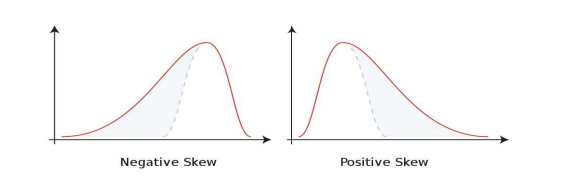
\includegraphics[width=0.6\linewidth]{Figs/C5_1.png}}
	\subfloat[Kurtosis of Distributions]{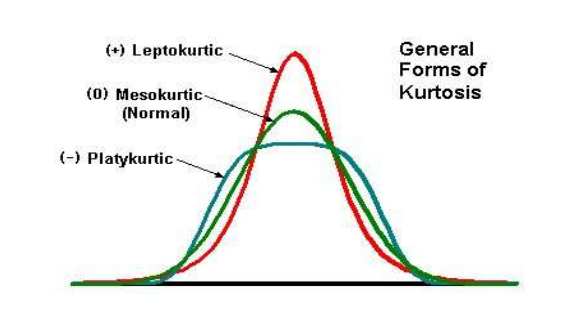
\includegraphics[width=0.4\linewidth]{Figs/C5_2.png}}
    \caption{偏度与峰态}
    \label{fig 5.7.1}
  \end{figure}


\subsection{样本偏度与样本峰度}
根据式 \ref{eq 5.7.1} 和式 \ref{eq 5.7.2} ,用样本三阶矩和四阶矩来计算样本偏度与峰度。样本三阶矩(与样本方差的计算公式相对照)为:
\begin{equation}
     \frac{\sum( \boldsymbol{X-\bar{X}})^{3}}{n-1} 
\end{equation}

样本四阶矩为:
\begin{equation}
    \frac{\sum(\boldsymbol{ X-\bar{X}})^{4}}{n-1}
\end{equation}

前述内容可用于设计正态性的检验。正态分布是对称和常峰态的。对称意味着三阶矩$ \operatorname{E}\boldsymbol{ \varepsilon }^{ 3 } ]$为 0 。分布对称性的标准量是偏态(Skewness)
$$  \sqrt{\beta_{1}}=\frac{\mathbb{E}\left[ \boldsymbol{ \varepsilon }^{3}\right]}{\left(\sigma^{2}\right)^{3 / 2}} $$

峰态(Kurtosis)是分布尾部厚度的度量。此度量是:
$$ \beta_{2}=\frac{\mathbb{E}\left[\boldsymbol{ \varepsilon }^{4}\right]}{\left(\sigma^{2}\right)^{2}} $$

正态分布对于这个度量通常是评价标准;常峰态值是正态分布的峰度,等于 3 。因此,我们可以通过比较偏度是否为 0 和峰度是否为 3 来判断该分布是否为正态分布。在实际中,通常的度量是过量程度(degree of excess)
($ \beta_{2} -3 $) 。我们将使用的工具是一个沃尔德统计量。在正态性的假设下,此检验统计量是:
$$ W=n\left[\frac{b_{1}}{6}+\frac{\left(b_{2}-3\right)^{2}}{24}\right] \sim \chi^{2}(2) $$

称为正态性的哈尔克-贝拉(Jarque-Bera) BJ 检验。

这渐近地服从自由度为 2 的 $ \chi^{2} $分布。这些参数的可行的估计量是利用最小二乘残差计算而得到的。统计量可以参考标准 $ \chi^{2}$表。

由贝拉和哈尔克(1980 a , 1980b )推导的这个检验统计量的皮尔逊分布的内容中是作为拉格朗日乘数检验。应该注意这个检验本质上是无建设性的。非正态性的发现不一定给出
下一步如何做的建议。同样,注意不能拒绝正态性并没有确认了正态性。这只是一个对称性和常峰态的检验。

\section{思考题}

1. 对于线性统计模型 $ \boldsymbol{ y=X \beta+\varepsilon } $。 
假设 $ \varepsilon \sim N\left(0, \sigma^{2} I_{n}\right), n=13, K=3 $,最小化误差平方和 $ \boldsymbol{ (y-X \beta)^{\prime}(y-X \beta)} $
得到如下线性方程组:
$$ \left\{\begin{array}{l}
    b_{1}+2 b_{2}+b_{3} = 3 \\
    2 b_{1}+5 b_{2}+b_{3} = 9 \\
    b_{1}+b_{2}+6 b_{3} = -8
    \end{array}\right. $$
\begin{enumerate}[(1)]
    \item 把这个方程组写成矩阵的形式,并利用矩阵方法求最小二乘估计量$ b $的值。
    \item 如果$ y^{\prime}y = 53 $,求$\sigma^{2} $的无偏估计量 $ s^{2}$ 的值
    \item 求 $ b $ 的协方差矩阵。
    \item 分别写出能够检验 $ H_{0}: \beta_{k}=\beta_{k}^{0} $的 $ t $ 统计量(k=1, 2, 3)。
    \item 写出能够检验$ H_{0}: \beta_{1}+\beta_{2}-2 \beta_{3}=q $ 的 t 统计量和 F 统计量。
\end{enumerate}

2. 假设$ \boldsymbol{ b } $是$ \boldsymbol{ y } $关于$ \boldsymbol{ X } $的回归的最小二乘估计量,$ c $ 是另一$ K \times 1 $向量,证明两个残差平方和之差是:
$$ \boldsymbol{ (y-X c)^{\prime}(y-X c)-(y-X b)^{\prime}(y-X b)=(c-b)^{\prime} X X(c-b)} $$ 

并证明这个差值是正的。

3. 假设对于同一个参数$ \theta $ ,你有两个相互独立的无偏估计量$ \theta^{1} $和$ \theta^{2} $,它们的方差分别为 $ v_{1} $ 和 $ v_{2} $ 且  $ v_{1} \neq v_{1} $  ,
那么什么样的线性组合 $ \hat{\theta}=c_{1} \hat{\theta}_{1}+c_{2} \hat{\theta}_{2} $ 是$ \theta $的最小方差无偏估计量?

4. 假设对于同一个参数$ \theta $ ,你有$ n $个相互独立的无偏估计量 $ \hat{\theta}_{1} \cdots \cdots \hat{\theta}_{n} $,
它们的方差分别 $ v_{1}, \cdots, v_{n} $。那么什么样的线性组合 $ \hat{\theta}=c_{1} \hat{\theta}_{1}+\cdots+c_{n} \hat{\theta}_{n} $是 $ \theta $  的最小方差无偏估计量?
			\chapter{正态线性统计模型的最大似然估计}

\section{最大似然估计}
	我们假定第五章的6个假设条件全部满足,我们就知道了$ \boldsymbol{Y} $的分布函数,
	我们也就可以用其他方法如最大似然估计和矩估计等来求解出参数$ \boldsymbol{ \beta } $和$ \sigma^{2} $的估计量。
	在本章中我们用最大似然估计求出参数$ \boldsymbol{ \beta } $和$ \sigma^{2} $的估计量。

	利用模型的假设和样本信息,我们首先求出\textbf{似然函数},它是关于未知数$ \boldsymbol{\beta} $和$ \sigma^{2} $的函数。
	由于$ \varepsilon \sim N\left(0, \sigma^{2} \boldsymbol{I_{n}} \right) $,
	因此有$ \boldsymbol{y} \sim N \left(\boldsymbol{X \beta}, \sigma^{2} \boldsymbol{I_{n}}\right) $或者
	边际分布$ y_{t} \sim N\left( \boldsymbol{x_{t}^{\prime} \beta}, \sigma^{2}\right) $,
	这里$ \boldsymbol{x_{t}^{\prime}} = \left(x_{t 1}, x_{t 2}, \Lambda, x_{t K}\right), t=1,2, \cdots, n $,
    $ \bm{\{y_{t}\}}$\textbf{是相互独立的(Why?)}。$y_{t}$的密度函数为
	\[f \left(y_{t} \mid \boldsymbol{\beta}, \sigma^{2}\right)
			=\left(2 \pi \sigma^{2}\right)^{-\frac{1}{2}} \exp 
			\left\{-\frac{\left(\boldsymbol{y_{t}-x_{t}^{\prime} \beta}\right)^{2}}{2 \sigma^{2}}\right\}\]
	
    所以$ y_{1}, y_{2}, \cdots, y_{n} $的联合概率密度函数为
	\begin{equation}
		\begin{aligned}
			f\left(y_{t} \mid \boldsymbol{\beta}, \sigma^{2}\right)  
			& =  \left(2 \pi \sigma^{2}\right)^{-\frac{n}{2}} \exp \left\{-\sum_{t=1}^{n} 
				\frac{\left( \boldsymbol{y_{t}-x_{t}^{\prime} \beta}\right)^{2}}{2 \sigma^{2}}\right\} \\
			& =  \left(2 \pi \sigma^{2}\right)^{-\frac{n}{2}} \exp 
			\left \{-\frac{\boldsymbol{(y-X \beta)^{\prime}(y-X \beta)}}{2 \sigma^{2}}\right\} 
		\end{aligned}
	\end{equation}
	
   如果$ y_{1}, y_{2}, \cdots, y_{n} $的联合概率密度函数看做是未知参数
   	$ \boldsymbol{\beta} $和$ \sigma^{2} $的函数,我们称它为\textbf{似然函数},记为   
	\[l\left(\boldsymbol{\beta}, \sigma^{2} \mid \boldsymbol{y} \right)=
		\left(2 \pi \sigma^{2}\right)^{-\frac{n}{2}} \exp 
		\left\{-\frac{\boldsymbol{(y-X \beta)^{\prime}(y-X \beta)}}{2 \sigma^{2}}\right\}\]
	
  \section{最优化问题}
	据最大似然法则,估计未知参数$ \boldsymbol{\beta} $和$ \sigma^{2} $的问题
	变成了选择$ \boldsymbol{\beta} $和$ \sigma^{2} $的值使得对数似然函数的值达到最大,也即是如下的最优化问题:
	$$ \max_{ \boldsymbol{\beta} , \sigma^{2}}  \ \ L \left( \boldsymbol{\beta}, \sigma^{2} \mid \boldsymbol{y} \right) $$
	
  这个问题的一阶条件为
	\begin{equation}
		\begin{aligned}
			\frac{\partial L}{\partial \boldsymbol{\beta} } 
				& =  -\frac{1}{2 \sigma^{2}}\left[\frac{\partial \boldsymbol{(y-X \beta)^{\prime}(y-X \beta)}}{\partial \boldsymbol{\beta}}\right]
				= - \frac{1}{2 \sigma^{2}} \left(-2 \boldsymbol{X^{\prime} y}+2 \boldsymbol{X^{\prime} X \beta}\right)=0 \\
				\frac{\partial L}{\partial \sigma^{2}} 
				& =  -\frac{n}{2} \frac{1}{\sigma^{2}}+\frac{\boldsymbol{(y-X \beta)^{\prime}(y-X \beta)}}{2 \sigma^{4}}=0 
		\end{aligned}
	\end{equation}

    如果把这两个方程的解分别记为$ \hat{\beta} $和$ \hat{\sigma}^{2} $,那么它们满足
	$$ \boldsymbol{ X^{\prime} X \hat{\beta}=X^{\prime} y } $$
	$$  \tilde{\sigma}^{2} = \boldsymbol{\frac{(y-X \hat{\beta})^{\prime}(y-X \hat{\beta})}{n} } $$
	
	可以解得
	\begin{eqnarray}
		\boldsymbol{\hat{\beta}} & = & \boldsymbol{\left(X^{\prime} X\right)^{-1} X^{\prime} y=b} \text{ (与最小二乘估计量一样) } \\
		\hat{\sigma}^{2} & = & \frac{ \boldsymbol{y^{\prime} M y} }{n}
	\end{eqnarray}

	这里$ \boldsymbol{M = I_{n} - X\left ( X^{\prime}  X \right )^{-1}X^{\prime }} $。所以$ \boldsymbol{\beta} $的最大似然估计和最小二乘估计是一样的。
	这是由于选择$ \boldsymbol{\beta} $的值最大化对数似然函数和最小化误差平方和
	$ \boldsymbol{\left ( y - X \beta \right)^{\prime} \left ( y - X \beta \right )} $是等价的。如果记
	$$ \boldsymbol{\hat{e} = y - X \hat{\beta} = My} $$

	并称它为\textbf{最大似然残差},那么它和最小二乘残差是相等的,即$ \boldsymbol{\hat{e} = e = y - X b} $。
	这样$ \sigma^{2} $可表示为$ \hat{\sigma}^{2} = \dfrac{ \boldsymbol{y^{\prime}My} }{n} 
			 = \dfrac{ \boldsymbol{\hat{e}^{\prime}\hat{e}} }{n} 
			 = \dfrac{e^{\prime}e}{n} $

	对于$ \tilde{\boldsymbol{\beta}} $,我们已经知道$ \mathbb{E}\left [ \boldsymbol{\hat{\beta}} \right ] = \boldsymbol{\beta} $,
	$ \operatorname{cor} \left ( \boldsymbol{\hat{\beta}} \right ) = \sigma^{2}\left ( \boldsymbol{X^{\prime}X} \right )^{-1} $。
	由于$ \hat{\beta} = \left ( \boldsymbol{X^{\prime}X} \right )^{-1} \boldsymbol{X^{\prime}y=b} $是$ \boldsymbol{y} $的线性函数,而$ \boldsymbol{y} $服从正态分布,所以
	$ \tilde{\boldsymbol{\beta}} $也服从正态分布,均值为$ \boldsymbol{\beta} $,协方差矩阵为$ \sigma^{2}\left ( \boldsymbol{X^{\prime}X} \right )^{-1} $,
	也即$ \boldsymbol{\hat{\beta}} \sim N \left ( \boldsymbol{\beta}, \sigma^{2}
	\left ( \boldsymbol{X^{\prime}X} \right )^{-1} \right ) $。这个结果在进行区间估计和假设检验时是非常有用的。
	
	关于$ \hat{\sigma}^{2} $,由于$ \mathbb{E} \left [ \boldsymbol{\hat{e}^{\prime}\hat{e}} \right ] 
	= \mathbb{E}\left [ \left ( \boldsymbol{y - X \hat{\beta}} \right)^{\prime} 
	\left ( \boldsymbol{y - X \hat{\beta}} \right ) \right ] 
	= \mathbb{E}\left [ \boldsymbol{\varepsilon^{\prime} M \varepsilon} \right ] 
	= \sigma^{2} \left ( n - K \right ) $,所以其期望值为
	$$ \mathbb{E} \left [ \hat{\sigma}^{2} \right ] = \frac{n - K}{n} \sigma_{2} $$
	
	它是$ \sigma^{2} $的一个有偏估计量,\textbf{其偏度为}\bm{$ -K \sigma_{2} / n $}。为了得到一个无偏估计量,定义
	$$ s^{2} = \frac{ \boldsymbol{\hat{e}^{\prime}\hat{e}}}{n - K} $$
	
	那么它是$ \sigma^{2} $的一个无偏估计量。它和我们在前一章里得到的关于$ \sigma^{2} $的无偏估计量是一样的。
			\chapter{带有线性约束的多元线性回归模型及其假设检验}
	
	在本章中,继续讨论第五章的模型,但新的模型中,参数$ \boldsymbol{\beta} $满足$ J $个线性约束集,$ \boldsymbol{R}\boldsymbol{\beta} = \boldsymbol{q} $,矩阵$ \boldsymbol{R} $有和$ \boldsymbol{\beta} $相一致的$ K $列和总共$ J $个约束的$ J $行,且$ \boldsymbol{R} $是行满秩的,我们考虑不是过度约束的情况,因此,$ J<K $。
	 
	带有线性约束的参数的假设检验,我们可以用两种方法来处理:
	 
	第一个方法是我们按照无约束条件求出一组参数估计后,然后我们对求出的这组参数是否满足假设所暗示的约束,进行检验,我们在本章的第一节中讨论。
	 
	第二个方法是我们把参数所满足的线性约束和模型一起考虑,求出参数的最小二乘解,尔后再作检验,后者就是参数带有约束的最小二乘估计方法,我们在本章的第二节中讨论。
	\section{线性约束的检验}
	从线性回归模型开始,
	\begin{align}
		\boldsymbol{y} = \boldsymbol{X \beta}+\boldsymbol{\varepsilon}
	\end{align}
	我们考虑具有如下形式的一组线性约束,
	\vspace{-0.5em}
	\begin{eqnarray*}
		r_{11} \beta_{1}+r_{12} \beta_{2}+\cdots+r_{1 K} \beta_{K} & = & q_{1} \\
		r_{21} \beta_{1}+r_{22} \beta_{2}+\cdots+r_{2 K} \beta_{K} & = & q_{2} \\
		& \vdots & \\
		r_{J 1} \beta_{1}+r_{J 2} \beta_{2}+\cdots+r_{J K} \beta_{K} & = & q_{J}
	\end{eqnarray*}
	这些可以用矩阵改写成一个方程
	\begin{align}
		\boldsymbol{R \beta} = \boldsymbol{q}	
	\end{align}
	作为我们的假设条件$ H_{0} $。
	
	$ \boldsymbol{R} $中每一行都是一个约束中的系数。矩阵$ \boldsymbol{R} $有和$ \boldsymbol{\beta} $相一致的$ K $列和总共$ J $个约束的$ J $行,且$ \boldsymbol{R} $是行满秩的。因此,$ J $一定要小于或等于$ K $。$ \boldsymbol{R} $的各行必须是线性无关的,虽然$ J = K $的情况并不违反条件,但其唯一决定了$ \boldsymbol{\beta} $,这样的约束没有意义,我们不考虑这种情况。
	
	给定最小二乘估计量$ \boldsymbol{b} $,我们的兴趣集中于“差异”向量$ \boldsymbol{d} = \boldsymbol{Rb}-\boldsymbol{q} $。$ \boldsymbol{d} $精确等于$ \boldsymbol{0} $是不可能的事件(因为其概率是0),统计问题是$ \boldsymbol{d} $对$ \boldsymbol{0} $的离差是否可归因于抽样误差或它是否是显著的。
	
	由于$ \boldsymbol{b} $是多元正态分布的,且$ \boldsymbol{d} $是$ \boldsymbol{b} $的一个线性函数,所以$ \boldsymbol{d} $也是多元正态分布的,若原假设为真,$ \boldsymbol{d} $的均值为0,方差为
	\begin{align}
	var\left [ \boldsymbol{d} \right ] = var\left [ \boldsymbol{Rb-q} \right ] = \boldsymbol{R}\left ( var\left [ \boldsymbol{d} \right ]  \right )
	\boldsymbol{R}^{\prime} = \sigma^{2}\boldsymbol{R}\left ( \boldsymbol{X}^{\prime}\boldsymbol{X} \right )^{-1}\boldsymbol{R}^{\prime} 
	\end{align}
	对$ H_{0} $的检验我们可以将其基于沃尔德(Wald)准则: 
	\begin{equation}
		\begin{aligned}
			W & = \chi^{2}\left ( J \right ) \\
	      	  & = \boldsymbol{d}^{\prime}\left(Var\left [ \boldsymbol{d} \right] \right )
		      ^{-1} \boldsymbol{d} \\
		  	  & = \left ( \boldsymbol{Rb}-\boldsymbol{q} \right )^{\prime}\left [ \sigma^{2}
		      \boldsymbol{R} \left ( \boldsymbol{X}^{\prime}\boldsymbol{X} \right )^{-1}
		      \boldsymbol{R}^{\prime} \right ]^{-1}\left ( \boldsymbol{Rb}-\boldsymbol{q} \right ) \\
		\end{aligned}
		\label{eq 7_1_4}
	\end{equation}
	在假设正确时将服从自由度为\bm{$ J $}的$ \chi^{2} $分布。
	
	直觉上,$ \boldsymbol{d} $越大,即最小二乘满足约束的错误越大,$ \chi^{2} $统计量越大,所以,一个大的
	$ \chi^{2} $值将加重对假设的怀疑。
	\begin{align}
		\frac{(n-K)s^{2}}{\sigma^{2}} = \frac{\boldsymbol{e}^{\prime} \boldsymbol{e}}{\sigma^{2}} = \left(\frac{\boldsymbol{\varepsilon}}
		{\sigma}\right)^{\prime} \boldsymbol{M}\left(\frac{\boldsymbol{\varepsilon}}
		{\sigma}\right)
		\label{eq 7_1_5} 
	\end{align}

	由于$ \sigma $未知,\ref{eq 7_1_4} 中的统计量是不可用的,用$ s^{2} $替代$ \sigma^{2} $,我们可以导出一个$ F\left [ J,\left ( n - K \right )  \right ] $样本统计量,令
	\begin{align}
		F=\frac{(\boldsymbol{R b}-\boldsymbol{q})^{\prime}\left[\sigma^{2} \boldsymbol{R}\left(\boldsymbol{X^{\prime} X}\right)^{-1} \boldsymbol{R}^{\prime}\right]^{-1}(\boldsymbol{R b}-\boldsymbol{q}) / J}{\left[(n-K) s^{2} / \sigma^{2}\right] /(n-K)}
		\label{eq 7_1_6} 
	\end{align}

	分子是$ \left ( 1/J \right )  $乘 \ref{eq 7_1_4} 中的$ W $,分母是$ 1 /\left ( n-K \right ) $乘 \ref{eq 7_1_5}  中的幂等二次型。所以,$ F $是两个除以其自由度的卡方变量的比率。如果它们是独立的,则$ F $的分布是$ F\left [ J,\left (n - K\right ) \right ] $,我们前边发现$ \boldsymbol{b} $是独立于$ s^{2} $分布的,所以条件是满足的。
	
	我们也可以直接推导。利用 \ref{eq 7_1_5} 及$ \boldsymbol{M} $是幂等的这一事实,我们可以把$ F $写为
	\begin{align}
		F=\frac{\{\boldsymbol{R}(\boldsymbol{b}-\boldsymbol{\beta}) / \sigma\}^{\prime}\left[\boldsymbol{R}\left(\boldsymbol{X^{\prime} X}\right)^{-1} \boldsymbol{R}^{\prime}\right]^{-1}\{\boldsymbol{R}(\boldsymbol{b}-\boldsymbol{\beta}) / \sigma\} / J}{[\boldsymbol{M}(\boldsymbol{\varepsilon} / \sigma)]^{\prime}[\boldsymbol{M}(\boldsymbol{\varepsilon} / \sigma)] /(n-K)}
	\end{align}

	由于
	$$\frac{\{\boldsymbol{R}(\boldsymbol{b}-\boldsymbol{\beta})}{\sigma}=\boldsymbol{R}
	\left(\boldsymbol{X^{\prime} X}\right)^{-1} \boldsymbol{X}^{\prime}
	\left(\frac{\boldsymbol{\varepsilon}}{\sigma}\right)=\boldsymbol{T}\left(\frac{\boldsymbol{\varepsilon}}{\sigma}\right) $$

	$ F $统计量是$ \left ( \boldsymbol{\varepsilon} / \sigma\right ) $的两个二次型的比率,由于$ \boldsymbol{M}(\boldsymbol{\varepsilon} / \sigma) $和$ \boldsymbol{T}(\boldsymbol{\varepsilon} / \sigma) $都服从正态分布且它们的协方差$ \boldsymbol{TM} $为$ \boldsymbol{0} $,所以二次型的向量都是独立的。$ F $的分子和分母都是独立随机向量的函数,因而它们也是独立的。这就完成了证明。
	
	消掉 \ref{eq 7_1_6} 中的两个$ \sigma^{2} $,剩下的是检验一个线性假设的$ F $统计量,
	\begin{equation}
		\begin{aligned}
			F & = \frac{(\boldsymbol{Rb}-\boldsymbol{q})^{\prime}\left[\boldsymbol{R}
				\left(\boldsymbol{X^{\prime} X}\right)^{-1} \boldsymbol{R}^{\prime}\right]^{-1}(\boldsymbol{Rb}-\boldsymbol{q}) / J}{\boldsymbol{e}^{\prime} \boldsymbol{e} /(n-K)} \\
			  & = \frac{(\boldsymbol{Rb}-\boldsymbol{q})^{\prime}\left[s^{2} \boldsymbol{R}\left(\boldsymbol{X^{\prime} X}\right)^{-1} \boldsymbol{R}^{\prime}\right]^{-1}(\boldsymbol{Rb}-\boldsymbol{q})}{J}
		\end{aligned}
	\end{equation}

	我们将检验统计量
	$$ F[J, n-K]
	=\frac{(\boldsymbol{Rb}-\boldsymbol{q})^{\prime}\left\{\boldsymbol{R}\left[s^{2}\left(\boldsymbol{X}^{\prime} \boldsymbol{X}\right)^{-1}\right] \boldsymbol{R}^{\prime}\right\}^{-1}(\boldsymbol{Rb}-\boldsymbol{q})}{J} $$
	和$ F $分布表中的临界值相比较,一个大的$ F $值是反对假设的证据。		
	
	注意:将wald统计量中的$ \sigma^{2} $用$ s^{2} $去替代,相应的就将$ J $维的卡方分布转换为维度为$ \left ( J,n-K \right ) $的$ F $分布。
	
	\section{参数带有约束的最小二乘估计}
	\subsection{带有约束的最小二乘函数}
	在许多问题中,要求其中的未知参数$ \boldsymbol{\beta} $满足某特定的线性约束条件:$ \boldsymbol{R\beta}=\boldsymbol{q} $,这里$ \boldsymbol{R} $是$ J\times K $矩阵($ J< K $),并假定它的秩为$ J $维向量,常常希望求$ \boldsymbol{\beta} $的估计$ \hat{\boldsymbol{\beta}} $,使得
	\begin{align}
		\|\boldsymbol{Y}-\boldsymbol{X} \hat{\boldsymbol{\beta}}\|^{2}=\min _{\{\boldsymbol{\beta}: \boldsymbol{R \beta}=\boldsymbol{q}\}}\|\boldsymbol{Y}-\boldsymbol{X \beta}\|^{2}
		\label{eq 7_2_1} 
	\end{align}
	满足条件\ref{eq 7_1_5} 的称为$ \boldsymbol{\beta} $的具有线性约束$ \boldsymbol{R\beta}=\boldsymbol{q} $的最小二乘估计。
	
	解$ \boldsymbol{\hat{\beta}} $的问题实际上是在约束条件
	$$ \boldsymbol{R\beta}=\boldsymbol{q} $$

	下求
	$$ f=\|\boldsymbol{Y}-\boldsymbol{X \beta}\|^{2}=\sum_{i=1}^{n}\left(Y_{i}-\sum_{j=1}^{m} x_{i j} \beta_{j}\right)^{2} $$
	的限制极值点问题。

	这个问题的一个拉格朗日解可写作
	$$ S^{*}=(\boldsymbol{y}-\boldsymbol{X \beta})^{\prime}(\boldsymbol{y}-\boldsymbol{X \beta})+2 \boldsymbol{\lambda}^{\prime}(\boldsymbol{R \beta}-\boldsymbol{q}) $$
	解$ \boldsymbol{b}_{*} $和$ \boldsymbol{\lambda} $将满足必要条件
	\vspace{-0.5em}
	\begin{align*}
		\frac{\partial S^{*}}{\partial \boldsymbol{\beta}} & =  -2 \boldsymbol{X}^{\prime}\left(\boldsymbol{y}-\boldsymbol{X}\boldsymbol{b}_{*}\right)+2 \boldsymbol{R}^{\prime} \boldsymbol{\lambda}=\boldsymbol{0} \\
		\frac{\partial S^{*}}{\partial \boldsymbol{\lambda}} & =  2\left(\boldsymbol{R} \boldsymbol{b}_{*}-\boldsymbol{q}\right)=\boldsymbol{0}
	\end{align*}

	展开可以得到分块矩阵方程
	\begin{equation}
		\left[\begin{array}{lll}
			\boldsymbol{X}^{\prime} \boldsymbol{X} & \boldsymbol{R}^{\prime}  \\
			\boldsymbol{R} & \boldsymbol{0}
		\end{array}\right]\left[\begin{array}{l}
			\boldsymbol{b}_{*} \\
			\boldsymbol{\lambda}
		\end{array}\right]=\left[\begin{array}{l}
			\boldsymbol{X}^{\prime} \boldsymbol{y} \\
			\boldsymbol{q}
		\end{array}\right]
	\end{equation}

	或
	$$ \boldsymbol{Wd}_{*}=\boldsymbol{v} $$

	假定括号中的分块矩阵是非奇异的,约束最小二乘估计量
	\begin{equation}
		\begin{aligned}
			\boldsymbol{d}_{*} & = \boldsymbol{W}^{-1}\boldsymbol{v} = \left[\begin{array}{l} \boldsymbol{b}_{*} \\ 
			\boldsymbol{\lambda}
			\end{array}\right]
		\end{aligned}
	\end{equation}

	其中
	$$  \boldsymbol{W}^{-1}=\left[ \begin{array}{cc}
			\left( \boldsymbol{X}^{\prime} \boldsymbol{X}\right)^{-1}-
			\left(\boldsymbol{X}^{\prime} \boldsymbol{X}\right)^{-1} 
			\boldsymbol{R}^{\prime}
			 \left(\boldsymbol{R}\left(\boldsymbol{X}^{\prime} \boldsymbol{X}\right)^{-1} \boldsymbol{R}^{\prime}\right)^{-1} \boldsymbol{R}\left(\boldsymbol{X}^{\prime} \boldsymbol{X}\right)^{-1} & 
			 \left(\boldsymbol{X}^{\prime} \boldsymbol{X}\right)^{-1} 
			 \boldsymbol{R}^{\prime}\left(\boldsymbol{R}
			 \left(\boldsymbol{X}^{\prime} 
			 \boldsymbol{X}\right)^{-1} \boldsymbol{R}^{\prime}\right)^{-1} \\
			\left(\boldsymbol{R}\left(\boldsymbol{X}^{\prime} \boldsymbol{X}\right)^{-1} \boldsymbol{R}^{\prime}\right)^{-1} 
			\boldsymbol{R}\left(\boldsymbol{X}^{\prime} \boldsymbol{X}\right)^{-1} & -
			\left(\boldsymbol{R}\left(\boldsymbol{X}^{\prime} \boldsymbol{X}\right)^{-1} \boldsymbol{}\boldsymbol{R}^{\prime}\right)^{-1}
	\end{array}\right] $$

	的解。此外,若$ \boldsymbol{X}^{\prime} \boldsymbol{X} $是非奇异的,则用分块逆公式可以得到$ \boldsymbol{b}_{*} $和$ \boldsymbol{\lambda} $的显示解
	{ \small
		\begin{equation}
			% \small
			\begin{aligned}
				\boldsymbol{b}_{*} & = \left(\boldsymbol{X}^{\prime} \boldsymbol{X}\right)^{-1} \boldsymbol{X}^{\prime} \boldsymbol{y}-\left(\boldsymbol{X}^{\prime} \boldsymbol{X}\right)^{-1} \boldsymbol{R}^{\prime}\left(\boldsymbol{R}\left(\boldsymbol{X}^{\prime} \boldsymbol{X}\right)^{-1} \boldsymbol{R}^{\prime}\right)^{-1} \boldsymbol{R}\left(\boldsymbol{X}^{\prime} \boldsymbol{X}\right)^{-1} \boldsymbol{X}^{\prime} \boldsymbol{y}+\left(\boldsymbol{X}^{\prime} \boldsymbol{X}\right)^{-1} \boldsymbol{R}^{\prime}\left(\boldsymbol{R}\left(\boldsymbol{X}^{\prime} X\right)^{-1} \boldsymbol{R}^{\prime}\right)^{-1} \boldsymbol{q} \\
				& = \left(\boldsymbol{X}^{\prime} \boldsymbol{X}\right)^{-1} \boldsymbol{X}^{\prime} \boldsymbol{y}-\left(\boldsymbol{X}^{\prime} \boldsymbol{X}\right)^{-1} \boldsymbol{R}^{\prime}\left(\boldsymbol{R}\left(\boldsymbol{X}^{\prime} \boldsymbol{X}\right)^{-1} \boldsymbol{R}^{\prime}\right)^{-1} \boldsymbol{R}\left(\boldsymbol{X}^{\prime} \boldsymbol{X}\right)^{-1} \boldsymbol{X}^{\prime}(\boldsymbol{X }\boldsymbol{b}+\boldsymbol{e})+\left(\boldsymbol{X}^{\prime} \boldsymbol{X}\right)^{-1} \boldsymbol{R}^{\prime}\left(\boldsymbol{R}\left(\boldsymbol{X}^{\prime} \boldsymbol{X}\right)^{-1} \boldsymbol{R}^{\prime}\right)^{-1} \boldsymbol{q} \\
				& = \left(\boldsymbol{X}^{\prime} \boldsymbol{X}\right)^{-1} \boldsymbol{X}^{\prime} \boldsymbol{y}-\left(\boldsymbol{X}^{\prime} \boldsymbol{X}\right)^{-1} \boldsymbol{R}^{\prime}\left(\boldsymbol{R}\left(\boldsymbol{X}^{\prime} \boldsymbol{X}\right)^{-1} \boldsymbol{R}^{\prime}\right)^{-1} \boldsymbol{R} \boldsymbol{b}+\left(\boldsymbol{X}^{\prime} \boldsymbol{X}\right)^{-1} \boldsymbol{R}^{\prime}\left(\boldsymbol{R}\left(\boldsymbol{X}^{\prime} \boldsymbol{X}\right)^{-1} \boldsymbol{R}^{\prime}\right)^{-1} \boldsymbol{q} \\
				& = \boldsymbol{b}-\left(\boldsymbol{X}^{\prime} \boldsymbol{X}\right)^{-1} \boldsymbol{R}^{\prime}\left[\boldsymbol{R}\left(\boldsymbol{X}^{\prime} \boldsymbol{X}\right)^{-1} \boldsymbol{R}^{\prime}\right]^{-1}(\boldsymbol{R b}-\boldsymbol{q}) \nonumber
			\end{aligned}
		\end{equation} 
	}

	和
		$$ \boldsymbol{\lambda}=\left[\boldsymbol{R}\left(\boldsymbol{X}^{\prime} \boldsymbol{X}\right)^{-1} 
		\boldsymbol{R}^{\prime}\right]^{-1}(\boldsymbol{R b}-\boldsymbol{q}) $$

	格林和西克斯(1991)表明$ \boldsymbol{b}_{*} $的协方差矩阵简单地就是$ \sigma^{2} $乘以$ W^{-1} $
	的左上块,在$ \boldsymbol{X}^{\prime} \boldsymbol{X} $非奇异的通常情况下,再一次可以得到一个显性公式
	$$ \operatorname{Var}\left[\boldsymbol{b}_{*}\right]=\sigma^{2}\left(\boldsymbol{X}^{\prime} \boldsymbol{X}\right)^{-1}-\sigma^{2}\left(\boldsymbol{X}^{\prime} \boldsymbol{X}\right)^{-1} \boldsymbol{R}^{\prime}\left[\boldsymbol{R}\left(\boldsymbol{X}^{\prime} \boldsymbol{X}\right)^{-1} \boldsymbol{R}^{\prime}\right]^{-1} \boldsymbol{R}\left(\boldsymbol{X}^{\prime} \boldsymbol{X}\right)^{-1} $$

	这样,
	$$ \operatorname{Var}\left[\boldsymbol{b}_{*}\right]=\operatorname{Var}[\boldsymbol{b}]-\ \ (\text {一个非负定矩阵 }) $$

	$ \operatorname{Var}\left[\boldsymbol{b}_{*}\right] $的方差比$ \operatorname{Var}[\boldsymbol{b}] $小的一个解释是约束条件提供了更多的信息价值。
	\subsection{对约束的检验的另一个方法}
	令$ \boldsymbol{e}_{*}=\boldsymbol{y}-\boldsymbol{X b}_{*} $,我们来计算新的离差平方和$ \boldsymbol{e}_{*}^{\prime} \boldsymbol{e}_{*} $。
	$$ \boldsymbol{e}_{*}=\boldsymbol{y}-\boldsymbol{Xb}-\boldsymbol{X}\left(\boldsymbol{b}_{*}-\boldsymbol{b}\right)=\boldsymbol{e}-\boldsymbol{X}\left(\boldsymbol{b}_{*}-\boldsymbol{b}\right) $$
	
	则新的离差平方和是
	$$ \boldsymbol{e}_{*}^{\prime} \boldsymbol{e}_{*}=\boldsymbol{e}^{\prime} \boldsymbol{e}+\left(\boldsymbol{b}_{*}-\boldsymbol{b}\right)^{\prime} \boldsymbol{X}^{\prime} \boldsymbol{X}\left(\boldsymbol{b}_{*}-\boldsymbol{b}\right) \geq \boldsymbol{e}^{\prime} \boldsymbol{e} $$

	其中,
	$$ \frac{\boldsymbol{e}^{\prime} \boldsymbol{e}}{\sigma^{2}} \sim \chi_{n-k}^{2}\quad \frac{\boldsymbol{e}_{*}^{\prime} \boldsymbol{e}_{*}}{\sigma^{2}} \sim \chi_{n-(k-J)}^{2}  $$

	因为新的模型中参数的个数为$ k-J $个,$ J $个榆树条件是原模型中的$ J $个参数可以被其他$ k-J $个表示。(此表达式中的中间项含有$ \boldsymbol{X}^{\prime} \boldsymbol{e} $,它是$ \boldsymbol{0} $)。这说明我们可以将一个约束检验基于拟合的损失。这个损失是,
	$$ \boldsymbol{e}_{*}^{\prime} \boldsymbol{e}_{*}-\boldsymbol{e}^{\prime} \boldsymbol{e}=(\boldsymbol{Rb}-\boldsymbol{q})^{\prime}\left[\boldsymbol{R}\left(\boldsymbol{X}^{\prime} \boldsymbol{X}\right)^{-1} \boldsymbol{R}^{\prime}\right]^{-1}(\boldsymbol{Rb}-\boldsymbol{q}) $$

	这出现在前边推导的$ F $统计量的分子上,我们得到统计量的另一个可选形式。可选形式是
		$$ F[J, n-K]=\frac{\left(\boldsymbol{e}_{*}^{\prime} \boldsymbol{e}_{*}-\boldsymbol{e}^{\prime} 
		\boldsymbol{e}\right) / J}{\boldsymbol{e}^{\prime} \boldsymbol{e} /(n-K)} $$

	最后,以$ \mathrm{SST}=\Sigma(y-\bar{y})^{2} $除$ F $的分子和分母,我们得到第三种形式,
	$$ F[J, n-K]=\frac{\left(R^{2}-R_{*}^{2}\right) / J}{\left(1-R^{2}\right) /(n-K)} $$
	
	由于两个模型的拟合之差直接体现在检验统计量中,这个形式具有一些直观吸引力。
	\subsection{实例}
	所有柯布—道格拉斯模型的一般化是如下的对数变换模型,
	\begin{align}
		\log Y = \beta_{1}+\beta_{2} \log L+\beta_{3} \log K+\beta_{4} \frac{\log ^{2} L}{2}+\beta_{5} \frac{\log ^{2} K}{2}+\beta_{6} \frac{\log L \log K}{2}+\varepsilon
	\end{align}

	无约束回归的结果在表\ref{tab 7.1}中给出。
	\begin{table}[htbp]
		\centering
		\setlength{\tabcolsep}{3em}
		\caption{无约束回归的结果}
		\begin{tabular}{ll}
		\hline
			回归标准误差 & 0.17994 \\
			残差平方和  & 0.67993 \\
			R平方    & 0.95486 \\
			调整R平方  & 0.94411 \\
		\hline
		\end{tabular}
		\label{tab 7.1}
	\end{table}

	\begin{table}[htbp]
		\centering
		\setlength{\tabcolsep}{3em}
		\caption{无约束回归的系数结果}
		\begin{tabular}{llll}
			\hline
			变量   & 系数       & 标准误差   & t值     \\
			\hline
			常数项  & 0.944216 & 2.911  & 0.324  \\
			$ \log L $ & 3.61363  & 1.548  & 2.334  \\
			$ \log K $ & -1.89311 & 1.016  & -1.863 \\
			$ \frac{1}{2}\log^{2}L $ & -0.96406 & 0.7074 & -1.363 \\
			$ \frac{1}{2}\log^{2}K $ & 0.08529  & 0.2926 & 0.291  \\
			$ \log L \times \log K $ & 0.31239  & 0.4389 & 0.71  \\
			\hline
		\end{tabular}
	\end{table}
	\begin{table}[htbp]
		\centering
		\caption{系数估计量的估计协方差矩阵}
		\begin{tabular}{llllccc}
			\hline
			& 常数项  & $ \log L $  & $ \log K $  & $ \frac{1}{2}\log^{2}L $  & $ \frac{1}{2}\log^{2}K $  & $ \log L \times \log K $        \\
			常数项      & 8.472    &         &         &         &         &        \\
			$ \log L $ & -2.388   & 2.397   &         &         &         &        \\
			$ \log K $ & -0.3313  & -1.231  & 1.033   &         &         &        \\
			$ \frac{1}{2}\log^{2}L $ & -0.08760 & -0.6658 & 0.5231  & 0.5004  &         &        \\
			$ \frac{1}{2}\log^{2}K $ & 0.2332   & 0.03477 & 0.02637 & 0.1467  & 0.08562 &        \\
			$ \log L \times \log K $ & 0.3635   & 0.1831  & -0.2255 & -0.2880 & -0.1160 & 0.1927    \\
			\hline
		\end{tabular}
	\end{table}

	考虑了约束条件$ \beta_{4}=\beta_{5}=\beta_{6}=0 $的模型就可以得到柯布一道格拉斯模型:
	$$ \log Y=\beta_{1}+\beta_{2} \log L+\beta_{3} \log K+\varepsilon $$
	
	这是一个条件约束下的无条件的多元线性回归模型。就可以用一般线性回归的方法求解模型。假如我们通过有约束条件下的无条件的多元线性回归模型得到:$ \boldsymbol{e}_{*}^{\prime} \boldsymbol{e}_{*}=0.85163 $,而且$ n-K=21  $,则柯布—道格拉斯模型假设的$ F $统计量是
	$$ F\left [ 3,21 \right ] =\frac{(0.85163-0.67993) / 3}{0.67993 / 21}=1.768 $$

	查自$ F $分布表的$ 5\% $临界值是3.07,所以我们不能拒绝柯布—道格拉斯模型是适当的这一假设。
	
	考虑了约束条件$ \beta_{4}=\beta_{5}=\beta_{6}=0 $和条件$ \beta_{2}+\beta_{3}=1 $的模型就是满足规模效应的柯布—道格拉斯生产函数。这个模型可以推导如下:
	\begin{equation}
		\begin{aligned}
			\log Y & = \beta_{1}+\beta_{2} \log L+\beta_{3} \log K+\varepsilon \\
			       & = \beta_{1}+\beta_{2} \log L+\left(1-\beta_{2}\right) \log K+\varepsilon
		\end{aligned}
	\end{equation}
	$$ \Longrightarrow \log Y-\log L=\beta_{1}+\beta_{2}(\log L-\log K)+\varepsilon $$
	
	假如我们通过有约束条件下的无条件的多元线性回归模型得到:
	$ {\boldsymbol{e}_{*}}^{\prime} \boldsymbol{e}_{*}=0.89172 $,而且$ n-K=21  $,则柯布—道格拉斯模型假设的$ F $统计量是
	$$ F\left [ 4,21 \right ] =\frac{(0.89172-0.67993) / 4}{0.67993 / 21}=1.635 $$
	查自$ F $分布表的$ 5\% $临界值是$ 2.85 $,所以我们不能拒绝柯布—道格拉斯模型是规模效应的生产函数的这一假设。
	
	\section{结构变化与邹至庄检验(Structure Change and Chou-Test)}
	\subsection{问题提出}
	我们经常碰到这样的问题。某项政策的出台及实施,其效果如何?不同地区或不同时期内,我们分别可以得到这两个地区或时期的观测值,我们的问题是:这两个地区或时期的情况是否不同,经济结构有无差异。
	
	这类问题,被华人经济学家邹至庄用构造的$ F $检验解决了(1960年)。这样的$ F $检验的统计量,就称为邹至庄检验( Chou-Test)。
	\subsection{问题的模型表述}
	设$ \left(\boldsymbol{Z}_{1},\boldsymbol{Y}_{1}\right) $,$ \left(\boldsymbol{Z}_{2},\boldsymbol{Y}_{2}\right) $分别表示这两个时期的观测值,允许两个时期中系数不同的无约束回归是
	$$  \left\{\begin{array}{l}
		   \boldsymbol{Y}_{1}=\boldsymbol{Z}_{1} \boldsymbol{\beta}_{1}+\boldsymbol{\varepsilon}_{1} \\
		   \boldsymbol{Y}_{2}=\boldsymbol{Z}_{2} \boldsymbol{\beta}_{2}+\boldsymbol{\varepsilon}_{2}
	\end{array}\right. $$
	我们可以将其改写成一个回归方程:
	\begin{equation}
		\left(\begin{array}{l}
			\boldsymbol{Y}_{1} \\
			\boldsymbol{Y}_{2}
		\end{array}\right)=\left(\begin{array}{cc}
			\boldsymbol{Z}_{1} & \boldsymbol{0} \\
			\boldsymbol{0} & \boldsymbol{Z}_{2}
		\end{array}\right)\left(\begin{array}{c}
			\boldsymbol{\beta}_{1} \\
			\boldsymbol{\beta}_{2}
		\end{array}\right)+\left(\begin{array}{c}
			\boldsymbol{\varepsilon}_{1} \\
			\boldsymbol{\varepsilon}_{2}
		\end{array}\right)
		\label{eq 7_3_1}
	\end{equation}

	即$ \boldsymbol{Y}=\boldsymbol{Z \beta}+\boldsymbol{\varepsilon} $模型,其中
	$$ \boldsymbol{Y}=\left(\begin{array}{l}
		\boldsymbol{Y}_{1} \\
		\boldsymbol{Y}_{2}
	\end{array}\right),
	\boldsymbol{Z}=\left(\begin{array}{cc}
		\boldsymbol{Z}_{1} & \boldsymbol{0} \\
		\boldsymbol{0} & \boldsymbol{Z}_{2}
	\end{array}\right),
	\boldsymbol{\beta}=\left(\begin{array}{l}
		\boldsymbol{\beta}_{1} \\
		\boldsymbol{\beta}_{2}
	\end{array}\right),
	\boldsymbol{\varepsilon}=\left(\begin{array}{c}
		\boldsymbol{\varepsilon}_{1} \\
		\boldsymbol{\varepsilon}_{2}
	\end{array}\right) $$

	上述问题就转换成检验
	$$ \begin{array}{l}
		H_{0}: \boldsymbol{\beta}_{1}=\boldsymbol{\beta}_{2} \\
		H_{1}: \boldsymbol{\beta}_{1} \neq \boldsymbol{\beta}_{2}
	\end{array} $$

	的问题。我们可以用两种方式来处理问题:

		{ \heiti{ 1. }} 用约束条件$ \boldsymbol{\beta}_{1}=\boldsymbol{\beta}_{2} $来检验。
		$ \boldsymbol{\beta}_{1}=\boldsymbol{\beta}_{2} $是更一般约束条件$ \boldsymbol{R\beta}=\boldsymbol{q} $的一个特殊形式,其中$ \boldsymbol{R}=(\boldsymbol{I},-\boldsymbol{I}) $和$ \boldsymbol{q}=\boldsymbol{0} $。这个直接可以从基于{\bf Wald统计量}的带约束条件的$ F $检验得到。(请自己推导)。
		
		\begin{myexample}
			用约束条件下的$ F $ 检验推导出邹至庄检验的表达式。
			\begin{myproof}
				在约束条件$ \boldsymbol{R\beta}=\boldsymbol{q} $下,$ F $检验
					$$ F(J, n-k)=\frac{(\boldsymbol{Rb}-\boldsymbol{q})^{\prime}\left[S^{2} \boldsymbol{R}\left(\boldsymbol{Z}^{\prime} 
					\boldsymbol{Z}\right)^{-1} \boldsymbol{R}^{\prime}\right]^{-1}(\boldsymbol{Rb}-\boldsymbol{q})}{J} $$

					而邹至庄检验时约束条件$ \boldsymbol{R\beta}=\boldsymbol{q} $的一种特殊形式,即$ \boldsymbol{R}=(\boldsymbol{I},-\boldsymbol{I}) $和$ \boldsymbol{q}=\boldsymbol{0} $,也即等同于条件$ \boldsymbol{\beta}_{1}=\boldsymbol{\beta}_{2} $(有$ 2k $个参数,并且是有$ k $个约束)。故
					\begin{align*}
						F\left(k, n_{1}+n_{2}-2 k\right) & =  \dfrac{(\boldsymbol{Rb}-\boldsymbol{q})^{\prime}\left[S^{2} \boldsymbol{R}\left(\boldsymbol{Z}^{\prime} \boldsymbol{Z}\right)^{-1} \boldsymbol{R}^{\prime}\right]^{-1}(\boldsymbol{Rb}-\boldsymbol{q})}{k} \\
						& =  \dfrac{\left(\boldsymbol{b}_{1}-\boldsymbol{b}_{2}\right)^{\prime}\left[S^{2}(\boldsymbol{I},-\boldsymbol{I})\left(\begin{array}{cc}
								\left(\boldsymbol{Z}_{1}^{\prime} \boldsymbol{Z}_{1}\right)^{-1} & \boldsymbol{0} \\
								\boldsymbol{0} & \left(\boldsymbol{Z}_{2}^{\prime} \boldsymbol{Z}_{2}\right)^{-1}
							\end{array}\right)\left(\begin{array}{c}
								\boldsymbol{I} \\
								-\boldsymbol{I}
							\end{array}\right)\right]^{-1}\left(\boldsymbol{b}_{1}-\boldsymbol{b}_{2}\right)}{k} \\
						& =  \dfrac{\left(\boldsymbol{b}_{1}-\boldsymbol{b}_{2}\right)^{\prime}\left[S^{2}\left(\left(\boldsymbol{Z}_{1}^{\prime} \boldsymbol{Z}_{1}\right)^{-1}+\left(\boldsymbol{Z}_{2}^{\prime} \boldsymbol{Z}_{2}\right)^{-1}\right)\right]^{-1}\left(\boldsymbol{b}_{1}-\boldsymbol{b}_{2}\right)}{k}
					\end{align*}

					服从$ F\left(k, n_{1}+n_{2}-2 k\right) $的分布。
			\end{myproof}
		\end{myexample}
		

		% \setlength{\parindent}{2\ccwd}

		
		另外,在考虑了约束条件$ \boldsymbol{\beta}_{1}=\boldsymbol{\beta}_{2} $后,我们可以将模型 \ref{eq 7_3_1} 改写成一个无约束的新的回归方程
		
		$$ \left(
				\begin{array}{l}
					\boldsymbol{Y}_{1} \\
					\boldsymbol{Y}_{2}
				\end{array}\right)		
			=\left(\begin{array}{cc}
				\boldsymbol{Z}_{1} & \boldsymbol{0} \\
				\boldsymbol{0} & \boldsymbol{Z}_{2}
			\end{array}\right)\left(\begin{array}{c}
				\boldsymbol{\beta}_{1} \\
				\boldsymbol{\beta}_{1}
			\end{array}\right)+\left(\begin{array}{c}
				\boldsymbol{\varepsilon}_{1} \\
				\boldsymbol{\varepsilon}_{2}
			\end{array} \right) $$

		即
		\begin{equation}
			\left(\begin{array}{c}
				\boldsymbol{Y}_{1} \\
				\boldsymbol{Y}_{2}
			\end{array}\right)=\left(\begin{array}{c}
				\boldsymbol{Z}_{1} \\
				\boldsymbol{Z}_{2}
			\end{array}\right) \boldsymbol{\beta}_{1}+\left(\begin{array}{c}
				\boldsymbol{\varepsilon}_{1} \\
				\boldsymbol{\varepsilon}_{2}
			\end{array}\right) 
			\label{eq 7_3_2}
		\end{equation}

		即无约束的线性模型即$ \boldsymbol{Y}=\boldsymbol{Z} \boldsymbol{\beta}+\boldsymbol{\varepsilon} $模型,其中
		$$ \boldsymbol{Y}=\left(\begin{array}{l}
			\boldsymbol{Y}_{1} \\
			\boldsymbol{Y}_{2}
		\end{array}\right),
		\boldsymbol{Z}=\left(\begin{array}{cc}
			\boldsymbol{Z}_{1}  \\
			\boldsymbol{Z}_{2}
		\end{array}\right),
		\boldsymbol{\beta} = \boldsymbol{\beta}_{1} = \boldsymbol{\beta}_{2},
		\boldsymbol{\varepsilon}=\left(\begin{array}{c}
			\boldsymbol{\varepsilon}_{1} \\
			\boldsymbol{\varepsilon}_{2}
		\end{array}\right) $$
		
		假如模型 \ref{eq 7_3_2} 的残差平方和是$ \boldsymbol{e}_{*}^{\prime} \boldsymbol{e}_{*} $ ,在假设条件$ \beta_{1}=\beta_{2} $下, 我们可以得到$ F $统计量可更简单地表示为:
		$$ F\left[k, n_{1}+n_{2}-2 k\right]=\frac{\left ( \boldsymbol{e}_{*}^{\prime} \boldsymbol{e}_{*}-\boldsymbol{e}^{\prime} \boldsymbol{e} \right )/k }{\left ( \boldsymbol{e}^{\prime} \boldsymbol{e}  \right )/\left ( n_{1}+n_{2}-2k \right ) } $$

		{\bf{2.}} 更直接、更容易的一个处理是将约束直接构造进模型中。若两个系数向量相同,则模型 \ref{eq 7_3_1} 就转换为 \ref{eq 7_3_3} :
		\begin{equation}
			\left(\begin{array}{c}
				\boldsymbol{Y}_{1} \\
				\boldsymbol{Y}_{2}
			\end{array}\right)=\left(\begin{array}{c}
				\boldsymbol{Z}_{1} \\
				\boldsymbol{Z}_{2}
			\end{array}\right) \boldsymbol{\beta}+\left(\begin{array}{c}
				\boldsymbol{\varepsilon}_{1} \\
				\boldsymbol{\varepsilon}_{2}
			\end{array}\right)
			\label{eq 7_3_3}
		\end{equation}	

		由此我们推导出可以检验的邹至庄统计量Chou-Test。
		
		从模型 \ref{eq 7_3_1}  中,我们可以得到无约束最小二乘估计量是
		\begin{eqnarray*}
			\boldsymbol{b} & = & \left(\boldsymbol{Z}^{\prime} \boldsymbol{Z}\right)^{-1} \boldsymbol{Z}^{\prime} \boldsymbol{Y} \\
			 & = & \left(\begin{array}{cc}
			\boldsymbol{Z}_{1}^{\prime} \boldsymbol{Z}_{1} & \boldsymbol{0} \\
			\boldsymbol{0} & \boldsymbol{Z}_{2}^{\prime} \boldsymbol{Z}_{2}
			\end{array}\right)^{-1}\left(\begin{array}{c}
			\boldsymbol{Z}_{1}^{\prime} \boldsymbol{Y}_{1} \\
			\boldsymbol{Z}_{2}^{\prime} \boldsymbol{Y}_{2} \end{array}\right) \\
		    & = & \left(\begin{array}{cc}
			\left(\boldsymbol{Z}_{1}^{\prime} \boldsymbol{Z}_{1}\right)^{-1} & \boldsymbol{0} \\ 
			\boldsymbol{0} & \left(\boldsymbol{Z}_{2}^{\prime} \boldsymbol{Z}_{2}\right)^{-1}
			\end{array}\right)\left(\begin{array}{c}
			\boldsymbol{Z}_{1}^{\prime} \boldsymbol{Y}_{1} \\
			\boldsymbol{Z}_{2}^{\prime} \boldsymbol{Y}_{2}
			\end{array}\right) \\
		     & = & \left(\begin{array}{c}
			\boldsymbol{b}_{1} \\
			\boldsymbol{b}_{2}
			\end{array}\right)		
		\end{eqnarray*}

		故		
		\begin{eqnarray*}
			\boldsymbol{e}=\boldsymbol{Y}-\boldsymbol{Zb} & = & \left(\begin{array}{c}
				\boldsymbol{Y}_{1} \\
				\boldsymbol{Y}_{2}
			\end{array}\right)-\left(\begin{array}{cc}
				\boldsymbol{Z}_{1} & \boldsymbol{0} \\
				\boldsymbol{0} & \boldsymbol{Z}_{2}
			\end{array}\right)\left(\begin{array}{c}
				\left(\boldsymbol{Z}_{1}^{\prime} \boldsymbol{Z}_{1}\right)^{-1} \boldsymbol{Z}_{1}^{\prime} \boldsymbol{Y}_{1} \\
				\left(\boldsymbol{Z}_{2}^{\prime} \boldsymbol{Z}_{2}\right)^{-1} \boldsymbol{Z}_{2}^{\prime} \boldsymbol{Y}_{2}
			\end{array}\right) \\
			& = & \left(\begin{array}{c}
				\boldsymbol{Y}_{1} \\
				\boldsymbol{Y}_{2}
			\end{array}\right)-\left(\begin{array}{cc}
				\boldsymbol{Z}_{1} & \boldsymbol{0} \\
				\boldsymbol{0} & \boldsymbol{Z}_{2}
			\end{array}\right)\left(\begin{array}{cc}
				\left(\boldsymbol{Z}_{1}^{\prime} \boldsymbol{Z}_{1}\right)^{-1} \boldsymbol{Z}_{1}^{\prime} & \boldsymbol{0} \\
				\boldsymbol{0} & \left(\boldsymbol{Z}_{2}^{\prime} \boldsymbol{Z}_{2}\right)^{-1} \boldsymbol{Z}_{2}^{\prime}
			\end{array}\right)\left(\begin{array}{c}
				\boldsymbol{Y}_{1} \\
				\boldsymbol{Y}_{2}
			\end{array}\right) \\
			& = & \left[\boldsymbol{I}-\left(\begin{array}{cc}
				\boldsymbol{Z}_{1}\left(\boldsymbol{Z}_{1}^{\prime} \boldsymbol{Z}_{1}\right)^{-1} \boldsymbol{Z}_{1}^{\prime} & \boldsymbol{0} \\
				\boldsymbol{0} & \boldsymbol{Z}_{2}\left(\boldsymbol{Z}_{2}^{\prime} \boldsymbol{Z}_{2}\right)^{-1} \boldsymbol{Z}_{2}^{\prime}
			\end{array}\right)
			\left(\begin{array}{c}
				\boldsymbol{Y}_{1} \\
				\boldsymbol{Y}_{2}
			\end{array}\right) \right]=
			\left(\begin{array}{c}
				\boldsymbol{e}_{1} \\
				\boldsymbol{e}_{2}
			\end{array}\right) \\
			& = & \boldsymbol{M}_{1}\left(\begin{array}{l}
				\boldsymbol{Y}_{1} \\
				\boldsymbol{Y}_{2}
			\end{array}\right)
		\end{eqnarray*}

		因此
		$$ \boldsymbol{e}^{\prime} \boldsymbol{e}=\left(\boldsymbol{Y}_{1}^{\prime} \boldsymbol{Y}_{2}^{\prime}\right) \boldsymbol{M}_{1}^{\prime} \boldsymbol{M}_{1}\left(\begin{array}{l}
			\boldsymbol{Y}_{1} \\
			\boldsymbol{Y}_{2}
		\end{array}\right)=\left(\boldsymbol{Y}_{1}^{\prime} \boldsymbol{Y}_{2}^{\prime}\right) \boldsymbol{M}_{1}\left(\begin{array}{l}
			\boldsymbol{Y}_{1} \\
			\boldsymbol{Y}_{2}
		\end{array}\right) $$

		则$ \boldsymbol{e}^{\prime} \boldsymbol{e}/\sigma^{2} \sim \chi^{2}\left(n_{1}+n_{2}-2 k\right) $。
		
		对于有约束条件$ \boldsymbol{\beta}_{1}=\boldsymbol{\beta}_{2} $限制的模型\ref{eq 7_3_3} 
		\begin{eqnarray*}
			\boldsymbol{e}^{*} & = & \left(\boldsymbol{I}-\left(\begin{array}{c}
				\boldsymbol{Z}_{1} \\
				\boldsymbol{Z}_{2}
			\end{array}\right)\left(\left(\boldsymbol{Z}_{1}^{\prime} \boldsymbol{Z}_{2}^{\prime}\right) \cdot\left(\begin{array}{c}
				\boldsymbol{Z}_{1} \\
				\boldsymbol{Z}_{2}
			\end{array}\right)\right)^{-1}\left(\boldsymbol{Z}_{1}^{\prime} \boldsymbol{Z}_{2}^{\prime}\right)\right)\left(\begin{array}{c}
				\boldsymbol{Y}_{1} \\
				\boldsymbol{Y}_{2}
			\end{array}\right) \\
			& = & \left(\boldsymbol{I}-\left(\begin{array}{c}
				\boldsymbol{Z}_{1} \\
				\boldsymbol{Z}_{2}
			\end{array}\right)\left(\boldsymbol{Z}_{1}^{\prime} \boldsymbol{Z}_{1}+\boldsymbol{Z}_{2}^{\prime} \boldsymbol{Z}_{2}\right)^{-1}\left(\boldsymbol{Z}_{1}^{\prime} \boldsymbol{Z}_{2}^{\prime}\right)\right)\left(\begin{array}{c}
				\boldsymbol{Y}_{1} \\
				\boldsymbol{Y}_{2}
			\end{array}\right) \\
			& = & \boldsymbol{M}_{2}\left(\begin{array}{l}
			\boldsymbol{Y}_{1} \\
			\boldsymbol{Y}_{2}
		\end{array}\right)
		\end{eqnarray*}

		因此
		$$ \boldsymbol{e}^{* \prime} \boldsymbol{e}^{*}=\left(\boldsymbol{Y}_{1}^{\prime} \boldsymbol{Y}_{2}^{\prime}\right) \boldsymbol{M}_{2}^{\prime} \boldsymbol{M}_{2}\left(\begin{array}{c}
			\boldsymbol{Y}_{1} \\
			\boldsymbol{Y}_{2}
		\end{array}\right)=\left(\boldsymbol{Y}_{1}^{\prime} \boldsymbol{Y}_{2}^{\prime}\right) \boldsymbol{M}_{2}\left(\begin{array}{c}
			\boldsymbol{Y}_{1} \\
			\boldsymbol{Y}_{2}
		\end{array}\right) $$

		则$ \boldsymbol{e}^{*\prime} \boldsymbol{e}^{*}/\sigma^{2} \sim \chi^{2}\left(n_{1}+n_{2}-k\right) $。
		$$ \boldsymbol{e}^{* \prime} \boldsymbol{e}^{*}-\boldsymbol{e}^{\prime} \boldsymbol{e}=\left(\boldsymbol{Y}_{1}^{\prime} \boldsymbol{Y}_{2}^{\prime}\right)\left(\boldsymbol{M}_{2}-\boldsymbol{M}_{1}\right)\left(\begin{array}{l}
			\boldsymbol{Y}_{1} \\
			\boldsymbol{Y}_{2}
		\end{array}\right) $$
	
		那么,$ \left ( \boldsymbol{e}^{* \prime} \boldsymbol{e}^{*}-\boldsymbol{e}^{\prime} \boldsymbol{e} \right ) /\sigma^{2} $服从何分布?
		
		\begin{myproof}
			首先证明:$ \boldsymbol{M}_{3} \boldsymbol{M}_{1}=\boldsymbol{0} $
			\begin{equation*}
				\begin{aligned}
					\left(\boldsymbol{M}_{2}-\boldsymbol{M}_{1}\right) \boldsymbol{M}_{1} 
					& = \boldsymbol{M}_{2} \boldsymbol{M}_{1}-\boldsymbol{M}_{1}^{2} \\
					& = \boldsymbol{M}_{2} \boldsymbol{M}_{1}-\boldsymbol{M}_{1} \\
					& = \left[ \boldsymbol{I}-
							\left(\begin{array}{c}
								\boldsymbol{Z}_{1} \\
								\boldsymbol{Z}_{2}
							\end{array}\right)
							\left(\boldsymbol{Z}_{1}^{\prime} \boldsymbol{Z}_{1}+\boldsymbol{Z}_{2}^{\prime} \boldsymbol{Z}_{2}\right)^{-1}
							\left(\boldsymbol{Z}_{1}^{\prime} \boldsymbol{Z}_{2}^{\prime}\right) 
						\right] 
					\cdot \boldsymbol{M}_{1}-\boldsymbol{M}_{1} \\
					& = -\left(\begin{array}{c}
						\boldsymbol{Z}_{1} \\
						\boldsymbol{Z}_{2}
					\end{array}\right)
					\left(\boldsymbol{Z}_{1}^{\prime} \boldsymbol{Z}_{1}+\boldsymbol{Z}_{2}^{\prime} \boldsymbol{Z}_{2}\right)^{-1}
					\left(\boldsymbol{Z}_{1}^{\prime} \boldsymbol{Z}_{2}^{\prime}\right)
					\left[ \boldsymbol{I}-
						\left(\begin{array}{cc}
							\boldsymbol{Z}_{1}\left(\boldsymbol{Z}_{1}^{\prime} \boldsymbol{Z}_{1}\right)^{-1} \boldsymbol{Z}_{1}^{\prime} & \boldsymbol{0} \\
							\boldsymbol{0} & \boldsymbol{Z}_{2}\left(\boldsymbol{Z}_{2}^{\prime} \boldsymbol{Z}_{2}\right)^{-1} \boldsymbol{Z}_{2}^{\prime}
						\end{array}\right) 
					\right] \\
					& = -\left(\begin{array}{c}
						\boldsymbol{Z}_{1} \\
						\boldsymbol{Z}_{2}
					\end{array}\right)	
					\left( \boldsymbol{Z}_{1}^{\prime} \boldsymbol{Z}_{1}+\boldsymbol{Z}_{2}^{\prime} \boldsymbol{Z}_{2}\right)^{-1}
					\left(\boldsymbol{Z}_{1}^{\prime} \boldsymbol{Z}_{2}^{\prime}\right) +
					\left(\begin{array}{c}
						\boldsymbol{Z}_{1} \\
						\boldsymbol{Z}_{2}
					\end{array}\right)
					\left( \boldsymbol{Z}_{1}^{\prime} \boldsymbol{Z}_{1}+\boldsymbol{Z}_{2}^{\prime} \boldsymbol{Z}_{2}\right)^{-1}\left(\boldsymbol{Z}_{1}^{\prime} \boldsymbol{Z}_{2}^{\prime} \right) 
					= \boldsymbol{0} 
				\end{aligned}
			\end{equation*}

			故$ \boldsymbol{M}_{2}-\boldsymbol{M}_{1}+\boldsymbol{M}_{1}=\boldsymbol{M}_{2} $
			 而且$ \left(\boldsymbol{M}_{2}-\boldsymbol{M}_{1}\right) \boldsymbol{M}_{1}=\boldsymbol{0} $
		
			故$ \boldsymbol{r}\left(\boldsymbol{M}_{2}-\boldsymbol{M}_{1}\right)=\boldsymbol{r}\left(\boldsymbol{M}_{2}\right)-\boldsymbol{r}\left(\boldsymbol{M}_{1}\right)=n_{1}+n_{2}-k-\left(n_{1}+n_{2}-2 k\right)=k $
			
			同样$ \left(\boldsymbol{M}_{2}-\boldsymbol{M}_{1}\right) $是幂等矩阵
			
			故$ \left ( \boldsymbol{e}^{* \prime} \boldsymbol{e}^{*}-\boldsymbol{e}^{\prime} \boldsymbol{e} \right ) /\sigma^{2} \sim \chi^{2}\left(k\right) $且与$ \boldsymbol{e}^{\prime} \boldsymbol{e}/\sigma^{2} \sim \chi^{2}\left(n_{1}+n_{2}-2k\right) $是独立的,所以
			$$ F\left[k, n_{1}+n_{2}-2 k\right]=\frac{\left ( \boldsymbol{e}_{*}^{\prime} \boldsymbol{e}_{*}-\boldsymbol{e}^{\prime} \boldsymbol{e} \right )/k }{\left ( \boldsymbol{e}^{\prime} \boldsymbol{e}  \right )/\left ( n_{1}+n_{2}-2k \right ) } $$
			
			这个就是邹至庄检验统计量( \bf{ Chou-Test })。
		\end{myproof}
		
		

			
		\part{应用}
			 %%%%%%%%%%%%%%%%%%%%%%%%%%%%%%%%%%%%%%%%%% 
 % @File    : c:\Users\Administrator\Desktop\Econometrics\sections\BigDataSample.tex
 % @Date    : 2021-01-21 13:07:03
 % @Author  : RankFan
 % @Email   : 1917703489@qq.com
 % -----
 % Last Modified: 2021-02-13 15:27:32
 % Modified By: Rank_fan
 % -----
 %%%%%%%%%%%%%%%%%%%%%%%%%%%%%%%%%%%%%%%%%% 

\chapter{古典线性回归的大样本理论}

迄今为止的讨论涉及了最小二乘估计量的有限样本性质。根据非随机回归量和扰动项正态分布这两个假设,我们知道了最小二乘估计量的精确分布和一些检验统计量。

在本章中,我们去总结前一章关于最小二乘法的有限样本特性,然后我们重点讨论古典回归模型的大样本结果。

\section{最小二乘法的有限样本特性}
古典回归模型的基本假设是:
\begin{enumerate}[I]
    \item $ \boldsymbol{ \mathrm{y}= \beta^{ \prime }\mathrm{X} +\varepsilon } $
    \item $  \boldsymbol{ X } $ 是秩为$ K $的 $n \times K$ 非随机矩阵
    \item $ \mathbb{E} \left[  \boldsymbol{\varepsilon} \right]=0 $
    \item $\mathbb{E} \left[\begin{array}{ll}
        \boldsymbol{ \varepsilon  \varepsilon^{\prime} }
        \end{array}\right]=\sigma^{2} \mathrm{ \boldsymbol{I} }$
\end{enumerate}

未知参数$  \boldsymbol{\beta} $和$ \sigma $ 的最小二乘估计量是:
$$  \boldsymbol{b} = \left(  \boldsymbol{X^{\prime} X} \right)^{-1}  \boldsymbol{X^{\prime} y}  \qquad s^{2}=\frac{ \boldsymbol{e^{\prime} e}}{(n-K)} $$

通过分析 
$$  \boldsymbol{b} =  \boldsymbol{\beta} +
            \left(  \boldsymbol{X^{\prime} X} \right)^{-1}  \boldsymbol{X^{\prime} \varepsilon}  \quad  s^{2}
            = \frac{ \boldsymbol{\varepsilon^{\prime} M \varepsilon}}{n-K} $$

我们可得下列精确的有限样本结果:
\begin{enumerate}
    \item $ \mathbb{E}[\mathrm{b}]=\beta $ ,(最小二乘估计是无偏的) 
    \item $ \operatorname{Var}[\mathrm{b}]=\sigma^{2}\left(  \boldsymbol{\mathrm{X}^{\prime} \mathrm{X}}\right)^{-1} $
    \item 任意函数 $  \boldsymbol{r^{\prime} \beta} $的最小方差线性无偏估计量是$  \boldsymbol{r^{\prime}b} $(这就是高斯—马尔科夫定理)
    \item $ \mathbb{E}\left[s^{2}\right]=\sigma^{2} $
    \item $ \operatorname{Cov}[ \boldsymbol{\mathrm{b}, \mathrm{e}}]=0 $
    
    为了构造置信区间和检验假设,我们根据正态分布的假设 $ V .  \boldsymbol{\varepsilon} \sim N\left[0, \sigma^{2}  \boldsymbol{I} \right] $推导额外了的结果,即
    \item $  \boldsymbol{b} $和$  \boldsymbol{e} $在统计上是相互独立的。相应的,$  \boldsymbol{b} $和$ s^{2} $无关并在统计上相互独立。
    \item $  \boldsymbol{b} $的精确分布依赖于$ X $,$ N\left[ \boldsymbol{\beta}, \sigma^{2}\left( \boldsymbol{X^{\prime} X}\right)^{-1}\right] $
    \item $ (n-K) s^{2} / \sigma^{2} $的分布是$ \chi^{2}[n-K] $。$ s^{2} $的均值是$ \sigma^{2} $,方差是 $ 2 \sigma^{4} /(n-K) $
    \item 根据 6 至 8 结果,统计量 $ t[n-K]=\dfrac{b_{k}-\beta_{k}}{\left.s^{2}\left( \boldsymbol{X^{\prime} X} \right)_{k k}^{-1}\right.} $ 服从自由度为$ n-K $的$ t $分布。
    \item 用于检验一组$ J $个线性约束 $  \boldsymbol{\mathrm{R} \beta=\mathrm{q}} $ 的检验统计量
    $$ \frac{ \boldsymbol{(R b-q)^{\prime}\left[R\left(X^{\prime} X\right)^{-1} R^{\prime}\right]^{-1}(R b-q)} / J}{ \boldsymbol{e^{\prime} e} /(n-K)}
        =\frac{ \boldsymbol{(R b-q)^{\prime}\left[R s^{2}\left(X^{\prime} X\right)^{-1} R^{\prime}\right]^{-1}(R b-q)}}{J} $$
\end{enumerate}

    服从自由度为$ J $和$ n-K $的$ F $分布。

    注意,利用 I 至 IV 建立起来的$  \boldsymbol{b} $的各种性质和根据扰动项更进一步的正态分布假设而得到的额外推断结果之间的区别。
    第一组中最重要的结果是高斯—马尔科夫定理,{ \bf 它与扰动项的分布无关}。 根据正态分布假设得到的重要的附加结果是 7、 8、 9、 10。 
    {\bf 正态性没有产生任何额外的有限样本的最优性结果。(没有得出额外的有关统计量好坏的结论)}

\section{古典回归模型的渐近分布理论}
{\bf 为什么要用大样本理论?} 

在 OLS 的方法中,我们如果用数据得到的 wald 统计量:$ W = n\left[\frac{b_{1}}{6}+\frac{\left(b_{2}-3\right)^{2}}{24}\right] \sim \chi^{2}(2) $

通不过检验,即假设$\operatorname{V .}  \boldsymbol{\varepsilon} \sim N\left[0, \sigma^{2}  \boldsymbol{I} \right]$不满足,这样的话我们就不能用 OLS 完成相关的假设检验问题,
所以我们要用到中心极限定理:在$ n $足够大的情况下, $  \boldsymbol{Y} $ 和$  \boldsymbol{\varepsilon} $都服从正态分布。
这样,相应的判别估计量好坏的方法和标准要捉相应的调整,其中重要的概念是一致估计量。虽然估计量有可能相同,但我们关心的是他们的一致性,而不是无偏性。

所以我们要区分那些结论是可以在没有正态性的假设下仍然成立的,利用这些条件来推断最小二乘系数估计量的一致性。

对于满足 I 到 IV 假设的模型,可以直接推导大样本最小二乘估计量的特性

\subsection{依概率分布}

\begin{theorem}[依概率分布]
    从具有有限均值$ \mu $和有限方差$\sigma^{ 2 }$的任何总体中抽取的随机样本的均值都是$ \mu $的一个一致估计量
    \begin{myproof}
        $\mathbb {E}[\bar{x}]=\mu $ 及  $ \operatorname{Var}[\bar{x}]=\sigma^{2} / n $,所以,$ \bar{x} $依均方收敛于$ \mu $ ,或 $ p \lim\bar{x}=\mu $
    \end{myproof}
\end{theorem}
\begin{theorem}[斯拉茨基定理(Slutsky)]
    对一个不是 n 的函数的连续函数 $ g\left(x_{n}\right) $有
    $$ p \lim g\left(x_{n}\right)=g\left(p \lim x_{n}\right) $$
\end{theorem}

假设 
\begin{equation}
     \lim _{n \rightarrow \infty} \frac{1}{n}  \boldsymbol{X^{\prime} X=Q } \qquad  \text{是正定矩阵} 
     \label{eq 7.2.1}
\end{equation}

这个假设在大多数时候是不过份的,考虑一元的情况:$  \boldsymbol{\mathrm{X}}=\left(\begin{array}{cc}
    1 & x_{1} \\
    1 & x_{2} \\
    \vdots & \vdots \\
    1 & x_{n}
    \end{array}\right) $
    
$$ \frac{1}{n}  \boldsymbol{X^{\prime} X} = \frac{1}{n}\left(\begin{array}{cccc}
    1 & 1 & \cdots & 1 \\
    x_{1} & x_{2} & \cdots & x_{n}
    \end{array}\right)\left(\begin{array}{cc}
    1 & x_{1} \\
    1 & x_{2} \\
    \vdots & \vdots \\
    1 & x_{n}
    \end{array}\right)=\frac{1}{n}\left(\begin{array}{cc}
    n & \sum x_{i} \\
    \sum x_{i} & \sum x_{i}^{2}
    \end{array}\right)=\left(\begin{array}{cc}
    1 & \bar{x} \\
    \bar{x} & \frac{n-1}{n} s^{2}+\bar{x}
    \end{array}\right) $$

    我们知道:
$$ \begin{aligned}
        \operatorname{plim} \bar{x} & = \mu \\
        \mathrm{p} \lim \frac{\sum x_{i}^{2}}{n} & =\lim \left[\frac{n-1}{n} s^{2}+\bar{x}^{2}\right]=\sigma^{2}+\mu^{2}
    \end{aligned} $$
$$ \therefore \qquad 
    \lim \frac{1}{n}  \boldsymbol{X^{\prime} X} = \left(\begin{array}{cc}
    1 & \mu \\
    \mu & \sigma^{2}+\mu^{2}
    \end{array}\right)  $$

    which is positive definite as its principal submatrices all have positive determinants.

    \begin{equation}
        \boldsymbol{b} =  \boldsymbol{\beta} + \left(\frac{1}{n}  \boldsymbol{X^{\prime} X} \right)^{-1}
        \left(\frac{1}{n}  \boldsymbol{X^{\prime} \varepsilon} \right) 
    \end{equation}

    假设$ Q^{-1} $存在,因为逆矩阵是原矩阵的连续函数,我们得到:
    $$ p \lim  \boldsymbol{b} =  \boldsymbol{\beta} +  \boldsymbol{Q^{-1}}
             p \lim \left(\frac{1}{n}  \boldsymbol{X^{\prime} \varepsilon} \right) $$

    现在我们需要最后一项的概率极限。令
    $$ \bar{w}=\frac{1}{n}  \boldsymbol{X^{\prime} \varepsilon}
        =\frac{1}{n} \sum_{i} x_{i} \varepsilon_{i}=\frac{1}{n} \sum_{i} w_{i}, \quad \text { 其中 } x_{i}=\left(\begin{array}{c}
        x_{i 1} \\
        x_{i 2} \\
        \vdots \\
        x_{i k}
        \end{array}\right), \text { 为 }  \boldsymbol{X^{\prime}} \text { 的列向量 } $$

        那么 
        $$  \boldsymbol{b} =  \boldsymbol{\beta} +\left(\frac{1}{n}  \boldsymbol{X^{\prime} X} \right)^{-1} \bar{w} $$

        且
        $$ p \lim  \boldsymbol{b} =  \boldsymbol{\beta+Q^{-1}} p \lim \bar{w} $$

        因为,$  \boldsymbol{X} $是非随机矩阵,所以
        $$ \mathbb{E}[\bar{w}]=\frac{1}{n}  \boldsymbol{X^{\prime}} \mathbb{E} [  \boldsymbol{\varepsilon} ]=0 $$

        且
        $$ \operatorname{Var}[\bar{w}]=\mathbb{E} [\bar{w} \bar{w}]=\frac{1}{n}  \boldsymbol{X^{\prime}}
        \mathbb{E}\left[ \boldsymbol{\varepsilon \varepsilon^{\prime}} \right]  \boldsymbol{X}
             \frac{1}{n} = \frac{\sigma^{2}}{n}\left(\frac{  \boldsymbol{X^{\prime} X} }{n}\right) $$

        于是可得:
        $$ \lim_{n \rightarrow \infty} \operatorname{Var}[\bar{w}]=0 \cdot Q=0 $$

        由于$ w $的均值是 0,并且它的方差收敛于 0,所以$ \bar{w} $按均方收敛于 0,且$ p \lim \bar{w}=0 $。
        (下面定理揭示了 r-阶收敛与依概率收敛的关系)

        \begin{theorem}
            $$ \xi_{n} \stackrel{r}{\longrightarrow} \xi \Rightarrow \xi_{n} \stackrel{P}{\longrightarrow} \xi $$
        \end{theorem}

        因此 
        \begin{equation}
            p \lim \left(\frac{1}{n}  \boldsymbol{X^{\prime} \varepsilon} = 0\right)
        \end{equation}

        所以
        \begin{equation}
            p \lim  \boldsymbol{b} =  \boldsymbol{\beta + Q^{-1}} \cdot 0 =  \boldsymbol{\beta}
        \end{equation}

        这表明了在古典回归模型中,在假设(1)条件下 $  \boldsymbol{b} $是 $  \boldsymbol{\beta} $的一致估计量。

\subsection{最小二乘估计量的渐近正态性}

为了导出最小二乘估计量的渐近分布,利用以前结果可得:
$$ \sqrt{n}(  \boldsymbol{b-\beta} )=\left(\frac{  \boldsymbol{X^{\prime} X} }{n}\right)^{-1}
        \left(\frac{1}{\sqrt{n}}\right)  \boldsymbol{X^{\prime}} \varepsilon $$

由于逆矩阵是原矩阵的连续函数,$ \lim _{n \rightarrow \infty}\left(  \boldsymbol{X^{\prime} X} / n\right)^{-1}=  \boldsymbol{Q^{-1}} $ 
因此,如果极限分布存在,则统计量的极限分布与下式相同:
\begin{equation}
    \left[\lim _{n \rightarrow \infty}\left(\frac{  \boldsymbol{X^{\prime} X} }{n}\right)^{-1}\right]
    \left(\frac{1}{\sqrt{n}}\right)  \boldsymbol{ X^{\prime} \varepsilon } = \boldsymbol{ Q^{-1} } \left(\frac{1}{\sqrt{n}}\right) \boldsymbol{X^{\prime} \varepsilon }
    \label{eq 7.2.5}
\end{equation}

因此,我们必须建立下式的极限分布:
$$ \frac{1}{\sqrt{n}} \boldsymbol{X^{\prime} \varepsilon} = \sqrt{n}(\bar{w}-\mathbb{E}[\bar{w}]) $$

其中$ \mathbb{E} [\bar{w}]=0 $ 我们可以利用林德伯格-费勒形式的中心极限定理得到 $ \sqrt{n} \bar{w} $ 利用定理中的表达式,
$$ \bar{w}=\frac{1}{n} \sum_{i} x_{i} \varepsilon_{i} $$

是$ n $个互不相关的随机向量 $ \boldsymbol{{x_{i}}^{\prime} \varepsilon_{i}} $的平均值,其中
$ \boldsymbol{x_{i}}=\left(\begin{array}{c}
            x_{i 1} \\
            x_{i 2} \\
            \vdots \\
            x_{i k}
    \end{array}\right) $

  $ \varepsilon_{i} $的均值为 0 ,方差为:
  $$ \operatorname{Var}\left[x_{i} \varepsilon_{i}\right]=\sigma^{2} \boldsymbol{x_{i} x_{i}^{\prime}} =\sigma^{2} \boldsymbol{Q_{i}} $$

 $ \sqrt{n} \bar{w} $的方差;
 $$ \begin{aligned}
    \sigma^{2} \bar{Q}_{n} &=\sigma^{2}\left(\frac{1}{n}\right)\left[Q_{1}+Q_{2}+\cdots+Q_{n}\right] \\
    &=\sigma^{2}\left(\frac{1}{n}\right) \sum_{i} \boldsymbol{ x_{i}^{\prime} x_{i} } = \sigma^{2}\left(\frac{\boldsymbol{X^{\prime} X}}{n}\right)
    \end{aligned} $$ 

    下列结果的正式证明是根据林德伯格-费勒形式的中心极限定理,由施密特(1976)和怀特(1984)给出。如果
    \begin{enumerate}
        \item 扰动项都服从具有零均值和有限方差$ \sigma ^{2} $的同样的分布。
        \item $ \boldsymbol{X} $ 的元素受到限制使得 $ \left|x_{t k}\right| $有限并且 $ \lim \left( \boldsymbol{ X^{\prime} X } / n\right) = \boldsymbol{Q} $ 
        是一个有限正定矩阵。则
        \begin{equation}
            \left(\frac{1}{\sqrt{n}}\right) \boldsymbol{X^{\prime} \varepsilon} \stackrel{d}{\longrightarrow} N\left[0, \sigma^{2} \boldsymbol{Q} \right]
        \end{equation}
    \end{enumerate}

(这也是为什么我们要假设$ \boldsymbol{Q} $是正定的,因为正态的协方差都是正定的)

我们利用这一结果可得, 即作一个变换:
$$ \boldsymbol{Q^{-1}} \left(\frac{1}{\sqrt{n}}\right) \boldsymbol{X^{\prime} \varepsilon} \
        stackrel{d}{\longrightarrow} N \left[ \boldsymbol{Q^{-1}} 0, \boldsymbol{Q^{-1}} \left(\sigma^{2} \boldsymbol{Q} \right) \boldsymbol{Q^{-1}}\right] $$

根据 \ref{eq 7.2.5}式
$$ \sqrt{n}(\boldsymbol{b-\beta}) \stackrel{d}{\longrightarrow} N\left[0, \sigma^{2} \boldsymbol{Q^{-1}} \right] $$

我们可以得到 b 的渐近分布(不加证明):
$$ \boldsymbol{b} \stackrel{a}{\longrightarrow} N \left[ \boldsymbol{\beta}, \frac{\sigma^{2}}{n} \boldsymbol{Q^{-1}}\right] $$

\subsection{标准检验统计量的渐近行为}
如果没有$ \boldsymbol{\varepsilon} $的正态性,前面给出的$ t $, $ F $ 和 $\chi{2}$  统计量则不会服从相应的这些分布。因为
$$ b \stackrel{a}{\longrightarrow} N \left[\beta, \frac{\sigma^{2}}{n} \boldsymbol{Q^{-1}} \right] $$

由此得出
$$ \theta_{k}=\frac{b_{k}-\beta_{k}}{\left[\left(\sigma^{2} / n\right) Q_{k k}^{-1}\right]^{1 / 2}} $$

的渐近分布是标准正态分布。

由于 $ p \lim s^{2}\left( \boldsymbol{X^{\prime} X} / n\right)^{-1}=\sigma^{2} \boldsymbol{Q^{-1}} $
(在下一节中将证明$ p \lim s^{2}=\sigma^{2} $ 这个结果)
$$ t_{k}=\frac{b_{k}-\beta_{k}}{\left[s^{2}\left(X^{\prime} X\right)_{k k}^{-1}\right]^{1 / 2}} $$

将与$ \theta_{k} $有同样的渐近分布。因此,我们可以认为,关于$ \boldsymbol{\beta} $的一个元素的假设的通常统计量服从标准正态分布,
而不是$ t $分布。 ( 也就是大样本情况下,没有$ t $分布了,相应的
$ t $分布是正态分布。)

用于检验一组线性约束的$ F $统计量:
$$ F=\frac{\left( \boldsymbol{e_{*}^{\prime} e_{*}-e^{\prime} e}\right) / J}
        {\boldsymbol{e^{\prime} e} /(n-K)}
        =\frac{(\boldsymbol{R b-q})^{\prime}\left[\boldsymbol{R}\left(s^{2}\left(\boldsymbol{X^{\prime} X}\right)^{-1} \boldsymbol{R^{\prime}}\right]^{-1}
        (\boldsymbol{R b-q})\right.}{J} $$

不再是$ F $分布,因为分子和分母都不是要求的$ \chi^{2} $分布。不过, 沃尔德统计量$ JF[J,n-K] $渐近地服从$ \chi^{2} $分布并可以用来替代使用。
这与扰动项正态分布情况的结果相同。在通常的假设下,无论扰动项是否服从正态分布,在处理古典模型的大样本时,沃尔德统计量都可使用。

\begin{theorem}[沃尔德统计量的极限分布定理]
    如果$ \sqrt{n}(\boldsymbol{b-\beta}) \stackrel{d}{\longrightarrow} N \left[0, \sigma^{2} \boldsymbol{Q^{-1}}\right] $
    以及$ H_{0}: \boldsymbol{R \beta-q} = 0 $是正确的,那么
    $$ W=(\boldsymbol{R b-q})^{\prime} \left[\boldsymbol{R}\left(s^{2}\left(\boldsymbol{X^{\prime} X}\right)^{-1} \boldsymbol{R^{\prime}}\right]^{-1}
    (\boldsymbol{R b-q})=J F\right. $$
\end{theorem}

依分布收敛于自由度为$ J $的$ \chi^{2} $统计量。(我们不要求正式严格证明)。

{\bf 特别提醒与注意: 模型的整体检验统计量}
这个沃尔德统计量就是可以用来作为我们模型的整体检验,只不过检验时,这里的$ \boldsymbol{R = I} $, 而 $ \boldsymbol{q} = 0 $ 而已。
但注意沃尔德统计量$ W $是自由度为 $ J $ 的$ \chi^{2} $统计量,而不再是用$ F $分布来检验了。但$ W = JF $。
\begin{myproof}[定理的证明]
    由于$ R $是常数矩阵,
    \begin{equation}
        \sqrt{n} \boldsymbol{R(b-\beta)} \stackrel{d}{\longrightarrow} N \left[0, \boldsymbol{R}\left(\sigma^{2} 
        \boldsymbol{Q^{-1}}\right) \boldsymbol{R^{\prime}}\right]  
    \end{equation}
    
    又 $ \boldsymbol{R \beta = q} $,因此
    \begin{equation}
        \sqrt{n}(\boldsymbol{R b-q}) \stackrel{d}{\longrightarrow} N\left[0, \boldsymbol{R}\left(\sigma^{2} \boldsymbol{Q^{-1}}\right) \boldsymbol{R^{\prime}}\right]
    \end{equation}

    为方便起见,将此写成:
    \begin{equation}
        z \stackrel{\boldsymbol{d}}{\longrightarrow} N[0, \boldsymbol{P}]
    \end{equation}
    
    令$ \boldsymbol{T} $满足$ \boldsymbol{T^{2}=P^{-1}}$,并把$ \boldsymbol{T} $记为 $ \boldsymbol{P^{-\frac{1}{2}}} $ ,即$ \boldsymbol{T} $是$ \boldsymbol{P} $的逆平方根。

    如果$ z \stackrel{d}{\longrightarrow} N[0, P] $ ,那么 $ P^{-1 / 2} z \stackrel{d}{\longrightarrow} N\left[0, P^{-1 / 2} P P^{-1 / 2}\right]=N[0, I] $
    现在,我们对随机变量函数的极限分布利用斯拉茨基( Slutsky )定理,无关的(即,相互独立)标准正态分布变量的平方和服从$ \chi^{2} $ 分布。因此,有下面的极限分布
    \begin{equation}
      \left( \boldsymbol{P^{-1 / 2} z} \right)^{\prime}\left( \boldsymbol{P^{-1 / 2} z} \right)
      = \boldsymbol{z^{\prime} P^{-1} z} \stackrel{d}{\longrightarrow} \chi^{2}(J) 
    \end{equation}

    再结合前面的各部分, 不难证明:
    \begin{equation}
        \boldsymbol{z^{\prime} P^{-1} z} =n(\boldsymbol{R b-q})^{\prime}\left[\boldsymbol{R}\left(\sigma^{2} \boldsymbol{Q^{-1}}\right) 
        \boldsymbol{R^{\prime}} \right]^{-1}(\boldsymbol{R b-q}) \stackrel{d}{\longrightarrow} \chi^{2}(J)
        \label{eq 7.2.11}
    \end{equation}

    即我们已经证明了其极限分布是自由度为$ J $的$ \chi^{2} $ 分布。
    
    由于 $ \boldsymbol{P}  \lim s^{2}\left( \boldsymbol{X^{\prime} X} / n\right)^{-1}=\sigma^{2} \boldsymbol{Q^{-1}} $(在下一节中将证明这个结果),这样:

    $ n(\boldsymbol{R b-q})^{\prime}\left[\boldsymbol{R} \left(s^{2}\left(\boldsymbol{X^{\prime} X} / n\right)^{-1}\right) 
    \boldsymbol{R}^{\prime}\right]^{-1}(\boldsymbol{R b-q}) $的极限分布式
    与 \ref{eq 7.2.11} 式的极限分布是一样的。约去 $ n $,对左边进行整理就得到沃尔德统计量$ W $。证明完毕。
\end{myproof}

{\bf 注意:} 沃尔德统计量$ W $可以用$ J $乘以通常的$ F $的统计量而得到。$ F $仍然是$ OLS $得到的$ F $统计量。

\section{ \texorpdfstring{$ s^{2} $}{s2} 的一致性和 Var[b]的估计量}

本节证明上节用到的结果$ \operatorname{plim} s^{2}\left( \boldsymbol{X^{\prime} X} / n\right)^{-1}
    =\sigma^{2} \boldsymbol{Q^{-1}} $的假设,即证明$ s^{2} $对$ \sigma^{2} $的一致性,
也就是证明  $ p \lim s^{2} = \sigma^{2} $ 。 展开
$$ s^{2} = \frac{1}{n-K} \boldsymbol{\varepsilon^{\prime} M \varepsilon} $$

可得
$$ \begin{aligned}
    s^{2} & = \frac{1}{n-K}\left[ \boldsymbol{\varepsilon^{\prime} \varepsilon-\varepsilon^{\prime} X\left(X^{\prime} X\right)^{-1} X^{\prime} \varepsilon} \right] \\ 
          & = \frac{n}{n-K}\left[\frac{ \boldsymbol{\varepsilon^{\prime} \varepsilon}}{n}
          -\left(\frac{\boldsymbol{\varepsilon^{\prime} X}}{n}\right)\left(\frac{\boldsymbol{X^{\prime} X}}{n}\right)^{-1}
           \left(\frac{\boldsymbol{X^{\prime} \varepsilon}}{n}\right)\right]
    \end{aligned} $$

    最前面的常数显然收敛于 1,括号中第一项依概率收敛于$ \sigma^{2} $ ,因为:$ \frac{ \boldsymbol{\varepsilon^{\prime} \varepsilon}}{n}=\frac{1}{n} \sum \varepsilon_{i}^{2} $
    而且:$ \mathbb{E} \left(\varepsilon_{i}^{2}\right)=\operatorname{Var}\left(\varepsilon_{i}\right)
      =\sigma^{2} \qquad  \operatorname{Var}\left(\varepsilon_{i}^{2}\right)
      =\mathbb{E} \left(\varepsilon_{i}^{4}\right)-\left[\mathbb{E} \left(\varepsilon_{i}^{2}\right)\right]^{2}
      =\mathbb{E} \left(\varepsilon_{i}^{4}\right)-\sigma^{4} $

    因为有:(定理 从具有有限均值$ \mu  $和有限方差$ \sigma^{2} $ 的任何总体中抽取的随机样本的均值都是$ \mu  $ 的一个一致估计量。 P357(大 Green))

    所以只有在 $ \mathbb{E} \left( \varepsilon_{i}^{4}\right) $为有限的情况下,$ \frac{ \boldsymbol{\varepsilon^{\prime} \varepsilon}}{n} $ 是$ \sigma^{2} $的一致估计量。

    所以我们要假设 $ \mathbb{E} \left(\varepsilon_{i}^{4}\right) $ 是有限的。这意味着
    $$  p \lim s^{2}=\sigma^{2}-p \lim \left(\frac{\boldsymbol{\varepsilon^{\prime} X}}{n}\right)
        \left(\frac{\boldsymbol{X^{\prime} X}}{n}\right)^{-1}\left(\frac{\boldsymbol{X^{\prime} \varepsilon}}{n}\right) $$

   单独看 $ p \lim s^{2} $的第二项,略微整理之后,我们有
   $$ \left(\frac{\boldsymbol{\varepsilon^{\prime} X}}{n}\right) \left(\frac{\boldsymbol{X^{\prime} X}}{n}\right)^{-1}
        \left(\frac{\boldsymbol{X^{\prime} \varepsilon}}{n}\right)=\left(\frac{1}{n}\right)\left(\frac{\boldsymbol{\varepsilon^{\prime} X}}{\sqrt{n}}\right)
        \left(\frac{\boldsymbol{X^{\prime} X}}{n}\right)^{-1}\left(\frac{\boldsymbol{X^{\prime} \varepsilon}}{\sqrt{n}}\right) $$

   这个统计量的大样本特性与
   $$ q = \left(\frac{1}{n}\right)\left(\frac{\boldsymbol{\varepsilon^{\prime} X}}{\sqrt{n}}\right) \boldsymbol{Q^{-1}}
        \left(\frac{\boldsymbol{X^{\prime} \varepsilon}}{\sqrt{n}}\right) $$

   的相同。注意$ q $等于$ \frac{1}{n} $乘以正态分布向量的二次型, 该向量 $ \left(\frac{\boldsymbol{X^{\prime} \varepsilon}}{\sqrt{n}}\right) $
   渐近方差矩阵是$ \sigma^{2} \boldsymbol{\mathrm{Q}} $

   因此,利用沃尔德统计量极限分布证明的结果,我们发现 q 可以写成 
   $$ \frac{q}{\sigma^{2}}=\left(\frac{1}{n}\right) \boldsymbol{z^{\prime} z}, \quad \text { 其中 }, 
        \mathrm{z}=\boldsymbol{Q^{-1 / 2}}\left(\frac{\boldsymbol{X^{\prime} \varepsilon}}{\sigma \sqrt{n}}\right),
         \text { 所以, } z \stackrel{d}{\longrightarrow} N[0, I] $$

   这样
   $$ n q / \sigma^{2} \stackrel{d}{\longrightarrow} \chi^{2}[K] $$

   $ E\left(n q / \sigma^{2}\right) \rightarrow $ 常数,即$ \mathbb{E}(q) \rightarrow \sigma^{2} \times$ 常数$ / n \rightarrow 0$

   而且 $ \operatorname{Var}\left(n q / \sigma^{2}\right) \rightarrow $常数,即
  $ \operatorname{Var}(q) \rightarrow \dfrac{\sigma^{4} \times \text { 常数 }}{n^{2}} \rightarrow 0 $,
 $ q $是二阶收敛的,所以保证了概率收敛,即 $ p \displaystyle \lim_{n \rightarrow \infty} q \rightarrow E q \rightarrow 0 $ 
 由此可得$ q $本身依均方收敛于 0。这表明了$ s^{ 2 }$对$ \sigma^{2} $的一致性。 由此 $ b $ 的渐近协方差的适当的估计量是:
 $$ \text { Est.Asy. } \operatorname{Var}[b]=\left(\frac{1}{n}\right) s^{2}\left(\frac{ \boldsymbol{X^{\prime} X} }{n}\right)^{-1}
        =s^{2}\left( \boldsymbol{X^{\prime} X} \right)^{-1} $$

 \subsection{B 的函数的渐近分布——得尔塔方法}

 利用泰勒展开,把 $f(\boldsymbol{x})$线性化。

 令$ f(\boldsymbol{b}) $是一组关于最小二乘估计量$ J $个连续的线性或非线性的函数并令
 $$ G=\frac{\partial f(\boldsymbol{b})}{\partial \boldsymbol{b^{\prime}}} $$

 $ G $ 是 $J \times K$ 矩阵,其中第$ j $行是第$ j $个函数关于$ \boldsymbol{b} $的导数。利用斯拉茨基(Slutsky)定理,
$$ p \lim f(\boldsymbol{b})=f(\boldsymbol{\beta}) $$

并且
$$ p \lim G=\frac{\partial f(\boldsymbol{\beta})}{\partial \boldsymbol{\beta^{\prime}}} = \boldsymbol{\Gamma} $$

于是
\begin{equation}
    f(\boldsymbol{b}) \stackrel{a}{\longrightarrow} N\left[f(\boldsymbol{\beta}), \Gamma 
    \left(\frac{\sigma^{2}}{n} \boldsymbol{Q^{-1}} \right) \boldsymbol{\Gamma^{\prime}} \right]
    \label{eq 7.3.1}
\end{equation}

实际上,渐近协方差矩阵的估计量是:
$$ \text { Est.Asy.Var }[f(\boldsymbol{b})]=
    G\left[s^{2}\left( \boldsymbol{X^{\prime} X} \right)^{-1}\right] \boldsymbol{G^{\prime}} $$

如果某个函数是非线性的,则$ \boldsymbol{b} $的无偏的性质不会传给$ f(\boldsymbol{b}) $。不过从\ref{eq 7.3.1}中可得$ f(\boldsymbol{b}) $
是 $ f(\boldsymbol{\beta}) $ 的一致估计量,而且渐近协方差矩阵很容易获得。
\begin{myexample}[P324(小 Green)]
\end{myexample}

\begin{table}[htb!]
    \centering
    \setlength{\tabcolsep}{0.5em}
    \caption{小结:有限样本和大样本的结果比较}
        \begin{tabular}{l l}
            \toprule
            有限样本在条件 $ V . \varepsilon \sim N\left[0, \sigma^{2} \boldsymbol{I}\right] $ 下的结果
             & 大样本在不满足 条件 $ V . \varepsilon \sim N\left[0, \sigma^{2} \boldsymbol{I} \right] $ 下的结果   \\
            \midrule
            $ 1. \mathbb{E} [\boldsymbol{b}]=\boldsymbol { \boldsymbol{\beta} } $最小二乘估计是无偏的  & $ 1.  p \lim \boldsymbol{\boldsymbol{b}} 
            =\boldsymbol{\beta+Q^{-1}} \cdot 0=\boldsymbol{\beta} $    \vspace{0.5em} \\
            $ 2. \mathbb{E} \left[s^{2}\right]=\sigma^{2} $  & 2. $ s^{2} $ 是方差 $ \sigma^{2} $的一致估计量    \vspace{0.5em} \\
            $ 3. \text {Est.}\operatorname{Var}[\mathrm{b}]=\mathrm{s}^{2}\left(\boldsymbol{\mathrm{X}^{\prime} \mathrm{X}}\right)^{-1} $ 
            &  3. $\text {Est.}\operatorname{Var}[b]=\left(\frac{1}{n}\right) s^{2}\left(\frac{\boldsymbol{X^{\prime}X}}{n}\right)^{-1}=s^{2}
            \left(\boldsymbol{X^{\prime} X}\right)^{-1} $  \vspace{0.5em} \\
            $ 4. N\left[\boldsymbol{\beta}, \sigma^{2}\left(\boldsymbol{X^{\prime} X}\right)^{-1}\right] $ 
            & 4.  $b \stackrel{a}{\longrightarrow} N\left[\boldsymbol{\beta}, \dfrac{\sigma^{2}}{n} \boldsymbol{Q^{-1}}\right]$  \vspace{0.5em}\\
            $ 5. t[n-K]=\dfrac{b_{k}-\beta_{k}}{s^{2}\left(\boldsymbol{X^{\prime} X}\right)_{k k}^{-1}} $
            & 5. $t_{k}=\dfrac{b_{k}-\beta_{k}}{\left[s^{2}\left(\boldsymbol{X^{\prime} X}\right)_{k k}^{-1}\right]^{1 / 2}}$  服从标准正态分布,而不是 $t$ 分布\\
            $ 6. \begin{aligned}
                \frac{\boldsymbol{(R b-q)^{\prime}\left[R\left(X^{\prime} X\right)^{-1} R^{\prime}\right]^{-1}(R b-q)} / J}
                {\boldsymbol{e^{\prime} e} /(n-K)} & = \\
                \frac{\boldsymbol{(R b-q)^{\prime}}\left[\boldsymbol{R} s^{2}\left(\boldsymbol{X^{\prime} X}\right)^{-1} \boldsymbol{R^{\prime}}\right]^{-1}
                (\boldsymbol{R b-q})}{J}
                \end{aligned} $ & 6. $ 
                W=(\boldsymbol{R b-q})^{\prime}\left[\boldsymbol{R}\left(s^{2}\left(\boldsymbol{X^{\prime} X}\right)^{-1} \boldsymbol{R^{\prime}}\right]^{-1}
                (\boldsymbol{R b-q}) = JF \right. $\\
            \bottomrule     
        \end{tabular}      
\end{table}

有限样本在条件 $ V . \varepsilon \sim N\left[0, \sigma^{2} I\right] $ 下的结果,用于检验一组$ J $个线性约束$ R \beta =q $的检验统计量:
$$ \begin{aligned}
    \frac{\boldsymbol{(R b-q)^{\prime}\left[R\left(X^{\prime} X\right)^{-1} R^{\prime}\right]^{-1}(R b-q)} / J}{\boldsymbol{e^{\prime} e} /(n-K)} & = \\
    \frac{\boldsymbol{(R b-q)^{\prime}}\left[\boldsymbol{R} s^{2}\left(\boldsymbol{X^{\prime} X}\right)^{-1} \boldsymbol{R^{\prime}}\right]^{-1}
    (\boldsymbol{R b-q})}{J}
    \end{aligned} $$

大样本在不满足 条件 $ V . \varepsilon \sim N\left[0, \sigma^{2} I\right] $ 下的结果,
    $$ W=(\boldsymbol{R b-q})^{\prime}\left[\boldsymbol{R}\left(s^{2}\left(\boldsymbol{X^{\prime} X}\right)^{-1} \boldsymbol{R^{\prime}}\right]^{-1}
    (\boldsymbol{R b-q}) = JF \right. $$

依分布收敛于自由度为 $J $ 的 $\chi^{2}$  统计量。{\bf 非线性问题的处理: (利用泰勒展开,转换为线性)}
			 %%%%%%%%%%%%%%%%%%%%%%%%%%%%%%%%%%%%%%%%%% 
 % @File    : c:\Users\Administrator\Desktop\Econometrics\sections\NL.tex
 % @Date    : 2021-01-22 13:51:14
 % @Author  : RankFan
 % @Email   : 1917703489@qq.com
 % -----
 % Last Modified: 2021-02-06 12:52:03
 % Modified By: Rank_fan
 % -----
 %%%%%%%%%%%%%%%%%%%%%%%%%%%%%%%%%%%%%%%%%% 

\chapter{非线性回归模型}

\section{线性化回归}

回归模型的一般形式是:
\begin{equation}
       y_{i}=h\left(x_{i}, \beta_{i} \right)+\varepsilon_{i}
       \label{eq 8.1.1}
\end{equation}

很明显,线性模型只是一种特殊情况,我们应该讨论更一般的模型 \ref{eq 8.1.1},例如:
\begin{equation}
     \boldsymbol{y} = \beta_{1}+\beta_{2} e^{\beta_{3} \boldsymbol{x} }+\boldsymbol{\varepsilon}
    \label{eq 8.1.2}
\end{equation}

不能变换到线性形式。

非线性回归模型是:
$$ \boldsymbol{y} = h(\boldsymbol{x}, \boldsymbol{\beta}) + \boldsymbol{\varepsilon} $$

(为简化记号,我们去掉了观测值的下标)非线性回归模型的许多结果是基于在参数向量的一个特定值$ \boldsymbol{\beta^{0}} $处(如由经验得到的数据时)对$h(\boldsymbol{x, \beta})$ 的一个线性泰勒级数来近似:
\begin{equation}
   h(\boldsymbol{x, \beta}) \cong h\left(\boldsymbol{x, \beta^{0}}\right)+\left.\sum_{k} 
   \frac{\partial h(\boldsymbol{x, \beta})}{\partial \beta_{k}}\right|_{\boldsymbol{\beta=\beta^{0}}}
     \left(\beta_{k}-\beta_{k}^{0}\right) 
\end{equation}

这被称为线性化回归模型。整理各项可得:
$$ h(\boldsymbol{x, \beta}) \cong h\left(\boldsymbol{x}, \boldsymbol{\beta^{0}}\right)-\left.\sum_{k} \beta_{k}^{0} 
    \frac{\partial h(\boldsymbol{x, \beta})}{\partial \beta_{k}}\right|_{\boldsymbol{\beta=\beta^{0}}}+\left.\sum_{k} \beta_{k} 
    \frac{\partial h(\boldsymbol{x, \beta})}{\partial \beta_{k}}\right|_{\boldsymbol{\beta=\beta^{0}}} $$

令$ \tilde{x}_{k}^{0} $ 等于第$ k $个偏微分,对于$ \boldsymbol{\beta^{0}} $的一个给定值,这 $ \tilde{x}_{k}^{0} $ 是数据而不是含未
知参数的函数。 于是:
$$ \begin{aligned}
    h(\boldsymbol{x, \beta}) & \cong \left[h^{0}-\sum_{k} \tilde{x}_{k}^{0} \beta_{k}^{0}\right]+\sum \tilde{x}_{k}^{0} \beta_{k} \\
    & = \boldsymbol{ h^{0}-\tilde{x}^{0^{\prime}} \beta^{0}+\tilde{x}^{0} \beta }
    \end{aligned} $$

或
$$ \boldsymbol{ y \cong h^{0}-\widetilde{x}^{0^{\prime}} \beta^{0}+\tilde{x}^{0^{\prime}} \beta+\varepsilon } $$

把已知项移到方程左边,可得回归模型:
\begin{equation}
    \boldsymbol{ \tilde{y}=y-h^{0}+\widetilde{x}^{0^{\prime}} \beta^{0}=\tilde{x}^{0^{\prime}} \beta+\varepsilon }
    \label{eq 8.1.4}
\end{equation}

有了 $\beta^{0}$ 值,我们就可以计算 $ \tilde{y}^{0} $ 和$ \tilde{x}^{0} $并通过线性最小二乘法估计 \ref{eq 8.1.4} 中的参数。

然后,进行再次的迭代和回归,直至收敛和满足我们的精度要求。

\begin{myexample}
    对于 \ref{eq 8.1.2} 所给的非线性回归模型,线性化方程中的回归量是:
    $$ \begin{array}{c}
            \tilde{x}_{1}^{0}=\frac{\partial h(\cdot)}{\partial \beta_{1}}=1, \quad 
            \tilde{x}_{2}^{0}=\frac{\partial h(\cdot)}{\partial \beta_{2}}=e^{\beta_{3}^{0} \boldsymbol{x}}, \quad  
            \tilde{x}_{3}^{0}=\frac{\partial h(\cdot)}{\partial \beta_{3}}=\beta_{2}^{0} x e^{\beta_{3}^{0} \boldsymbol{x}}
        \end{array} $$
    
    有了一组参数$ \beta^{0} $
    $$ \tilde{\boldsymbol{y}}^{0} = \boldsymbol{y}-h \left(\boldsymbol{x}, \beta_{1}^{0}, \beta_{2}^{0}, 
        \beta_{3}^{0}\right)+\beta_{1}^{0} \widetilde{x}_{1}^{0}+\beta_{2}^{0} 
        \widetilde{x}_{2}^{0}+\beta_{3}^{0} \widetilde{x}_{3}^{0} $$

    可以对前面为估计 $ \beta^{1}, \beta^{2} $ 和 $ \beta^{3} $ 而定义的三个变量进行回归。
\end{myexample}

\section{非线性最小二乘估计}

最小二乘法仍然是一种比较具有吸引力的估计参数的方法。对于这种估计量已经得到许多分析结果,例如,一致性和渐近正态性。然而,除了在扰动项是正态分布的情况下,我
们不能肯定非线性最小二乘估计量是最有效的估计量。(这和我们对于线性模型所得的结论是一样的)下面的一些例子将说明这一点。

在继续之前,有必要关于回归量做些假设。贾奇等人(1985)和雨宫(1985)曾详细地讨论过精确的要求。在古典回归模型中,为了得到渐近结果,
我们假设样本矩矩阵$ (1/n) \boldsymbol{X^{\prime}X} $收敛于一个正定矩阵$  \boldsymbol{Q} $。
类似地,当线性化模型中的“回归量”在真实参数值处被计算时,我们在其上附加相同的条件。
因此,对于非线性回归模型,与以前类似的是:
\begin{equation}
     p \lim \left(\frac{1}{n}\right)  \boldsymbol{ {\tilde{X}^{\prime}} \tilde{X} }
     =p \lim \left(\frac{1}{n}\right) \sum_{i}\left[\frac{\partial h\left(x_{i}, \beta^{0}\right)}{\partial \beta^{0}}\right]
     \left[\frac{\partial h\left(x_{i}, \beta^{0}\right)}{\partial \beta^{0}}\right]=  \boldsymbol{\widetilde{Q}} 
     \label{eq 8.2.1}
\end{equation}

其中$  \boldsymbol{\tilde{ Q }} $是正定矩阵。根据这个公式,非线性最小二乘估计量的渐近性质可以导出。
实际上,除了在这种情况下我们把 $  \boldsymbol{\tilde{ X }} $中的导数也作为回归量之外,它们与我们已见到的线性模型的渐近性质十分相似。

 \eqref{eq 8.2.1} 中的矩阵收敛于正定矩阵的要求还附带回归量矩阵 $  \boldsymbol{\tilde{ X }} $ 的各列是线性无关的条件。
 这是一个识别条件,类似于线性模型中的解释变量是线性无关的要求。

 \subsection{非线性最小二乘准则函数}
$$ S(b)=\sum_{i}\left[y_{i}-h\left(x_{i}, b\right)\right]^{2}=\sum_{i} e_{i}^{2} $$

其中我们已经代入即将是解的$ b $。最小化的一阶必要条件是:
$$ g( \boldsymbol{b})=-2 \sum_{i}\left[y_{i}-h\left(x_{i}, b\right)\right] 
        \frac{\partial h\left(x_{i},  \boldsymbol{b}\right)}{\partial  \boldsymbol{b}}=0 $$

注意:$$ g( \boldsymbol{b})=-2  \boldsymbol{\tilde{X}^{\prime} e} $$

这与线性模型的情况相同。这是非线性最优化的一个标准问题,可以用许多方法来求解。高斯—牛顿方法在这种情况下经常使用。
回想我们关于线性回归模型的讨论,如果 $  \boldsymbol{\beta^{0}} $ 的值是可以获得的,那里所显示的线性回归模型可以用普通最小二乘法来估计。
一旦回到一个参数向量,它就可以作为一个新的  $  \boldsymbol{\beta^{0}} $ ,计算可以继续进行。
迭代可以一直进行到相邻两个参数向量的差是足够小可以认为已经收敛为止。
这个方法的主要优点之一是在最后一步迭代,$  \boldsymbol{{\tilde{ Q }}^{-1}} $ 的估计,除了$ \hat{\sigma}^{2} $,给出了参数估计渐近方差矩阵的正确估计。
$ {\sigma}^{2} $ 的一致估计可以利用残差来计算:
\begin{equation}
    \hat{\sigma}^{2}=\left(\frac{1}{n}\right) \sum_{i}\left[y_{i}-h\left(x_{i}, b\right)\right]^{2}
\end{equation}

(自由度校正 1/( n- K)在这里没有价值,因为所有结果在任何情况下都是渐近的和$ \frac{n-K}{n} \rightarrow 1 $的事实。
$$  \boldsymbol{b} \stackrel{a}{\longrightarrow} N\left[ \boldsymbol{\beta}, \frac{\sigma^{2}}{n}  \boldsymbol{Q^{-1}} \right] $$

其中
$$  \boldsymbol{Q} = p \lim \left(\frac{ \boldsymbol{\tilde{X}^{\prime} \tilde{X}}}{n}\right) $$

渐近协方差矩阵的样本估计是:
$$ \text { Est. Asy.}\operatorname{Var}[ \boldsymbol{b}]=\hat{\sigma}^{2}\left( \boldsymbol{\tilde{X}^{\prime} \tilde{X}}\right)^{-1} $$

只要得到这些结果,推论和假设检验就可以按前几章中所描述的同样方式进行。在评价回归拟合值中产生一个小问题,因为
$$ R^{2}=1-\frac{\sum e_{i}^{2}}{\sum\left(y_{i}-\bar{y}\right)^{2}} $$

不再保证在零到 1 的范围内,(因为估计的误差$\sum e_{i}^{2}$ 有可能足够的大)。然而,它仍给出了一个有用的描述性度量。
			 %%%%%%%%%%%%%%%%%%%%%%%%%%%%%%%%%%%%%%%%%% 
 % @File    : c:\Users\Administrator\Desktop\Econometrics\sections\NGLS.tex
 % @Date    : 2021-01-23 09:09:19
 % @Author  : RankFan
 % @Email   : 1917703489@qq.com
 % -----
 % Last Modified: 2021-02-12 22:00:45
 % Modified By: Rank_fan
 % -----
 %%%%%%%%%%%%%%%%%%%%%%%%%%%%%%%%%%%%%%%%%% 

\chapter{非球形扰动项与广义最小二乘(GLS)}

\section{问题的提出}

多元化回归模型扰动项违背古典假设的更一般的模型是广义回归模型,即假设
\begin{equation}
    \boldsymbol{ y=\beta^{\prime} X +\varepsilon }, \quad \mathbb{E}[\varepsilon]=0, \quad \mathbb{E}
    \left[ \boldsymbol{\varepsilon \varepsilon^{\prime}}\right]=\sigma^{2} \boldsymbol{\Omega}
    \label{eq 10.1.1}
\end{equation}

其中 $ \boldsymbol{\Omega} $是一般的正定矩阵,而不是在古典假设的情况下的单位矩阵。古典假设条件情况只是这种模型的一个特例。

我们将考察的正定矩阵Ω两种特殊的情况是{\bf 异方差性}和{\bf 自相关}。

\subsection{异方差性}

    当扰动项有不同的方差时,它们就是异方差的,异方差性经常产生于横截面数据,其中因变量的尺度(scales)和模型解释能力在不同的观察值之间倾向于变动。我们仍然假设不
    同观测值之间扰动无关。因此$ \sigma^{2} \boldsymbol{\Omega} $是:
    $$ \sigma^{2} \boldsymbol{\Omega} = 
    \left[\begin{array}{cccc}
        \sigma_{1}^{2} & 0 & \cdots & 0 \\
        0 & \sigma_{2}^{2} & \cdots & 0 \\
        0 & 0 & \cdots & \sigma_{n}^{2}
        \end{array}\right] $$

\subsection{自相关}
    自相关经常出现在时间序列数据中,经济现象中的时间序列经常表现出一种“记忆”,因为变化在不同时期之间不是独立的。
    时间序列数据通常是同方差的,因此$ \sigma^{2} \boldsymbol{\Omega} $ 可能是
    $$ \sigma^{2} \boldsymbol{\Omega} =\left[\begin{array}{cccc}
        1 & \sigma_{1} & \cdots & \sigma_{n-1} \\
        \sigma_{1} & 1 & \cdots & \sigma_{n-2} \\
        \vdots& \vdots & \ddots & \vdots  \\
        \sigma_{n-1} & \sigma_{n-2} & \cdots &  1
        \end{array}\right] $$

    非对角线上的值依赖于扰动项的模式。

\subsection{普通最小二乘法的结果}
    具有球形干扰项:
    \begin{equation}
        \mathbb{E}[\boldsymbol{\varepsilon}]=0 \qquad  
        \mathbb{E}\left[\boldsymbol{\varepsilon \varepsilon^{\prime}}\right]=\sigma^{2} \boldsymbol{I}
        \label{eq 10.1.2}
    \end{equation}
    \begin{equation}
        \boldsymbol{b} = \left(\boldsymbol{X^{\prime} X}\right)^{-1} \boldsymbol{X^{\prime} y}
        = \boldsymbol{\beta} + \left(\boldsymbol{X^{\prime} X}\right)^{-1} \boldsymbol{X^{\prime} \varepsilon}
        \label{eq 10.1.3}
    \end{equation}

    是最佳线性无偏的、一致的和渐近正态分布的( CAN=Consistent and asymptotically normally distributed),并且如果干扰项服从正态分布,在所有 CAN 估计量中它是渐近有效的。
    现在我们考察哪些特性在 \ref{eq 10.1.1} 模型中仍然成立。

    重申前面的内容,普通最小二乘估计量,

\subsection{有限样本特性}

    对 \ref{eq 10.1.3} 两边取期望,如果 $ \mathbb{E}[\boldsymbol{\varepsilon \mid X}]=0 $,则
    \begin{equation}
        \mathbb{E} [\boldsymbol{b}]=\mathbb{E}_{\boldsymbol{X}} \left [ \mathbb{E}[\boldsymbol{b \mid X}] \right] = \boldsymbol{\beta}
    \end{equation}

    如果回归量和扰动项是无关的,则最小二乘法的无偏性不受 \ref{eq 10.1.2} 假设变化的影响。

    最小二乘法估计量的样本方差是:
    \begin{equation}
        \begin{aligned}
            \operatorname{Var}[\boldsymbol{b-\beta}] & = \mathbb{E}\left[\boldsymbol{(b-\beta)(b-\beta)^{\prime}}\right] \\
            & = \mathbb{E}\left[ \boldsymbol{\left(X^{\prime} X\right)^{-1}} \boldsymbol{X^{\prime} \varepsilon \varepsilon^{\prime} X}
            \left(\boldsymbol{X^{\prime} X}\right)^{-1}\right] \\
            & = \left(\boldsymbol{X^{\prime} X}\right)^{-1} \boldsymbol{X^{\prime}\left(\sigma^{2} \Omega\right) X\left(X^{\prime} X\right)^{-1}} \\
            & = \frac{\sigma^{2}}{n} \left( \frac{\boldsymbol{X^{\prime} X}}{n}\right)^{-1} 
            \frac{\boldsymbol{X \Omega X}}{n}\left(\frac{\boldsymbol{X^{\prime} X}}{n}\right)^{-1}
        \end{aligned}
        \label{eq 10.1.5}
    \end{equation}

    在 \eqref{eq 10.1.3} 中, $ \boldsymbol{b} $ 是 $ \boldsymbol{\varepsilon} $ 的线性函数。因此,如果$ \boldsymbol{\varepsilon} $  服从正态分布,则
    $$ \boldsymbol{b} \sim N \left[\boldsymbol{\beta}, \sigma^{2}\left(\boldsymbol{X^{\prime} X}\right)^{-1}
            (\boldsymbol{X \Omega X})\left(\boldsymbol{X^{\prime} X}\right)^{-1}\right] $$

    由于最小二乘估计量的方差不再是 $ \sigma^{2}\left(\boldsymbol{X^{\prime} X}\right)^{-1} $ ,
    任何基于 $ s^{2}\left(\boldsymbol{X^{\prime} X}\right)^{-1} $ 的推断都可能导致错误。
    不仅使用的矩阵是错误的,而且 $ s^{2} $也可能是 $ \sigma^{2} $ 的有偏估计量。
    通常无法知道$ \sigma^{2}\left(\boldsymbol{X^{\prime} X}\right)^{-1} $ 是比$ \boldsymbol{b} $的真正方差大还是小,
    因此即使有 $ \sigma^{2} $的一个好的估计,$ Var[\boldsymbol{b}] $的传统估计量也不会有用。

\subsection{最小二乘法的渐近特性}
    如果$ Var[\boldsymbol{b}] $收敛于 0,则$ \boldsymbol{b} $是一致的。使用表现良好的回归量, 
    $ \left(\boldsymbol{X^{\prime} X} / n\right)^{-1} $ 将收敛到
    一个常数矩阵(可能是 0),并且最前面的乘子$ \sigma^{2} / n$ 将收敛于 0。
    但 $ \boldsymbol{X^{\prime} \Omega X} / n $ 不一定收敛,
    如果它收敛,则从 \eqref{eq 10.1.5} 式可推断普通最小二乘是一致的和无偏的。

    \begin{theorem}
        如果 $ p \lim \left( \boldsymbol{X^{\prime} X} / n\right) $和 
        $ p \lim (\boldsymbol{X \Omega X} / n) $  都是有限正定矩阵,则 $ \boldsymbol{b} $ 是 $ \boldsymbol{\beta} $的一致估计量。
    \end{theorem}

    上述结论成立的条件依赖于$ \boldsymbol{X} $和$ \boldsymbol{\Omega} $。

    另一种分离这两个组成部分的处理办法是:
    
    1. $ \boldsymbol{X^{\prime} X}$ 最小的特征根当 $ n \to \infty $ 时无限制地增加,这意味着 $p \lim \left(\boldsymbol{X^{\prime} X}\right)^{-1}=0 $

    2. $ \boldsymbol{\Omega} $最大的特征根对于所有 n 都是有限的。对于异方差模型,方差就是特征根。
    因此,要求它们是有限的。对于有自相关的模型,这要求Ω的元素有限并且非对角线元素与对角线元素相比不是特别大。
    
    {\bf 那么,普通最小二乘法在广义回归模型中是一致的。}

    {\bf 说明普通最小二乘法是不一致的模型}

    假定回归模型是 $\boldsymbol{y = \mu + \varepsilon} $ ,其中 $ \varepsilon $ 的均值为 0,方差为常数并且在不同观测值之间具有相同的相关系数 $ \rho $ 。于是
    $$ \boldsymbol{\Omega} = \left[\begin{array}{ccccc}
        1 & \rho & \rho & \cdots & \rho \\
        \rho & 1 & \rho & \cdots & \rho \\
        \rho & \rho & 1 & \cdots & \rho \\
        & & & \vdots & \\
        \rho & \rho & \rho & \cdots & 1
        \end{array}\right] $$
    
    矩阵$ \boldsymbol{X} $是一列 1。$ \boldsymbol{\mu} $ 的普通最小二乘估计量是$ \boldsymbol{y} $。把 $ \boldsymbol{\Omega} $ 代入 \eqref{eq 10.1.5} ,得
    \begin{equation}
        \operatorname{Var}[\bar{y}]=\frac{\sigma^{2}}{n}(1-\rho+n \rho)
    \end{equation}

    这个表达式的极限是$ \rho \sigma^{2} $而不是 0。尽管 OLS 是无偏的,但它不是一致的。对于这个模型, $ \boldsymbol{X^{\prime} \Omega X} / n = 1+v(n-1)$不收敛。
    由于$ \boldsymbol{X} $是一列 1,因此 $ \boldsymbol{XX^{\prime}} = n $是一个标量,满足条件 1;
    但是,$ \boldsymbol{\Omega} $ 的特征根是 $ 1− \rho $(重数是 n-1)和($1− \rho + n\rho$) ,不满足条件 2;
     这个例子中模型的困难是不同观测值间有太多的相关。在时间序列情况下,我们一般要求观
    测值之间关于时间的相关系数随它们之间距离增加而减小。这里条件没有被满足。
    关于在简介中曾讨论的自相关扰动项的协方差矩阵上需要附加什么种类的要求,这给出一些很有意义的信息。

    如果
    \begin{equation}
        \sqrt{n}(\boldsymbol{b-\beta})=
        \left(\frac{\boldsymbol{X^{\prime} X}}{n}\right)^{-1} \frac{1}{\sqrt{n}} \boldsymbol{X^{\prime} \varepsilon}
    \end{equation}

    的极限分布是正态的,则 OLS 估计量渐近地服从正态分布。如果 $ p \lim ( \boldsymbol{X^{\prime} X} / n) = \boldsymbol{Q} $,那么 右边项的极限分布与
    \begin{equation}
        v = \boldsymbol{Q^{-1}} \frac{1}{\sqrt{n}} \boldsymbol{X^{\prime} \varepsilon=Q^{-1}} \frac{1}{\sqrt{n}} \sum_{i} x_{i} \varepsilon_{i}
        \label{eq 10.1.8}
    \end{equation}

    的分布相同,其中 $ \boldsymbol{x_i^{\prime}} $ 是 $ \boldsymbol{X} $ 的一行(当然假定极限分布确实存在)。
    现在,问题是中心极限定理是否可以直接应用于$ v $。如果扰动项只是异方差的而且仍是无关的,答案通常是肯定的。
    在这种情况下,很容易看到只要 $ \boldsymbol{X} $ 表现良好,而且$ \Omega $对角元素是有限的,最小二乘估计量是渐近正态分布的,方差矩阵由 \ref{eq 10.1.5} 给出。

    但对于大多数一般的情况,答案是否定的,因为 \eqref{eq 10.1.8} 中的和不一定是相互独立或是甚至无关的随机变量的和。
    不过,雨宫(1985)和安德森(1971)曾指出,自相关扰动项的模型中$ \boldsymbol{b} $的渐近正态性是足够普遍的,以致于包括了我们在实际中可能遇到的大多数情况。
    我们可以得到结论,除了在特别不利的情况下,

    $ \boldsymbol{b} $渐近地服从均值为$ \boldsymbol{\beta} $,方差矩阵由 \eqref{eq 10.1.5} 给出的正态分布。
    
    总之, OLS 在这个模型中只保留了它的一些可取性质, 它是无偏的、一致的和渐近正态分布的。不过,它不是有效。 我们需要寻求$ \boldsymbol{b} $的有效估计。

\section{广义最小二乘(GLS)}

在广义回归模型中,$ \boldsymbol{\beta} $的有效估计需要关于 $ \Omega $ 的知识。
我们只考察$ \boldsymbol{\Omega} $是已知的、对称正定矩阵的情况,这种情况偶尔会发生,但在大多数的模型中$ \boldsymbol{\Omega} $ 包含必须估计的未知参数。

由于$ \boldsymbol{\beta} $是正定对称矩阵,它可以分解为:
\begin{equation}
    \boldsymbol{\Omega=C \wedge C^{\prime}}
\end{equation}

其中$ \boldsymbol{C} $的各列是 $ \boldsymbol{\Omega} $  的特征向量经过正交化而得到,
即 $ \boldsymbol{CC^{\prime} =I} $,而且$ \boldsymbol{\Omega} $的特征根被放在对角矩阵$ \boldsymbol{\Lambda} $中。
令$ \boldsymbol{\Lambda^{\frac{1}{2}}} $是对角元素为 $ \sqrt{ \lambda_{i}} $ 的对角矩阵。

如果令 $ \boldsymbol{P = C \Lambda^{\frac{1}{2}} } $ ,则
$$  \boldsymbol{\Omega^{-1}=P P^{\prime}} $$

用$ \boldsymbol{P^{\prime}} $ 前乘 \ref{eq 10.1.1} 中的模型可得
\begin{equation}
    \boldsymbol{P^{\prime} y=P^{\prime} X \beta+P^{\prime} \varepsilon} \quad or \quad \boldsymbol{y_{*}=X_{*} \beta+\varepsilon_{*}}
    \label{eq 10.2.2}
\end{equation}

$ \boldsymbol{\varepsilon_{*}} $ 的方差是:
$$ \mathbb{E}\left[\boldsymbol{\varepsilon_{*} \varepsilon_{*}^{\prime}}\right] 
        = \boldsymbol{P^{\prime}} \sigma^{2} \boldsymbol{\Omega P}\sigma^{2} \boldsymbol{I} $$

因此,这个变换后的模型就是一个我们熟悉的古典回归模型。由于$ \Omega $已知,所以, $ y_{*} $和$ X_{*} $是可观测数据。在古典回归模型中, OLS 是有效的。
\begin{equation}
   \therefore \ \  \boldsymbol{\beta}=\left( \boldsymbol{X_{*}^{\prime} X_{*}}\right)^{-1} 
   \boldsymbol{X_{*}^{\prime} y_{*}=\left(X^{\prime} P P^{\prime} X\right)^{-1} X^{\prime} 
    P P^{\prime} y=\left(X \Omega^{-1} X\right)^{-1} X \Omega^{-1} y}
    \label{eq 10.2.3}
\end{equation}

{\bf 是 $ \boldsymbol{\beta} $ 的有效估计量}。 这是 $ \boldsymbol{\beta} $ 的广义最小二乘( GLS)估计量。按照古典回归模型,我们有以下结论:

如果 $ \mathbb{E}[ \boldsymbol{\varepsilon_{*}| X_{*}} ] = 0 $, 
GLS 估计量 $ \boldsymbol{\beta} $ 是无偏的。这等价于 $ \mathbb{E}[ \boldsymbol{P \varepsilon | PX} ] = 0$ ,但由于$ \boldsymbol{P} $是已知常数的矩阵,
即要求 $ \mathbb{E}[\boldsymbol{\varepsilon | X }] = 0$ ,也即要求回归量与扰动项是无关的,是我们模型的基本假设。

\subsection{GLS 大样本的特性}

如果
\begin{equation}
    p \lim \left(\frac{ \boldsymbol{X_{*}^{\prime} X_{*}} }{n}\right) = \boldsymbol{Q_{*}}
\end{equation}

GLS 估计量是一致的,其中 $ \boldsymbol{Q_{*}} $是有限正定矩阵。进行替换可得
\begin{equation}
    p \lim \left(\frac{ \boldsymbol{X \Omega^{-1} X} }{n}\right)^{-1} = \boldsymbol{Q_{*}^{-1}}
    \label{eq 10.2.5}
\end{equation}
我们需要的是变换后的数据 $ \boldsymbol{X^{*}=P^{\prime} X} $而不是原始数据 $ \boldsymbol{X} $ 的数据。

根据 \eqref{eq 10.2.5} 的假设, GLS 估计量是渐近正态分布的,均值为 $ \boldsymbol{\beta} $ ,样本方差为:
\begin{equation}
    \operatorname{Var}[\boldsymbol{\hat{\beta}}]
            = \sigma^{2}\left(\boldsymbol{X_{*}^{\prime} X_{*}}\right)^{-1}=\sigma^{2}\left(\boldsymbol{X \Omega^{-1} X}\right)^{-1}
\end{equation}

通过对 \eqref{eq 10.2.2} 中的模型应用高斯—马尔科夫定理可得如下的艾特肯(1935)定理:GLS 估计量 $ \boldsymbol{ \hat{\beta}} $ 是广义回归模型中的最小方差线性无偏估计量。
(估计量 $ \hat{\beta} $ 的无偏性很容易从式 \eqref{eq 10.2.3} 中得到)。

$ \boldsymbol{\hat{\beta}} $ 有时被称为艾特肯估计量。这是一个一般性结果,当$ \boldsymbol{\Omega = I} $时高斯—马尔科夫定理是它的一个特例。

对于假设检验,我们可以把所有结果应用到变换后的模型\eqref{eq 10.2.2}中。为了检验 J 个线性约束 $ \boldsymbol{R \beta  = q} $,相应的统计量是
$$ \begin{aligned}
    F[J, n-K] &=\frac{(\boldsymbol{R \hat{\beta}-q})^{\prime}\left[\boldsymbol{R} 
    \left(\hat{\sigma}^{2}\left( \boldsymbol{X_{*}^{\prime} X_{*}} \right)^{-1} \boldsymbol{R^{\prime}} \right]^{-1}
    ( \boldsymbol{R \hat{\beta}-q})\right.}{J} \\
    & = \frac{\left(\hat{\boldsymbol{\varepsilon}}_{c}^{\prime} 
    \boldsymbol{\hat{\varepsilon}_{c}-\hat{\varepsilon}^{\prime} \hat{\varepsilon}}\right) / J}{\hat{\sigma}^{2}}
    \end{aligned} $$ 

其中残差向量是: $ \boldsymbol{\hat{\varepsilon}=y_{*}-X_{*} \hat{\beta}} $


而
$$ \hat{\sigma}^{2} = \frac{ \boldsymbol{\hat{\varepsilon}^{\prime} \hat{\varepsilon}}}{n-K}
        =\frac{\boldsymbol{(y-X \hat{\beta})^{\prime} \Omega^{-1}(y-X \hat{\beta})}}{n-K} $$ 

有约束的 GLS 残差$ \hat{\varepsilon}_{c}=y_{*}-X_{*} \beta_{c} $,基于 
\begin{equation}
    \boldsymbol{\hat{\beta}_{c} = \hat{\beta}-\left[X \Omega^{-1} X\right]^{-1} R^{\prime}}
     \left[ \boldsymbol{R\left(X \Omega^{-1} X\right)^{-1} R^{\prime}}\right]^{-1}( \boldsymbol{R \hat{\beta}-q}) 
    \quad(\text {作业} 3)
\end{equation}

总之,对于古典模型的所有结果,包括通常的推断过程,都适用于 \eqref{eq 10.2.2} 中的模型。应该注意的是: 在广义回归模型中没有 R2的准确对等物。不同的统计量有不同的意义,
但使用它们时一定要谨慎。 类似 $ R^{2} $ 的任何形式的度量纯粹是描述性的,不象古典回归模型中一样具有确切的意义。

\section{最大似然估计和似然比统计量}
\subsection{二元正态分布}

直观上,二元正态分布是两个正态随机变量的联合分布。如果两个随机变量$ X_{1} $和$ X_{2}$ 的联合密度函数为:
$$ f\left(x_{1}, x_{2}\right)=\frac{1}{2 \pi \sigma_{1} \sigma_{2} \sqrt{1-\rho^{2}}} 
            \exp \left\{-\frac{ \boldsymbol{\Sigma}^{-1}}{2}\right\} $$
$$ {\boldsymbol{\Sigma}}^{-1}=\frac{1}{1-\rho^{2}}\left[\left(\frac{x_{1}-\mu_{1}}{\sigma_{1}}\right)^{2}-2 \rho\left(\frac{x_{1}-\mu_{1}}{\sigma_{1}}\right)\left(\frac{x_{2}-\mu_{2}}{\sigma_{2}}\right)+\left(\frac{x_{2}-\mu_{2}}{\sigma_{2}}\right)^{2}\right]  $$

这里$ -\infty<x_{1}, \quad x_{2}<\infty, \quad \sigma_{1}>0, \quad \sigma_{2}>0, \quad-1<\rho<1 $。

我们称 $ X_{1} $ 和 $ X_{2} $ 服从二元正态分布。通过计算可得$ X_{1} $ 和 $ X_{2} $ 的边际分布分别为 $N (\mu_{1},\sigma_{1}^{2})$
和 $N (\mu_{2},\sigma_{2}^{2})$。上式中的参数 $ \rho $ 是 $ X_{1} $ 和 $ X_{2} $  的相关系数。

有时如果把联合概率密度函数写成矩阵的形式,则从形式上来看就简单多了。记 $ X^{\prime} = ( X_{1}, X_{2} ) $,那么二元正态概率密度函数可以写成如下的简单形式:
$$ f(x)=(2 \pi)^{-1}|\boldsymbol{\Sigma}|^{-1 / 2} \exp \left\{-\frac{1}{2}(\boldsymbol{x-\mu})^{\prime} \boldsymbol{\Sigma}^{-1}(\boldsymbol{x-\mu})\right\} $$

这里
$$ \boldsymbol{x}=\left[\begin{array}{l}
    x_{1} \\
    x_{2}
    \end{array}\right], \boldsymbol{\mu}=\left[\begin{array}{l}
    \mu_{1} \\
    \mu_{2}
    \end{array}\right], \boldsymbol{\Sigma}=\left[\begin{array}{cc}
    \sigma_{1}^{2} & \sigma_{1} \sigma_{2} \rho \\
    \sigma_{1} \sigma_{2} \rho & \sigma_{2}^{2}
    \end{array}\right] $$

\subsection{多元正态分布}
$ g(\boldsymbol{x})=(2 \pi)^{-\frac{n}{2}} \boldsymbol{\Sigma} ^{-\frac{1}{2}} \exp 
\left\{-\frac{1}{2}\boldsymbol{(x-\mu)^{\prime} \Sigma^{-1}(x-\mu)}\right\}, \boldsymbol{x} \in \mathbb{R}^{n} $
这就是均值为 $ \boldsymbol{\mu} $ 协方差矩阵为 $ \boldsymbol{\Sigma} $ 的多元正态分布,记为$ \boldsymbol{X} \sim N(\boldsymbol{\mu, \Sigma})$

{\bf 多元正态分布的指数分布是卡方分布。}

\subsection{最大似然估计}
如果扰动项服从多元正态分布,则样本的对数似然函数是
$$ \ln L=-\frac{n}{2} \ln (2 \pi)-\frac{1}{2} \ln \left|\sigma^{2} \boldsymbol{\Omega} \right|-\frac{1}{2} 
\boldsymbol{\varepsilon^{\prime}} \left(\sigma^{2} \boldsymbol{\Omega} \right)^{-1} \boldsymbol{\varepsilon} $$

进行变量变换$ \boldsymbol{y − X\beta  = \varepsilon} $可得
\begin{equation}
    \ln L = -\frac{n}{2} \ln (2 \pi)-\frac{n}{2} \ln \sigma^{2}-
    \frac{1}{2 \sigma^{2}}(\boldsymbol{y-X \beta})^{\prime} \boldsymbol{\Omega}^{-1}(\boldsymbol{y-X \beta})-\frac{1}{2} \ln |\boldsymbol{\Omega}|
\end{equation}

由于 $ \boldsymbol{\Omega} $ 是已知常数的矩阵, $ \boldsymbol{\beta} $ 的最大似然估计量是使得广义平方和
\begin{equation}
     S_{*}(\boldsymbol{\beta})=( \boldsymbol{y-X \beta} )^{\prime} \boldsymbol{\Omega}^{-1}(\boldsymbol{y-X \beta}) 
\end{equation}

最小化的向量。(因此取名广义最小二乘) 使得 L 最大化的必要条件是:
\begin{equation}
    \frac{\partial \ln L}{\partial \boldsymbol{\beta} }=\frac{1}{\sigma^{2}} \boldsymbol{X \Omega} ^{-1}(\boldsymbol{y-X \beta} )
    = \frac{1}{\sigma^{2}} \boldsymbol{X_{*}^{\prime}\left(y_{*}-X_{*} \beta\right) }=0
\end{equation}

和
\begin{equation}
    \begin{aligned}
        \frac{\partial \ln L}{\partial \sigma^{2}} & = -\frac{n}{2 \sigma^{2}} + \frac{1}{2 \sigma^{4}} \boldsymbol{(y-X \beta)^{\prime} \Omega^{-1}(y-X \beta)} \\
        & = - \frac{n}{2 \sigma^{2}}+\frac{1}{2 \sigma^{4}} \boldsymbol{ \left(y_{*}-X_{*} \beta\right)^{\prime}\left(y_{*}-X_{*} \beta\right)}=0
    \end{aligned}
\end{equation}

利用变换后的数据,解就是 MLE 估计量:
\begin{equation}
    \boldsymbol{\hat{\beta}}_{M L E} = \left(\boldsymbol{X_{*}^{\prime} X_{*}}\right)^{-1} 
    \boldsymbol{X_{*}^{\prime} y_{*}=\left(X \Omega^{-1} X\right)^{-1} X \Omega^{-1} y}
\end{equation}
\begin{equation}
    \begin{aligned}
        \hat{\sigma}_{M L E}^{2} &= \frac{\left(\boldsymbol{y_{*}-X_{*} \hat{\beta}}\right)^{\prime} 
        \left(\boldsymbol{y_{*}-X_{*} \beta}\right)}{n} \\
        &=\frac{\boldsymbol{ (y-X \hat{\beta})^{\prime} \Omega^{-1}(y-X \hat{\beta}) }}{n}
    \end{aligned}
\end{equation}

这意味着在扰动项服从正态分布的情况下, GLS 也是 MLE。 正如在古典回归模型中, $ \sigma^{2} $的 MLE 估计量也是有偏的。

一个无偏估计量是:
$$ s^{2} = \frac{\boldsymbol{ (y-X \hat{\beta})^{\prime} \Omega^{-1}(y-X \hat{\beta})} }{n-K} $$

为了得到 MLE 估计量的渐近分布,我们可以把以前的结果应用于变换后的模型中。因此,
$ \left[ \boldsymbol{ \hat{\beta}_{M L E} }, \hat{\sigma}_{M L E}^{2}\right] $ 的渐近分布是 :
$$ \left[\begin{array}{c}
    \boldsymbol{ \hat{\beta}_{M L E} }\\
    \hat{\sigma}_{M L E}^{2}
    \end{array}\right] \stackrel{a}{\longrightarrow} N\left[\left[\begin{array}{l}
    \boldsymbol{\beta} \\
    \sigma^{2}
    \end{array}\right],\left[\begin{array}{cc}
    \sigma^{2}\left( \boldsymbol{X \Omega^{-1} X}\right)^{-1} & 0 \\
    0^{\prime} & 2 \sigma^{4} / n
    \end{array}\right]\right. $$

\subsection{最大似然估计量的渐进特性}
由于其大样本特性或渐近特性,最大似然估计量最具吸引力,若我们假定密度函数$ f(\boldsymbol{x, \theta}) $
满足一定的条件,则最大似然估计量将有如下渐近特性(不加证明):
\begin{enumerate}
    \item 它是一致的:
    $$ p \lim \boldsymbol{\hat{\theta}_{M L E}=\theta} $$
    \item 它是渐近正态的:
    $$ \boldsymbol{\hat{\theta}} \stackrel{a}{\longrightarrow} N\left[ \boldsymbol{\theta} ,\{ \boldsymbol{I(\theta)}\}^{-1}\right] $$
    \item 它是渐近有效的,且达到一致估计量的克拉美—劳下界:
    $$ \begin{aligned}
        \operatorname{Asy}.\operatorname{Var}\left[\boldsymbol{\hat{\theta}}_{M L E}\right] &
        =\left\{-\mathbb{E}\left[\frac{\partial^{2} \ln L(\boldsymbol{\theta})}{\partial \boldsymbol{\theta} \partial \boldsymbol{\theta^{\prime}}}\right]\right\}^{-1} \\
        &=\left\{\mathbb{E}\left[\left(\frac{\partial \ln L(\boldsymbol{\theta})}{\partial \boldsymbol{\theta}}\right)
        \left(\frac{\partial \ln L(\boldsymbol{\theta})}{\partial \boldsymbol{\theta^{\prime}}}\right)\right]\right\}^{-1}
        \end{aligned} $$
\end{enumerate}

这三个特性解释了经济计量学中最大似然技术盛行的原因;第二个是大大地促进了假设检验和区间估计的构造;第三个是一个特别强有力的结果, MLE 具有一个一致估计量所能达到的最少方差。

不过,注意到它们都是渐近特性是很重要的, MLE在小样本情况下并不是最佳估计量。

最后,最大似然估计量有一个非常有用的特征。

\begin{theorem}[不变性]
    若$ \boldsymbol{\theta}_{MLE} $是 $ \theta $的最大似然估计且$ g (\boldsymbol{\theta}) $是一个连续函数,
    则 $ g (\boldsymbol{\theta}) $ 的最大似然估 计是 $g( \boldsymbol{\theta}_{MLE}  )$
\end{theorem}

不变性特征有两个有用的实际含义。 {\bf 首先},若对一组参数已经得到了估计,且要求它们的一个函数的估计,则不需要重新估计模型。例如,为了估计一正态分布的 $ \sigma $ ,我们可以
简单地利用$ \hat{\sigma}^{2} $ 的平方根; {\bf 第二}, 不变性原理暗示我们可以按我们喜欢的方式自由地重参数化(reparameterize)一个似然函数,这将简化估计。

克拉美—劳(Cramer-Rao)下界。假定 $ x $ 的密度函数满足一定的条件,参数$ \theta $的一个无偏估计量的方差将大于等于:
$$ \begin{aligned}
        [\boldsymbol{I(\theta)}]^{-1} & = \left(-\mathbb{E}\left[\frac{\partial^{2} \ln L(\boldsymbol{\theta})}
        {\partial \boldsymbol{\theta}^{2}}\right]\right)^{-1} \\
        &=\left(-\mathbb{E}\left[\frac{\partial \ln L(\boldsymbol{\theta})}{\partial \boldsymbol{\theta}}\right]^{2}\right)^{-1}
    \end{aligned} $$

    量 $ I(\boldsymbol{\theta}) $是样本的信息数。

    考虑一个多变量情形。若 $\boldsymbol{\theta}$是一个参数向量, $ I(\boldsymbol{\theta}) $ 是信息矩阵。克拉美—劳定理指出,任何无偏估计量的方差矩阵与信息矩阵的逆
$$  \begin{aligned}
        [I(\boldsymbol{\theta})]^{-1} & = \left\{-\mathbb{E}  \left[\frac{\partial^{2} \ln L(\boldsymbol{\theta})}
        {\partial \boldsymbol{\theta} \partial \boldsymbol{\theta^{\prime}} }\right]\right\}^{-1}  \\
        & = \left\{\mathbb{E}\left[\left(\frac{\partial \ln L(\boldsymbol{\theta})}{\partial \boldsymbol{\theta}}\right)
         \left(\frac{\partial \ln L(\boldsymbol{\theta})}{\partial \boldsymbol{\theta}^{\prime}}\right)\right]\right\}^{-1}
    \end{aligned}  $$

    的差将是一个非负定矩阵。
    
    {\bf 最大似然估计量的最重要的性质是有效性和不变性。 }

\subsection{似然比统计量}
{\bf 广义似然比检验}

 设 $ \boldsymbol{X} = (X_{1},\ldots,X_{n}) $是从母体中抽取的子样,其可能分布族$ \{f(\boldsymbol{x ; \theta}), \boldsymbol{\theta \in \Theta}\} $,
 其中 $ \boldsymbol{\theta} $(可以是向量)是未知参数(当母体是连续型变量时$ f $表示分布密度,当母体是离散型变量时$ f $表 示概率分布)。
 要求检验假设$ H: \boldsymbol{\theta=\theta_{0}} $ 。这里应指出, $ \boldsymbol{\theta_{0}}$ 有时是表示一个集合,
 如在运用 t-检验法检验假设$ H_{0}: \boldsymbol{\mu=\mu_{0}}$ 时,那里
 $$ \begin{aligned}
    \boldsymbol{\theta}  & \triangleq \left(\boldsymbol{\mu}, \sigma^{2}\right) \\
    \boldsymbol{\Theta} & = \left\{\left(\boldsymbol{\mu}, \sigma^{2}\right):-\infty<\boldsymbol{\mu }<\infty, \sigma^{2}>0\right\} \\
    \boldsymbol{\theta_{0}}  &\triangleq \left\{\left(\boldsymbol{\mu_{0}}, \sigma^{2}\right): \sigma^{2}>0\right\}
    \end{aligned} $$

    它是一个未知参数的集合而不是一个单点。

    现在我们引进一个统计量:
    $$ \lambda(\boldsymbol{x}) \triangleq \frac{\sup _{\boldsymbol{\theta \in \theta_{0}}} \prod_{i=1}^{n} f\left(x_{i} ; \boldsymbol{\theta} \right)}
                {\sup_{ \boldsymbol{\theta \in \Theta} } \prod_{i=1}^{n} f \left(x_{i} ; \boldsymbol{\theta}\right)} $$

    习惯上称$ \lambda(\boldsymbol{x}) $为广义似然比,显然它是子样的函数,不依赖于未知参数$ \boldsymbol{\theta} $ 。
    由于$ \boldsymbol{\theta_{0}} \subset \boldsymbol{\Theta} $ ,所以
    $$ 0 \leqslant \lambda(\boldsymbol{x}) \leqslant 1 $$

    类似于最大似然原理,如果$ \lambda(\boldsymbol{x}) $取值较小,这说明当 $ H_{0} $为真时观察到样点$ \boldsymbol{x} $的概率比 $ H_0$不真时观察到样点的概率要小得多,
    此时我们有理由怀疑假设 $ H_{0} $ 不真。
    所以从广义似然比出发,该检验问题是当下式成立时拒绝 $ H_{0} $,
    \begin{equation}
        \lambda(\boldsymbol{x}) \leqslant {\lambda_{0}}
    \end{equation}

    其中$\lambda_{0}$ 的选取是使得下式成立,
    \begin{equation}
        P_{\boldsymbol{\theta} }\left\{ \lambda(\boldsymbol{X} ) \leq \lambda_{0}\right\} ~ \leq \alpha, \text { 对一切 } ~ \boldsymbol{\theta \in \Theta}
    \end{equation}

    给出的检验法称为水平为$ \alpha $的广义似然比检验。 当$ \boldsymbol{\theta_{0}} $ 是一个单点时可写为:
    $$ P_{\boldsymbol{\theta_0} }\left\{\lambda(\boldsymbol{X}) \leq {\lambda_{0}} \right\} \leq \alpha $$

\begin{myexample}
    设母体$ \boldsymbol{X} $服从正态$ N(\boldsymbol{\mu} ,\sigma^{2} )$ 分布,其中$ \boldsymbol{\mu} $和$ \sigma^{2}$ 均是未知参数,
    欲检验假设 $ H_{0}: \boldsymbol{\mu=\mu_{0}} $

    设  $ \boldsymbol{X} = (X_{1},\ldots,X_{n}) $ 是从该母体中抽得的一个简单随机子样,它的联合分布密度是
    $$ f \left(\boldsymbol{x ; \mu}, \sigma^{2}\right)=\left(\frac{1}{\sqrt{2 \pi} \sigma}\right)^{n} \exp 
          \left\{-\frac{1}{2 \sigma^{2}} \sum_{i=1}^{n}\left(x_{i}-\mu\right)^{2}\right\} $$
        
          在这里,参数空间是$ \boldsymbol{\Theta} = \left\{\left(\mu, \sigma^{2}\right):-\infty<\mu<\infty, \sigma^{2}>0\right\} $

          假设 $ H_0 $所对应的子集是$\theta_{0}=\left\{\left(\mu_{0}, \sigma^{2}\right): \sigma^{2}>0\right\} $,
          运用微分法对$ f\left(\boldsymbol{x ; \mu}, \sigma^{2}\right) $求最大值得到
          $$ \begin{array}{l}
            \sup _{\left(\mu, \sigma^{2}\right) \in \boldsymbol{\theta_{0}}} f\left(x ; \mu, \sigma^{2}\right)
            =\left[2 \pi  \dfrac{1}{n} \sum\left(x_{i}-\mu_{0}\right)^{2}\right]^{-n / 2} e^{-n / 2} \\
            \sup _{\left(\mu, \sigma^{2}\right) \in \boldsymbol{\Theta}} f\left(x ; \mu, \sigma^{2}\right)
            =\left[2 \pi \dfrac{1}{n} \sum\left(x_{i}-\bar{x}\right)^{2}\right]^{-n / 2} e^{-n / 2}
            \end{array} $$
            
     所以广义似然比是:
     \begin{equation}
        \begin{array}{l}
            \lambda(x)=\dfrac{\sup _{\left(\mu, \sigma^{2}\right) \in \boldsymbol{\theta_{0}}} 
            f\left(x ; \mu, \sigma^{2}\right)}{\sup _{\left(\mu, \sigma^{2}\right) \in \boldsymbol{\Theta}} f \left(x ; \mu, \sigma^{2}\right)}
            =\left\{\dfrac{\sum\left(x_{i}-\bar{x}\right)^{2}}{\sum\left(x_{i}-\mu_{0}\right)^{2}}\right\}^{n / 2}  \vspace{0.5em}\\
            =\left\{\dfrac{1}{1+n\left(x-\mu_{0}\right)^{2} / \sum\left(x_{i}-\bar{x}\right)^{2}}\right\}^{n / 2}
            =\left\{\dfrac{1}{1+t^{2} / n-1}\right\}^{n / 2}
         \end{array}
     \end{equation}

     其中:
     \begin{equation}
         t(x)=\frac{\sqrt{n(n-1)}\left(x-\mu_{0}\right)}{\sqrt{\sum\left(x_{i}-\bar{x}\right)^{2}}} 
     \end{equation}

     所以,广义似然比检验的是当下式成立时拒绝 $ H_0 $, 
     \begin{equation}
        \lambda(\boldsymbol{x}) \leq \lambda_{0}
        \label{eq 10.3.11}
     \end{equation}
     
     由于$ \lambda(x) $是关于$ t(x) $的单调下降函数,所以 \ref{eq 10.3.11} 又可等价地表示为
     \begin{equation}
        |t(\boldsymbol{x})|>c_{0}
     \end{equation}

     因为$ t(\boldsymbol{X}) $ 当$ H_{0} $成立时服从 $ t(n − 1) $ 分布,所以$ c_0 $由下式决定$ \int_{c_{0}}^{\infty} t(\boldsymbol{x} ; n-1) \mathrm{d} \boldsymbol{x}=a / 2 $

     它就是前面我们所指出的 $ t $-检验法
\end{myexample}
    
\subsection{线性约束检验的另一个统计量}

为了检验$ J $个线性约束 $ \boldsymbol{R \beta  = q}$,相应的统计量是:
$$ \begin{aligned}
    F[J, n-K] &=\frac{(\boldsymbol{R \hat{\beta}-q})^{\prime}
    \left[\boldsymbol{R} \left(\hat{\sigma}^{2}\left( \boldsymbol{X_{*}^{\prime} X_{*}} \right)^{-1} \boldsymbol{R^{\prime}} \right]^{-1}
    (\boldsymbol{ R \hat{\beta}-q})\right.}{J} \\
    &= \frac{\left( \boldsymbol{\hat{\varepsilon}_{c}^{\prime} \hat{\varepsilon}_{c}-
    \hat{\varepsilon}^{\prime} \hat{\varepsilon}} \right) / J}{\hat{\sigma}^{2}}
    \end{aligned} $$

    其中残差向量是$ \boldsymbol{ \hat{\varepsilon} = y_{*}-X_{*} \hat{\beta} } $

    而
    $$ \hat{\sigma}^{2} = \frac{ \boldsymbol{ \hat{\varepsilon}^{\prime} \hat{\varepsilon}} }{n-K}=
       \frac{( \boldsymbol{y-X \hat{\beta}} )^{\prime} \boldsymbol{\Omega^{-1}(y-X \hat{\beta})}}{n-K} $$

    不同于这个检验的另一种用于关于$ \boldsymbol{\beta}  $ 的假设检验的统计量是似然比统计量,同样可以检验带有$ J $个线性约束 $ \boldsymbol{R \beta  = q} $。

    如果我们把上面的(16)和(17)代入(12),可以发现,在 LM 估计量处,
    $$ \ln \hat{L}=-\frac{n}{2}\left(1+\ln (2 \pi)+\ln \hat{\sigma}^{2}\right)-\frac{1}{2} \ln |\boldsymbol{\Omega}| $$

    因此,似然比检验基于

    可以证明,此统计量渐近服从自由度为$ J $的 $ \chi^{2} $ 分布,其中$ J $是约束条件的个数。

\section{可行的最小二乘估计(FGLS)}

上一节的结果是基于$ \boldsymbol{\Omega} $ 必须是已知的条件基础上的。
如果$ \boldsymbol{\Omega} $含有必须估计的未知参数,则 GLS 是不可行的。
但在无约束的情况下, $ \sigma^{2} \boldsymbol{\Omega}$ 中有$ n(n+1)/2 $ 个附加参数。
这对于用$ n $个 观测值来估计这么多的参数是不现实的。只有当模型中需要估计的参数较少时,
即模型中$ \boldsymbol{\Omega} $ 某种结构要简化,才可以找到求解的方法

\subsection{ \texorpdfstring{$\Omega$} 未知的条件下}

具有代表性的问题涉及到一小组参数$ \boldsymbol{\theta} $,满足$ \boldsymbol{\Omega}=\boldsymbol{\Omega(\theta)} $,例如, $ \boldsymbol{\Omega} $ 
只有一个未知数 $ \rho $ ,其常见的表达形式是:
$$ \boldsymbol{\Omega} =\left[
    \begin{array}{cccccc}
        1 & \rho & \rho^{2} & \rho^{3} & \cdots & \rho^{n-1} \\
        \rho & 1 & \rho & \rho^{2} & \cdots & \rho^{n-2} \\
        & & & & \vdots & \\
        \rho^{n-1} & \rho^{n-2} & & \cdots & & 1
    \end{array}\right] $$

    其中,也只有一个附加的未知参数 $ \rho $。

    另外, 只包含一个新参数的异方差模型是:
    $$ \sigma_{i}^{2}=\sigma^{2} z_{i}^{\alpha} $$

    接下来,假定$ \boldsymbol{\hat{\theta}} $ 是$ \boldsymbol{\theta} $ 的一致估计量(如果我们知道如何求得这样的估计量)为了使 $ GLS $ 估计可行,我们将使用

    替代真正的$ \boldsymbol{\Omega} $ 。我们所考虑的问题是利用$ \boldsymbol{\Omega (\theta)}$是否要求我们改变上节的某些结果。

    如果利用$ p \lim \boldsymbol{\hat{\theta}} = \boldsymbol{\theta} $ ,
    $ \boldsymbol{\hat{\Omega }}$ 似乎渐近等价于利用真正的 $ \boldsymbol{\Omega} $ (有时会不成立,施密特(1976)构造了一个反例)。

    令可行广义最小二乘(或 FGLS)估计量记为:
    $$ \boldsymbol{\hat{\hat{\beta}}=\left(X \hat{\Omega}^{-1} X\right)^{-1} X \hat{\Omega}^{-1} y} $$

    那么,$ \boldsymbol{\hat{\hat{\beta}}} $ 渐近等价于 $ \boldsymbol{\hat{\beta}} $ 的条件是:
    \begin{equation}
         p \lim \frac{ \boldsymbol{X^{\prime }\hat{\Omega}^{-1} X}}{n}=p \lim \frac{\boldsymbol{X^{\prime }\Omega^{-1} X}}{n} 
    \end{equation}

    和
   \begin{equation}
      p \lim \frac{1}{\sqrt{n}} \boldsymbol{X^{\prime } \hat{\Omega}^{-1} \varepsilon}
        =p \lim \frac{1}{\sqrt{n}} \boldsymbol{X^{\prime } \Omega^{-1} \varepsilon}
     \label{eq 10.4.2}
   \end{equation}

   如果 \ref{eq 10.2.2} 中变换后的回归量表现良好,则 \ref{eq 10.4.2} 右边服从极限正态分布。这正是我们求最小二乘估计量的渐近分布时所利用的条件。
   因此,当$ \boldsymbol{\hat{\Omega}} $ 替$ \boldsymbol{\Omega} $时 \ref{eq 10.4.2} 要求同样的条件成立。

   这些是必须逐个情况进行核实的条件,在大多数情况下,它们的确成立。如果我们假设它们成立, 
     基于$ \boldsymbol{\hat{\theta}} $的 FGLS 估计量与 GLS 估计量具有同样的渐近性质。 这是一个相当有用的结果。特别地,注意以下结论:

   1.{\bf 一个渐近有效的 FLGS 估计量不要求我们有$ \boldsymbol{\theta} $的有效估计量,只需要一个一致估计量}。
   
   2. 除了最简单的情况, FGLS 估计量的有限样本性质和精确分布是未知的。 
   FGLS 估计量的渐近有效性在小样本的情况下可能不再成立,这是因为由估计的$ \boldsymbol{\Omega} $引入的易变性。

   对于异方差情况的一些分析由泰勒(1977 年)给出。自相关的模型由格涅里切斯和拉奥(1969 年)做了分析。 {\bf 在这两项研究中,他们发现对于许多类型的参数, FGLS 比最小二
    乘更为有效。但是,如果偏离古典假设不太严重,在小样本情况下最小二乘可能比 FGLS 更有效。}

\section{广义矩法(GMM)估计量}

\subsection{广义矩法(GMM)估计量}

    在经济计量学中,尤其是在宏观经济学和金融学中,最近大部分的实证性工作都利用了所谓的 GMM 估计量。
    正如我们将看到的,这是一大类估计量,实际上包括我们所学过的所有估计量。这个技巧的近期推广大大丰富了应用型经济计量学家可使用的工具。

    GMM 估计方法是一般矩方法技巧的直接推广。
    
   {\bf  1. OLS 估计量是一个矩法估计量}

   现在,考虑古典线性回归模型(CLRM)中参数的 OLS 估计量的明显不同情况。模型假设之一是:
   $$ \mathbb{E}\left[x_{i} \varepsilon_{i}\right]=0 $$

   样本类似物为:
   $$ \frac{1}{n} \sum_{i} x_{i} e_{i}=\frac{1}{n} \sum_{i} x_{i}\left(y_{i}-x_{i} \hat{\beta}_{i} \right)=0 $$

   $ \beta $ 的估计量满足这些矩方程。当然,这便是最小二乘估计量的正则方程组,因此,我们看到 OLS 估计量是一个矩法估计量。

   {\bf  2. GLS 估计量是一个矩法估计量} 

   GLS 估计量根据
   $$ \mathbb{E}\left[\boldsymbol{X^{\prime} \Omega^{-1} \varepsilon}\right]=0 $$



   来定义,我们可以把上式重写成:
   $$   \mathbb{E}\left[ \boldsymbol{X_{*}^{\prime} \varepsilon} \right] 
            = 0 \quad or \quad \mathbb{E}\left[\boldsymbol{x_{*}^{\prime} \varepsilon}\right]=0 $$

   {\bf 3. MLE 估计量是一个矩法估计量}

   所有迄今为止我们曾考察过的以及后面将遇到的 MLE 都是通过让对数似然的导数等于0 得到的。操作原理是
   $$ \ln L=\Sigma_{i} \ln f\left(y_{i}, x_{i} \mid \boldsymbol{\theta} \right) $$

   其中 $f(\cdot)$是密度函数,$ \boldsymbol{\theta} $是参数向量。构成 MLE 理论的基础是下列结果,即对于正常问题,

   $$ \mathbb{E}\left[\frac{\partial \ln f(y, x \mid \boldsymbol{\theta} )}{\partial \boldsymbol{\theta}}\right]=0 $$

   MLE 是通过令样本类似物等于 0 得到:
   $$ \frac{1}{n} \frac{\partial \ln L}{\partial \boldsymbol{\theta} }=\frac{1}{n} \sum_{i}
       \left[\frac{\partial \ln f \left(y_{i}, x_{i} \mid \boldsymbol{\theta} \right)}{\partial \boldsymbol{\theta}}\right]=0 $$

   (除以$ n $是为了使这个结果与以前的结果具有可比性,并不改变解)结果是,几乎所有我们曾讨论过的和后面将要遇到的估计量都可以解释为矩法估计量 MME。

   以上 OLS、 GLS 和 MLE 估计量的三个例子都有一个共同方面,在所列的每种情况中,矩方程组的数目与要估计的参数的个数完全一样。
   因此,每种情况都是恰好可识别的。矩方程组将有惟一解,并在这个解处,方程组将恰好被满足。
   在有共线性的回归模型中,有$ K $个参数但独立的矩方程个数少于 $ K $;另外,在有些情况中矩方程组超过参数个数(如实例 3 的情况),因此系统是过度决定的。
\subsection{一致估计——矩方法}

用于许多这种情形中的技术是矩方法,这个方法的基础如下:
\begin{theorem}[最小二乘定理]
    从具有有限均值$ \mu $和有限方差$ \sigma^{2} $的任何总体中抽取的随机样本的均值都是 $ \mu $ 的一个一致估计量。
    \begin{myproof}
        $ \mathbb{E}[\bar{x}]=\mu $  及  $ \operatorname{Var}[\bar{x}]=\sigma^{2} / n $ 所以,$ \bar{x} $依均方收敛于$ \mu $ ,
        或 $ p \lim \bar{x}=\mu $ 。
    \end{myproof}
\end{theorem}

\begin{theorem}[斯拉茨基定理(Slutsky) ]
    对一个连续函数 $ g\left(x_{n}\right) $ ,$ p \lim g\left(x_{n}\right)=g\left(p \lim x_{n}\right) $ 
\end{theorem}

\subsection{随机抽样和分布的参数估计}

考虑来自具有有限矩$ \mathbb{E}\left[x^{k}\right] $的分布随机抽样,样本包含 n 个观测值$ x_{1}, \cdots, x_{K} $。
第 k 阶“原始”或未中心化矩是:
$$ m_{k}^{\prime}=\frac{1}{n} \sum_{i} x_{i}^{k} $$

通过代换$ z_{i}=x_{i}^{k} $我们得到如下结果:
$$ \mathbb{E}\left[m_{k}^{\prime}\right]=\mu_{k}^{\prime}=\mathbb{E}\left[x_{i}^{k}\right] $$

和
$$ \operatorname{Var}\left[m_{k}^{\prime}\right]=\frac{1}{n} 
      \operatorname{Var}\left[x_{i}^{k}\right]=\frac{1}{n}\left(\mu_{2 k}^{\prime}-\mu_{k}^{\prime 2}\right) $$

由最小二乘定理
$$ p \lim m_{k}^{\prime}=\mu_{k}^{\prime}=\mathbb{E}\left[x_{i}^{k}\right] $$

最后,由中心极限定理,有:
$$ \sqrt{n}\left(m_{k}^{\prime}-\mu_{k}^{\prime}\right) \stackrel{d}{\longrightarrow} N\left[0, \mu_{2 k}^{\prime}-\mu_{k}^{\prime 2}\right] $$

按惯例,
$$ \mu_{1}^{\prime} = \mathbb{E}\left[x_{i}\right]=\mu $$

一般地,$ \mu_k^{\prime} $将是母体参数的一个函数,通过计算 $ K $ 个原始矩并使它们等于这些函数,我们得到$ K $个方程,解这些方程可以提供$ K $个未知参数的估计。

在随机抽样中,样本统计量将依概率收敛于某个常数。例如, $ (1 / n) \Sigma_{i} x_{i}^{2} $将依均方收敛到$ x_{i} $的分布的方差加均值的平方。这个常数又是分布的未知参数的一个函数。
为了估计$ K $个参数$ \theta_{1}, \cdots \theta_{K} $ ,我们计算$ K $个统计量  $ m_{1}, \cdots, m_{K} $它们的概率极限都是参数的已知函数,
这个$ K $个矩等于$ K $个函数,且这些函数反过来又把参数表达为矩的函数。估计量由于斯拉茨基定理和最小二乘定理而都是一致的

虽然基于$ x $的幂的各个矩提供了关于参数的信息的一个自然的来源,数据的其他函数也可能是有用的,令 $ g_{k} (\cdot) $ 是不涉及样本容量$ n $的任何连续函数,并令:
$$ \bar{g}_{k}=\frac{1}{n} \sum_{i} g_{k}\left(x_{i}\right) k=1,2, \cdots, K $$

这些也是数据的“矩”,由最小二乘定理可推得:
$$ p \lim \bar{g}_{k}=\mathbb{E}\left[g_{k}(x)\right]=\gamma_{k}\left(\theta_{1}, \cdots, \theta_{K}\right) $$

我们假定$ \gamma_{k}(\cdot) $包含分布的一些或全部参数,由于要估计 K 个参数, K 个矩方程:
$$ \begin{array}{c}
    \bar{g}_{1}-\gamma_{1}\left(\theta_{1} \cdots, \theta_{K}\right)=0 \\
    \vdots \\
    \bar{g}_{K}-\gamma_{K}\left(\theta_{1}, \cdots, \theta_{K}\right)=0
    \end{array} $$

提供 K 个未知数 $ \theta_{1}, \cdots \theta_{K} $  的 K 个方程,则通过求解方程组获得矩法估计量:
$$ \hat{\theta}_{k}=\hat{\theta}_{k}\left[\bar{g}_{1}, \cdots, \bar{g}_{K}\right] $$

\begin{myexample}[实例 2]
    在来自伽玛分布的抽样中,有:
    $$ f(x)=\frac{\lambda^{P}}{\Gamma(P)} e^{-\lambda x} x^{P-1}, x>0, \quad \mathrm{P}>0, \quad \lambda>0 $$
    $$ \begin{aligned}
        p \lim \frac{1}{n} \sum_{i} x_{i} & = \frac{P}{\lambda} \\
        p \lim \frac{1}{n} \sum_{i} x_{i}^{2} & = \frac{P(P+1)}{\lambda^{2}} \\
        p \lim _{n} \sum_{i} \ln x_{i} & = \frac{d \ln \Gamma(P)}{d P}-\ln \lambda  = \Psi(P)-\ln \lambda \\
        p \lim \frac{1}{n} \sum_{i} \frac{1}{x_{i}} & = \frac{\lambda}{P-1}
        \end{aligned} $$

        其中函数$ \Gamma(P)$ 和 $ \Psi(P) $ 是关于 P 的函数,这些方程中的任何两个都能用来估计$ \lambda $ 和 P。

        另外,这个方程组还可能扩充,因为对 $   k=1,  2,  \cdots $ ,可以证明$ p \lim m_{r}^{\prime}=\lambda^{-k} \Gamma(P+k) / \Gamma(P) $。

        在多数情形中,矩方法估计量都不是有效的,例外是来自于指数族分布的随机抽样。
        \begin{mydef}
            一个指数(参数)族分布是对数似然有如下形式的分布:
            $$ \ln L(\boldsymbol{\theta \mid X})=a(\boldsymbol{X})+b(\boldsymbol{\theta})+\sum_{j} c_{j}(\boldsymbol{X}) s_{j}(\boldsymbol{\theta}) $$

            其中 $ a(\cdot) $、 $ b(\cdot) $、  $ c(\cdot) $和 $ s(\cdot) $  都是函数。(“族”中的成员由不同参数值来区分)。
            若对数似然函数具有这个形式,则函数 $ c_j(\cdot) $称作充分统计量。

         { \bf 当充分统计量存在时,矩方法估计量将是它们的函数,而且可以证明, 矩方法估计量将是最大似然估计量,所以,它们当然是有效的,并且是渐近有效的。}
        \end{mydef}      
\end{myexample}

\begin{myexample}[实例 3(续前例)]
    伽马分布的对数似然函数是:
    $$ \ln L=n\left(P \ln \lambda-\ln \Gamma(P)-\lambda \sum_{i} x_{i}+(P-1) \sum_{i} \ln x_{i}\right) $$

    这是有$ a(\boldsymbol{X})=0, b(\boldsymbol{\theta})=n(P \ln \lambda-\ln \Gamma(P)) $ 的一个指数族,
    且两个充分统计量是$ \Sigma_{i} x_{i} $和 $ \Sigma_{i} \ln x_{i} $。
   {\bf $ \Sigma_{i} x_{i} $ 的矩方法估计量将是最大似然估计量。}

   对于原版书中图 4.1(P.98)中的收入数据,下面列出的 4 个矩是:
   $$ \begin{aligned}
        \frac{1}{n}\left[\sum_{i} x_{i}, \sum_{i} x_{i}^{2}, \sum_{i} \ln x_{i}, \sum_{i} \frac{1}{x_{i}}\right] & = [31.278,1453.957,3.221387,0.0500141] \\ & = \left(m_{1}^{\prime}, m_{2}^{\prime}, m_{*}^{\prime}, m_{-1}^{\prime}\right)
    \end{aligned} $$

    将估计的参数表示为$ \theta  = ( P, \lambda) $,基于这些矩中一对的$ P $和 $ \lambda$ 的矩方法估计量如下:
    $$ \begin{aligned}
        \hat{\theta}\left(m_{1}^{\prime}, m_{2}^{\prime}\right) & = (2.05682,0.065759), & \hat{\theta}\left(m_{1}^{\prime}, m_{*}^{\prime}\right) & = (2.4106,0.077707) \\
        \hat{\theta}\left(m_{1}^{\prime}, m_{-1}^{\prime}\right) & = (2.7714,0.088605), & \hat{\theta}\left(m_{2}^{\prime}, m_{*}^{\prime}\right) & = (2.2644,0.071302) \\
        \hat{\theta}\left(m_{-1}^{\prime}, m_{2}^{\prime}\right) & = (2.3952,0.074797), & \hat{\theta}\left(m_{-1}^{\prime}, m_{*}^{\prime}\right) & = (3.0358,0.101782)
        \end{aligned} $$

    最大似然估计是:
    $$ \hat{\theta}\left(m_{1}^{\prime}, m_{*}^{\prime}\right)=(2.4206,0.77707) $$
\end{myexample}

\begin{myexample}[[实例 4](例 3 继续)]
    在例 3 中,我们计算 4 个样本矩
    $$ \bar{g}=\frac{1}{n} \sum\left[x_{i}, x_{i}^{2}, \frac{1}{x_{i}}, \ln x_{i}\right] $$

    分别具有概率极限$ P / \lambda, P(P+1) / \lambda^{2}, \lambda /(P-1) $ ,任意一对可以用于估计两个参数,但正如前面例子所显示的, 6 对产生$(P,\lambda)$ 的 6 对不同的估计。

    在这样的例子中,为利用样本的所有信息,有必要想出一个办法来调和将出现在过度决定系统中的互相冲突的估计。

    更为一般地,假设模型包括$ K $个参数$ \boldsymbol{\theta} = \left(\theta_{1}, \theta_{2}, \cdots, \theta_{K}\right) $,以及包含一组$ J > K $个矩条件,
    $$ \mathbb{E}\left[m_{j}(y, x, z, \boldsymbol{\theta})\right]=0, j=1, \cdots, J $$

    其中 $ y_{i}, x_{i}$   和 $ z_{i} $是模型中出现的变量的样本点。把相应的样本和记作
    $$ \bar{m}_{j}(y, x, Z, \boldsymbol{\theta})=\frac{1}{n} \sum_{i} m_{j}\left(y, x_{i}, z_{i}, \boldsymbol{\theta} \right) $$

    除非方程组是函数相关的(functionally dependent),$ K $个未知参数$ J $个方程的系统,
    $$ \bar{m}_{j}=\frac{1}{n} \sum_{i} m_{j}\left(y, x_{i}, z_{i}, \boldsymbol{\theta} \right)=0, j=1, \cdots, J $$

    将不会有惟一解。必须调和可能产生的
    $ \left(\begin{array}{l}
        J \\K
        \end{array}\right) $ 种不同的估计。一种可能性是最小化准则函数,例如平方和
        \begin{equation}
            q=\sum \bar{m}_{j}^{2}=\bar{m}(\boldsymbol{\theta})^{\prime} \bar{m}(\boldsymbol{\theta})
            \label{eq 10.5.1}
        \end{equation}

        以上是一种$ OLS $方法。由于矩是观测值的和,实际上它们是方差可以估计的随机变量。因此,根据使$ GLS $比 $ OLS$ 更可取的同样逻辑,使用一种加权方法应该有所帮助,
         其中权数与矩的方差成反比。 令$ W $是对角线元素为:
         $$ w_{j j}=Asy.\operatorname{Var}\left[\bar{m}_{j}\right] $$
 

         的对角矩阵。于是,加权最小二乘方法将最小化:
         $$ q=\bar{m}^{\prime} W^{-1} \bar{m} $$
        
         然而,$ \bar{m} $的 J 个元素是自由相关的,上式中我们使用的对角 W 阵忽视了这种相关性。 为了使用 GLS 的思路与方法,我们应定义:
         \begin{equation}
            W=Asy\cdot \operatorname{Var}[\bar{m}]
            \label{eq 10.5.2}
         \end{equation}

         通过选择$ \boldsymbol{\theta} $ 来最小化
         $$ q=\boldsymbol{ \bar{m}(\theta)^{\prime} W^{-1} \bar{m}(\theta)} $$

         而定义的估计量是最小距离估计量。由于 \ref{eq 10.5.1} 中的$ OLS $准则使用单位矩阵 $\boldsymbol{I}$,这产生了一 个一致估计量,与加权最小二乘估计量和完全 GLS 估计量一样,剩下要决定的是使用最佳的 W。再一次根据促使$ GLS $的逻辑,直觉告诉我们 \ref{eq 10.5.2} 中定义的是最优的。这是现在著名的汉森(1982)结果。这个广义矩法估计量($GMME$)的渐近协方差矩阵是
         $$ \boldsymbol{\Sigma=\left[G^{\prime} W^{-1} G\right]^{-1}} $$

         其中$ G $是一个导数矩阵,它们的第$ j $行是
         $$ G^{j}=\frac{\partial \boldsymbol{\bar{m}_{j}}}{\partial \boldsymbol{\theta^{\prime}}} $$

         最后,把中心极限定理应用于样本矩并把斯拉茨基定理应用于这个过程,我们可以断定:
         $$ \boldsymbol{\hat{\theta}} \stackrel{a}{\longrightarrow} N[\boldsymbol{\vartheta, \Sigma}] $$
 
\end{myexample}
\section{异方差的检验异方差的多数检验均基于下述策略}

    即便存在异方差性,普通最小二乘也是 $ \boldsymbol{\beta} $的一致估计量。所以,尽管由于抽样变化而不是十分完美,普通最小二乘残差仍将非常近似于真实扰动的异方差。
    因此,在大多数情况下,为判定异方差性是否存在而设计的检验均采用普通最小二乘残差。

    \subsection{怀特的一般检验(White’s General Test)}

    能对下述一般假设进行检验是乎是合理的检验
    
    $ H_{0}: \sigma_{i}^{2}=\sigma^{2} $ 对所有$ \mathrm{i} $

    $ H_{1}: \sigma_{i}^{2} \neq \sigma^{2} $

    用 n 个样本对 n 个参数的模型进行的估计,是一件十分困难的事,因此,对这种检验是极具挑战性的。但这种检验已经被怀特于 1980 年设计出来。

    异方差条件下的最小二乘估计量(OLS)的协方差矩阵是:
    $$ \operatorname{Var}[\boldsymbol{b}]=\sigma^{2} \boldsymbol{\left(X^{\prime} X\right)^{-1}[X \Omega X]\left[X^{\prime} X\right]^{-1}} $$

    我们可用如下式对它加以估计:
    $$ \operatorname{Est.Var}[\boldsymbol{b}]=\left( \boldsymbol{X^{\prime} X}\right)^{-1}
        \left[\sum_{i=1}^{n} e_{i}^{2}\left(\boldsymbol{X_{i} X_{i}^{\prime}}\right)\right]\left( \boldsymbol{X^{\prime} X}\right)^{-1} $$

    如果不存在异方差性,最小二乘估计量(OLS)的协方差矩阵是:
    $$ \operatorname{Var}[\boldsymbol{\mathrm{b}}]=\sigma^{2}\left( \boldsymbol{X^{\prime} X}\right)^{-1} $$

    可得到 $ Var[b] $的一个估计量,
    $$ \operatorname{Est.Var }[\boldsymbol{b}]=\left(\frac{1}{n}\right) s^{2}
        \left(\frac{\boldsymbol{X^{\prime} X}}{n}\right)^{-1}=s^{2}\left(\boldsymbol{X^{\prime} X}\right)^{-1} $$

    方法: 将$e_i^{2}$ 对一个常数$ X $中所有的单一变量的组合组成的变量进行回归,得到 $ nR^{2} $。

    {\bf 这个统计量渐近地服从 $ P-1 $个自由度的卡方分布,$n R^{2} \sim \chi^{2}(\mathrm{P}-1),$  (Why? )  }其中 $ R^{2}=SSR/SST $, P 为回归量的数量,但不包含常数

    怀特检验极为一般。为进行此检验,我们不需对异方差的性质作任何特定的假设。尽管这是优点,但同时也是极为严重缺点。怀特检验可揭示异方差性,但也可能导致简单地识别某些其他的设定误差
    (如从一个简单回归中省略 $ x^{2} $)。此外,不同于我们要讨论的其他检验,怀特检验是非建设性, 如果我们拒绝同方差假设,检验的结果对我们下一步应当做什么没有任何启示。

    \subsection{戈德菲尔德一匡特检验(The Goldfeld-Quandt Test)}

    另外两个相对一般性的检验是戈尔德一匡特检验(1965)和布罗施一帕甘(1979)拉格朗日乘数检验。

    对于戈德菲尔德一匡特检验,我们假设观测值的扰动方差相同,而在备择假设情况下,扰动方差可存在系统性差别。此检验最理想的情形是组间异方差模型或者对某变量$ x $满足
    $ \sigma_{i}^{2}=\sigma^{2} x_{i}^{2} $ 的这类模型。以该$ x $为基础对观测值进行排列,可将观测值分成高方差和抵方差两部分。
    通过将样本分成具有 $ n_1 $和$ n_2 $个观测值的两组来进行此检验。为获得统计上独立的方差估计量,回归是采用两组观测值分别进行估计的。该检验统计量为:

        其中我们假定第一个样本中的扰动方差大于第二组(若非如此,可变换下标)。在同方差的零假设情况下,此统计量为自由度是$ n_1 − K $和$ n_2 − K $ 的 $ F $ 分布。可将样本值对照标准$ F $表,
        若样本值较大,则可拒绝零假设,这样检验就完成了。

    提请注意的是:如果扰动项是正态分布的,戈德菲尔德一匡特统计量在零假设下严格服
    从$ F $分布,且该检验的名义值是合适的;但如果扰动项不是正态分布,则$ F $分布是不适当的,需要具有已知大样本性质的某些备择方法。

\section{练习}

1. $ X \sim N\left(\mu, \sigma^{2}\right),-\infty<\mu<\infty, \sigma^{2}>0 $ 均是未知参数, 
   $ X_{1}, \ldots, X_{n}$ 是一子样,试求检验 问题 $ H_0: \sigma^{2} =  \sigma_{0}^{2} $ 的广义似然比检验。

2. $ X \sim N\left(\mu_{1}, \sigma_{1}^{2}\right), Y \sim N\left(\mu_{2}, \sigma_{2}^{2}\right),\left(X_{1}, \ldots, X_{m}\right) $
    是分别从抽取的独立子样,试求检验问题的 $ H_{0} : \ \ \frac{\sigma_{1}^{2}}{\sigma_{2}^{2}}=\Delta_{0} $ 广义似然比检验。

3. GLS 估计量和它与 OLS 估计量的差的协方差矩阵是什么?
$$ \operatorname{Cov}[\boldsymbol{\hat{\beta}}, \boldsymbol{\hat{\beta}-b}] $$

其中 $ \boldsymbol{\hat{\beta}} = \left(\boldsymbol{X^{\prime} \Omega^{-1} X}\right)^{-1} \boldsymbol{X^{\prime} \Omega^{-1} y}$
并且 $ \boldsymbol{b} = \left(\boldsymbol{X^{\prime} X}\right)^{-1} \boldsymbol{X^{\prime} y}$。该结果豪斯曼(1978)的设定检验的发展中起到关键作用。

		\appendix
		\part{Appendix}
			 %%%%%%%%%%%%%%%%%%%%%%%%%%%%%%%%%%%%%%%%%% 
 % @File    : c:\Users\Administrator\Desktop\Econometrics\sections\Production.tex
 % @Date    : 2021-01-25 12:05:08
 % @Author  : RankFan
 % @Email   : 1917703489@qq.com
 % -----
 % Last Modified: 2021-01-30 11:38:58
 % Modified By: Rank_fan
 % -----
 %%%%%%%%%%%%%%%%%%%%%%%%%%%%%%%%%%%%%%%%%% 

\chapter{关于生产函数的计量经济模型}

在西方经济学中,生产理论是最重要内容之一;同样,在西方的计量经济学中,生产函
数模型的研究与发展始终是一个重要的、最活跃的领域。本章主要内容:
\section{几个重要基本概念} 
\subsection{生产函数}

{\bf \noindent 1) 定义}
			
生产函数是描述生产过程中投入的生产要素的某种组合同它可能的最大产出量之间的依存关系的数学表达。
即
\begin{equation}
	\begin{aligned}
	    Y=f\left ( A, K, L, \cdots \right ) 
	\end{aligned}
\end{equation}
	 
其中$ Y $为产出量,$ A $、$ K $、$ L $分别为技术、资本、劳动等投入要素。这里“投入的生产要素”是生产过程中发挥作用、对产出量产生贡献的生产要素;“可能的最大产出量”指这种要素组合应该形成的产出量,而不一定是实际产出量。生产要素对产出量的作用与影响,主要是由一定的技术条件决定的,所以,从本质上讲,生产函数反映了生产过程中投入要素与产出量之间的技术关系。
		
{\bf \noindent 2) 生产函数模型的发展}

从20世纪20年代末,美国数学家Charles Cobb和经济学家Paul Duaglas提出了生产函数这一名词,并用1899—1922年的数据资料,导出了著名的Cobb-Dauglas生产函数以来,不断有新的研究成果出现,使生产函数的研究与应用呈现长盛不衰的局面。下面列出的是这期间出现的主要成果。
\begin{table}[htbp]
	\centering
	\caption{生产函数模型的发展}
	\setlength{\tabcolsep}{3em}
	\begin{tabular}{ll}
		\toprule
		年份				& 生产函数类型             \\
		\midrule
		1928年Cobb,Dauglas				& C-D生产函数              \\
		1937年Dauglas,Durand			& C-D生产函数的改进型       \\
		1957年Solow					 & C-D 生产函数的改进型       \\
		1960年Solow				 	 & 含体现型技术进步生产函数   \\
		1961年Arrow等					& 两要素CES生产函数         \\
		1967年Sato						 & 二级CES生产函数           \\
		1968年Sato,Hoffman			    & VES生产函数               \\
		1968年Aigner,Chu				& 边界生产函数			  \\
		1971年Revanker					 & VES生产函数				 \\
		1973年Christensen, Jorgenson	 & 超越对数生产函数           \\
		1980年							 & 三级CES生产函数    \\
		\bottomrule
	\end{tabular}
\end{table}

在这期间,关于生产函数估计方法的研究成果也很多,在本节中将结合生产函数的估计加以介绍。

{\bf \noindent 3) 生产函数是经验的产物}
			
上面列举的生产函数,都是在西方国家发展起来的,当然,作为西方经济理论体系的一部分,它是与特定的生产理论紧密联系的。例如,作为生产函数理论基础的要素价值论和由此产生的分配理论,都体现在生产函数模型中。那么,这些生产函数模型在中国有无应用价值?事实已经表明,西方国家发展的生产函数模型在中国应用具有一定的合理性。
			
首先,正如前面已经提及的,生产函数所描述的是投入要素与产出量之间的技术关系。{\bf 无论何种社会制度,任何生产过程都必须是劳动、技术与生产资料的结合,也就是必须具备一定的投入要素、在一定的技术条件下才能进行生产。生产函数实际上是用数学公式对现实发生的生产过程中的投入要素与产出量之间的技术关系进行拟合,是对生产过程中量的关系的描述。}
			
其次,西方的生产函数并不是西方生产理论的直接推导结果,而是经验的产物,是以数据为样本,反复拟合、检验、修正后得到的。换句话说,如果抛开已有的生产函数模型,用我国的有关数据,也能得到相同或相似的生产函数模型。
		
\noindent 4) 生产函数的一阶齐次性
			
如果生产函数1)中资本、劳动等非技术要素的投入量同时增长$ \lambda $倍,根据生产理论中规模报酬不变法则,产出量也应该增长$ \lambda $倍。即
$$ f(\lambda K, \lambda L, \cdots)=\lambda f(K, L, \cdots) $$

称为生产\textbf{函数的一阶齐次性}。但是在实际生活动中,存在着规模报酬递增或者规模报酬递减的现象,所以并非所有生产函数模型都具有一阶齐次性。

\subsection{要素替代弹性}

在生产函数模型的研究与发展中,要素替代弹性是一个十分重要的概念。\textbf{所谓要素替代弹性,是描述投入要素之间替代性质的一个量,主要用于描述要素之间替代能力的大小。}要素替代弹性是与研究对象、样本区间甚至样本点联系在一起的。所以,在建立生产函数模型之前,需要对要素替代弹性作出假设,不同的假设,会导致差异甚大的生产函数模型。
		
在引入要素替代弹性的定义之前,需要首先引入如下概念:
		
{\bf \noindent 1) 要素的边际产量}
			
	边际产量是指其他条件不变时,某一种投入要素增加一个单位时导致的产出量的增加量。用于描述投入要素对产出量的影响程度。边际产量可以表示为
	\begin{eqnarray*}
		M P_{K} & = & \partial f / \partial K \\
		M P_{L} & = & \partial f / \partial L \\
				& \vdots &				
	\end{eqnarray*}

	在一般情况下,边际产量满足
	$$ M P_{K} \geq 0, M P_{L} \geq 0, \cdots $$
	即边际产量不为负。在大多数情况下,边际产量还满足
	\begin{eqnarray*}
		\frac{\partial\left(M P_{K}\right)}{\partial K} & = & \frac{\partial^{2} f}{\partial K^{2}} \leq 0 \\
			\frac{\partial\left(M P_{K}\right)}{\partial K} & = & \frac{\partial^{2} f}{\partial K^{2}} \leq 0 \\
		& \vdots &
	\end{eqnarray*}
	即边际产量递减规律。
		
{\bf \noindent 2) 要素的边际替代率}
			
当两种要素可以互相替代时,就可采用不同的要素组合生产相同数量的产出量。要素的边际替代率指的是在产量一定的情况下,某一种要素的增加与另一种要素的减少之间的比例。
			
	用$ MRS_{K \rightarrow L} $表示$ K $对$ L $的边际替代率,即在保持产量不变的情况下,
	替代1单位$ L $所需要增加的$ K $的数量。于是有
	$$ MRS_{K \rightarrow L}=\Delta K / \Delta L \quad(\mathrm{Y} \text { 保持不变 }) $$

	因为边际产量也可以表示为
	\begin{align*}
		MP_{K} & = \Delta Y / \Delta K \\
		MP_{L} & = \Delta Y / \Delta L
	\end{align*}

	所以
	$$ \frac{M P_{L}}{M P_{K}}=\frac{\Delta Y}{\Delta L} \bigg/ \frac{\Delta Y}{\Delta K}=\frac{\Delta K}{\Delta L} $$

	于是\textbf{要素的边际替代率}可以表示为要素的边际产量之比,即
	\begin{align*}
		MRS_{K \rightarrow L} & = M P_{L} / M P_{K} \\
		MRS_{L \rightarrow K} & = M P_{K} / M P_{L}
	\end{align*}
	
{\bf \noindent 3) 要素替代弹性}
			
	将\textbf{要素替代弹性}定义为两种要素的比例的变化率与边际替代率的变化率之比,一般用$ \sigma $表示。则有
	\begin{align}
		\sigma = \frac{\mathrm{d}(K / L)}{(K / L)} \bigg/ \frac{\mathrm{d}\left(M P_{L} / M P_{K}\right)}{\left(M P_{L} / M P_{K}\right)} \label{eq (2)}
	\end{align}
			
	一般情况下,要素替代弹性$ \sigma $为一个正数。
				
	如果用$ K $替代$ L $,则\eqref{eq (2)}式分子大于0;由于$ L $减少,其边际产量$ MP_{L} $增大,而由于$ K $增加,其边际产量$ MP_{K} $减小,于是\eqref{eq (2)}式分母也大于0。所以要素替代弹性$ \sigma $大于0,表明要素之间具有有限可替代性;
				
	在特殊情况下,要素之间不可以替代,此时$ K/L $不变,则\eqref{eq (2)}式分子等于0,所以替代弹性$ \sigma $等于0;
				
	另一种极端情况是,无论要素的数量增加或者减少,其边际产量不变,此时\eqref{eq (2)}式分母等于0,替代弹性$ \sigma $为$ \infty $,表明要素之间具有无限可替代性。		

\subsection{要素的产出弹性}
		
	\textbf{某投入要素的产出弹性被定义为,当其他投入要素不变时,该要素增加$ 1\% $所引起的产出量的变化率。}
	这是从动态变化的角度衡量生产要素对产出量的影响的指标。如果用$ E_{K} $表示资本的产出弹性,用$ E_{L} $表示劳动的产出弹性,则有
	\begin{equation}
		\begin{aligned}
			E_{K} & = \frac{\Delta Y}{Y} \bigg/ \frac{\Delta K}{K} = \frac{\partial f}{\partial K} \cdot \frac{K}{Y} \\
			E_{L} & = \frac{\Delta Y}{Y} \bigg/ \frac{\Delta L}{L} = \frac{\partial f}{\partial L} \cdot \frac{L}{Y}
		\end{aligned}
	\end{equation}
	一般情况下,要素的产出弹性大于0小于1。
		
\subsection{技术进步}
			
	从本质上讲,生产函数所描述的是投入要素与产出量之间的技术关系。即是说,同样的投入要素组合,在不同的技术条件下,产出量是不同的。所以在生产函数模型中必须引入技术进步因素。技术进步是一个广泛的研究领域,这里仅就生产函数模型中涉及到的有关技术进步的一些概念略作说明。
		
{\bf \noindent 1) 广义技术进步与狭义技术进步}

	{\bf{所谓狭义技术进步,仅指要素质量的提高。}}例如,由于性能的改进,同样数量的资本在生产过程中的贡献是不一样的;由于文化水平的提高,同样数量的劳动在生产过程中的贡献是不一样的。
	\textbf{狭义的技术进步是体现在要素上的,可以通过要素的“等价数量”来表示。}例如,如果一个具有大学文化水平的劳动者对产出量的贡献是一个具有中学文化水平劳动者的3倍,
	那么就可以将一个具有大学文化水平的劳动者等价于3个具有中学文化水平劳动者,求得“等价劳动数量”,作为生产函数模型的样本观测值,以这样的方法来引入技术进步因素。
				
	\textbf{所谓广义技术进步,除了要素质量的提高外,还包括管理水平的提高等对产出量具有重要影响的因素,这些因素是独立于要素之外的。在生产函数模型中需要特别处理。}
			
	\noindent 2) 中性技术进步
			
	假设在生产活动中除技术以外,只有资本与劳动两种要素,定义两要素的产出弹性之比为\textbf{相对资本密集度},用$ \omega $表示。即
	$$ \omega=E_{L} / E_{K} $$
			
	a) 如果技术进步使得$ \omega $越来越大,即劳动的产出弹性比资本的产出弹性增长得快,则称之为\textbf{节约劳动型技术进步};
			
	b) 如果技术进步使得$ \omega $越来越小,即劳动的产出弹性比资本的产出弹性增长得慢,则称之为\textbf{节约资本型技术进步};
			
	c) 如果技术进步前后$ \omega $不变,即劳动的产出弹性与资本的产出弹性同步增长,则称之为\textbf{中性技术进步}。
			
	在中性技术进步中:
			
	如果要素之比$ K/L $不随时间变化,则称为{\bf{希克斯中性技术进步}};
			
	如果劳动产出率$ Y/L $不随时间变化,则称为{\bf{索洛中性技术进步}};
			
	如果资本产出率$ Y/K $不随时间变化,则称为{\bf{哈罗德中性技术进步}}。
			
	不同的技术进步类型是建立生产函数模型时必须要考虑的重要因素,对生产函数模型将产生重要影响。 

\section{以要素之间替代性质的描述为线索的生产函数模型的发展}
	模型是对现实的模拟,生产函数模型是对生产活动中产出量与投入要素组合之间关系的模拟。模型总是建立在一定的假设的基础上的,没有假设,就没有模型。而假设与现实之间是有差距的,差距越小,模型对现实的描述越准确。假设向现实的逼近,导致了模型的不断发展。
			
	生产函数模型的一个基本假设是关于要素之间替代性质的假设,由于该假设不同,导致生产函数的发展,出现了各种不同的生产函数模型。在下面的讨论中我们先只考虑两种要素的情况,最后将问题推广到多要素的情况。同时为了书写简便,我们在讨论模型的发展时,只写出它们的数理形态(即不写出随机误差项)。
	
	\subsection{线性生产函数模型}
			
	如果假设资本K与劳动L之间是无限可以替代的,则产出量Y与投入要素组合之间的关系可以用如下形式的模型描述:	
	\begin{align}
		Y=a_{0}+a_{1} K+a_{2} L \label{eq (4)}
	\end{align}

	对于该模型,要素的边际产量$ MP_{K} = a_{1} $,$ MP_{L} = a_{2} $,边际产量之比$ MP_{K}/MP_{L} = a_{1}/a_{2} $。于是有
	$$ \mathrm{d}\left (MP_{K}/MP_{L}\right ) = 0 $$

	代入\eqref{eq (2)}得到 ,即要素替代弹性为$ \sigma = \infty $。从\eqref{eq (4)}也可以直观地看出,一种要素可以被另一种要素替代直至减少为0,产出量仍然不变。
	
	\subsection{投入产出生产函数模型}
		
	另一种极端的情况是假设资本$ K $与劳动$ L $之间是完全不可以替代的,则产出量$ Y $与投入要素组合之间的关系可以用如下形式的模型描述----Harrod-Domar 模型:
	\begin{align}
		Y = \text{min}\left ( \frac{K}{a},\frac{L}{b} \right ) \label{eq (5)}
	\end{align}

	称为投入产出型生产函数。其中$ a $,$ b $为生产1单位的产出量所必须投入的资本、劳动的数量。
	由于$ a $,$ b $为常数,所以产出量$ Y $所必须的资本投入量$ K=aY $,劳动投入量$ L=bY $,
	二者之比$ K/L=a/b $为常数,$ \mathrm{d}(K/L)=0 $。代入\eqref{eq (2)}得到 ,即要素替代弹性为0,资本$ K $与劳动$ L $之间完全不可以替代。
	
	\subsection{C-D生产函数模型}
		
	{\bf \noindent 1) 模型形式与参数的含义}
		
	1928年美国数学家Charles Cobb和经济学家Paul Dauglas提出的生产函数的数学形式为:
	\begin{align}
		Y = AK^{\alpha }L^{\beta } \label{eq (6)}
	\end{align}

	根据要素的产出弹性的定义,很容易推出
	\begin{align*}
		E_{k} & = \frac{\partial Y}{\partial K} / \frac{Y}{K}  = A \alpha K^{\alpha-1} L^{\beta} \frac{Y}{K}  = \alpha \\
		E_{L} & = \frac{\partial Y}{\partial L} / \frac{Y}{L}  = A K^{\alpha} \beta L^{\beta-1} \frac{Y}{L}  = \beta
	\end{align*}
		
	即参数$ \alpha $、$ \beta $分别是资本与劳动的产出弹性。那么由产出弹性的经济意义,应该有
	$$ 0\le \alpha \le 1,0\le \beta \le 1 $$
		
	在最初提出的C-D生产函数中,假定参数满足$ \alpha + \beta = 1 $,即生产函数的一阶齐次性,也就是假定研究对象满足规模报酬不变。因为 
	$$ A\left ( \lambda K \right ) ^{\alpha }\left ( \lambda L \right ) ^{\beta }=\lambda ^{\alpha +\beta }
	AK^{\alpha }L^{\beta }=\lambda AK^{\alpha }L^{\beta } $$
		
	即当资本与劳动的数量同时增长$ \lambda $倍时,产出量也增长$ \lambda $倍。	
		
	1937年,Durand提出了C-D生产函数的改进型,即取消了$ \alpha + \beta = 1 $的假定,允许要素的产出弹性之和大于1或小于1,
	即承认研究对象可以是规模报酬递增的,也可以是规模报酬递减的,取决于参数的估计结果。
		
	模型\eqref{eq (6)}中的待估参数A为效率系数,是广义技术进步水平的反映,以后将对它进行专门讨论。
	显然,应该有$ A > 0 $。
		
	由上可见,C-D生产函数模型的参数具有明确的经济意义,这是它的一个显著特点,是它被广泛应用的一个重要原因。
		
	Cobb和Dauglas利用美国1899—1922年的数据资料为样本,估计模型的参数,得到
	$$ Y = 1.01K^{0.25}L^{0.75} $$

	{\bf \noindent 2) 要素替代弹性}
	
	现在来看看模型\eqref{eq (6)}对要素替代弹性的假设。根据\eqref{eq (2)}式,可以得到
	\begin{equation}
		\begin{aligned}
			\sigma & = \frac{d(K / L)}{(K / L)} \bigg/ \frac{d\left(M P_{L} / M P_{K}\right)}{\left(M P_{L} / M P_{K}\right)} \\
			& = d\left(\ln \left(\frac{K}{L}\right)\right) \bigg/ d\left(\ln \left(\frac{M P_{L}}{M P_{K}}\right)\right) \\
			& = d\left(\ln \left(\frac{K}{L}\right)\right) \bigg/ d\left(\ln \left(\frac{\beta K}{\alpha L}\right)\right) \\
			& = d\left(\ln \left(\frac{K}{L}\right)\right) \bigg/ d\left(\ln \left(\frac{\beta}{\alpha}\right)+\ln \left(\frac{K}{L}\right)\right) \\
			& = 1 \notag
		\end{aligned}
	\end{equation}

	这是一个重要的结论,它表明\textbf{C-D生产函数模型假设要素替代弹性为1}。
		
	显然,与上述要素之间可以无限替代的线性生产函数模型和要素之间完全不可以替代的投入产出生产函数模型相比较,C-D生产函数模型假设要素替代弹性为1,是更加逼近于生产活动的实际,是一个很大的进步。正因为此,加之C-D生产函数模型的参数具有明确的经济意义,使得它一经提出,就得到广泛的应用。直到今天,它仍然是应用最广泛的一种生产函数模型。
		
	但是,C-D生产函数模型\textbf{关于要素替代弹性为1}的假设仍然具有缺陷。根据这一假设,不管研究对象是什么,不管样本区间是什么,不管样本观测值是什么,要素替代弹性都为1,这是与实际不符的。例如,劳动密集型的农业与资本密集型的现代工业,资本与劳动之间的替代性质是明显不同的;再例如,对于同一个研究对象,如果样本区间不同,即考察的区间不同,要素之间的替代性质也应该是不同的;即使研究对象相同、样本区间相同,对于不同的样本点,由于要素的比例不同,相互之间的替代性质也应该是不同的。所有这些,都需要人们发展新的生产函数模型。
	

\subsection{不变替代弹性(CES)生产函数模型}
		
	{\bf \noindent 1) 模型形式与参数的含义}
		
	在1961年,由Arrow、Chenery、Mihas和Solow四位学者提出了两要素不变替代弹性(Constant Elasticity of Substitution)生产函数模型,简称\textbf{CES生产函数模型},其基本形式如下:
	\begin{align}
		Y=A\left(\delta_{1} K^{-\rho}+\delta_{2} L^{-\rho}\right)^{-\frac{1}{\rho}} \label{eq (7)}
	\end{align}	
		
	其中,待估参数$ A $为效率系数,是广义技术进步水平的反映,显然,应该有$ A>0 $;$ \delta _{1} $
	和$ \delta _{2} $为分配系数,$ 0<\delta_{1}<1 $,$ 0<\delta_{2}<1 $,并且满足$ \delta_{1}+\delta_{2}=1 $;$ \rho $为替代参数,下面将专门讨论。\eqref{eq (7)}假定研究对象具有不变规模报酬,因为
	$$ A\left(\delta_{1}(\lambda K)^{-\rho}+\delta_{2}(\lambda L)^{-\rho}\right)^{-\frac{1}{\rho}}
		=\lambda\left(A\left(\delta_{1} K^{-\rho} \delta_{2} L^{-\rho}\right)^{-\frac{1}{\rho}}\right) $$
		
	即当资本与劳动的数量同时增长$ \lambda $倍时,产出量也增长$ \lambda $倍。
		
	后来,在应用中取消了这一假定,将\eqref{eq (7)}式改写为
	\begin{align}
		Y=A\left(\delta_{1} K^{-\rho}+\delta_{2} L^{-\rho}\right)^{-\frac{m}{\rho}} \label{eq (8)}
	\end{align}
	对(8),有
	$$ A\left(\delta_{1}(\lambda K)^{-\rho}+\delta_{2}(\lambda L)^{-\rho}\right)^{-\frac{m}{\rho}}=\lambda^{m}
	    \left(A\left(\delta_{1} K^{-\rho}+\delta_{2} L^{-\rho}\right)^{-\frac{m}{\rho}}\right) $$
		
	即承认研究对象可以是规模报酬递增的,也可以是规模报酬递减的,取决于参数$ m $的估计结果。于是参数$ m $为规模报酬参数,当\bm{$ m = 1(<1,>1) $}时,\textbf{表明研究对象是规模报酬不变(递减、递增)的。}\eqref{eq (8)}为实际应用的CES生产函数模型的理论形式。
		
	{\bf \noindent 2) 要素替代弹性}
		
	现在来看看模型\eqref{eq (7)}对要素替代弹性的假设。根据\eqref{eq (2)}式,要素替代弹性为
	\begin{equation}
		\begin{aligned}
			\sigma & = \frac{d(K / L)}{(K / L)} \bigg/ \frac{d\left(M P_{L} / M P_{K}\right)}{\left(M P_{L} / M P_{K}\right)} \\
			& = d\left(\ln \left(\frac{K}{L}\right)\right) \bigg/ d\left(\ln \left(\frac{M P_{L}}{M P_{K}}\right)\right) \notag
		\end{aligned}
	\end{equation}

	因为
	\begin{equation}
		\begin{aligned}
			M P_{K} & = \frac{\partial Y}{\partial K} \\
			& = A\left(-\frac{1}{\rho}\right)\left(\delta_{1} K^{-\rho}+\delta_{2} L^{-\rho}\right)^{-\frac{1}{\rho}-1} \delta_{1}(-\rho) K^{-\rho-1} \\
			& = A K^{-1-\rho}\left(\delta_{1} K^{-\rho}+\delta_{2} L^{-\rho}\right)^{-\frac{1}{\rho}-1} \delta_{1} \\
			M P_{L} & = A L^{-1-\rho}\left(\delta_{1} K^{-\rho}+\delta_{2} L^{-\rho}\right)^{-\frac{1}{\rho}-1} \delta_{2} \\
			\Rightarrow \frac{M P_{L}}{M P_{K}} & = \frac{\delta_{2}}{\delta_{1}}\left(\frac{K}{L}\right)^{1+\rho} \notag
		\end{aligned}
	\end{equation}
	
	所以
	\begin{equation}
		\begin{aligned}
			\sigma & = d\left(\ln \left(\frac{K}{L}\right)\right) \bigg/ d\left(\ln \left(\frac{\delta_{2}}{\delta_{1}}\left(\frac{K}{L}\right)^{1+\rho}\right)\right) \\
			& = d\left(\ln \left(\frac{K}{L}\right)\right) \bigg/ d\left(\ln \left(\frac{\delta_{2}}{\delta_{1}}\right)+(1+\rho) \ln \left(\frac{K}{L}\right)\right) \\
			& = \frac{1}{1+\rho} \label{eq (9)}
		\end{aligned}
	\end{equation}
	由于要素替代弹性$ \sigma $为一正数,所以参数$ \rho $的数值范围为
	$$ -1<\rho<\infty $$
		
	由\eqref{eq (9)}可以看出,一旦研究对象确定、样本观测值给定,可以得到参数$ \rho $的估计值,并计算得到要素替代弹性$ \sigma $的估计值。对于不同的研究对象,或者同一研究对象的不同的样本区间,由于样本观测值不同,要素替代弹性是不同的。这使得CES生产函数比C-D生产函数更接近现实。但是,在CES生产函数中,仍然假定要素替代弹性与样本点无关,这就是不变替代弹性生产函数模型的“不变”的含义。而这一点,仍然是与实际不符的。对于不同的样本点,由于要素的比例不同,相互之间的替代性质也应该是不同的。所以,不变替代弹性生产函数模型还需要发展。
		
	\textbf{值得注意的是:在不变替代弹性生产函数模型中,如果参数\bm{$ \rho $}的估计值等于0,则要素替代弹性\bm{$ \sigma $}的估计值为1,此时CES生产函数退化为C-D生产函数。}
		
\subsection{变替代弹性(VES)生产函数模型}
		
	变替代弹性(Variable Elasticity of Substitution)生产函数模型,简称VES生产函数模型,有许多理论和方法方面的研究成果,是生产函数研究的一个前沿领域。较著名的是Revankar于1971年提出的模型和Sato与Hoffman于1968年提出的模型。
		
	前者假定要素替代弹性$ \sigma $为要素比例的线性函数,即 
	$$ \sigma=a+b \cdot \frac{K}{L} $$
		
	容易理解,要素比例不同,要素之间的替代性能是不同的。当$ K/L $较大时,资本替代过去就比较困难;当$ K/L $较小时,资本替代过去就比较容易。生产函数的一般形式为(不加证明给出)
	\begin{equation}
		\begin{aligned}
			Z=A \exp \int \frac{\mathrm{d}k}{k+c\left(\frac{k}{a+b k}\right)^{1 / a}} 
			\label{eq (10)}
		\end{aligned}
	\end{equation}

	其中,$ Z=Y / L, k=K / L $。
		
	后者假定要素替代弹性$ \sigma $为时间的线性函数,即
	$$ t \sigma=\sigma(t)=a+b \cdot t $$

	随着时间的推移,技术的进步将使得要素之间的替代变得容易。生产函数的一般形式为
	\begin{align}
		Y=B\left(\lambda L^{\frac{\sigma(t)-1}{\sigma(t)}}+(1-\lambda) K^{\frac{\sigma(t)-1}{\sigma(t)}}\right)^{\frac{\sigma(t)}{\sigma(t)-1}} \label{eq (11)}
	\end{align}

	在实际应用中,前者可以与样本观测值相联系,因而实用价值更大。下面将着重讨论\eqref{eq (10)}式所表示的VES生产函数模型。

{\bf \noindent 1) 当$ b=0 $时,\eqref{eq (10)}变为}
	\begin{equation}
		\begin{aligned}
			\frac{Y}{L} & = A \exp \int \frac{\mathrm{d}k}{k+c\left(\frac{k}{a}\right)^{1 / a}} \\
			& = A \exp \left(\frac{a}{1-a} \ln \frac{k^{\frac{1-a}{a}}}{1+\frac{c}{a^{1 / a}} k^{\frac{1-a}{a}}}+\mu\right) \notag
		\end{aligned}
	\end{equation}

	令$ \dfrac{1-a}{a}=\rho $,$ A e^{\mu}=A^{\prime} $,则有
	\begin{align}
		\frac{Y}{L} & = A^{\prime}\left(\frac{a^{1 / a}+c k^{\rho}}{a^{1 / a} k^{\rho}}\right)^{-\frac{1}{\rho}} \nonumber \\
		& = A^{\prime \prime}\left(a^{1 / a} k^{-\rho}+c\right)^{-\frac{1}{\rho}} \nonumber \\
		\Rightarrow Y & = A^{\prime \prime}\left(a^{1 / a}\left(\frac{K}{L}\right)^{-\rho}+c\right)^{-\frac{1}{\rho}} \cdot L \nonumber \\
		& = A^{\prime \prime}\left(a^{1 / a} K^{-\rho}+c L^{-\rho}\right)^{-\frac{1}{\rho}} \label{eq (12)}
	\end{align} 

	此时,VES生产函数模型退化为\eqref{eq (12)}所表示的CES生产函数模型。
		
{\bf \noindent 2) 当$ b=0, a=1 $时,\eqref{eq (10)}变为}
	\begin{align}
		\frac{Y}{L} & = A \exp \int \frac{\mathrm{d}k}{k(1+c)} \nonumber \\
		& = A^{\prime} \exp \left(\frac{\ln k}{1+c}\right)=A^{\prime} k^{\frac{1}{1+c}} \nonumber \\
		\Rightarrow Y & = A^{\prime} K^{\frac{1}{1+c}} \cdot L^{-\frac{1}{1+c}} \cdot L=A^{\prime} K^{\frac{1}{1+c}} \cdot L^{\frac{c}{1+c}} \label{eq (13)}
	\end{align}
	 
	此时,VES生产函数模型退化为\eqref{eq (13)}所表示的C-D生产函数模型。
		
{\bf \noindent 3) 当$ a=1 $时,$ \sigma=1+b k $,\eqref{eq (10)}可写成}
	\begin{align}
		Y=A K^{\frac{1}{1+c}}\left(L+\left(\frac{b}{1+c}\right) K\right)^{\frac{c}{1+c}} \label{eq (14)}
	\end{align}

	即为一般常用的VES生产函模型,其中$ A $、$ b $、$ c $是待估参数。\eqref{eq (14)}为规模报酬不变的情况,如果将规模报酬系数$ m $作为一个待估参数,则VES生产函数模型的理论形式为
	\begin{align}
		Y=A K^{\left(\frac{1}{1+c}\right) m}\left(L+\left(\frac{b}{1+c}\right) K\right)^{\left(\frac{1}{1+c}\right) m^{m}} \label{eq (15)}
	\end{align}

\subsection{多要素生产函数模型}
	
如果作为产出量的解释变量的投入要素多于2个,可以有不同的处理方法,关键在于对要素之间替代性质的认识。
下面以三要素(资本$ K $、劳动$ L $和能源$ E $)为例介绍几种多要素生产函数模型。 
	
{\bf \noindent 1) 多要素线性生产函数模型}
	
	\textbf{如果资本$ K $、劳动$ L $和能源$ E $互相之间都是无限可以替代的,}则产出量$ Y $与投入要素组合之间的关系可以用如下形式的模型描述:
	\begin{align}
		Y = \alpha_{0}+\alpha_{1}K+\alpha_{2}L+\alpha_{3}E
	\end{align}
		
{\bf \noindent 2) 多要素投入产出生产函数模型}
		
	\textbf{假设资本$ K $、劳动$ L $和能源$ E $互相之间都是完全不可以替代的,}则产出量$ Y $与投入要素组合之间的关系可以用如下形式的模型描述:
	\begin{align}
		Y = \text{min}\left ( \frac{K}{a},\frac{L}{b},\frac{E}{c} \right ) 
	\end{align}
		
{\bf \noindent 3) 多要素C-D生产函数模型}
		
	假设资本$ K $、劳动$ L $和能源$ E $互相之间的替代弹性都为1,则产出量$ Y $与投入要素组合之间的关系可以用如下形式的模型描述:
	\begin{align}
		Y=A K^{\alpha} L^{\beta} E^{\gamma} \label{eq (18)}
	\end{align}

{\bf \noindent 4) 多要素一级CES生产函数模型}
		
	假设资本$ K $、劳动$ L $和能源$ E $互相之间的替代弹性相同,为同一个待估参数,则产出量$ Y $与投入要素组合之间的关系可以用如下形式的模型描述:
	\begin{align}
		Y = A\left(\delta_{1} K^{-\rho} \delta_{2} L^{-\rho}+\delta_{3} E^{-\rho}\right)^{-\frac{m 1}{\rho}}
			\label{eq (19)}
	\end{align}
		
	其中$ \delta_{1} $、$ \delta_{2} $和$ \delta_{3} $为分配系数,$ 0<\delta_{1}<1 $,$ 0<\delta_{2}<1 $,$ 0<\delta_{3}<1 $,并且满足$ \delta_{1}+\delta_{2}+\delta_{3}=1 $。要素之间的替代弹性为
	$$ \sigma =\frac{1}{1+\rho } $$
		
{\bf \noindent 5) 多要素二级CES生产函数模型}
		
	假设资本$ K $、劳动$ L $和能源$ E $互相之间的替代弹性不相同,例如资本与能源之间的替代弹性不同于它们与劳动之间的替代弹性,这是比较符合实际的,
	那么一级CES生产函数模型就不能描述要素之间的替代性质。许多人在探索如何既保持CES生产函数的性质,又能解决多要素之间不同替代弹性的问题。
	1967年Sato提出的多要素二级CES生产函数模型,是一个比较成功的具有实用价值的成果。以三要素为例,二级CES生产函数模型表达如下:
	\begin{align}
		Y_{K E} & = \left(a_{1} K^{-\rho_{1}}+a_{2} E^{-\rho_{1}}\right)^{-\frac{1}{\rho_{1}}} \nonumber \\
		Y & = A\left(b_{1} Y_{K E}^{-\rho}+b_{2} L^{-\rho}\right)^{-\frac{m}{\rho}}
		\label{eq (20)}
	\end{align}

	其中$ Y_{KE} $为第一级CES生产函数,在第二级CES生产函数中,将它作为一个组合要素。
	
	李子奈教授于1988年曾经以1963—1984年的时间序列数据为样本,采用\eqref{eq (19)}和\eqref{eq (20)}
	分别估计我国工业生产函数模型,结果如下:采用\eqref{eq (19)}得到资本$ K $、劳动$ L $和能源$ E $互相之间的替代弹性为0.84;采用\eqref{eq (20)}得到资本K和能源E之间的替代弹性为0.97,组合要素$ Y_{KE} $与劳动L之间的替代弹性为0.71。结果表明,采用模型\eqref{eq (20)},资本$ K $和能源$ E $之间有较大的替代弹性,而它们二者的组合与劳动之间的替代弹性较小,显然比采用模型\eqref{eq (19)}更符合实际。
		
{\bf \noindent 6) 多要素三级CES生产函数模型}
		
	当投入要素多于3个时,还可以根据要素之间的替代性质,构造三级CES生产函数模型,其原理与二级CES生产函数模型相同,不再赘述。第一个三级CES生产函数模型出现在1980年美国的一篇博士论文中。

\subsection{超越对数生产函数模型} 
		
	一个更具有一般性的变替代弹性生产函数模型是由L.Christensen、D.Jor-genson和Lau于1973年提出的超越对数生产函数模型。其形式为(为何可以采用如下形式?)
	\begin{align}
		\ln Y=\beta_{0}+\beta_{K} \ln K+\beta_{L} \ln L+\beta_{K K}(\ln K)^{2}+\beta_{L L}(\ln L)^{2}+\beta_{K L} \ln K \cdot \ln L
		\label{eq (21)}
	\end{align} 

	该生产函数模型的显著特点是它的易估计和包容性。它是一个简单线性模型,可以直接采用单方程线性模型的估计方法进行估计。\textbf{所谓包容性},是它可以被认为是任何形式的生产函数的近似。
	例如,\textbf{如果\bm{$ \beta _{KK}=\beta _{LL}=-1/2 \beta _{KL} $},则表现为CES生产函数。}
	所以可以根据该生产函数的估计结果判断要素的替代性质;另外,可以比较容易设计一些假设检验条件,来验证有关经济理论是否正确。
		
	以上是以要素之间的替代性质为线索发展的一系列生产函数模型。从中可以看出,如果没有前人的研究成果,只要掌握模型发展的思路,我们也有可能发展生产函数模型。正是从这个意义说,掌握研究思路比了解几种模型具有更大的意义。

\section{以技术要素的描述为线索的生产函数模型的发展} 

技术是一种重要的生产要素,在现代生产活动中尤其重要,所以在生产函数模型中不能不考虑技术要素。如何将技术要素引入生产函数模型,如何使得模型对技术要素的描述更逼近于现实,是生产函数研究中一个重要领域,也是迄今没有很好解决的一个难题。
	
{\subsection{将技术要素作为一个不变参数的生产函数模型}}
	
	在模型\eqref{eq (6)}和\eqref{eq (8)}中,已经引入了技术要素,但是仅仅将它作为独立于其他投入要素之外的一个不变的参数。其基本假设是:技术进步是广义的;技术进步是中性的;技术进步改变了由其他投入要素的数量决定的生产活动的效率;技术进步的作用在所有样本点上都是相同的。
		
	显然,这些假设是不符合实际的。例如,技术进步的作用在所有样本点上是不相同的。在生产函数研究中,经常以时间序列数据为样本,不同的样本点表示不同的时间,而技术的发展恰恰是与时间紧密相关的。又例如,技术进步的一部分是以其他要素质量的提高为体现的,而各自要素质量提高的速度是不同的,所以技术进步不可能等同地改变所有要素的效率。这就需要发展新的生产函数模型。
		
\subsection{改进的C-D、CES生产函数模型}
		
	早在1942年,Tinbergen就提出在生产函数中加入时间指数趋势项以测定技术进步,1957年Solow提出如下改进的C-D生产函数模型:
		
	关于$ A_{t} $的形式,通常有两种设定:
	\begin{align*}
		A_{t} & = Y=A_{0}\left ( 1+\gamma  \right ) ^{t}K^{\alpha }L^{\beta } \\
		A_{t} & = A_{0}e^{\lambda t}
	\end{align*}

	前一种表达式中,$ \gamma $具有明确的经济含义,即表示技术的年进步速度;在后一种表达式中,$ \lambda $的经济含义不明确。但是,当技术进步速度很低时,由于
	$$ \ln\left ( 1+\gamma  \right ) \approx \gamma $$

	于是有
	\begin{align*}
		\ln\left ( A_{0}\left ( 1+\gamma  \right ) ^{t}\right ) & = \ln A_{0} + \ln\left ( 1+\gamma  \right )^{t} = \ln A_{0} + t\gamma \\
		\ln\left (A_{0}e^{\lambda t}\right ) & = \ln A_{0} + t\lambda 		
	\end{align*}

	所以也可以将后一种表达式中的$ \lambda $看作为技术进步速度。改进的C-D生产函数模型的表达式为
	\begin{align}
		Y & = A_{0}\left ( 1+\gamma  \right ) ^{t}K^{\alpha }L^{\beta } \label{eq (22)} \\
		Y & = A_{0}e^{\lambda t}K^{\alpha }L^{\beta } \label{eq (23)}
	\end{align}
		
	同样的思路,改进的CES生产函数模型的表达式为
	\begin{align}
		Y & = A_{0}(1+\gamma)^{t}\left(\delta_{1} K^{-\rho}+\delta_{2} L^{-\rho}\right)^{-\frac{m}{\rho}} \label{eq (24)} \\		
		Y & = A_{0} e^{\lambda t}\left(\delta_{1} K^{-\rho}+\delta_{2} L^{-\rho}\right)^{-\frac{m}{\rho}}  \label{eq (25)}
	\end{align}
		
	需要特别注意的是,上述改进的C-D、CES生产函数模型是在关于技术进步的特定假设下成立的,离开了特定的假设,这些模型表达式就不正确了。
		
	在本节关于技术进步的概念中曾经提到3类技术进步和3类中性技术进步。在改进的C-D、CES生产函数模型中,
	\textbf{作为资本和劳动产出弹性的参数不随样本点变化},这就是说技术进步不是节约资本和节约劳动型,而是中性的。
		
	而在中性技术进步中,\textbf{希克斯中性技术进步假设要素之比\bm{$ K/L $}不随时间变化},由此可以证明(证明过程需要求解偏微分方程,我们不加证明)考虑技术进步的生产函数形式为
	$$ Y = A\left (t\right) f\left ( K,L \right ) $$
	即技术进步的作用相当于在要素投入不变的情况下,使产出增加$ A\left ( t \right ) $倍。
		
	\textbf{索洛中性技术进步假设劳动产出率\bm{$ Y/L $}不随时间变化},由此可以证明,考虑技术进步的生产函数形式为
	$$ Y = f\left ( A\left ( t \right ) K,L \right ) $$
		
	即技术进步的作用相当于使劳动要素投入增加$ A\left ( t \right ) $倍。那么我们稍加推导,就可以发现,
	对于改进的C-D生产函数模型\eqref{eq (22)}和\eqref{eq (23)},3类中性技术进步假设都是适宜的;
	而对于改进的CES生产函数模型\eqref{eq (24)}和\eqref{eq (25)},则只有希克斯中性技术进步假设是适宜,
	\textbf{因为索洛中性或哈罗德中性技术进步假设下是无法得到\eqref{eq (24)}和\eqref{eq (25)}形式的生产函数模型表达式的。}
		
	从这里我们得到一个启示,\textbf{任何经济计量模型都是建立在一定假设基础上的,我们在学习与应用已有的模型时,必须搞清楚模型的假设条件,否则就会犯错误。}
		
\subsection{含体现型技术进步的生产函数模型}
		
	技术进步要素中有一部分是体现为资本、劳动等要素质量的提高,而资本、劳动等要素质量的提高使得相同数量的要素投入量具有不同的产出效果。所以,如果能将体现为资本、劳动等要素质量提高的技术进步因素从广义技术进步中分离出来,无论是对技术进步的作用机制描述,还是对技术进步作用的数量描述都是十分重要的。由Solow于1964年首先提出并由Nelson于1964年补充应用的含体现型技术进步的生产函数模型(也称为Solow-Nelson同期模型),就是在这个思路下发展起来的,是生产函数模型的一个重大进展。
		
{\bf \noindent 1) 总量增长方程}
		
	在1957年由Solow提出了用总量生产函数度量技术进步的\textbf{总量增长方程},认为产出量的增长是由资本数量的增长、劳动数量的增长和技术的进步共同贡献的结果。用数学表达式表示为  
	\begin{align}
		\frac{\Delta Y}{Y}=\frac{\Delta A}{A}+\alpha \frac{\Delta K}{K}+\beta \frac{\Delta L}{L} \label{eq (26)}
	\end{align}
		
	其中$ \alpha $和$ \beta $分别为资本和劳动的产出弹性,那么式中后两项分别表示资本数量的增长和劳动数量的增长对产出增长的贡献;
	$ \Delta A / A $被用来度量技术进步对产出增长的贡献。但是,在实际上$ \Delta A / A $ 是一个余项,是产出增长中不能被要素数量增长所解释的那一部分,是一个大杂烩,甚至被称为“垃圾箱”。
	如何从$ \Delta A / A $中将不同类型的技术进步因素分离出来,显然是有意义的。
	
{\bf \noindent 2) 分离资本质量的含体现型技术进步的生产函数模型}
	
	将C-D生产函数模型改变为
	\begin{align}
		Y_{t}=A_{t}^{\prime} J_{t}^{\alpha} L_{t}^{\beta} \label{eq (27)}
	\end{align} 

	其中$ J_{t} $是以质量加权的资本数量,也称为有效资本;$ A_{t}^{\prime} $是除了体现为资本质量提高以外的技术效率系数。$ J_{t} $的计算式为
	\begin{align}
		J_{t}=\sum_{m=0}^{t} K_{m t}(1+\lambda)^{m} \label{eq (28)}
	\end{align}

	其中,$ K_{m t} $为在第$ m $年形成的第$ t $年仍然使用的资本数量,$ \lambda $为由于资本质量提高带来的资本效率年提高速度。即认为新资本具有更高的质量,因而具有更高的效率,相当于资本数量增加了。\textbf{\eqref{eq (27)}即为含体现型技术进步的生产函数模型},在实际应用时,给定$ \lambda $,计算$ J_{t} $的样本观测值,即可以估计该生产函数模型。
		
	人们经常不直接应用\eqref{eq (27)},而是采用另外一种近似形式。引入第$ t $年资本的平均寿命$ \bar{a}_{t} $,则有效资本的增长率可以近似写成
	\begin{align}
		\frac{\Delta Y}{Y}=\frac{\Delta K}{K}+\lambda-\lambda \cdot \Delta \bar{a}
		\label{eq (29)}
	\end{align}
		
	其中$ \Delta \bar{a} $为资本平均年龄的变化,当资本平均年龄降低时,$ \Delta \bar{a} $为负值;$ \Delta K / K$为实际资本数量的变化率;引入调整量$ \lambda \cdot \Delta \bar{a} $,$ $反映资本平均年龄变化的作用。于是总量增长方程\eqref{eq (26)}变为
	\begin{align}
		\frac{\Delta Y}{Y}=\left(\frac{\Delta A^{\prime}}{A^{\prime}}+\alpha \lambda-\alpha \lambda \Delta \bar{a}\right)+\alpha \frac{\Delta K}{K}+\beta \frac{\Delta L}{L}
		\label{eq (30)}
	\end{align}
		
	其中括号中部分相当于原方程中的$ \Delta A / A $,现在从这个“垃圾箱”中将体现资本质量提高的部分$ \alpha \lambda $和反映资本平均年龄变化的部分$ \alpha \lambda \Delta $分离出来了。\eqref{eq (30)}可以改写为
	\begin{align}
		\frac{\Delta Y}{Y}=\frac{\Delta A^{\prime}}{A^{\prime}}+\alpha\left(\lambda-\lambda \Delta \bar{a}+\frac{\Delta K}{K}\right)+\beta \frac{\Delta L}{L} 
		\label{eq (31)}
	\end{align}
	
	\textbf{这是常用的分离资本质量的含体现型技术进步的生产函数模型。}
		
{\bf \noindent 3) 分离劳动质量的含体现型技术进步的生产函数模型}

	按照同样的思路,可以从上述$ \Delta A^{\prime}/A^{\prime} $中将体现为劳动质量提高的技术进步因素分离出来。例如,用$ \delta $表示由于劳动者平均受教育水平的提高带来的劳动效率年提高速度,用$ \Delta \bar{b} $表示劳动者平均年龄的变化。式\eqref{eq (30)}可以改写为:
	\begin{align}
		\frac{\Delta Y}{\Delta}=\frac{\Delta A^{\prime \prime}}{A^{\prime \prime}}+\alpha\left(\lambda-\lambda \Delta \bar{a}+\frac{\Delta K}{K}\right)+\beta\left(\delta-\delta \Delta \bar{b}+\frac{\Delta L}{L}\right)
		\label{eq (32)}
	\end{align}

	式中$ \Delta A^{\prime \prime}/A^{\prime \prime} $仅表示由于管理水平的提高等技术进步因素对产出增长的贡献。
	当然,劳动质量比资本质量更为复杂,\eqref{eq (32)}只是一个示意性模型,有待于我们进一步发展。

  \subsection{边界生产函数模型}
		
	前面曾经提及,从理论上讲,\textbf{生产函数是描述一定的投入要素组合与最大产出量之间的关系。}但是在实际应用中,人们无法得到最大产出量的样本观测值,只能用实际产出量作为样本观测值估计生产函数模型,因而得到的生产函数仅描述一定的投入要素组合与平均产出量之间的关系。\textbf{人们已经习惯将后者称为生产函数,为了区别起见,我们把前者称为边界生产函数。}
		
	对于平均生产函数,实际产出量可以在它的上方,也可以在它的下方;而对于边界生产函数,实际产出量只能在它的下方。边界生产函数正是根据这一点设置的,它实质上是平均生产函数向上的平移。正是由于这一点,\textbf{边界生产函数在比较不同样本点的技术效率方面具有重要的应用价值。}
		
	边界生产函数按照边界的性质分为确定性边界生产函数和随机边界生产函数两大类。
		
{\bf \noindent 1) 确定性边界生产函数}
		
	确定性边界生产函数把影响产出量的不可控因素(例如观测误差、方程设定误差等)和可控因素(例如生产非效率因素)不加区别,统统归入一个单侧的误差项中,作为对非效率的反映。其模型可以写成
	\begin{align}
		Y=f(K, L, \cdots) e^{-u} \quad(u \geq 0) \label{eq (33)}
	\end{align}
		
	其中$ Y $为实际产出量,$ f(K, L, \cdots) $为边界生产函数,$ 0 \leq e^{-u} \leq 1 $反映生产非效率,实际产出量总是在$ f(K, L, \cdots) $的下方。
	可见边界生产函数$ f(K, L, \cdots) $为确定性的。
		
	确定性边界生产函数又可以分为确定性非参数边界、确定性参数边界和确定性统计边界生产函数。区别在于估计方法的不同。
		
{\bf \noindent 2) 随机边界生产函数}
		
	随机边界生产函数把影响产出量的不可控因素和可控因素加以区别。其模型可以写成
	\begin{align}
		Y=f(K, L, \cdots) e^{v-u}=\left(f(K, L, \cdots) e^{v}\right) e^{-u}
	\end{align}
		
	其中$ Y $为实际产出量,$ f(K, L, \cdots) e^{v} $为边界生产函数,$ 0 \leq e^{-u} \leq 1 $反映相对于随机边界的生产非效率,实际产出量总是在$ f(K, L, \cdots) e^{v} $的下方,
	但可以由于随机因素的作用而处于$ f(K, L, \cdots) $的上方,边界生产函数$ f(K, L, \cdots) e^{v} $为随机性的。

\section{几个重要生产函数模型的参数估计方法}
\subsection{线性生产函数模型的估计} 
		
	对于线性生产函数模型\eqref{eq (4)},其计量经济学形态为
	$$ Y=\alpha_{0}+\alpha_{1} K+\alpha_{2} L+\mu $$

	采用单方程线性计量经济学模型的估计方法,可以很方便地估计其参数。
		
\subsection{C-D生产函数模型及其改进型的估计}
		
	对于C-D生产函数模型\eqref{eq (6)}及其改进型\eqref{eq (22)}和\eqref{eq (23)},两边取对数,即可化成线性模型,然后采用单方程线性计量经济学模型的估计方法估计其参数。但是其假设条件是随机误差项可以作为方程的一个因子与理论模型相乘,即模型的计量经济学形态为
	$$ Y=A K^{\alpha} L^{\beta} \mu $$

	\textbf{注意这里的随即干扰项并不能作0均值处理。}
		
	如果随机误差项作为方程的一个因子与理论模型相加,即
	$$ Y=A K^{\alpha} L^{\beta} \mu+\mu $$
		
	则要采用非线性模型的估计方法估计其参数,但在实际应用中,都假设为前一种情况。
		
\subsection{CES生产函数模型及其改进型的估计}
		
	对于\eqref{eq (8)}所表示的CES生产函数模型
	$$ Y=A\left(\delta_{1} K^{-\rho}+\delta_{2} L^{-\rho}\right)^{-\frac{m}{\rho}} $$
		
	为一个关于参数的非线性模型,采用简单的方法难以化为线性模型。自1961年以来,关于它的估计问题有许多研究,主要有两类方法,即利用边际生产力条件的估计方法和直接估计方法。
		
	所谓边际生产力条件,即当生产活动处于均衡的情况下,存在
	$$ \frac{\partial Y}{\partial K}=\frac{r}{p} \quad \frac{\partial Y}{\partial L}=\frac{w}{p} $$
		
	其中$ r $,$ w $,$ p $分别表示资本的利率、劳动的工资率和产出品的价格。将该条件应用于\eqref{eq (8)},经过适当的变换,可以得到线性计量经济方程。由于边际生产力条件与实际生产活动有较大距离,在实际上我们基本不采用这类估计方法。顺便指出,对其他形式的生产函数模型,从理论上讲,也可以利用边际生产力条件进行估计,所以我们称其为“一类”估计方法。
		
	直接估计方法。将C-D生产函数模型的计量形态假设为
	$$ Y=A\left(\delta_{1} K^{-\rho}+\delta_{2} L^{-\rho}\right)^{-\frac{m}{p}} \mu $$

	两边取对数,得到
	\begin{align}
		\ln Y=\ln A-\frac{m}{\rho} \ln \left(\delta_{1} K^{-\rho}+\delta_{2} L^{-\rho}\right)+\varepsilon \label{eq (35)}
	\end{align}

	将其中的$ \ln \left(\delta_{1} K^{-\rho}+\delta_{2} L^{-\rho}\right) $在$ \rho = 0 $处展开泰勒级数,取0阶、1阶和2阶项,代入\eqref{eq (35)},得到
	\begin{align}
		\ln Y=\ln A-\frac{m}{\rho} \ln \left(\delta_{1} K^{-\rho}+\delta_{2} L^{-\rho}\right)+\varepsilon \label{eq (36)}
	\end{align}

	\eqref{eq (36)}为一个简单线性模型,通过变量置换,可以表示成
	$$ Z=\alpha_{0}+\alpha_{1} X_{1}+\alpha_{2} X_{2}+\alpha_{2} X_{3}+\varepsilon $$

	采用单方程模型的估计方法,得到$ \alpha_{0} $,$ \alpha_{1} $,$ \alpha_{2} $,$ \alpha_{3} $的估计值,
	利用对应关系和$ \delta _{1}+\delta _{2}=1 $,可以计算得到关于参数$ A $,$ \rho $,$ m $,$ \delta _{1} $,$ \delta _{2} $的估计值。
		
	选择在$ \rho = 0 $处展开台劳级数,是因为当$ \rho = 0 $时,要素替代弹性等于1,即模型退化为C-D生产函数,由于C-D生产函数的普遍适用性,所以可以假定$ \rho $为接近于0的数。当参数估计完成后,\textbf{可以根据 \bm{$ \rho $}的估计值是否接近于0来检验这种估计方法的可用性。(完成从样本到母体的检验!)}
		
	从\eqref{eq (36)}可以看出,当$ \rho = 0 $时,方程为
	$$ \ln Y=\ln A+\delta_{1} m \ln K+\delta_{2} m \ln L+\varepsilon $$

	即为C-D生产函数模型。所以可以认为CES生产函数模型是对C-D生产函数模型的修正。
		
	对于改进的CES生产函数模型\eqref{eq (24)}和\eqref{eq (25)},估计方法是相同的。
		
\subsection{VES生产函数的估计} 
		
	这里仅讨论\eqref{eq (15)}式
	$$ Y=A K^{\left(\frac{1}{1+c}\right) m}\left(L+\left(\frac{b}{1+c}\right) K\right)^{\left(\frac{c}{1+c}\right) m} $$
	的直接估计方法。将它的计量形态假设为
	\begin{align}
		Y=A K^{\left(\frac{1}{1+c}\right) m}\left(L+\left(\frac{b}{1+c}\right) K\right)^{\left(\frac{c}{1+c}\right) m} \cdot \mu \label{eq (37)}
	\end{align}

	其对数形式为
	\begin{align}
		\ln Y=\ln A+\frac{m}{1+c} \ln K+\frac{c m}{1+c} \ln \left(L+\frac{b}{1+c} K\right)+\varepsilon \label{eq (38)}
	\end{align}

	令  
	$$ \ln \left(L+\frac{b}{1+c} K\right)=\ln (L+\lambda \cdot K)=Z(\lambda) $$

	在$ \lambda = 0 $,即$ b=0 $处展开泰勒级数
	$$ Z(\lambda)=\ln L+\frac{K}{L} \cdot \lambda+0(\lambda) $$

	代入\eqref{eq (38)}得到
	\begin{align}
		\ln Y=\ln A+\frac{m}{1+c} \ln K+\frac{c m}{1+c} \ln L+\frac{c m b}{(1+c)^{2}} \frac{K}{L}+\varepsilon  \label{eq (39)}
	\end{align}

	对\eqref{eq (39)}进行变量置换,得到
	$$ Z=\alpha_{0}+\alpha_{1} X_{1}+\alpha_{2} X_{2}+\alpha_{3} X_{3}+\varepsilon $$

	采用单方程模型的估计方法,得到$ \alpha_{0} $,$ \alpha_{1} $,$ \alpha_{2} $,$ \alpha_{3} $ 的估计值,
	利用对应关系可以计算得到关于参数$ A $,$ c $,$ m $,$ b $的估计值。当参数估计完成后,可以根据$ b $的估计值是否接近于0来检验这种估计方法的可用性。
		
\subsection{二级CES生产函数模型的估计}
		
	对于二级CES生产函数模型\eqref{eq (20)}
	\begin{align*}
		Y_{K E} & = \left(a_{1} K^{-\rho_{1}}+a_{2} E^{-\rho_{1}}\right)^{-\frac{1}{\rho_{1}}} \nonumber \\
			Y & = A\left(b_{1} Y_{K E}^{-\rho}+b_{2} L^{-\rho}\right)^{-\frac{m}{\rho}}
	\end{align*}
		
	首先将第二级CES生产函数取对数,在$ \rho = 0 $处展开台劳级数,得到如下近似式:
	$$ \ln Y=\ln A+b_{1} m \ln Y_{K E}+b_{2} m \ln L-\frac{1}{2} \rho m b_{1} b_{2}\left(\ln \left(\frac{Y_{K E}}{L}\right)\right)^{2}+\varepsilon $$

	式中包含$ Y_{KE} $;再将第一级CES生产函数在$ \rho_{1} = 0 $处展开台劳级数,得到关于$ Y_{KE} $的近似式
	$$ \ln Y_{K E}=a_{1} \ln K+a_{2} \ln E-\frac{1}{2} \rho_{1} a_{1} a_{2}\left(\ln \left(\frac{K}{E}\right)\right)^{2} $$

	将$ Y_{KE} $的近似式代入第一级CES生产函数的展开近似式中,考虑到可能引起共线性和计算复杂性等因素,用逐步回归筛选出如下线性方程:
	\begin{gather}
		\ln Y=\ln A+b_{1} m a_{1} \ln K+b_{1} m a_{2} \ln E+b_{2} m \ln L
			-\frac{1}{2} m b_{1} \rho_{1} a_{1} a_{2}\left(\ln \left(\frac{K}{E}\right)\right)^{2} \nonumber \\
		-\frac{1}{2} \rho m b_{1} b_{2}\left(\ln \left(\frac{K}{L}\right)\right)^{2}+\varepsilon 
		\label{eq (40)}
	\end{gather}

	通过变量置换,可以表示成
	$$ Z=\alpha_{0}+\alpha_{1} X_{1}+\alpha_{2} X_{2}+\alpha_{3} X_{3}+\alpha_{4} X_{4}+\alpha_{5} X_{5}+\varepsilon $$

	采用单方程模型的估计方法,得到$ \alpha_{0} $,$ \alpha_{1} $,$ \alpha_{2} $,$ \alpha_{3} $,$ \alpha_{4} $,$ \alpha_{5} $的估计值,
	利用对应关系和$ a_{1}+a_{2}=1 $,$ b_{1}+b_{2}=1 $,可以计算得到关于参数$ A $,$ \rho $,$ \rho_{1} $,$ m $,$ a_{1} $,$ a_{2} $,$ b_{1} $,$ b_{2} $的估计值。
	对于这些估计值,除了级数展开时展开点的选择误差和逼近误差外,在代入后的筛选也带来了误差。
		
{\subsection{含体现型技术进步的生产函数模型的估计}  }
		
	以分离资本质量的含体现型技术进步的生产函数模型\eqref{eq (31)}
	$$ \frac{\Delta Y}{Y}=\frac{\Delta A^{\prime}}{A^{\prime}}+\alpha
	\left(\lambda-\lambda \Delta \bar{a}+\frac{\Delta K}{K}\right)+\beta \frac{\Delta L}{L}+\varepsilon $$
	
	为例。将模型进行变量置换,得到
	$$ Z_{t}=\alpha_{0}+a X_{1 t}+\beta X_{2 t}+\varepsilon_{t} $$ 
		
	其中$ Z $,$ X_{2} $的样本观测值可以直接取得,在$ X_{1} $中,$ \Delta \bar{a} $,$ \Delta K/K $ 的样本观测值也可以直接取得,需要给定不同的值,进行反复估计,以拟合效果最好者作为最后估计结果。

\subsection{确定性统计边界生产函数模型的修正的普通最小二乘估计(COLS)}
		
	修正的普通最小二乘估计(COLS)是Richmand于1974年首先提出的在普通最小二乘估计结果的基础上对常数项进行修正的一种估计方法,得到了广泛的应用。
		
	对于确定性统计边界生产函数\eqref{eq (33)} 
	$$ Y=f(K, L, \cdots) e^{-u} \quad(u \geq 0) $$

	如果用C-D生产函数的形式表示,则写成

	$$ Y=A K^{\alpha} L^{\beta} e^{-u} \quad(u \geq 0) $$
	其对数形式为
	\begin{align}
		\ln Y=\ln A+\alpha \ln K+\beta \ln L-u \label{eq (41)}
	\end{align}

	其中实质上的边界生产函数为
	$$ \ln Y^{\prime}=\ln A+\alpha \ln K+\beta \ln L $$

	$ Y^{\prime} $为理论上的最大产出量。设$ \mathbb{E} (u)=\mu $,$ \ln A=a $,将\eqref{eq (41)}写成
	\begin{align}
		\ln Y=(a-\mu)+\alpha \ln K+\beta \ln L-(u-\mu)  \label{eq (42)}
	\end{align}

	式中$ \mathbb{E}\left ( u-\mu \right ) = 0 $,可以用普通最小二乘法估计模型\eqref{eq (42)},得到
	\begin{align}
		\ln \hat{Y}=(a-\hat{\mu})+\hat{\alpha} \ln K+\hat{\beta} \ln L \label{eq (43)}
	\end{align}
		
	这就是我们所说的平均生产函数,它与我们所要求的边界生产函数的差别在于常数项。如何才能求得边界生产函数的常数项$ \alpha $的估计值?显然,应该有
	\begin{align}
		\hat{a}=(a-\hat{\mu})+\hat{\mu}  \label{eq (44)}
	\end{align}	

	根据边界生产函数应该使得所有实际产出量都在它的下面的特点,可以用
	\begin{align}
		\operatorname{Max}\left(\ln Y_{i}-\ln \hat{Y}_{i}\right)=\operatorname{Max}\left(\ln Y_{i}-\left((a-\hat{\mu})+\hat{\alpha} \ln K_{i}+\hat{\beta} \ln L_{i}\right)\right)
		\label{eq (45)}
	\end{align}	

	作为$ \hat{\mu} $的值,代入\eqref{eq (44)}得到$ \hat{\alpha} $。于是所要求的边界生产函数为
	$$ \hat{Y}^{\prime}=e^{\hat{a}} K^{\hat{\alpha}} L^{\hat{\beta}} $$
	
	该边界生产函数即是平均生产函数\eqref{eq (43)}向上平移了$ \hat{\mu} $。
		
	概括起来,用修正的普通最小二乘法估计确定性统计边界生产函数模型,即是首先用最小二乘法估计平均生产函数,然后计算所有样本点的产出量的观测值与平均生产函数估计值之差,取其最大者加到平均生产函数的常数项上,即得到边界生产函数的常数项,进行而得到边界生产函数。

\section{生产函数模型在技术进步分析中的应用} 
		
	生产函数模型是对生产活动进行数量分析的有效工具,有其广泛的应用。首先,生产函数模型的参数具有特定的经济含义,可以直接用于生产活动的结构分析;生产函数模型揭示了投入要素与产出量之间的技术关系,可以用于生产预测。生产函数模型在技术进步分析中的应用,更是其显著的功能。下面以此为例。说明生产函数模型在技术进步分析中的应用。
		
	技术进步的定量分析,主要包括两方面内容:一是测算技术进步速度及其对经济增长的贡献,显然这是从纵向研究技术进步;一是关于部门之间、企业之间技术进步水平的比较研究,这是从横向研究技术进步。对于这两方面研究,生产函数模型都是有效的方法。
		
{\subsection{技术进步速度的测定} }
		
	年技术进步速度,是一项反映在一定时期内技术进步快慢的综合指标。通常用常用下式定义:
	\begin{align}
		\gamma=y-\alpha \cdot k-\beta \cdot l \label{eq (46)}
	\end{align}
	其中$ \gamma $为技术进步速度;$ \alpha $,$ \beta $为资本与劳动的产出弹性;$ y $,$ k $,$ l $分别为产出、资本和劳动数量的增长速度。显然,在\eqref{eq (46)}中是将资本与劳动数量增长之外的所有因素全部归入“技术进步”之中。
		
	$ \alpha $,$ \beta $可以通过生产函数模型估计得到,$ y $,$ k $,$ l $则由样本观测值计算得到,根据\eqref{eq (46)}式就可以计算得到技术进步速度$ \gamma $的值。李子奈曾经利用1963—1984年我国全民所有制工业的数据为样本,估计修正的C-D生产函数模型,得到如下估计结果:
	$$ Y=0.6479 e^{0.0128 t} K^{0.3608} L^{0.6756} $$
	由样本数据计算得到1963—1984年间全民所有制工业不变价总产值、不变价固定资产原值和劳动者人数的平均增长速度为
	\begin{align*}
		y=10.5\%  \\
		k=8.74\%  \\
		l=5.71\% 
	\end{align*}

	并且由$ \alpha = 0.360 $,$ \beta = 0.6765 $,根据\eqref{eq (46)}式计算得到1963—1984年间我国全民所有制工业平均技术进步速度为
	$$ \gamma = 3.49\% $$
		
\subsection{技术进步对增长的贡献} 
		
	技术进步对增长的贡献,是一项直接反映技术进步对增长影响的综合指标。它的定义由下式给出:
	\begin{align}
		E_{A}=\frac{\gamma}{y} \times 100 \%
		\label{eq (47)}
	\end{align}

	它是由\eqref{eq (46)}式的两边同除以$ y $后得到的:
	$$ \frac{\gamma}{y}=1-\frac{\alpha \cdot k}{y}-\frac{\beta \cdot l}{y} $$
	对于1963—1984年间我国全民所有制工业,计算得到技术进步对增长的贡献为
	$$ E_{A}=\frac{3.49 \%}{10.5 \%} \times 10 \%=33.2 \% $$
	当然,这是除了资本与劳动数量增长的贡献外所有因素对增长的贡献。
		
	根据最新的计算,我国的经济增长中,技术进步的贡献一直维持在30\%~40\%之间,而一些发达国家,该项指标达到60\%以上。
		
	上述用于测算技术进步速度和技术进步对增长的贡献的方法存在不少问题,主要是在“技术进步”中包含的因素过于复杂。所以,积极创造条件,主要是基础数据条件,使得含体现型技术进步生产函数模型进入实际应用,将会使技术进步的定量分析水平提高一大步。
		
\subsection{部门之间、企业之间技术进步水平的比较分析}
		
	对部门之间、企业之间的技术进步水平进行比较分析,无论是正确地评价部门或企业,或是确定技术进步的方向,都是十分重要的。边界生产函数模型是一种有有效的方法。
		
	例如,建立某行业的企业确定性统计边界生产函数模型
	$$ Y=A K^{\alpha} L^{\beta} e^{-u} \quad(u \geq 0) $$

	进行变换后用普通最小二乘法估计得到
	$$ \ln \hat{Y}=(a-\hat{\mu})+\hat{\alpha} \ln K+\hat{\beta} \ln L $$ 

	设   
	$$ \hat{\mu}_{j}=\ln Y_{j}-\ln \hat{Y}_{j} $$

	定义$ \left ( a-\hat{\mu} \right ) + \hat{\mu}_{j} $为第$ j $个样本企业的技术水平。如果第$ m $个样本企业处在边界上,根据修正的最小二乘法的原理,应该有
	$$ \hat{\mu}_{m}=\operatorname{Max}\left(\ln Y_{i}-\ln \hat{Y}_{i}\right)=\operatorname{Max}
	\left(\ln Y_{i}-\left((a-\hat{\mu})+\hat{\alpha} \ln K_{i}+\hat{\beta} \ln L_{i}\right)\right) $$

	那么我们将该企业的技术效率定义为1,即认为它处于最佳技术状态。这样第$ j $个样本企业的技术效率为
	\begin{align}
		E_{j}=e^{(a-\hat{\mu})+\hat{\mu}_{j}} / e^{\left(a-\hat{\mu}_{i}\right)+\hat{\mu}_{m}}=e^{\hat{\mu}_{j}-\hat{\mu}_{n}}
		\label{eq (48)}
	\end{align}

	根据\eqref{eq (48)}式可以对同一时间截面上不同样本企业的技术水平进行定量比较。
		
	李子奈曾经以1985年煤炭行为63个大型企业的截面数据为样本分别估计煤炭企业平均生产函数和边界生产函数模型:
	\begin{align}
		\ln \hat{Y} & = -4.3279+0.4074 \ln K+0.2766 \ln L+0.2885 \ln E    
		\label{eq (49)} \\
		\ln \hat{Y}^{\prime} & = -3.6477+0.4074 \ln K+0.2766 \ln L+0.2885 \ln E
		\label{eq (50)}
	\end{align}

	其中$ \hat{Y^{\prime}} $为应该达到的最大产出量的估计量,$ E $为钢材消耗量。可见,平均生产函数\eqref{eq (49)}和边界生产函数\eqref{eq (50)}的差别仅在于常数项。
	根据\eqref{eq (48)}计算每个企业的技术效率,结果如下:
	\begin{equation}
		\begin{array}{ll}
			E_{j}^{1985} \geq 80 \% 		& 	\qquad 	2 \\
			60 \% \leq E_{j}^{1985}<80 \% 	& 	\qquad	9 \\
			40 \% \leq E_{j}^{1985}<60 \% 	& 	\qquad	43 \\
			E_{j}^{1985}<40 \% 				& 	\qquad	9 \notag
		\end{array}
	\end{equation}

	即技术效率化较高的只有2个企业,有9个企业技术效率相当低。这样就将63个大型企业按技术水平排了队,无论对行业主管部门,还是对企业,都是有重要意义的。
	
\section{建立生产函数模型中的数据质量问题} 
% \setcounter{section}{0}
在建立与应用生产函数模型过程中,有许多实际问题需要认真处理,其中较为突出的是数据质量问题。
	
\subsection{样本数据的一致性问题} 
	
可以作为生产函数模型样本数据的有两类:时间序列数据和截面数据。在选择哪类数据作样本时,需要特别注意一致性问题。正如在绪论中提及的,
\textbf{计量经济学模型是通过样本估计母体的参数,那么样本必须是从母体中随机抽取的。}例如,同行业的企业截面数据只能用于该行业企业生产函数的估计,不可以将由此得到的生产函数用于整个行业的总量分析;
行业生产函数一般选取该行业的时间序列数据为样本,如果一定要采用截面数据的话,也只能采用不同国家的同行业数据,而不能采用企业截面数据;
同样,如果采用某一企业的时间序列数据,只能估计该企业的生产函数,而不能作为行业的企业生产函数应用。
	
这个概念是重要的。曾经有人采用全国大中型煤炭企业的截面数据,估计生产函数模型,然后用该模型预测未来煤炭行业的产出量。
这就违反了一致性原则。也曾经有人采用某钢铁企业的时间序列数据建立了一个生产函数模型,然后将该模型作为钢铁行业的一般企业生产函数应用。这也违反了一致性原则。
	 
\subsection{样本数据的准确性问题}
	
在生产函数模型估计中,经常遇到样本数据口径不一致的问题。例如,估计我国工业生产函数,作为被解释变量的总产值是全国口径的,作为解释变量的固定资产原值只有独立核算工业的数据;
估计企业生产函数,作为被解释变量的产值是生产性口径的,作为解释变量的劳动力却包含非生产性人员;等等。
这类问题几乎普遍存在。这就违反了数据的准确性原则。处理的方法,
一是按照最小口径建立模型,然后在应用中对全口径进行估算;
二是利用其他信息对样本数据首先进行调整,然后再估计模型。在特殊情况下,当生产函数模型是线性的,
或者是C-D生产函数,在假设不同样本点上不同口径的数据之间存在着固定比例时,采用不同口径的样本数据不影响结构参数的估计结果,只影响常数项。
	
\subsection{样本数据的可比性问题} 
	
在生产函数模型估计中,更严重的问题是样本数据的可比性问题,而这个问题经常被忽视。主要表现是在不同的样本点上,实际相同的产出量或要素投入量出现不同的观测值数据。
例如,产出量用当年价格计算时,采用时间序列数据为样本,由于价格的变化,会使不同样本点上实际相同的产出量表现出相差甚大的观测值。再如,固定资产原值按固定资产形成时的价格计算,
对于同行业的两个规模相同、生产工艺相同、设备技术水平相同的企业,只是因为投产时间不同,账面上的固定资产原值差别会很大,作为样本数据时,尽管在不同样本点上实际投入的固定资产数量相同,却出现了不同的观测值。
诸如此类的样本数据不可比问题,会给生产函数的结构参数估计值造成很大的“失真”。

曾经以1963—1984年全民所有制工业总产值(1970年不变价计算)、全民所有制工业职工人数和全民所有制工业固定资产原值(分别以形成年当年价格计算和以1970年不变价计算)作为样本,对C-D生产函数的参数进行估计,得到
$$ Y=0.9181 e^{0.0273 t} K^{-0.1789} L^{0.7386} $$

和
$$ Y=0.6479 e^{0.0128 t} K^{-0.3608} L^{0.6756} $$

二者的结构参数相差甚大。其中前者是以固定资产形成年当年价格计算的固定资产原值为样本观测值,后者是以1970年不变价计算的固定资产原值作为样本观测值。这个例子足以说明样本数据的可比性对模型质量的影响。
	
生产函数模型离不开固定资产,而统计中的固定资产原值是按照资产形成年的当年价格计算的,这是建立生产函数模型中的一个突出的困难。简单的调整方法是:
将固定资产原值按照形成的年份分解,每一年形成的固定资产又可以分解为设备与建筑安装两部分,将每一部分按照各自的价格指数向某一基准年调整,然后再汇总为各年的固定资产原值。分解得越细,调整越准确。
	
人们有时对计量经济学模型提出疑问:同样的研究对象、同样的模型形式、同样的样本区间,不同的研究者得到的结果不同,那么计量经济学模型还有没有科学性?
上面的例子就是一个明证。所以,说样本数据的质量关系到模型的成败,是恰如其分的。这个总是不仅在生产函数模型研究中是一个突出问题,在所有的应用模型研究中都是一个突出的问题。  


			\chapter{计量经济模型的类别}

\section{模型的类别}
一般的模型是广义回归模型,即假设
$$ y=F(\boldsymbol{\beta}, \boldsymbol{X})+\boldsymbol{\varepsilon}, \quad \mathbb{E} [\boldsymbol{\varepsilon}]=\boldsymbol{0}, \quad \mathbb{E}\left[\boldsymbol{\varepsilon \varepsilon}^{\prime}\right]=\sigma^{2} \boldsymbol{\Omega} $$
其中$ \boldsymbol{\Omega} $是一般的正定矩阵,$ \sigma^{2}\boldsymbol{\Omega} $是样本的协方差矩阵。
	
{\bf{假设}}$ \mathrm{Cov}\left(\varepsilon_{i}, \varepsilon_{j}\right)
=\rho_{ij} $,样本的协方差矩阵 $  \boldsymbol{\Sigma } $ (the covariance matrix)是:
\begin{equation*}
	\boldsymbol{\Sigma} = \left(\begin{array}{cccc}
		\sigma_{1}^{2} & \rho_{12} & \cdots & \rho_{1 n} \\
		\rho_{21} & \sigma_{2}^{2} & & \vdots \\
		\vdots & & \ddots & \rho_{n-1, n} \\
		\rho_{n 1} & \cdots & \rho_{n, n-1} & \sigma_{n}^{2}
	\end{array}\right)
\end{equation*}

$ \sigma^{2}\boldsymbol{\Omega} $中应该有$ 1+2+\dots+n=\frac{1}{2}n(n+1) $未知的参数,再加上未知参数$ \boldsymbol{\beta} $的个数,是一个只有$ n $个样本点难以完成任务的,即使完成,效率和准确性是不高的。即不简化模型我们将一事无成。
	
\noindent \textbf{模型1 Large-sample Model}
$$ \boldsymbol{\Sigma} = \mathbb{E}\left(\boldsymbol{\varepsilon \varepsilon}^{\prime}\right)=\sigma^{2}\boldsymbol{I} $$
	
\noindent \textbf{模型2 异方差(Heteroscedasticity)}
\begin{equation*}
	\boldsymbol{\Sigma} = \left(\begin{array}{cccc}
		\sigma_{1}^{2} & 0 & \cdots & 0 \\
		0 & \sigma_{2}^{2} & & \vdots \\
		\vdots & & \ddots & 0 \\
		0 & \cdots & 0 & \sigma_{n}^{2}
	\end{array}\right)
\end{equation*}

即使这样,也有超过$ n $个未知的参数要估计,所以,进一步假设组间异方差(group-wise)

\begin{equation*}
	\boldsymbol{\Sigma} = \left(\begin{array}{cccccccccc}
		\sigma_{1}^{2} & & & & & & & & & \\
		& \ddots & & & & & & & & \\
		& & \sigma_{1}^{2} & & & & & & & \\
		& & & \sigma_{2}^{2} & & & & & & \\
		& & & & \ddots & & & & & \\
		& & & & & \sigma_{2}^{2} & & & & \\
		& & & & & & \ddots & & & \\
		& & & & & & & \sigma_{g}^{2} & & \\
		& & & & & & & & \ddots & \\
		& & & & & & & & & \sigma_{g}^{2}
	\end{array}\right)
\end{equation*}

\noindent \textbf{模型3 自相关(Autocorrelation)}
\begin{equation*}
	\boldsymbol{\Sigma} = \left(\begin{array}{ccccc}
		\sigma^{2} & \rho & \rho^{2} & \cdots & \rho^{n-1} \\
		\rho & \sigma^{2} & \rho & & \rho^{n-2} \\
		\rho^{2} & \rho & \sigma^{2} & & \vdots \\
		\vdots & & & \ddots & \rho \\
		\rho^{n-1} & \cdots & & \rho & \sigma^{2}
	\end{array}\right)
\end{equation*}

此时我们需要估计两个参数$ \left(\sigma^{2}, \rho\right) $。
	
\noindent \textbf{模型4 ARCH(条件异方差)或GARCH(广义条件异方差)}

\begin{equation*}
	\boldsymbol{\Sigma} = \left(\begin{array}{cccc}
		\sigma_{1}^{2} & 0 & \cdots & 0 \\
		0 & \sigma_{2}^{2} & & \vdots \\
		\vdots & & \ddots & 0 \\
		0 & \cdots & 0 & \sigma_{n}^{2}
	\end{array}\right)
\end{equation*}

对于不同的观测值$ \sigma_{i}^{2} $是不同的,但是它们彼此间也存在一定关系,如:
\begin{align*}
	&\text{ARCH}: \sigma_{k}^{2}=a+b \sigma_{k-1}^{2}\text{在条件} \mathrm{Cov}\left(\varepsilon_{i}, \varepsilon_{j}\right)
	=0\text{下} \\	
	&\text{GARCH}: \sigma_{k}^{2}=a+b \sigma_{k-1}^{2}+c \sigma_{k-2}^{2}+\cdots 
\end{align*}

\section{事例:社会保障水平与国内生产总值}

直现上看,社会保障水平的相关因素中,最主要的因素是人均国内生产总值。只有人均国内生产总值的增长,才会有资金支撑社会保障的各项支出,我们可以建立相应的线性回归模型:$ Y=a+bX+\varepsilon $
	
利用有关国家的数据,算出常数项$ a $和系数$ b $,如下:
	
社会保障水平与人均GDP增长之间的相关函数和回归方程:
\begin{table}[htb!]
	\centering
	\setlength{\tabcolsep}{2em}
	\begin{threeparttable}[b]
		\caption{社会保障水平与人均GDP增长之间的相关函数和回归方程} 
		\begin{tabular}{cclc}
			\hline
			国家 & 相关系数 & 回归方程$Y=a+bX$      & 样本年份             \\
			\hline
			英国 & 0.956 & $Y=14.1+0.0034X$   & \multirow{6}{*}{1960—1995} \\
			瑞典 & 0.964 & $Y=10.68+0.0064X$  &                            \\
			丹麦 & 0.940 & $Y=10.14+0.0056X$  &                            \\
			美国 & 0.903 & $Y=10.46+0.00034X$ &                            \\
			日本 & 0.988 & $Y=7.62+0.00078X$  &                            \\
			德国 & 0.947 & $Y=16.37+0.00081X$ &                            \\
			\hline
		\end{tabular}
		\begin{tablenotes} \tiny
			\item[1] 世界银行,世界发展报告(1982—1998)北京:中国财政经济出版社
			\item[2] 联合国,人类发展报告(1982—1999)伦敦:天津大学出版社
		\end{tablenotes}
	\end{threeparttable}
\end{table}
	
	
	
从统计分析结果证明了2点:
	
1、社会保障水平与人均GDP队长之间存在着高度相关。(相关系数在0.94至0.98之间)
	
2、回归方程中的自变量系数$ b $值,福利型国家明显都高于自保公助型国家,上述关系表明,人均GDP每增长一亿本币,社会保障支出相应增长,福利型国家为$ 0.003\% \sim 0.006\% $,自保公助型国家为$ 0.0003\% \sim 0.0008\% $,二者相差一个小数点,从而说明,在相同人均国内生产总值增长速度下,福利型国家社会保障水平的上升速度快于自保公助型国家。
		
\textbf{问题:从样本到母体的的检验还没有完成!}
			\chapter{其他}

\section{经济学家预测奥运奖牌}
距离2004年雅典奥运会开幕还有两个多星期。与往常一样,这次体育盛会的奖牌争夺战成为关注焦点。奥运奖牌如何分配不仅是体育界人士争论不休的问题,
经济学家也不甘落后。美国两位经济学家通过分析各国人口,经济总产值以及人均收入等经济因素,预测出本届奥运会的奖牌分配情况,引起广泛兴趣。 
	
\subsection{经济学家无需分析运动员实力}
体育界人士在预测奥运会奖牌分配情况时,往往侧重于各国运动员的身体和心理素质,主要强调运动员的实力。
\textbf{美国达特矛斯学院商学院教授伯纳德和加利福尼亚大学伯克利分校商学院客座教授布斯}则表示,他们无需了解各国运动员的实力,就能预测出本届奥运会的奖牌分配情况。 
	
美国之音报道,这两位经济学家所依靠的主要是经济数据。他们认为,每个国家在奥运会上的表现与其经济实力密切相关,人口和人均收入状况在奥运会奖牌争夺中发挥着极其重要的作用。 
	
两位经济学家在联名发表的论文中说,人口是判断一个国家奥运实力的重要指标,因为一般来说,一个国家的人口越多,它的综合体育实力就应该越强。 
	
国民经济总产值和人均收入状况也很重要,富裕国家可以动员更多的社会资源来发展体育运动,提高在奥运会的竞争水平。当然,除了考察人口和资源等经济因素之外,伯纳德和布斯的研究模式还注重每个国家在以往奥运会上的表现。 
	
历史记录弥补了经济数据分析方面的不足,说明了为什么古巴和俄罗斯这样的国家在人口和经济实力上并不占优势,但是却能经常在奥运会上取得好成绩。 
	
伯纳德和布斯的经济分析模式准确地预测出韩国在2000年悉尼奥运会获得奖牌的数量。对其他各主要国家的奖牌预测误差平均在四枚以内。
	
\subsection{美俄中占据前三位}
两位经济学家对这次雅典奥运会的奖牌分布情况做出如下的预测:美国仍保持奖牌总数第一名,总共将获得九十三枚;其次是俄罗斯,八十三枚;中国五十七枚;德国五十五枚;澳大利亚五十四枚;法国三十七枚;意大利三十三枚。
	
\subsection{奖牌分布趋势}
伯纳德和布斯还预测,自上世纪80年代开始出现的富国获得奥运奖牌的比例不断缩小、穷国获得奖牌总数的比例不断扩大的趋势还会在本届奥运会上继续下去。 
	
伯纳德说,他这一发现和全球经济的发展趋势相符合,一些发展中国家的生活水平得到改善,从而也扩大了这些国家分享奥运光荣的机会。中国的情况最能说明两位经济学家的经济分析模式。随着中国经济起飞,中国在奥运会上获得的奖牌数量从1988年的二十八枚猛增到2000年的五十九枚。
	
\textbf{伯纳德和布斯预测中国将在本届奥运会上获得五十七枚奖牌,但是伯纳德表示,中国的奖牌总数很可能超出他们的预测,因为中国将举办2008年奥运会,未来东道主的效应可能会使中国运动员超常发挥。}
	
\subsection{最后结果}
\begin{longtable}{@{\extracolsep{1em}}llllll}
	\caption{20004年雅典奥运会奖牌榜}\\
	\hline
	国家      & (金) & (银) & (铜) & 最后结果 & 经济学家的预测结果 \\
	\hline
	1 美国    & 35  & 39  & 29  & 103  & 93        \\
	2 中国    & 32  & 17  & 14  & 63   & 57        \\
	3 俄罗斯   & 27  & 27  & 38  & 92   & 83        \\
	4 澳大利亚  & 17  & 16  & 16  & 49   & 54        \\
	5 日本    & 16  & 9   & 12  & 37   &           \\
	6 德国    & 14  & 16  & 18  & 48   & 55        \\
	7 法国    & 11  & 9   & 13  & 33   & 33        \\
	8 意大利   & 10  & 11  & 11  & 32   & 37        \\
	9 韩国    & 9   & 12  & 9   & 30   &           \\
	10 英国   & 9   & 9   & 12  & 30   &           \\
	11 古巴   & 9   & 7   & 11  & 27   &           \\
	12 乌克兰  & 9   & 5   & 9   & 23   &           \\
	13 匈牙利  & 8   & 6   & 3   & 17   &           \\
	14 罗马尼亚 & 8   & 5   & 6   & 19   &           \\
	15 希腊   & 6   & 6   & 4   & 16   &            \\
	\hline
\end{longtable}

\section{学生邮件}

\noindent 尊敬的蒋岳祥老师:

您好!我叫是2003级博士生,曾上过您的计量课。我现在遇到一个计量方面的问题,希望能得到您的指点。

最近我在研究城市化与农业产值的关系时,通过构建模型得到如下的公式:
\begin{align}
	x_{1}=B_{1}\left(\rho-z_{u}\right)^{\alpha} z_{u}^{1-\alpha}
\end{align}	
其中$ x_{1} $为人均农业产值,而$ z_{u} $代表城市化率,$ B_{1} $,$ \rho $,$ \alpha $均为参数。

为简化起见,令$ \alpha = 0.5 $,且我们用的是1978年-2003年26年的时间序列数据,拟用扣除时间趋势的OLS方法进估计(Wooldridge,中文版,2003,pp.318-325),因此得到公式如下:
\begin{align}
	x_{1}^{2}=\beta_{0}+\beta_{1} z_{u}+\beta_{2} z_{u}^{2}+\beta_{3} t+\beta_{4} t^{2}+\mu_{t}
\end{align}
数据\footnotemark[1]如下:

\begin{table}[ht!]
	\centering
	\caption{城市化与农业产值}
	\begin{tabular}{cccccc}
		\toprule
		年份   & 人均农业产值(元)$x_{1}$ & 城市化率(%)$z_{u}$ & 年份   & 人均农业产值(元)$x_{1}$ & 人均农业产值(元)$z_{u}$ \\
		\midrule
		1978 & 116.09    & 0.18    & 1991 & 207.92    & 0.27      \\
		1979 & 133.21    & 0.19    & 1992 & 211.77    & 0.27      \\
		1980 & 136.28    & 0.19    & 1993 & 218.64    & 0.28      \\
		1981 & 147.67    & 0.20    & 1994 & 246.63    & 0.29      \\
		1982 & 162.67    & 0.21    & 1995 & 275.55    & 0.29      \\
		1983 & 175.89    & 0.22    & 1996 & 292.82    & 0.30      \\
		1984 & 193.78    & 0.23    & 1997 & 294.25    & 0.32      \\
		1985 & 184.84    & 0.24    & 1998 & 307.77    & 0.33      \\
		1986 & 189.86    & 0.25    & 1999 & 311.69    & 0.35      \\
		1987 & 198.46    & 0.25    & 2000 & 308.87    & 0.36      \\
		1988 & 191.24    & 0.26    & 2001 & 322.30    & 0.38      \\
		1989 & 178.88    & 0.26    & 2002 & 334.99    & 0.39      \\
		1990 & 208.63    & 0.26    & 2003 & 331.90    & 0.41      \\
		\bottomrule  
	\end{tabular}
\end{table}

\footnotetext[1]{数据来源:中国统计年鉴2001年、2004年,其中人均农业产值为实际值}

经运算后,得到结果如下:
	\begin{longtable}{@{\extracolsep{3em}}lcc}
		\caption{人均农业产值与城市化的关系}  \\
		\hline
		\multicolumn{3}{r}{人均农业产值平方$ x_{1}^{2} $} \\                                                                                                     
		& (1)     & (2)   \\
		\hline                                                    
		城市化率$ z_{u} $                                            & \begin{tabular}[c]{@{}c@{}}-641046\\ (-1.33)\end{tabular} & \begin{tabular}[c]{@{}c@{}}2685430\\ (3.63)\end{tabular}    \\
		城市化率平方$ z_{u}^{2} $                                           & \begin{tabular}[c]{@{}c@{}}1162719\\ (2.05)\end{tabular}  & \begin{tabular}[c]{@{}c@{}}-4241057\\ (-3.71)\end{tabular}  \\
		一次时间趋势$ t $                                         & \begin{tabular}[c]{@{}c@{}}3834.87\\ (2.47)\end{tabular}  & \begin{tabular}[c]{@{}c@{}}-9771.19\\ (-3.36)\end{tabular}  \\
		二次时间趋势$ t^{2} $ &    & 

		\begin{tabular}[c]{@{}c@{}}
			429.47\\ (5.04)
		\end{tabular}     \\
		常数项Constant                                     & 
		\begin{tabular}[c]{@{}c@{}}
			87623.44\\ (1.24)
		\end{tabular} & 
		\begin{tabular}[c]{@{}c@{}}
			-316236.2\\ (-3.37)
		\end{tabular} \\
		$ R^{2} $                       & 0.9466                                                    & 0.9758                                                      \\
		$ \bar{R}^{2} $ & 0.9393                                   & 0.9712                                                      \\
		$F$                                               & 130.03                                                    & 211.87                                                      \\
		样本数Observations                                 & 26                                                        & 26                                                           \\
		\hline                                
	\end{longtable}

由上可知,在扣除了二次时间趋势后,我们得到了比较满意的结果。

请问,这种估计方法用在这里合适吗?是否要用到非线性计量分析的方法?如何进一步改进?谢谢您的指导。

此致

\noindent 敬礼!

\hspace{10cm} 于浙大玉泉

\hspace{10cm} 2004年11月22日

\newpage
\section{2005年计量经济学作业参考答案}

\subsection{2005年计量经济学作业参考答案一}

 1. 用$ X $解释$ Y $,其中$ X,Y $~二元正态分布函数,求出回归方程	
\begin{equation*}
	\begin{aligned}
		& \because(X, Y) \sim N\left(\mu_{1}, \mu_{2}, \rho, \sigma_{1}^{2}, \sigma_{2}^{2}\right) \\
		& \therefore f(x, y)=\frac{1}{2 \pi \sigma_{1} \sigma_{2} \sqrt{1-\rho^{2}}} \exp \left\{-\frac{1}{2\left(1-\rho^{2}\right)} \cdot\left[\frac{\left(x-\mu_{1}\right)^{2}}{\sigma_{1}^{2}}-\frac{2 \rho\left(x-\mu_{1}\right)\left(y-\mu_{2}\right)}{\sigma_{1} \sigma_{2}}+\frac{\left(y-\mu_{2}\right)^{2}}{\sigma_{2}^{2}}\right]\right\} \\
		& \text { 则 } f_{Y \mid X=x}(y \mid x) = \frac{f(x, y)}{f_{x}(x)} 
		= \frac{1}{2 \pi \sigma_{2} \sqrt{1-\rho^{2}}} \exp \left\{-\frac{1}{2 \sigma_{2}^{2}\left(1-\rho^{2}\right)} \cdot\left[y-\mu_{2}-\rho \frac{\sigma_{2}}{\sigma_{1}} \cdot\left(x-\mu_{1}\right)\right]^{2}\right\} \\
		& \sim N\left(\mu_{2}-\rho \frac{\sigma_{2}}{\sigma_{1}} \cdot\left(x-\mu_{1}\right), \sigma_{2}^{2}\left(1-\rho^{2}\right)\right) \\
		& \text { 故 } \mathbb{E}(Y \mid X=x)=\mu_{2}-\rho \frac{\sigma_{2}}{\sigma_{1}} \cdot\left(x-\mu_{1}\right) \\
		& \text { 即 }\mathbb{E}(Y \mid X)=\mu_{2}-\rho \frac{\sigma_{2}}{\sigma_{1}} \cdot\left(x-\mu_{1}\right) \text { 为其回归方程 }
	\end{aligned}
\end{equation*}

 2. In the country of Wrknam, the velocity of money is constant. Real GDP grows by 5\% per year, the money stock grows by 14\% per year, and the norminal interest rate is 11 percent. What is the real interest rate?

 Solution:
 
 $ V=\dfrac{\text { Norminal GDP }}{M} \text{ by definition }  $

 $ \because \dfrac{\Delta M}{M}=14\%, \dfrac{\Delta V}{V} \text{ is constant } $ \vspace{0.5em}

 $ \therefore \dfrac{\Delta \text { Norminal } \operatorname{GDP}}{\text { Norminal } \mathrm{GDP}}=\dfrac{\Delta M}{M}=14 \%  $ \vspace{0.5em}

 $ \text{Thus, inflation rate} = \text{Norminal GDP}- \text{Real GDP}=14\%-5\%=9\%  $

 $ \text{Then, real interest rate} = 11\%-9\%=2\% $

\newpage

\subsection{2005年计量经济学作业参考答案二}	

\noindent 1. 构造$ \mu_{1}=\rho \mu_{2} $的估计量进行检验。其中$ X_{1}, X_{2} \cdots X_{m} $来自正态总体$ X \sim N\left(\mu_{1}, \sigma^{2}\right) $,$ Y_{1}, Y_{2} \cdots Y_{n} $来自正态总体$ Y \sim N\left(\mu_{1}, \sigma^{2}\right) $,$ X $、$ Y $独立,均值$ \bar{X} $,$ \bar{Y} $。
\begin{flalign*}
	&\text { 解 }: X \sim N\left(\mu_{1}, \sigma^{2}\right), Y \sim N\left(\mu_{2}, \sigma^{2}\right) & \\
	&\bar{X}-\rho \bar{Y} \sim N\left(\mu_{1}-\rho \mu_{2}, \frac{\sigma^{2}}{m}+\frac{\sigma^{2}}{n} \rho^{2}\right) & \\
	&\therefore \frac{(\bar{X}-\rho \bar{Y})-\left(\mu_{1}-\rho \mu_{2}\right)}{\sqrt{\frac{\sigma^{2}}{m}+\frac{\sigma^{2}}{n} \rho^{2}}} \sim N(0,1) & \\
	&\text { 同时,我们有 } \frac{m s_{1}^{2}}{\sigma^{2}} \sim \chi^{2}(m-1), \frac{n s_{2}^{2}}{\sigma^{2}} \sim \chi^{2}(n-1) & \\
	&\text { 令 } M=\frac{m s_{1}^{2}}{\sigma^{2}}+\frac{n s_{2}^{2}}{\sigma^{2}} \sim \chi^{2}(m+n-2) & \\
	&\text { 整理有 } \frac{(\bar{X}-\rho \bar{Y})-\left(\mu_{1}-\rho \mu_{2}\right)}{\sqrt{m s_{1}^{2}+n s_{2}^{2}}} \sqrt{(m+n-2)\left(\frac{m n}{m+n \rho^{2}}\right)} \sim t(m+n-2) &
\end{flalign*}

\noindent 2. 假设对于同一个参数$ \theta $,你有n个相互独立的无偏估计量$ \hat{\theta}_{1},\cdots ,\hat{\theta}_{n} $,它们的方差分别为$ v_{1},\cdots ,v_{n} $。那么什么样的线性组合$ \hat{\theta}=c_{1} \hat{\theta}_{1}+\cdots+c_{n} \hat{\theta}_{n} $是$ \theta $的最小方差无偏估计量?
\begin{flalign*}
	&\text { 解: }\mathbb{E}(\hat{\theta})=\left(\sum_{i=1}^{n} c_{i}\right) \theta=\theta & \\
	&\therefore \sum_{i=1}^{n} c_{i}=1 \cdots \cdots(1) & \\
	&\text{ 同时 } \operatorname{Var}(\hat{\theta})=\sum_{i=1}^{n} c_{i}^{2} v_{i} \cdots \cdots(2) & \\
	&\text{ 问题转化为在条件(1)下,求(2)的最小值} & \\
	&\text{利用拉格朗日函数,求解} & \\
	&L\left(c_{1} \cdots c_{n}, \lambda\right)=\sum_{i=1}^{n} c_{i}^{2} v_{i}-2 \lambda \sum_{i=1}^{n}\left(c_{i}-1\right) & \\
	&\frac{\partial L\left(c_{1} \cdots c_{n,} \lambda\right)}{\partial c_{i}}=2 v_{i} c_{i}-2 \lambda=0 \cdots \cdots(3) & \\
	&\frac{\partial L\left(c_{1} \cdots c_{n,} \lambda\right)}{\partial \lambda}=\sum_{i=1}^{n} c_{i}-1=0 \cdots \cdots(4) & \\
	&\text{由(3)得:}c_{i}=\frac{\lambda}{v_{i}}, \text{代入(4)} \rightarrow \lambda=\frac{1}{\sum_{i=1}^{n} v_{i}^{-1}},
	c_{i}=\frac{1}{v_{i} \sum_{i=1}^{n} v_{i}^{-1}} & \\
	&\text{从而}\operatorname{Var}(\hat{\theta})=\sum_{i=1}^{n} c_{i}^{2} v_{i}=\frac{1}{\left(\sum_{i=1}^{n} v_{i}^{-1}\right)^{2}} \sum \frac{1}{v_{i}^{2}} v_{i}=\frac{1}{\sum_{i=1}^{n} v_{i}^{-1}} \leq \frac{1}{\frac{1}{v_{i}}}=v_{i} & \\
	&\text{即说明} \hat{\theta} \text{的方差比任何一个估计量} \hat{\theta}_{i} \text{的方差小} &
\end{flalign*}

\subsection{2005年计量经济学作业参考答案三}
 1. 验证$ \text{SSE} / \sigma^{2} \sim \chi^{2} \left ( n-2 \right ) $不需要$ \beta = 0 $的假设条件即成立。
\begin{myproof}
	$$ \frac{\text{SSE}}{\sigma^{2}}=\left(\frac{Y}{\sigma}\right)^{\prime}\left(M_{0}-S_{x x} C C^{\prime}\right)\left(\frac{Y}{\sigma}\right) $$
\end{myproof}

可以验证 $ S_{x x} C C^{\prime} $  是幕等矩阵:
$$  S_{x x} C C^{\prime}S_{x x} C C^{\prime}=S_{x x}^{2} C\left(C^{\prime} C\right) C^{\prime}=S_{x x} C C^{\prime} $$

 且 $ r\left(S_{x x} C C^{\prime}\right)=\operatorname{tr}\left(S_{x x} C C^{\prime}\right)=S_{x x} \sum_{i} C_{i}^{2}=1 $
 易验证 $ M_{0}-S_{x x} C C^{\prime} $ 也是幂等矩阵
 \begin{align*}
	\left(M_{0}-S_{x x} C C^{\prime}\right)^{2}& = M_{0}-S_{x x} C C^{\prime} M_{0}-S_{x x} M_{0} C C^{\prime}+S_{x x} C C^{\prime}  \\
	&=M_{0}-S_{x x} C C^{\prime}+\frac{1}{n} S_{x x} C C^{\prime} i i^{\prime}+\frac{1}{n} S_{x x} i i^{\prime} C C^{\prime} 
	=M_{0}-S_{x x} C C^{\prime}
 \end{align*}

 且 $ r\left(M_{0}-S_{x x} C C^{\prime}\right)=\operatorname{tr}\left(M_{0}-S_{x x} C C^{\prime}\right)=n-2  $,所以,
 $ \frac{\text{SSE}}{\sigma^{2}} = \left(\frac{\alpha i+\beta x+\varepsilon i}{\sigma}\right)^{\prime}
     \left(M_{0}-S_{x x} C C^{\prime}\right)\left(\frac{\alpha i+\beta x+\varepsilon i}{\sigma}\right) $

 又
\begin{align*}
	 \left(M_{0}-S_{x x} C C^{\prime}\right)(\alpha i+\beta x) & = \alpha M_{0} i-\alpha S_{x x} C C^{\prime} i+\beta M_{0} x-\beta S_{x x} C C^{\prime} x \\
	& = \alpha\left(I-\frac{1}{n} i i^{\prime}\right) i-\alpha S_{x x} C C^{\prime} i+\beta\left(I-\frac{1}{n} i i^{\prime}\right) x-\beta S_{x x} C C^{\prime} x 
\end{align*}

$ \because \frac{1}{n} i i^{\prime} i=i, C^{\prime} i=0  , \therefore \alpha\left(I-\frac{1}{n} i i^{\prime}\right) i=\alpha S_{x x} C C^{\prime} i=0$
\[ \beta\left(I-\frac{1}{n} i i^{\prime}\right) x=\beta\left(x-\frac{1}{n} i i^{\prime} x\right)
     =\beta\left(x-\frac{1}{n} i n \bar{x}\right)=\beta(x-i \bar{x}) \]
\[ C^{\prime} x=\frac{\sum\left(x_{i}-\bar{x}\right) x_{i}}{S_{x x}}
      =\frac{\sum\left(x_{i}-\bar{x}\right)\left(x_{i}-\bar{x}\right)}{S_{x x}}=1 \]

$ \therefore \beta S_{x x} C C^{\prime} x=\beta S_{x x} C=\beta(x-i \bar{x})$

$ \therefore\left(M_{0}-S_{x x} C C^{\prime}\right)(\alpha i+\beta x)=0 $
\[ \left(\frac{Y}{\sigma}\right)^{\prime}\left(M_{0}-S_{x x} C C^{\prime}\right)\left(\frac{Y}{\sigma}\right)
    =\left(\frac{\varepsilon}{\sigma}\right)^{\prime}\left(M_{0}-S_{x x} C C^{\prime}\right)\left(\frac{\varepsilon}{\sigma}\right) \]

	故 $ \frac{\text{SSE}}{\sigma^{2}} \sim \chi^{2}(n-2) $   且与  $ \beta=0 $  无关 
\subsection{2005年计量经济学作业参考答案四}	
  1. 对于线性统计模型$ \boldsymbol{y} = \boldsymbol{X\beta}+\boldsymbol{\varepsilon} $,假设$ \boldsymbol{\varepsilon}\sim N\left(\boldsymbol{0}, \sigma^{2} \boldsymbol{I_{n}}\right), n=13, k=3 $,最小化误差平方和$ (\boldsymbol{y}-\boldsymbol{X \beta})^{\prime}(\boldsymbol{y}-\boldsymbol{X \beta}) $得到如下线性方程组:
\begin{equation}
	\left\{\begin{aligned}
		b_{1}+2 b_{2}+b_{3}=3 \\
		2 b_{1}+5 b_{2}+b_{3}=9 \\
		b_{1}+b_{2}+6 b_{3}=-8 \nonumber
	\end{aligned}\right.
\end{equation}

 (1) 把这个方程组写成矩阵的形式,并利用矩阵方法求最小二乘估计量$ \boldsymbol{b} $的值。
 $$ \left(\begin{array}{lll}
	1 & 2 & 1 \\
	2 & 5 & 1 \\
	1 & 1 & 6
\end{array}\right)\left(\begin{array}{l}
	b_{1} \\
	b_{2} \\
	b_{3}
\end{array}\right)=\left(\begin{array}{c}
	3 \\
	9 \\
	-8
\end{array}\right) \Rightarrow\left(\begin{array}{l}
	b_{1} \\
	b_{2} \\
	b_{3}
\end{array}\right)=\left(\begin{array}{c}
	3 \\
	1 \\
	-2
\end{array}\right) $$

 (2) 如果$ \boldsymbol{y}^{\prime} \boldsymbol{y}=53 $,求$ \sigma^{2} $的无偏估计量$ s^{2} $的值。
$$  \sigma^{2} \text{ 的无偏估计量 } ~  ~
 s^{2}= \frac{\boldsymbol{e}^{\prime} \boldsymbol{e}}{n-k}=\frac{\boldsymbol{y}^{\prime} 
  \boldsymbol{y}-2 \boldsymbol{\beta}^{\prime} \boldsymbol{X}^{\prime} \boldsymbol{y}+\boldsymbol{\beta}^{\prime} 
  \boldsymbol{X}^{\prime} \boldsymbol{X} \boldsymbol{\beta}}{n-k} = \frac{19}{10}=1.9  $$

 (3) 求$ \boldsymbol{b} $的协方差矩阵。
 $$ [\boldsymbol{b}]=s^{2}\left(\boldsymbol{X}^{\prime} \boldsymbol{X}\right)^{-1}=\frac{19}{10}
 	\left[\begin{array}{ccc}
	\frac{29}{4} & \frac{-11}{4} & \frac{-3}{4} \\
	\frac{-11}{4} & \frac{5}{4} & \frac{1}{4} \\
	\frac{-3}{4} & \frac{1}{4} & \frac{1}{4}
	\end{array}\right] $$

 (4) 分别写出能够检验$ H_{0}: \beta_{k}=\beta_{k}^{0} $的$ t $统计量($ k=1,2,3 $)。
 \begin{align*}
    t_{1} & = \frac{b_{1}-\beta_{1}^{0}}{\sqrt{s^{2} s_{11}}}=\frac{3-\beta_{1}^{0}}{\sqrt{1.9 \times \frac{29}{4}}} \sim t(10) \\
	t_{2} & = \frac{b_{2}-\beta_{2}^{0}}{\sqrt{s^{2} s_{22}}}=\frac{1-\beta_{2}^{0}}{\sqrt{1.9 \times \frac{5}{4}}} \sim t(10)  \\
	t_{3} &=  \frac{b_{3}-\beta_{3}^{0}}{\sqrt{s^{2} s_{33}}}=\frac{-2-\beta_{3}^{0}}{\sqrt{1.9 \times \frac{1}{4}}} \sim t(10)  
 \end{align*}

 (5) 写出能够检验$ H_{0}: \beta_{1}+\beta_{2}-2 \beta_{3}=q $的$ t $统计量和$ F $统计量。
 记   $ \boldsymbol{R b}=q, \boldsymbol{R}=\left(1 \quad 1 \quad -2 \right) $ 
 \begin{align*} 
	F &= \frac{(\boldsymbol{Rb}-q)^{\prime}\left[\boldsymbol{R}\left(\boldsymbol{X}^{\prime} \boldsymbol{X}\right)^{-1} 
	      \boldsymbol{R}^{\prime}\right]^{-1}(\boldsymbol{Rb}-q)}{\mathrm{s}^{2}J}, J=1 & \\
	  &  =\frac{(8-\mathrm{q})^{\prime}\frac{1}{6}(8-\mathrm{q})}{1.9}=\frac{(8-\mathrm{q})^{2}}{11.4} \sim F(1,10) & \\
	t & = \sqrt{F}=\frac{(8-q)}{\sqrt{11.4}} \sim t(10) 
 \end{align*}

\subsection{总结} 
$$ \text{模型}=\left\{
\begin{aligned}
	&\text{非线性回归模型} \\
	&\text{线性回归模型}{ \left\{
		\begin{aligned}
			\text{普通最小二乘估计(OLS)} \\
			\text{最大似然估计(MLE)}
		\end{aligned}\right.}
\end{aligned}\right. $$
\textbf{最小二乘法的有限样本特性}

古典回归模型的基本假设是:

\uppercase\expandafter{\romannumeral1}. $ \boldsymbol{y} = \boldsymbol{X\beta}+\boldsymbol{\varepsilon} $

\uppercase\expandafter{\romannumeral2}. $ X $是秩为$ K $的$ n \times K $非随机矩阵。

\uppercase\expandafter{\romannumeral3}. $ \mathbb{E}\left [ \boldsymbol{\varepsilon} \right ] = \boldsymbol{0} $。

\uppercase\expandafter{\romannumeral4}. $ \mathbb{E}\left[\boldsymbol{\varepsilon} \boldsymbol{\varepsilon}^{\prime}\right]=\sigma^{2}\boldsymbol{I} $。

\uppercase\expandafter{\romannumeral5}. $ \boldsymbol{\varepsilon} \sim N\left(\boldsymbol{0}, \sigma^{2} \boldsymbol{I}\right) $

未知参数$ \boldsymbol{\beta} $和$ \sigma^{2} $的最小二乘估计量是
$$ \boldsymbol{b}=\left(\boldsymbol{X}^{\prime} \boldsymbol{X}\right)^{-1} \boldsymbol{X}^{\prime} \boldsymbol{y},\quad s^{2}=\frac{\boldsymbol{e}^{\prime} \boldsymbol{e}}{(n-K)} $$
通过分析
$$ \boldsymbol{b}=\boldsymbol{\beta}+\left(\boldsymbol{X}^{\prime} \boldsymbol{X}\right)^{-1} \boldsymbol{X}^{\prime} \boldsymbol{\varepsilon} $$
并且
$$ s^{2}=\frac{\boldsymbol{\varepsilon}^{\prime} \boldsymbol{M} \boldsymbol{\varepsilon}}{n-K} $$

我们可得下列精确的有限样本结果:

1. $ \mathbb{E}\left [ \boldsymbol{b} \right ] = \boldsymbol{\beta} $(最小二乘估计是无偏的)
	
2. $ \operatorname{Var}[\boldsymbol{b}]=\sigma^{2}\left(\boldsymbol{X}^{\prime} \boldsymbol{X}\right)^{-1} $
	
3. 任意函数$ \boldsymbol{r}^{\prime} \boldsymbol{\beta} $的最小方差线性无偏估计量是$ \boldsymbol{r}^{\prime} \boldsymbol{b} $。(这就是高斯—马尔科夫定理)	
	
4. $ \mathbb{E}\left[s^{2}\right]=\sigma^{2} $

5. $ \text { Cov }[\boldsymbol{b},\boldsymbol{e}] = \boldsymbol{0} $

为了构造置信区间和检验假设,我们根据正态分布的假设\uppercase\expandafter{\romannumeral5}推导额外了的结果,即

6. $ \boldsymbol{b} $和$ \boldsymbol{e} $在统计上是相互独立的。相应的,$ \boldsymbol{b} $和$ s^{2} $无关并在统计上相互独立。

7. $ \boldsymbol{b} $的精确分布依赖于$ \boldsymbol{X} $,是$ N\left(\boldsymbol{\beta}, \sigma^{2}\left(\boldsymbol{X}^{\prime} \boldsymbol{X}\right)^{-1}\right) $。

8. $ (n-K) s^{2} / \sigma^{2} $的分布是$ \chi^{2}(n-K) $。$ s^{2} $的均值是$ \sigma^{2} $,方差是$ 2 \sigma^{4} /(n-K) $。

9. 根据6至8结果,统计量$ t(n-K)=\frac{b_{k}-\beta_{k}}{s^{2}\left(X^{\prime} X\right)_{k k}^{-1}} $服从自由度为$ n-K $的$ t $分布。
	
10. 用于检验一组$ J $个线性约束$ \boldsymbol{R\beta} = q $的检验统计量	
$$ \frac{(\boldsymbol{Rb}-q)^{\prime}\left[\boldsymbol{R}\left(\boldsymbol{X}^{\prime} \boldsymbol{X}\right)^{-1} \boldsymbol{R}^{\prime}\right]^{-1}(\boldsymbol{R b}-q) / J}{\boldsymbol{e}^{\prime} \boldsymbol{e} /(n-K)}=\frac{(\boldsymbol{Rb}-q)^{\prime}\left[\boldsymbol{R} s^{2}\left(\boldsymbol{X}^{\prime} \boldsymbol{X}\right)^{-1} \boldsymbol{R}^{\prime}\right]^{-1}(\boldsymbol{Rb}-q)}{J} $$
服从自由度为$ J $和$ n-K $的$ F $分布。	

注意,利用\uppercase\expandafter{\romannumeral1}至\uppercase\expandafter{\romannumeral5}建立起来的$ \boldsymbol{b} $的各种性质和根据扰动项更进一步的正态分布假设而得到的额外推断结果之间的区别。第一组中最重要的结果是高斯—马尔科夫定理,\textbf{它与扰动项的分布无关}。根据正态分布假设得到的重要的附加结果是7、8、9、10。\textbf{正态性没有产生任何额外的有限样本的最优性结果}。

	\end{sloppypar}
\end{document}